% LaTeX source for ``Think Bayes: Bayesian Statistics Made Simple''
% Copyright 2012  Allen B. Downey.

% License: Creative Commons 
% Attribution-NonCommercial-ShareAlike 4.0 International
% http://creativecommons.org/licenses/by-nc-sa/4.0/
%

\documentclass[12pt]{book}
\usepackage[width=5.5in,height=8.5in,
  hmarginratio=3:2,vmarginratio=1:1]{geometry}

% for some of these packages, you might have to install
% texlive-latex-extra (in Ubuntu)

%\usepackage[T1]{fontenc}
%\usepackage{textcomp}
%\usepackage{mathpazo}
%\usepackage{pslatex}

\usepackage{url}
\usepackage[bookmarks]{hyperref}
\usepackage{fancyhdr}
\usepackage{booktabs}
\usepackage{graphicx}
\usepackage{subfig}
\usepackage{amsmath}
\usepackage{amsthm}
%\usepackage{amssymb}
\usepackage{exercise}                        % texlive-latex-extra
\usepackage{makeidx}
\usepackage{setspace}
\usepackage{hevea}
\usepackage{upquote}
\usepackage{xcolor}
\usepackage{textcomp}
\usepackage{listings}

% include this so we can compile without hyperref
% https://tex.stackexchange.com/questions/44088/when-do-i-need-to-invoke-phantomsection
\providecommand\phantomsection{}

% format end of chapter excercises
\newtheoremstyle{exercise}
  {12pt}        % space above
  {12pt}        % space below
  {}            % body font
  {}            % indent amount
  {\bfseries}   % head font
  {}            % punctuation
  {12pt}        % head space
  {}            % custom head
\theoremstyle{exercise}
\newtheorem{exercise}{Exercise}[chapter]


\title{Think Bayes}
\author{Allen B. Downey}

\newcommand{\thetitle}{Think Bayes}
\newcommand{\thesubtitle}{Bayesian Statistics Made Simple}
\newcommand{\theversion}{2.0.0}

% these styles get translated in CSS for the HTML version
\newstyle{a:link}{color:black;}
\newstyle{p+p}{margin-top:1em;margin-bottom:1em}
\newstyle{img}{border:0px}

% change the arrows in the HTML version
\setlinkstext
  {\imgsrc[alt="Previous"]{back.png}}
  {\imgsrc[alt="Up"]{up.png}}
  {\imgsrc[alt="Next"]{next.png}}

\makeindex

\newif\ifplastex
\plastexfalse

\begin{document}

\frontmatter


\newcommand{\PMF}{\mathrm{PMF}}
\newcommand{\PDF}{\mathrm{PDF}}
\newcommand{\CDF}{\mathrm{CDF}}
\newcommand{\ICDF}{\mathrm{ICDF}}

\ifplastex
    \usepackage{localdef}
    \maketitle

\newcount\anchorcnt
\newcommand*{\Anchor}[1]{%
  \@bsphack%
    \Hy@GlobalStepCount\anchorcnt%
    \edef\@currentHref{anchor.\the\anchorcnt}% 
    \Hy@raisedlink{\hyper@anchorstart{\@currentHref}\hyper@anchorend}% 
    \M@gettitle{}\label{#1}% 
    \@esphack%
}
\else

\sloppy
%\setlength{\topmargin}{-0.375in}
%\setlength{\oddsidemargin}{0.0in}
%\setlength{\evensidemargin}{0.0in}

% Uncomment these to center on 8.5 x 11
%\setlength{\topmargin}{0.625in}
%\setlength{\oddsidemargin}{0.875in}
%\setlength{\evensidemargin}{0.875in}

%\setlength{\textheight}{7.2in}

\setlength{\headsep}{3ex}
\setlength{\parindent}{0.0in}
\setlength{\parskip}{1.7ex plus 0.5ex minus 0.5ex}
\renewcommand{\baselinestretch}{1.02}

% see LaTeX Companion page 62
\setlength{\topsep}{-0.0\parskip}
\setlength{\partopsep}{-0.5\parskip}
\setlength{\itemindent}{0.0in}
\setlength{\listparindent}{0.0in}

% see LaTeX Companion page 26
% these are copied from 
% /usr/local/teTeX/share/texmf/tex/latex/base/book.cls
% all I changed is afterskip

\makeatletter

\renewcommand{\section}{\@startsection 
    {section} {1} {0mm}%
    {-3.5ex \@plus -1ex \@minus -.2ex}%
    {0.7ex \@plus.2ex}%
    {\normalfont\Large\bfseries}}
\renewcommand\subsection{\@startsection {subsection}{2}{0mm}%
    {-3.25ex\@plus -1ex \@minus -.2ex}%
    {0.3ex \@plus .2ex}%
    {\normalfont\large\bfseries}}
\renewcommand\subsubsection{\@startsection {subsubsection}{3}{0mm}%
    {-3.25ex\@plus -1ex \@minus -.2ex}%
    {0.3ex \@plus .2ex}%
    {\normalfont\normalsize\bfseries}}

% The following line adds a little extra space to the column
% in which the Section numbers appear in the table of contents
\renewcommand{\l@section}{\@dottedtocline{1}{1.5em}{3.0em}}
\setcounter{tocdepth}{1}

\makeatother

\newcommand{\adjustpage}[1]{\enlargethispage{#1\baselineskip}}


% Note: the following command seems to cause problems for Acroreader
% on Windows, so for now I am overriding it.
%\newcommand{\clearemptydoublepage}{
%            \newpage{\pagestyle{empty}\cleardoublepage}}
\newcommand{\clearemptydoublepage}{\cleardoublepage}

%\newcommand{\blankpage}{\pagestyle{empty}\vspace*{1in}\newpage}
\newcommand{\blankpage}{\vspace*{1in}\newpage}

% HEADERS

\renewcommand{\chaptermark}[1]{\markboth{#1}{}}
\renewcommand{\sectionmark}[1]{\markright{\thesection\ #1}{}}

\lhead[\fancyplain{}{\bfseries\thepage}]%
      {\fancyplain{}{\bfseries\rightmark}}
\rhead[\fancyplain{}{\bfseries\leftmark}]%
      {\fancyplain{}{\bfseries\thepage}}
\cfoot{}

\pagestyle{fancyplain}

% turn off the rule under the header
%\setlength{\headrulewidth}{0pt}

% colors for code listings and output
\definecolor{bgcolor}{HTML}{FAFAFA}
\definecolor{comment}{HTML}{007C00}
\definecolor{keyword}{HTML}{0000FF}
\definecolor{strings}{HTML}{B20000}

% syntax highlighting in code listings
\lstset{
    language=python,
    basicstyle=\ttfamily,
    backgroundcolor=\color{bgcolor},
    commentstyle=\color{comment},
    keywordstyle=\color{keyword},
    stringstyle=\color{strings},
    columns=fullflexible,
    emph={label},  % keyword?
    keepspaces=true,
    showstringspaces=false,
    upquote=true,
    xleftmargin=15pt,  % \parindent
    framexleftmargin=3pt,
    aboveskip=\parskip,
    belowskip=\parskip
}

% code listing environments
\lstnewenvironment{code}
{\minipage{\linewidth}}
{\endminipage}

\lstnewenvironment{stdout}
{\lstset{commentstyle=,keywordstyle=,stringstyle=}\minipage{\linewidth}}
{\endminipage}

% inline syntax formatting
\newcommand{\py}[1]{\lstinline{#1}}%{

% the following is a brute-force way to prevent the headers
% from getting transformed into all-caps
\renewcommand\MakeUppercase{}

% Exercise environment
\newtheoremstyle{myex}% name
     {9pt}%      Space above
     {9pt}%      Space below
     {}%         Body font
     {}%         Indent amount (empty = no indent, \parindent = para indent)
     {\bfseries}% Thm head font
     {}%        Punctuation after thm head
     {0.5em}%     Space after thm head: " " = normal interword space;
           %       \newline = linebreak
     {}%         Thm head spec (can be left empty, meaning `normal')

\theoremstyle{myex}


\begin{latexonly}

\renewcommand{\topfraction}{0.9}
\renewcommand{\blankpage}{\thispagestyle{empty} \quad \newpage}

% TITLE PAGES FOR LATEX VERSION

%-half title--------------------------------------------------
\thispagestyle{empty}

\begin{flushright}
\vspace*{2.0in}

\begin{spacing}{3}
{\huge \thetitle}\\
{\Large \thesubtitle}
\end{spacing}

\vspace{0.25in}

Version \theversion

\vfill

\end{flushright}

%--verso------------------------------------------------------

\blankpage
\blankpage

%--title page--------------------------------------------------
\pagebreak
\thispagestyle{empty}

\begin{flushright}
\vspace*{2.0in}

\begin{spacing}{3}
{\huge \thetitle}\\
{\Large \thesubtitle}
\end{spacing}

\vspace{0.25in}

Version \theversion

\vspace{1in}


{\Large
Allen B. Downey\\
}


\vspace{0.5in}

{\Large Green Tea Press}

{\small Needham, Massachusetts}

\vfill

\end{flushright}


%--copyright--------------------------------------------------
\pagebreak
\thispagestyle{empty}

Copyright \copyright ~2012 Allen B. Downey.


\vspace{0.2in}

\begin{flushleft}
Green Tea Press       \\
9 Washburn Ave \\
Needham MA 02492
\end{flushleft}

Permission is granted to copy, distribute, and/or modify this document
under the terms of the Creative Commons
Attribution-NonCommercial-ShareAlike 4.0 International License, which
is available at
\url{http://creativecommons.org/licenses/by-nc-sa/4.0/}.


The \LaTeX\ source for this book is available from
\url{http://greenteapress.com/thinkbayes2}.

\vspace{0.2in}

\end{latexonly}


% HTMLONLY

\begin{htmlonly}

% TITLE PAGE FOR HTML VERSION

{\Large \thetitle: \thesubtitle}

{\large Allen B. Downey}

Version \theversion

\vspace{0.25in}

Copyright 2012 Allen B. Downey

\vspace{0.25in}

Permission is granted to copy, distribute, and/or modify this document
under the terms of the Creative Commons 
Attribution-NonCommercial-ShareAlike 4.0 International
Unported License, which is available at
\url{http://creativecommons.org/licenses/by-nc-sa/4.0/}.

\setcounter{chapter}{-1}

\end{htmlonly}

\fi
% END OF THE PART WE SKIP FOR PLASTEX

\chapter{Preface}
\label{preface}

\section{My theory, which is mine}

The premise of this book, and the other books in the {\it Think X}
series, is that if you know how to program, you
can use that skill to learn other topics.

Most books on Bayesian statistics use mathematical notation and
present ideas in terms of mathematical concepts like calculus.
This book uses Python code instead of math, and discrete approximations
instead of continuous mathematics.  As a result, what would
be an integral in a math book becomes a summation, and
most operations on probability distributions are simple loops.

I think this presentation is easier to understand, at least for people with
programming skills.  It is also more general, because when we make
modeling decisions, we can choose the most appropriate model without
worrying too much about whether the model lends itself to conventional
analysis.

Also, it provides a smooth development path from simple examples to
real-world problems.  Chapter~\ref{estimation} is a good example.  It
starts with a simple example involving dice, one of the staples of
basic probability.  From there it proceeds in small steps to the
locomotive problem, which I borrowed from Mosteller's {\it
  Fifty Challenging Problems in Probability with Solutions}, and from
there to the German tank problem, a famously successful application of
Bayesian methods during World War II.


\section{Modeling and approximation}

Most chapters in this book are motivated by a real-world problem, so
they involve some degree of modeling.  Before we can apply Bayesian
methods (or any other analysis), we have to make decisions about which
parts of the real-world system to include in the model and which
details we can abstract away.  \index{modeling}

For example, in Chapter~\ref{prediction}, the motivating problem is to
predict the winner of a hockey game.  I model goal-scoring as a
Poisson process, which implies that a goal is equally likely at any
point in the game.  That is not exactly true, but it is probably a
good enough model for most purposes.
\index{Poisson process}

In Chapter~\ref{evidence} the motivating problem is interpreting SAT
scores (the SAT is a standardized test used for college admissions in
the United States).  I start with a simple model that assumes that all
SAT questions are equally difficult, but in fact the designers of the
SAT deliberately include some questions that are relatively easy and
some that are relatively hard.  I present a second model that accounts
for this aspect of the design, and show that it doesn't have a big
effect on the results after all.

I think it is important to include modeling as an explicit part
of problem solving because it reminds us to think about modeling
errors (that is, errors due to simplifications and assumptions
of the model).

Many of the methods in this book are based on discrete distributions,
which makes some people worry about numerical errors.  But for
real-world problems, numerical errors are almost always
smaller than modeling errors.

Furthermore, the discrete approach often allows better modeling
decisions, and I would rather have an approximate solution
to a good model than an exact solution to a bad model.

On the other hand, continuous methods sometimes yield performance
advantages---for example by replacing a linear- or quadratic-time
computation with a constant-time solution.

So I recommend a general process with these steps:

\begin{enumerate}

\item While you are exploring a problem, start with simple models and
  implement them in code that is clear, readable, and demonstrably
  correct.  Focus your attention on good modeling decisions, not
  optimization.

\item Once you have a simple model working, identify the
  biggest sources of error.  You might need to increase the number of
  values in a discrete approximation, or increase the number of
  iterations in a Monte Carlo simulation, or add details to the model.

\item If the performance of your solution is good enough for your
  application, you might not have to do any optimization.  But if you
  do, there are two approaches to consider.  You can review your code
  and look for optimizations; for example, if you cache previously
  computed results you might be able to avoid redundant computation.
  Or you can look for analytic methods that yield computational
  shortcuts.

\end{enumerate}

One benefit of this process is that Steps 1 and 2 tend to be fast, so you
can explore several alternative models before investing heavily in any
of them.

Another benefit is that if you get to Step 3, you will be starting
with a reference implementation that is likely to be correct,
which you can use for regression testing (that is, checking that the
optimized code yields the same results, at least approximately).
\index{regression testing}


\section{Working with the code}
\label{codeinfo}

There are several ways you can work with the code in this book:

\begin{itemize}

\item If you don't have a programming environment where you can run Jupyter notebooks, and you don't want to create one, you can run the notebooks on Colab, which is an online service provided by Google.  Colab let's you run Jupyter notebooks in a browser without installing anything.

\item If you have Python and Jupyter installed, you can download the code and run it on your computer.

\end{itemize}

To run the notebooks on Colab, you can follow the links at the end of each chapter, or you can start from \url{}, which has links to all of the notebooks.

If you already have Python and Jupyter, you can download the code from
my Git repository, at \url{https://github.com/AllenDowney/ThinkBayes}.  Git is a version control system that allows you to keep track of the files that make up a project.  
A collection of files under Git's control is
called a ``repository''.  
GitHub is a hosting service that provides storage for Git repositories and a convenient web interface.

\index{repository}
\index{Git}
\index{GitHub}

The GitHub homepage for my repository provides several ways to download the code:

\begin{itemize}

\item You can create a copy of my repository
on GitHub by pressing the {\sf Fork} button.  If you don't already
have a GitHub account, you'll need to create one.  After forking, you'll
have your own repository on GitHub that you can use to keep track
of code you write while working on this book.  Then you can
clone the repo, which means that you copy the files
to your computer.
\index{fork}

\item Or you could clone
my repository.  You don't need a GitHub account to do this, but you
won't be able to write your changes back to GitHub.
\index{clone}

\item If you don't want to use Git at all, you can download the files
in a Zip file using the button in the lower-right corner of the
GitHub page.  Or you can download the Zip file from \url{}.

\end{itemize}

If you don't have Python and Jupyter installed already, I recommend you install Anaconda, which is a free Python distribution that includes
all the packages you'll need to run the code (and lots more).
I found Anaconda easy to install.  By default it installs files in your home directory, so you don't need administrator privileges.  You can download Anaconda from \url{https://www.anaconda.com/products/individual}.
\index{Anaconda}

If you install Anaconda, you will have most of the packages you need to run the code in this book.
To make sure you have everything you need (and the right versions), the best option is to create a Conda environment.  And the best way to do that is to use the command line.
If you are not familiar with the command line, you might want to run the notebooks on Colab.

\begin{enumerate}

\item After downloading my repository, you should have a directory named {\tt ThinkBayes2}.  Use {\tt cd} to move into that directory.

\item Use {\tt ls} to confirm that you have a file named {\tt environment.yml}.  It lists the packages you need.

\item Run the following command to create an environment:

\begin{verbatim}
conda env create -f environment.yml
\end{verbatim}

\item Run the following command to activate the environment you just created:

\begin{verbatim}
conda activate ThinkBayes2
\end{verbatim}

\item To test your environment and make sure it has everything we need, run the following command:

\begin{verbatim}
python test_env.py
\end{verbatim}

\end{enumerate}

If you don't want to create an environment just for this book, you can install what you need using Conda.
The following commands should get everything you need:

\begin{verbatim}
conda install python jupyter pandas scipy matplotlib
pip install empiricaldist
\end{verbatim}

If you don't want to use Anaconda, you will need the following
packages:

\begin{itemize}

\item Jupyter to run the notebooks, \url{https://jupyter.org/};
\index{Jupyter}

\item NumPy for basic numerical computation, \url{http://www.numpy.org/};
\index{NumPy}

\item SciPy for scientific computation, \url{http://www.scipy.org/};
\index{SciPy}

\item Pandas for working with data, \url{https://pandas.pydata.org/};
\index{Pandas}

\item matplotlib for visualization, \url{http://matplotlib.org/};
\index{matplotlib}

\item empiricaldist for representing distributions, \url{};
\index{empiricaldist}.
%TODO: add this URL

\end{itemize}

Although these are commonly used packages, they are not included with
all Python installations, and they can be hard to install in some
environments.  If you have trouble installing them, I
recommend using Anaconda or one of the other Python distributions
that include these packages.
\index{installation}



\section{Code style}

Experienced Python programmers will notice that the code in this
book does not comply with PEP 8, which is the most common
style guide for Python (\url{http://www.python.org/dev/peps/pep-0008/}).
\index{PEP 8}

Specifically, PEP 8 calls for lowercase function names with
underscores between words, \verb"like_this".  In this book and
the accompanying code, function and method names begin with
a capital letter and use camel case, \verb"LikeThis".

I broke this rule because I developed some of the code
while I was a Visiting Scientist at Google, so I followed
the Google style guide, which deviates from PEP 8 in a few
places.  Once I got used to Google style, I found that I liked
it.  And at this point, it would be too much trouble to change.

Also on the topic of style, I write ``Bayes's theorem''
with an {\it s} after the apostrophe, which is preferred in some
style guides and deprecated in others.  I don't have a strong
preference.  I had to choose one, and this is the one I chose.

And finally one typographical note: throughout the book, I use
PMF and CDF for the mathematical concept of a probability
mass function or cumulative distribution function, and Pmf and Cdf
to refer to the Python objects I use to represent them.


\section{Prerequisites}

There are several excellent modules for doing Bayesian statistics in
Python, including {\tt pymc} and OpenBUGS.  I chose not to use them
for this book because you need a fair amount of background knowledge
to get started with these modules, and I want to keep the
prerequisites minimal.  If you know Python and a little bit about
probability, you are ready to start this book.

Chapter~\ref{intro} is about probability and Bayes's theorem; it has
no code.  Chapter~\ref{compstat} introduces \py{Pmf}, a thinly disguised
Python dictionary I use to represent a probability mass function
(PMF).  Then Chapter~\ref{estimation} introduces \py{Suite}, a kind
of Pmf that provides a framework for doing Bayesian updates.

In some of the later chapters, I use
analytic distributions including the Gaussian (normal) distribution,
the exponential and Poisson distributions, and the beta distribution.
In Chapter~\ref{species} I break out the less-common Dirichlet
distribution, but I explain it as I go along.  If you are not familiar
with these distributions, you can read about them on Wikipedia.  You
could also read the companion to this book, {\it Think Stats}, or an
introductory statistics book (although I'm afraid most of them take
a mathematical approach that is not particularly helpful for practical
purposes).



\section*{Contributor List}

If you have a suggestion or correction, please send email to 
{\it downey@allendowney.com}.  If I make a change based on your
feedback, I will add you to the contributor list
(unless you ask to be omitted).
\index{contributors}

If you include at least part of the sentence the
error appears in, that makes it easy for me to search.  Page and
section numbers are fine, too, but not as easy to work with.
Thanks!

\small

\begin{itemize}

\item First, I have to acknowledge David MacKay's excellent book,
  {\it Information Theory, Inference, and Learning Algorithms}, which is
  where I first came to understand Bayesian methods.  With his
  permission, I use several problems from
  his book as examples.

\item This book also benefited from my interactions with Sanjoy
  Mahajan, especially in fall 2012, when I audited his class on
  Bayesian Inference at Olin College.

\item I wrote parts of this book during project nights with the Boston
  Python User Group, so I would like to thank them for their
  company and pizza.

\item Olivier Yiptong sent several helpful suggestions.

\item Yuriy Pasichnyk found several errors.

\item Kristopher Overholt sent a long list of corrections and suggestions.

\item Max Hailperin suggested a clarification in Chapter~\ref{intro}.

\item Markus Dobler pointed out that drawing cookies from a bowl
with replacement is an unrealistic scenario.

\item In spring 2013, students in my class, Computational Bayesian
  Statistics, made many helpful corrections and suggestions: Kai
  Austin, Claire Barnes, Kari Bender, Rachel Boy, Kat Mendoza, Arjun
  Iyer, Ben Kroop, Nathan Lintz, Kyle McConnaughay, Alec Radford,
  Brendan Ritter, and Evan Simpson.

\item Greg Marra and Matt Aasted helped me clarify the discussion of
  {\it The Price is Right} problem.

\item Marcus Ogren pointed out that the original statement of the
  locomotive problem was ambiguous.

\item Jasmine Kwityn and Dan Fauxsmith at O'Reilly Media proofread the
  book and found many opportunities for improvement.

\item Linda Pescatore found a typo and made some helpful suggestions.

\item Tomasz Miasko sent many excellent corrections and suggestions.

% ENDCONTRIB

\end{itemize}

Other people who spotted typos and small errors include
Tom Pollard,
Paul A. Giannaros,
Jonathan Edwards,
George Purkins,
Robert Marcus,
Ram Limbu,
James Lawry,
Ben Kahle,
Jeffrey Law, and
Alvaro Sanchez.

\normalsize

\clearemptydoublepage

% TABLE OF CONTENTS
\begin{latexonly}

\tableofcontents

\clearemptydoublepage

\end{latexonly}

% START THE BOOK
\mainmatter

\newcommand{\p}[1]{\ensuremath{\mathrm{p}(#1)}}
\newcommand{\odds}[1]{\ensuremath{\mathrm{o}(#1)}}
\newcommand{\T}[1]{\mbox{#1}}
\newcommand{\AND}{~\mathrm{and}~}
\newcommand{\NOT}{\mathrm{not}~}


\chapter{Bayes's Theorem}
\label{intro}

\section{Conditional probability}

The fundamental idea behind all Bayesian statistics is Bayes's theorem,
which is surprisingly easy to derive, provided that you understand
conditional probability.  So we'll start with probability, then
conditional probability, then Bayes's theorem, and on to Bayesian
statistics.
\index{conditional probability}
\index{probability!conditional}

A probability is a number between 0 and 1 (including both) that
represents a degree of belief in a fact or prediction.  The value
1 represents certainty that a fact is true, or that a prediction
will come true.  The value 0 represents certainty
that the fact is false.
\index{degree of belief}

Intermediate values represent degrees of certainty.  The value 0.5,
often written as 50\%, means that a predicted outcome is
as likely to happen as not.  
For example, the probability that a tossed coin lands ``heads'' is close to 50\%.
\index{coin toss}

A conditional probability is a probability based on some relevant information.  For example, suppose I toss two coins.  
The probability that both coins land heads is 25\%.

But suppose I toss two coins and, without showing you the result, tell you that at least one of the coins in heads.
What is the probability that both are heads?
The answer is 1/3.

Here's how I got that: when I toss the coins, there are four equally likely outcomes: heads-heads, heads-tails, tails-heads, and tails-tails.
When I tell you that at least one coin is heads, that eliminates one outcome, tails-tails.

The remaining outcomes are heads-heads, heads-tails, and tails-heads, and they are still equally likely.
So the probability of heads-heads is 1/3.

That argument is correct, but if you don't find it entirely convincing, we'll come back to this problem and solve it more carefully using Bayes's Theorem.

In this example, we computed the conditional probability of two heads, given the information that at least one coin is heads.

The usual notation for conditional probability is $\p{A|B}$, which
is the probability of $A$ given that $B$ is true.  In this
example, $A$ represents the two heads, and $B$ is the condition that at least one coin is heads.


\section{Conjoint probability}

{\bf Conjoint probability} is a fancy way to say the probability that
two things are true.  I'll use the notation $\p{A \AND B}$ to mean the
probability that $A$ and $B$ are both true.

\index{conjoint probability}
\index{probability!conjoint}

If you learned about probability in the context of coin tosses and
dice, you might have learned the following formula:
%
\[ \p{A \AND B} = \p{A}~\p{B} \quad\quad\mbox{WARNING: not always true}\]
%
For example, if I toss two coins, and $A$ means the first coin lands
face up, and $B$ means the second coin lands face up, then $\p{A} =
\p{B} = 0.5$, and sure enough, $\p{A \AND B} = \p{A}~\p{B} = 0.25$.

But this formula only works because in this case $A$ and $B$ are
independent; that is, knowing the first outcome does
not change the probability of the second.  Or, more formally,
\p{B|A} = \p{B}.
\index{independence}
\index{dependence}

Here is a different example where the outcomes are not independent.
Suppose that $A$ means that it rains today and $B$ means that it
rains tomorrow.  If I know that it rained today, it is more likely
that it will rain tomorrow, so $\p{B|A} > \p{B}$.

In general, the probability of a conjunction is
%
\[ \p{A \AND B} = \p{A}~\p{B|A} \]
%
for any $A$ and $B$.  So if the chance of rain on any given day
is 0.5, the chance of rain on two consecutive days is not
0.25, but probably a bit higher.


\section{The cookie problem}
\label{cookie}

\index{Bayes's theorem}
\index{cookie problem}

We'll get to Bayes's theorem soon, but I want to motivate it with an
example called the cookie problem.\footnote{Based on an example from
  \url{http://en.wikipedia.org/wiki/Bayes'_theorem} that is no longer
  there.}  
  
\begin{quote}
Suppose there are two bowls of cookies.  
Bowl 1 contains 30 vanilla cookies and 10 chocolate cookies.
Bowl 2 contains 20 of each.

Now suppose you choose one of the bowls at random and, without
looking, select a cookie at random.  
The cookie is vanilla.  
What is the probability that it came from Bowl 1?
\end{quote}

This is a conditional probability; we want $\p{\T{Bowl 1} |
  \T{vanilla}}$, but it is not obvious how to compute it.  If I asked a
different question---the probability of a vanilla cookie given Bowl
1---it would be easy:
%
\[ \p{\T{vanilla} | \T{Bowl 1}} = 3/4 \]
%
Sadly, $\p{A|B}$ is {\em not} the same as $\p{B|A}$, but there
is a way to get from one to the other: Bayes's theorem.


\section{Bayes's theorem}

\index{Bayes's theorem!derivation}
\index{conjunction}

Here's how we derive Bayes's theorem.
We'll start with the probability of a conjunction:
%
\[ \p{A \AND B} = \p{A}~\p{B|A} \]
%
Since we have not said anything about what $A$ and $B$ mean, they
are interchangeable.  
Interchanging them yields
%
\[ \p{B \AND A} = \p{B}~\p{A|B} \]
%
Also, conjunction is commutative; that is
%
\[ \p{A \AND B} = \p{B \AND A} \]
%
That's all we need.  Pulling those pieces together, we get
%
\[ \p{B}~\p{A|B} = \p{A}~\p{B|A} \]
%
Which means there are two ways to compute the conjunction.
If you have $\p{A}$, you multiply by the conditional
probability $\p{B|A}$.  
Or you can do it the other way around; if you
know \p{B}, you multiply by $\p{A|B}$.

Finally we divide through by $\p{B}$:
%
\[ \p{A|B} = \frac{\p{A}~\p{B|A}}{\p{B}} \]
%
And that's Bayes's theorem!  It might not look like much, but
it turns out to be surprisingly powerful.

For example, we can use it to solve the cookie problem.  I'll write
$B_1$ for the hypothesis that the cookie came from Bowl 1
and $V$ for the vanilla cookie.  Plugging in Bayes's theorem
we get
%
\[ \p{B_1|V} = \frac{\p{B_1}~\p{V|B_1}}{\p{V}} \]
%
The term on the left is what we want: the probability of Bowl 1, given
that we chose a vanilla cookie.  The terms on the right are:

\begin{itemize}

\item $\p{B_1}$: This is the probability that we chose Bowl 1, unconditioned by what kind of cookie we got.  Since the problem says we chose a bowl at random, we can assume $\p{B_1} = 1/2$.

\item $\p{V|B_1}$: This is the probability of getting a vanilla cookie
from Bowl 1, which is 3/4.

\item $\p{V}$: This is the probability of drawing a vanilla cookie from
either bowl.  Since we had an equal chance of choosing either bowl
and the bowls contain the same number of cookies, we had the same
chance of choosing any cookie.  Between the two bowls there are
50 vanilla and 30 chocolate cookies, so $\p{V} = 5/8$.

\end{itemize}

Putting it together, we have 
%
\[ \p{B_1|V} = \frac{(1/2)~(3/4)}{5/8} \]
%
which reduces to 3/5.  So the vanilla cookie is evidence in favor of
the hypothesis that we chose Bowl 1, because vanilla cookies are more
likely to come from Bowl 1.

\index{evidence}

This example demonstrates one use of Bayes's theorem: it provides
a strategy to get from \p{B|A} to \p{A|B}.  This strategy is useful
in cases, like the cookie problem, where it is easier to compute
the terms on the right side of Bayes's theorem than the term on the
left.


\section{The diachronic interpretation}

There is another way to think of Bayes's theorem: it gives us a
way to update the probability of a hypothesis, $H$, in light of
some body of data, $D$.

\index{diachronic interpretation}

This way of thinking about Bayes's theorem is called the
{\bf diachronic interpretation}.  ``Diachronic'' means that something
is happening over time; in this case, the probability of the hypotheses changes over time as we see new data.

Rewriting Bayes's theorem with $H$ and $D$ yields:
%
\[ \p{H|D} = \frac{\p{H}~\p{D|H}}{\p{D}} \]
%
In this interpretation, each term has a name:

\index{prior}
\index{posterior}
\index{likelihood}
\index{normalizing constant}

\begin{itemize}

\item \p{H} is the probability of the hypothesis before we see
the data, called the prior probability, or just {\bf prior}.

\item \p{H|D} is what we want to compute, the probability of
the hypothesis after we see the data, called the {\bf posterior}.
 
\item \p{D|H} is the probability of the data under the hypothesis,
called the {\bf likelihood}.

\item \p{D} is the {\bf total probability of the data}, under any hypothesis.

\end{itemize}

Sometimes we can compute the prior based on background information.  For example, the cookie problem specifies that we choose a bowl at random with equal probability.

In other cases the prior is subjective; that is, reasonable people
might disagree, either because they use different background
information or because they interpret the same information
differently.

\index{subjective prior}

The likelihood is usually the easiest part to compute.  In the
cookie problem, if we know which bowl the cookie came from,
we find the probability of a vanilla cookie by counting.

Computing the total probability of the data can be tricky.  It is supposed to be the probability of seeing the data under any hypothesis at all, but in the most general case it is hard to nail down what that means.

Most often we simplify things by specifying a set of hypotheses
that are:

\index{mutually exclusive}
\index{collectively exhaustive}

\begin{description}

\item[Mutually exclusive:] At most one hypothesis in
the set can be true, and

\item[Collectively exhaustive:] There are no other
possibilities; at least one of the hypotheses has to be true.

\end{description}

In the cookie problem, there are only two hypotheses---the cookie
came from Bowl 1 or Bowl 2---and they are mutually exclusive and
collectively exhaustive.

\index{total probability}

In that case we can compute \p{D} using the law of total probability,
which says that if there are two exclusive ways that something
might happen, you can add up the probabilities like this:
%
\[ \p{D} = \p{B_1}~\p{D|B_1} + \p{B_2}~\p{D|B_2} \]
%
Plugging in the values from the cookie problem, we have
%
\[ \p{D} = (1/2)~(3/4) + (1/2)~(1/2) = 5/8 \]
%
which is what we computed earlier by mentally combining the two
bowls.


\section{Bayes Tables}

In the cookie problem we can compute the probability of the data directly, but that's not always the case.  In fact, computing the total probability of the data is often the hardest part of the problem.

Fortunately, there is another way to solve problems like this that makes it easier: the Bayes table.

You can write a Bayes table on paper or use a spreadsheet, but for this example I'll use a Pandas DataFrame.

First I'll make empty DataFrame with one row for each hypothesis:

\begin{code}
import pandas as pd
table = pd.DataFrame(index=['Bowl 1', 'Bowl 2'])
\end{code}

Then I'll add columns for the prior probabilities and likelihoods.

\begin{code}
table['prior'] = 1/2, 1/2
table['likelihood'] = 3/4, 1/2
\end{code}

This table shows the results so far:

\begin{tabular}{lrrrr}
\toprule
{} &  prior &  likelihood &  unnorm &  posterior \\
\midrule
A &    0.5 &       0.040 &   0.020 &   0.740741 \\
B &    0.5 &       0.014 &   0.007 &   0.259259 \\
\bottomrule
\end{tabular}


If we multiply the priors by the likelihoods, the results are {\bf unnormalized posteriors}; they are proportional to the posterior probabilities, but they don't add up to 1.

We can normalize them by computing the total probability of the data and dividing through.

\begin{code}
table['unnorm'] = table['prior'] * table['likelihood']
prob_data = table['unnorm'].sum()
table['posterior'] = table['unnorm'] / prob_data
\end{code}

The following table shows the result:

\begin{tabular}{lrrrr}
\toprule
{} &  prior &  likelihood &  unnorm &  posterior \\
\midrule
A &    0.5 &       0.040 &   0.020 &   0.740741 \\
B &    0.5 &       0.014 &   0.007 &   0.259259 \\
\bottomrule
\end{tabular}


The posterior probability for Bowl 1 is 0.6, which is what we got using Bayes's Theorem.  As a bonus, we also get the posterior probability for Bowl 2, which is 0.4.


\section{The Dice Problem}
\label{dice}

Suppose I have a box with a 6-sided die, an 8-sided die, and a 12-sided die.
I choose one of the dice at random, roll it, and report that the outcome is a 1.
What is the probability that I chose the 6-sided die?

In this example, there are three hypotheses with equal prior probabilities.
The data is my report that the outcome is a 1.
Under the hypothesis that I chose the 6-sided die, the probability of the data is 1/6.
If I chose the 8-sided die, the probability is 1/8, and if I chose the 12-sided die, it's 1/12.

Plugging the priors and likelihoods into a Bayes table, I get these results:

\begin{tabular}{lllll}
\toprule
{} & prior & likelihood & unnorm & posterior \\
\midrule
6  &   1/3 &        1/6 &   1/18 &       4/9 \\
8  &   1/3 &        1/8 &   1/24 &       1/3 \\
12 &   1/3 &       1/12 &   1/36 &       2/9 \\
\bottomrule
\end{tabular}


The posterior probability that I chose the 6-sided die is $4/9$.

As this example demonstrates, the table method works with more than two hypotheses.



\section{The Monty Hall problem}

\index{Monty Hall problem}

Monty Hall was the original host of the game show {\em Let's Make a
Deal}.  
The Monty Hall problem is based on one of the regular
games on the show.  
If you are a contestant, here's how the game works:

\begin{itemize}

\item Monty shows you three closed doors numbered 1, 2, and 3.
He tells you that there is a prize behind each door.

\item One prize is valuable (traditionally a car), the other two are less valuable (traditionally goats).

\item The object of the game is to guess which door has the car.  
If you guess right, you get to keep the car.

\end{itemize}

Suppose you pick Door 1.
Before opening the door you chose, Monty opens Door 3 and reveals a
goat.
Then Monty offers you the option to stick with your original
choice or switch to the remaining unopened door.

To maximize your chance of winning the car, should you stick with Door 1 or switch to Door 2?

To answer this question, we have to make some assumptions about the behavior of the host:

\begin{enumerate}

\item Monty always opens a door and offers you the option to switch.

\item He never opens the door you picked or the door with the car.

\item  If you choose the door with the car, he chooses one of the other doors at random.

\end{enumerate}

Under these assumptions, you are better off switching.  
If you stick, you win $1/3$ of the time.  
If you switch, you win $2/3$ of the time.

If you have not encountered this problem before, you might find the answer surprising.
You would not be alone; many people have the strong intuition that it doesn't matter if you stick or switch.
There are two doors left, they reason, so the chance that the car
is behind Door A is 50\%.
But that is wrong.

To see why, it might help to use a Bayes table.
We start with three hypotheses: the car might be behind Door 1, 2, or 3.
According to the statement of the problem, the prior probability for each door is 1/3.

The data is that Monty opened Door 3 and revealed a goat.
So let's consider the probability of the data under each hypothesis:

\begin{itemize}

\item If the car were behind Door 3, Monty would not have opened it, so the probability of the data under this hypothesis is 0.

\item If the car were behind Door 2, Monty would have to open Door 3, so the probability of the data under this hypothesis is 1.

\item If the car were behind Door 1, Monty would choose Door 2 or 3 at random; the probability he would open Door 3 is $1/2$.

\end{itemize}

Once we figure out prior probabilities and likelihoods, the Bayes table does the rest.  Here is the result:

\begin{tabular}{lllll}
\toprule
{} & prior & likelihood & unnorm & posterior \\
\midrule
Door 1 &   1/3 &        1/2 &    1/6 &       1/3 \\
Door 2 &   1/3 &          1 &    1/3 &       2/3 \\
Door 3 &   1/3 &          0 &      0 &         0 \\
\bottomrule
\end{tabular}


After Monty opens Door 3, the posterior probability of Door 1 is $1/3$; the posterior probability of Door 2 is $2/3$.

\index{divide-and-conquer}

As this example shows, our intuition for probability is not always reliable.
Bayes's Theorem provides a divide-and-conquer strategy that can help:

\begin{enumerate}

\item First, write down the hypotheses and the data.

\item Next, figure out the prior probabilities.

\item Finally, compute the likelihood of the data under each hypothesis.

\end{enumerate}

The Bayes table does the rest.

\section{Summary}

In this chapter...

In the next chapter

But first you might want to work on these exercises.


\section{Exercises}

The code for this chapter is in {\tt chap01.ipynb}, which is in the repository for this book.  See Section~\ref{codeinfo} for details.
You can run the notebook on Colab at \url{https://colab.research.google.com/github/AllenDowney/ThinkBayes2/blob/master/code/chap01.ipynb}.

The notebook provides space where you can work on the following problems.

\begin{exercise}

Suppose you have two coins in a box.
One is a normal coin with heads on one side and tails on the other, and one is a trick coin with heads on both sides.

You choose a coin at random and see that one of the sides is heads.
What is the probability that you chose the trick coin?

\end{exercise}


\begin{exercise}

Suppose you meet someone and learn that they have two children.
You ask if either child is a girl and they say yes.
What is the probability that both children are girls?

Hint: Start with four equally likely hypotheses.

\end{exercise}


\begin{exercise}

There are many variations of the Monty Hall problem (see \url{https://en.wikipedia.org/wiki/Monty_Hall_problem}).  

For example, suppose that Monty always chooses Door 2 if he can, and
only chooses Door 3 if he has to (because the car is behind Door 2).

If you choose Door 1 and Monty opens Door 2, what is the probability the car is behind Door 3?

And if he opens Door 3, what is the probability the car is behind Door 2?

\end{exercise}

\newcommand{\MM}{M\&M}

\begin{exercise}

\MM's are small candy-coated chocolates that come in a variety of
colors.  Mars, Inc., which makes \MM's, changes the mixture of
colors from time to time.
\index{M and M problem}

In 1995, they introduced blue \MM's.  Before then, the color mix in
a bag of plain \MM's was 30\% Brown, 20\% Yellow, 20\% Red, 10\%
Green, 10\% Orange, 10\% Tan.  Afterward it was 24\% Blue , 20\%
Green, 16\% Orange, 14\% Yellow, 13\% Red, 13\% Brown.

Suppose a friend of mine has two bags of \MM's, and he tells me
that one is from 1994 and one from 1996.  He won't tell me which is
which, but he gives me one \MM~from each bag.  One is yellow and
one is green.  What is the probability that the yellow one came
from the 1994 bag?

\end{exercise}


\chapter{Computational Statistics}
\label{compstat}

\section{Distributions}
\label{distributions}

In statistics a {\bf distribution} is a set of values and their
corresponding probabilities.
\index{distribution}

For example, if you toss a coin, there are two possible outcomes with approximately equal probabilities.

If you roll a six-sided die, the set of possible
values is the numbers 1 to 6, and the probability associated
with each value is 1/6.
\index{dice}

To represent distributions, we'll use a library called \py{empiricaldist}.
An ``empirical'' distribution is based on data, as opposed to a theoretical distribution.

This library provides a class called \py{Pmf}, which represents
a {\bf probability mass function}.

\index{probability mass function}
\index{Pmf class}

\py{empiricaldist} is available from the Python Package Index (PyPI).
You can download it from \url{https://pypi.org/project/empiricaldist/} or install it with {\tt pip}.
For more details, see Section~\ref{codeinfo}.

To use \py{Pmf} you can import it like this:

\begin{code}
from empiricaldist import Pmf
\end{code}

The following example makes a \py{Pmf} that represents the outcome of a coin toss.

\begin{code}
coin = Pmf()
coin['heads'] = 1/2
coin['tails'] = 1/2
\end{code}

The two outcomes have the same probability, $1/2$.

This example makes a \py{Pmf} that represents the distribution
of outcomes of a six-sided die:

\begin{code}
die = Pmf()
for x in [1,2,3,4,5,6]:
    die[x] = 1
\end{code}

\py{Pmf} creates an empty \py{Pmf} with no values.  
The \py{for} loop adds the values $1$ through $6$, each with ``probability'' $1$.

In this \py{Pmf}, the probabilities don't add up to 1, so they are not really probabilities.
We can use \py{normalize} to make them add up to 1.

\begin{code}
die.normalize()
\end{code}

Another way make a \py{Pmf} is to provide a sequence of values.

\begin{code}
die = Pmf.from_seq([1,2,3,4,5,6])
\end{code}

In this example, every value appears once, so they all have the same probability.
More generally, values can appear more than once, as in this example:

\begin{code}
letters = Pmf.from_seq(list('Mississippi'))
\end{code}

The following table shows the results.

\begin{tabular}{rr}
\toprule
 qs &    ps \\
\midrule
  0 &  0.25 \\
  1 &  0.50 \\
  2 &  0.25 \\
\bottomrule
\end{tabular}


The \py{qs} are the values or ``quantities'' in the distribution; the \py{ps} are the corresponding probabilities.  In the word ``Mississippi'', about 36\% of the letters are ``s''.

The \py{Pmf} class inherits from a Pandas \py{Series}, so anything you can do with a \py{Series}, you can also do with a \py{Pmf}.

For example, you can use the bracket operator to look up a value and returns the corresponding probability.

\begin{code}
letters['s']
\end{code}

However, if you ask for the probability of a value that's not in the distribution, you get a \py{KeyError}.

You can also call a \py{Pmf} as if it were a function, with a value in parentheses.

\begin{code}
letters('s')
\end{code}

If the value is in the distribution the results are the same.
But if the value is not in the distribution, the result is $0$, not an error.

As these examples shows, the values in a \py{Pmf} can be integers or strings.
In general, they can be any type that can be stores in the index of a Pandas Series.

If you are familiar with Pandas, that will help you work with \py{Pmf} objects.
But I will explain what you need to know as we go along.


\section{The Cookie Problem}

In this section I'll use a \py{Pmf} to solve the cookie problem from Section~\ref{cookie}.
Here's the statement of the problem again:

\begin{quote}
Suppose there are two bowls of cookies.  
Bowl 1 contains 30 vanilla cookies and 10 chocolate cookies.  
Bowl 2 contains 20 of each.

Now suppose you choose one of the bowls at random and, without
looking, select a cookie at random.  The cookie is vanilla.  What is
the probability that it came from Bowl 1?
\end{quote}


Here's a \py{Pmf} that represents the two hypotheses and their prior probabilities:
\index{cookie problem}

\begin{code}
prior = Pmf.from_seq(['Bowl 1', 'Bowl 2'])

\end{code}

This distribution, which contains the prior probability for each hypothesis,
is called (wait for it) the {\bf prior distribution}.
\index{prior distribution}

To update the distribution based on new data (the vanilla cookie),
we multiply the priors by the likelihoods.  The likelihood
of drawing a vanilla cookie from Bowl 1 is 3/4.  The likelihood
for Bowl 2 is 1/2.

\begin{code}
likelihood_vanilla = [0.75, 0.5]
posterior = prior * likelihood_vanilla
\end{code}

The result is the unnormalized posteriors.
We can use \py{normalize} to compute the posterior probabilities:

\begin{code}
posterior.normalize()
\end{code}

The return value from \py{normalize} is the total probability of the data, which is $5/8$.

Finally, we can get the posterior probability for Bowl 1:

\begin{code}
posterior('Bowl 1')
\end{code}

And the answer is 0.6.
This distribution, which contains the posterior probability for each hypothesis, is called (wait now) the {\bf posterior distribution}.
\index{posterior distribution}

One benefit of using \py{Pmf} objects is that it is easy to do successive updates with more data.  
For example, suppose you put the first cookie back (so the contents of the bowls don't change) and draw again from the same bowl.
If the second cookie is also vanilla, we can do a second update like this:

\begin{code}
posterior *= likelihood_vanilla
posterior.normalize()
\end{code}

Now the posterior probability for Bowl 1 is almost 70\%.
But suppose we do the same thing again and get a chocolate cookie.
Here's the update.

\begin{code}
likelihood_chocolate = [0.25, 0.5]
posterior *= likelihood_chocolate
posterior.normalize()
\end{code}

Now the posterior probability for Bowl 1 is about 53\%.
After two vanilla cookies and one chocolate, the posterior probabilities are close to 50/50.


\section{More Bowls}
\label{morebowls}

Next let's solve a cookie problem with 101 bowls:

\begin{itemize}

\item Bowl 0 contains no vanilla cookies,

\item Bowl 1 contains 1\% vanilla cookies,

\item Bowl 2 contains 2\% vanilla cookies,

\end{itemize}

and so on, up to

\begin{itemize}

\item Bowl 99 contains 99\% vanilla cookies, and

\item Bowl 100 contains all vanilla cookies.

\end{itemize}

As in the previous version, there are only two kinds of cookies, vanilla and chocolate.  So Bowl 0 is all chocolate cookies, Bowl 1 is 99\% chocolate, and so on.

\begin{figure}
% chap02soln.ipynb
\centerline{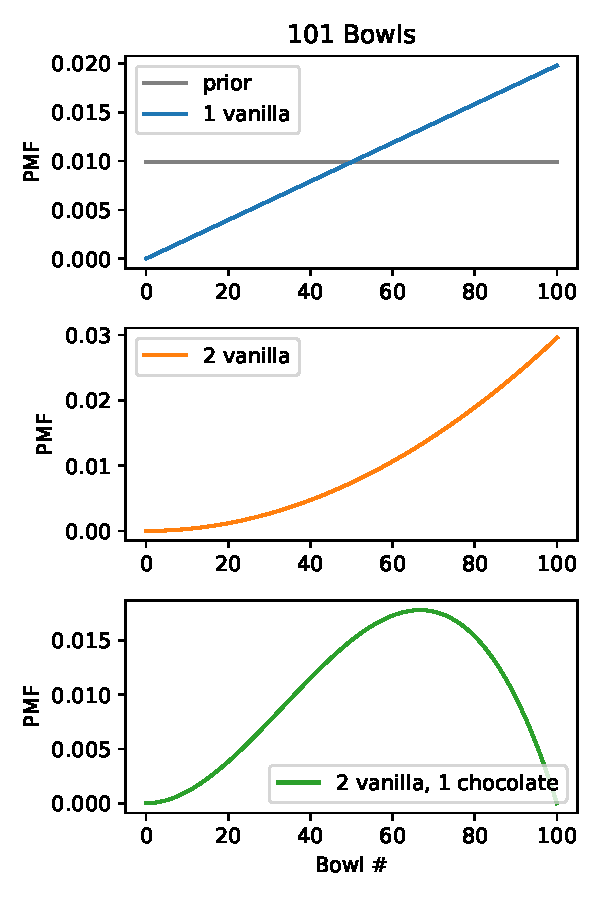
\includegraphics[width=4in]{figs/fig02-01.pdf}}
\caption{Prior and posterior distributions for the 101 Bowls problem.}
\label{fig02-01}
\end{figure}

Suppose we choose a bowl at random, choose a cookie at random, and it turns out to be vanilla.  What is the probability that the cookie came from Bowl \py{x}, for each value of \py{x}?

To solve this problem, I'll use \py{np.arange} to represent 101 hypotheses, numbered from 0 to 100.

\begin{code}
hypos = np.arange(101)
\end{code}

The result is a NumPy array, which we can use to make the prior distribution:

\begin{code}
prior = Pmf(1, hypos)
prior.normalize()
\end{code}

As this example shows, we an initialize a \py{Pmf} with two parameters.
The first parameter is the prior probability; the second parameter is a sequence of values.
Because the probabilities are all the same, we only have to provide one of them.
It gets ``broadcast'' across the hypotheses.

Since all hypotheses have the same prior probability, this distribution is {\bf uniform}.

The likelihood of the data is the fraction of vanilla cookies in each bowl, which we can calculate using \py{hypos}:

\begin{code}
likelihood_vanilla = hypos/100
\end{code}

Now we can compute the posterior distribution in the usual way:

\begin{code}
posterior1 = prior * likelihood_vanilla
posterior1.normalize()
\end{code}

Figure~\ref{fig02-01} (top) shows the prior distribution and the posterior distribution after one vanilla cookie.
Bowl 0 has been eliminated, because it contains no vanilla cookies, and Bowl 100 is the most likely.
The posterior distribution is a line because the the likelihoods are proportional to the bowl numbers.

Now suppose we put the cookie back, draw again from the same bowl, and get another vanilla cookie.
Here's the update after the second cookie:

\begin{code}
posterior2 = posterior1 * likelihood_vanilla
posterior2.normalize()
\end{code}

Figure~\ref{fig02-01} (middle) shows the result.
Because the likelihood function is a line, the posterior after two cookies is a parabola.

At this point the high-numbered bowls are the most likely because they contain the most vanilla cookies, and the low-numbered bowls have been all but eliminated.

But suppose we draw again and get a chocolate cookie.
Here's the update:

\begin{code}
likelihood_chocolate = 1 - hypos/100
posterior3 = posterior2 * likelihood_chocolate
posterior3.normalize()
\end{code}

Figure~\ref{fig02-01} (bottom) shows the result.
Now Bowl 100 has been eliminated because it contains no chocolare cookies.
But the high-numbered bowls are still more likely than the low-numbered bowls, because we have seen more vanilla cookies than chocolate.

In fact, the peak of the posterior distribution is at Bowl 67, which corresponds to the fraction of vanilla cookies in the data we've observed, $2/3$.

The quantity with the highest posterior probability is called the {\bf MAP}, which stands for ``maximum a posteori probability'', where ``a posteori'' is unnecessary Latin for ``posterior''.

To compute the MAP, we can use the \py{Series} method \py{idxmax}:

\begin{code}
posterior3.idxmax()
\end{code}

Or \py{Pmf} provides a more memorable name for the same thing:

\begin{code}
 posterior3.max_prob()
\end{code}

As you might suspect, this example isn't really about bowls; it's about estimating proportions.
Imagine that you have one bowl of cookies.
You don't know what fraction of cookies are vanilla, but you think it is equally likely to be any fraction from 0 to 1.
If you draw three cookies and two are vanilla, what proportion of cookies in the bowl do you think are vanilla?
The posterior distribution we just computed is the answer to that question.

We'll come back to estimating proportions in the next chapter.
But first let's use a \py{Pmf} to solve the dice problem.


\section{The Dice Problem}

In Section~\ref{dice} we solved the dice problem using a Bayes table.
Here's the statment of the problem again:

\begin{quote}
Suppose I have a box with a 6-sided die, an 8-sided die, and a 12-sided die.
I choose one of the dice at random, roll it, and report that the outcome is a 1.
What is the probability that I chose the 6-sided die?
\end{quote}

Let's solve it again using a \py{Pmf}.
I'll use integers to represent the hypotheses:

\begin{code}
hypos = [6, 8, 12]
\end{code}

And I can make the prior distribution like this:

\begin{code}
prior = Pmf(1/3, hypos)
\end{code}

As in the previous example, the prior probability gets broadcast across the hypotheses.

Now we can compute the likelihood of the data:

\begin{code}
likelihood1 = 1/6, 1/8, 1/12
\end{code}

And use it to compute the posterior distribution.

\begin{code}
posterior = prior * likelihood1
posterior.normalize()
\end{code}

Here's the result:

\begin{tabular}{rr}
\toprule
 qs &        ps \\
\midrule
  6 &  0.444444 \\
  8 &  0.333333 \\
 12 &  0.222222 \\
\bottomrule
\end{tabular}


The posterior probability for the 6-sided die is $4/9$.

Now suppose I roll the same die again and get a $7$.
We can do a second update like this:

\begin{code}
likelihood2 = 0, 1/8, 1/12
posterior *= likelihood2
posterior.normalize()
\end{code}

The likelihood for the 6-sided die is $0$ because it is not possible to get a 7 on a 6-sided die.
The other two likelihoods are the same as in the previous update.
And here's the result:

\begin{tabular}{rr}
\toprule
 qs &        ps \\
\midrule
  6 &  0.000000 \\
  8 &  0.692308 \\
 12 &  0.307692 \\
\bottomrule
\end{tabular}


After rolling a 1 and a 7, the posterior probability of the 8-sided die is about 69\%.


\section{Updating Dice}
\label{dice2}

The following function is a more general version of the update in the previous section:

\begin{code}
def update_dice(pmf, data):
    hypos = pmf.qs
    likelihood = 1 / hypos
    impossible = (data > hypos)
    likelihood[impossible] = 0
    pmf *= likelihood
    pmf.normalize()
\end{code}

The first parameter is a \py{Pmf} that represents the possible dice and their probabilities.
The second parameter is the outcome of rolling a die.

The first line selects \py{qs} from the \py{Pmf}, which is the index of the \py{Series}; in this example, it represents the hypotheses.

Since the hypotheses are integers, we can use them to compute the likelihoods.
In general, if there are \py{n} sides on the die, the probability of any possible outcome is \py{1/n}.

However, we have to check for impossible outcomes!
If the outcome exceeds the hypothetical number of sides on the die, the probability of that outcome is $0$.

\py{impossible} is a Boolean Series that is \py{True} for each impossible die.
I use it as an index into \py{likelihood} to set the corresponding probabilities to $0$.

Finally, I multiply \py{pmf} by the likelihoods and normalize.

Here's how we can use this function to compute the updates in the previous section:
 
\begin{code}
pmf = prior.copy()
update_dice(pmf, 1)
update_dice(pmf, 7)
\end{code}

I start with a fresh copy of the prior distribution and use \py{update_dice} to do the updates.
The result is the same.


\section{Summary}

This chapter introduces the \py{empiricaldist} module, which provides \py{Pmf}, which we use to represent a set of hypotheses and their probabilities.

We use a \py{Pmf} to solve the cookie problem and the dice problem, which we saw in the previous chapter.
With a \py{Pmf} it is easy to perform sequential updates as we see multiple pieces of data.

We also solved a more general version of the cookie problem, with 101 bowls rather than two.
Then we computed the MAP, which is the quantity with the highest posterior probability.

In the next chapter ...

But first you might want to work on the exercises.


\section{Exercises}

The code for this chapter is in {\tt chap02.ipynb}, which is in the repository for this book.  See Section~\ref{codeinfo} for details.
You can run the notebook on Colab at \url{https://colab.research.google.com/github/AllenDowney/ThinkBayes2/blob/master/code/chap02.ipynb}.

The notebook provides space where you can work on the following problems.


\begin{exercise}
%TODO: medical test (or maybe chapter 1)
\end{exercise}


\begin{exercise}
Suppose I have a box with a 6-sided die, an 8-sided die, and a 12-sided die.
I choose one of the dice at random, roll it four times, and get 1, 3, 5, and 7.
What is the probability that I chose the 8-sided die?
\end{exercise}


\begin{exercise}
In the previous version of the dice problem, the prior probabilities are the same because the box contains one of each die.
But suppose the box contains 1 die that is 4-sided, 2 dice that are 6-sided, 3 dice that are 8-sided, 4 dice that are 12-sided, and 5 dice that are 20-sided.
I choose a die, roll it, and get a 7.  What is the probability that I chose an 8-sided die?
\end{exercise}


\begin{exercise}
Suppose I have two sock drawers.  
One contains equal numbers of black and white socks.  
The other contains equal numbers of red, green, and blue socks.
Suppose I choose a drawer and random, choose two socks at random, and I tell you that I got a matching pair.
What is the probability that the socks are white?

For simplicity, let's assume that there are so many socks in both drawers that removing one sock makes a negligible change to the proportions.
\end{exercise}


\begin{exercise}
Here's a problem from {\it Bayesian Data Analysis}, which is available from \url{http://www.stat.columbia.edu/~gelman/book}:

\begin{quote}
Elvis Presley had a twin brother (who died at birth). What is the probability that Elvis was an identical twin?
\end{quote}

Hint: In 1935, about 2/3 of twins were fraternal and 1/3 were identical.
\end{exercise}


\chapter{Estimation}
\label{more}

%TODO: Intro


\section{The Euro problem}
\label{euro}

\index{Euro problem}
\index{MacKay, David}
In {\it Information Theory, Inference, and Learning Algorithms}, David MacKay poses this problem:

\begin{quote}
A statistical statement appeared in ``The Guardian'' on Friday January 4, 2002:

  \begin{quote}
        When spun on edge 250 times, a Belgian one-euro coin came
        up heads 140 times and tails 110.  `It looks very suspicious
        to me,' said Barry Blight, a statistics lecturer at the London
        School of Economics.  `If the coin were unbiased, the chance of
        getting a result as extreme as that would be less than 7\%.'
        \end{quote}

But do these data give evidence that the coin is biased rather than fair?
\end{quote}

To answer that question, we'll proceed in two steps.
First we'll use the binomial distribution to see where that 7\% came from; then we'll use Bayes's Theorem to estimate the probability that this coin comes up heads.


\section{The Binomial Distribution}

Suppose we have a coin that we know is fair; if we spin it once, the possible outcomes are heads and tails with equal probability.
I'll denote these outcomes \py{H} and \py{T}.

If you spin it twice, there are four outcomes with equal probability: \py{HH}, \py{HT}, \py{TH}, and \py{TT}. 

If we add up the total number of heads, there are three possible outcomes: 0, 1, or 2.  The probability of 0 and 2 is 25\%, and the probability of 1 is 50\%.

More generally, suppose the probability of heads is \py{p} and we spin the coin \py{n} times.  What is the probability that we get a total of \py{k} heads?

The answer is given by the binomial distribution:
%
\[ P(k; n, p) = \binom{n}{k} p^k (1-p)^{n-k} \]
%
where $\binom{n}{k}$ is the {\bf binomial coefficient}, usually pronounced "n choose k" (see \url{https://en.wikipedia.org/wiki/Binomial_coefficient}).

We can compute this expression ourselves, but we can also use the SciPy function \py{binom.pmf}:

\begin{code}
from scipy.stats import binom

n = 2
p = 0.5
ks = np.arange(n+1)
a = binom.pmf(ks, n, p)
\end{code}

The return value is a NumPy array.
If we put it in a \py{Pmf}, the result is the distribution of \py{k} for the given values of \py{n} and \py{p}.

\begin{code}
pmf_k = Pmf(a, ks)
\end{code}

Here's what it looks like:

\begin{tabular}{rr}
\toprule
 qs &    ps \\
\midrule
  0 &  0.25 \\
  1 &  0.50 \\
  2 &  0.25 \\
\bottomrule
\end{tabular}


We can do the same calculation with \py{n=250}; Figure~\ref{fig03-01} shows the result.

\begin{figure}
% chap03soln.ipynb
\centerline{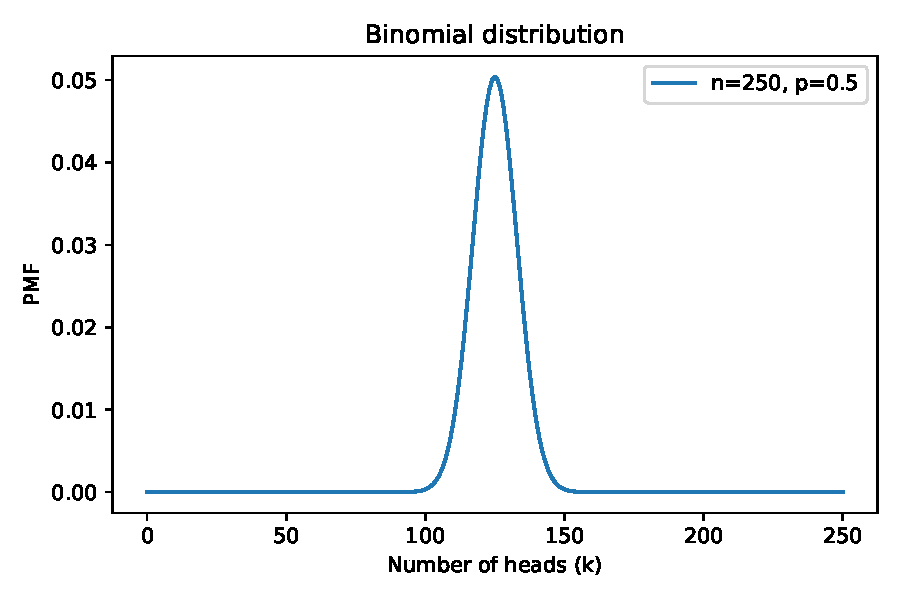
\includegraphics[width=4in]{figs/fig03-01.pdf}}
\caption{Binomial distribution with \py{n=250} and \py{p=0.5}}
\label{fig03-01}
\end{figure}

The most likely outcome is 125, which is \py{n*p}.
But the probability of getting exactly 125 heads is only about 5\%.
The probability of getting 140 heads, as in the Euro problem is lower, around 0.8\%, but it is still possible even if the coin is fair.

In the article MacKay quotes, the statistician says, ``If the coin were unbiased the chance of getting a result as extreme as that would be less than 7\%''.

We can use the binomial distribution to check his math.  The following function takes a PMF and computes the total probability of values greater than or equal to \py{threshold}. 

\begin{code}
def ge_dist(pmf, threshold):
    ge = (pmf.index >= threshold)
    total = pmf[ge].sum()
    return total
\end{code}

We can call it like this:

\begin{code}
ge_dist(pmf_k, 140)
\end{code}

Or \py{Pmf} provides a function that computes the same thing:

\begin{code}
pmf_k.ge_dist(140)
\end{code}

Either way, the probability is about 3.3\% that we get 140 heads or more.
But that's less than 7%.  

The reason is that the statistician includes all values ``as extreme as'' 140, which includes values less than or equal to 110, because 140 exceeds the expected value by 15 and 110 falls short by 15.

The probability of values less than or equal to 110 is also 3.3\%,
so the total probability of values ``as extreme'' as 140 is 6.6\%.

The point of this calculation is that these extreme values are unlikely if the coin is fair.
And that's why the statistician concludes that the results are ``very suspicious''.

That's interesting, but it doesn't answer MacKay's question.  So let's move on to the next step, estimating the proportion of heads.


\section{Estimating Proportions}
\label{estprop}

Any given coin has some probability of landing heads up when spun
on edge; I'll call this probability \py{x}.

It seems reasonable to believe that \py{x} depends
on physical characteristics of the coin, like the distribution
of weight.

If a coin is perfectly balanced, we expect \py{x} to be close to 50\%, but
for a lopsided coin, \py{x} might be substantially different.  We can use
Bayes's theorem and the observed data to estimate \py{x}.

For simplicity, I'll start with a uniform prior, which assume that all values of \py{x} are equally likely.
That might not be a reasonable assumption, so we'll come back and consider other priors later.

Here's the uniform prior:

\begin{code}
hypos = np.arange(0, 101)
prior = Pmf(1, hypos)
\end{code}

And here are the likelihoods:

\begin{code}
likelihood = {
    'H': hypos/100,
    'T': 1 - hypos/100
}
\end{code}

I put the likelihoods for heads and tails in a dictionary to make it easier to do the update.

To represent the data, I'll use a list of strings, where each string is \py{H} or \py{T}:

\begin{code}
dataset = 'H' * 140 + 'T' * 110
\end{code}

The following function does the update.

\begin{code}
def update_euro(pmf, dataset):
    for data in dataset:
        pmf *= likelihood[data]

    pmf.normalize()
\end{code}

The first argument is a \py{Pmf} that represents the prior.
The second argument is a list of strings.
Each time through the loop, we multiply \py{pmf} by the likelihood of one outcome, heads or tails.

Notice that \py{normalize} is outside the loop, so the posterior distribution only gets normalized one, at the end.
That's more efficient than normalizing it after each spin (although we'll see later that it can also cause problems with floating-point arithmetic).
%TODO:  add forward reference

Here's how we do the update:

\begin{code}
posterior = prior.copy()
update_euro(posterior, dataset)
\end{code}

Figure~\ref{fig03-02} shows the posterior distribution of \py{x}.

\begin{figure}
% chap03soln.ipynb
\centerline{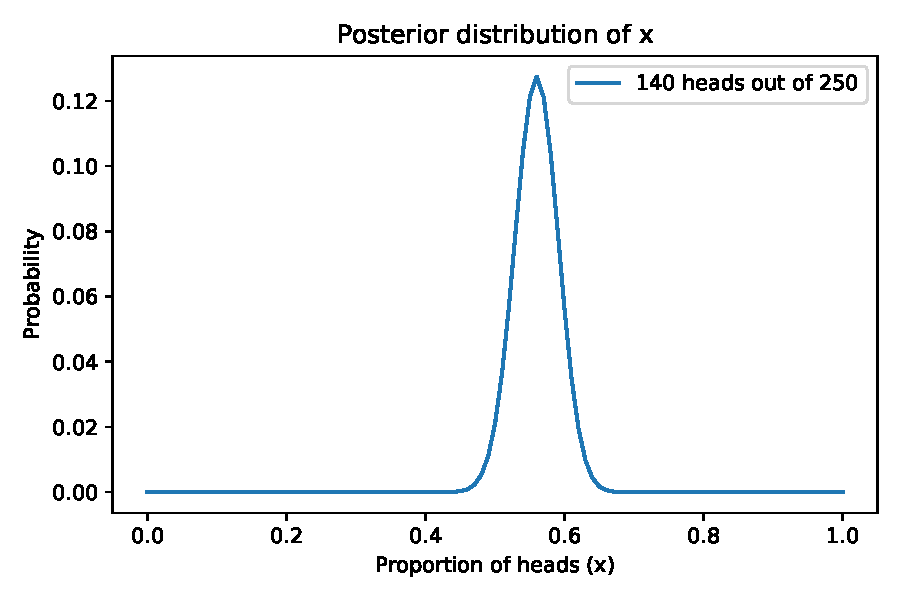
\includegraphics[width=4in]{figs/fig03-02.pdf}}
\caption{Posterior distribution of \py{x} after 140 heads in 250 spins.}
\label{fig03-02}
\end{figure}

Now, it's easy to get this distribution mixed up with the previous one, but rememeber:

\begin{itemize}

\item Figure~\ref{fig03-01} shows the distribution of \py{k}, which is the number of heads we get with \py{n=250} and \py{p=0.5}.

\item Figure ~\ref{fig03-02} shows the posterior distribution of \py{x} which is the proportion of heads for the coin we observed. 

\end{itemize}

The posterior distribution represents our beliefs about \py{x} after seeing the data.
It indicates that values less than 40 and greater than 80 are unlikely; values between 50 and 60 are the most likely.

In fact, the most likely value for \py{x} is 56\% which is the proportion of heads in the dataset, \py{140/250}.


\section{Triangle Prior}
\label{triangle}

So far we've been using a uniform prior, but that might not be a reasonable choice based on what we know about coins.  
I can believe that if a coin is lopsided, \py{x} might deviate substantially from 50\%, but it seems unlikely that the Belgian Euro coin is so imbalanced that \py{x} is 10\% or 90\%.

It might be more reasonable to choose a prior that gives
higher probability to values of \py{x} near 50\% and lower probability
to extreme values.

\index{triangle distribution}

As an example, let's try a triangule-shaped prior.
Here's the code that constructs it:

\begin{code}
ramp_up = np.arange(50)
ramp_down = np.arange(50, -1, -1)
a = np.append(ramp_up, ramp_down)

triangle = Pmf(a, hypos, name='triangle')
triangle.normalize()
\end{code}

\py{arange} returns a NumPy array, so we can use \py{np.append} to append \py{ramp_down} to the end of \py{ramp_up}.
Then we use \py{a} and \py{hypos} to make a \py{Pmf}.

Figure~\ref{fig03-03} shows the result, along with the uniform distribution.
 
\begin{figure}
% chap03soln.ipynb
\centerline{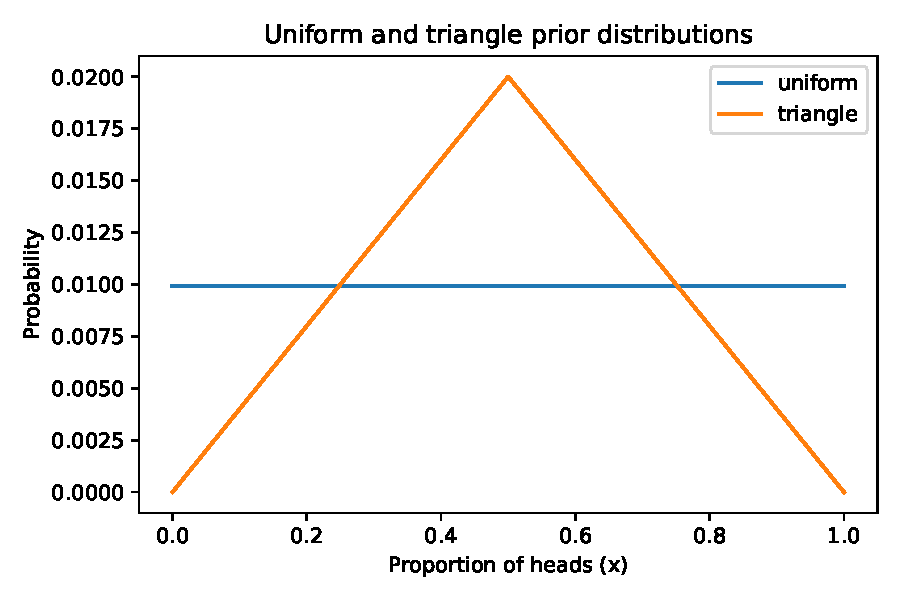
\includegraphics[width=4in]{figs/fig03-03.pdf}}
\caption{Uniform and trianlge-shaped prior distributions.}
\label{fig03-03}
\end{figure}

Now we can update both priors with the same data: 
 
\begin{code}
update_euro(uniform, dataset)
update_euro(triangle, dataset)
\end{code}

Figure~\ref{fig03-04} shows the posterior distributions.

\begin{figure}
% chap03soln.ipynb
\centerline{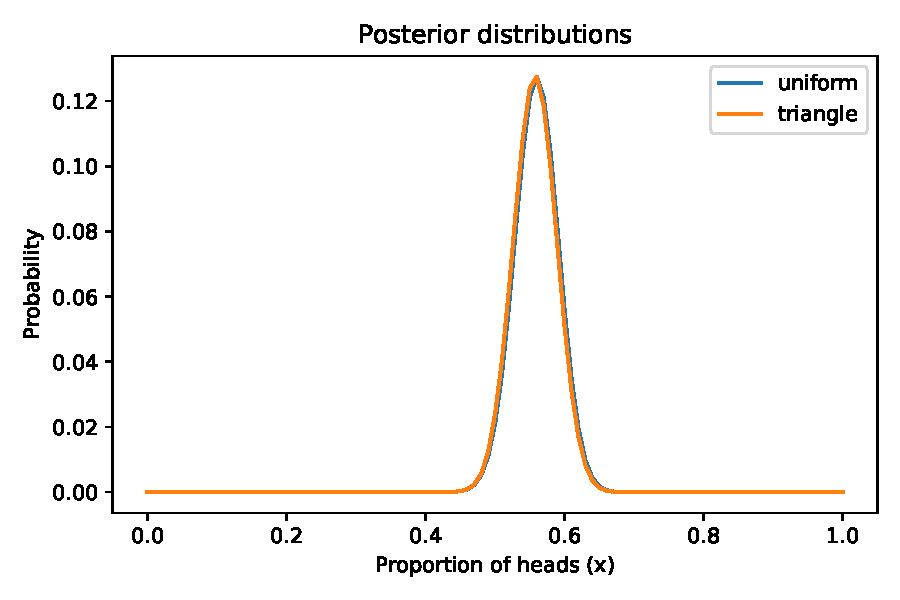
\includegraphics[width=4in]{figs/fig03-04.pdf}}
\caption{Posterior distributions based on uniform and triangle priors.}
\label{fig03-04}
\end{figure}

The differences between the posterior distributions are barely visible, and so small they would hardly matter in practice.

And that's good news.
To see why, imagine two people who disagree angrily about which prior is better, uniform or triangle.
Each of them has reasons for their preference, but neither of them can persuade the other to change their mind.

But suppose they agree to use the data to update their beliefs.
When they compare their posterior distributions, they find that there is almost nothing left to argue about.

This is an example of {\bf swamping the priors}: with enough
data, people who start with different priors will tend to
converge on the same posterior distribution.

\index{swamping the priors}
\index{convergence}


\section{Binomial Likelihood}

So far we've been computing the updates one spin at a time, so we have to 

A more efficient alternative is to compute the likelihood of the entire dataset at once.
For each hypothetical value of \py{x}, we have to compute the probability of getting 140 heads out of 250 spins.

Well, we know how to do that.  This is the question the binomial distribution answer.
If the probability of heads is $p$, the probability of $k$ heads in $n$ spins is:
%
\[ P(k; n, p) = \binom{n}{k} p^k (1-p)^{n-k} \]
%
And we can use SciPy to compute it.
The following function takes a \py{Pmf} that represents a prior distribution and a tuple of integers, \py{k} and \py{n}:

\begin{code}
from scipy.stats import binom

def update_binomial(pmf, data):
    k, n = data
    xs = pmf.qs
    likelihood = binom.pmf(k, n, xs)
    pmf *= likelihood
    pmf.normalize()
\end{code}

It extracts the hypothetical values of \py{x} from the \py{Pmf} and passes them to `binom.pmf`, which computes the binomial PMF for the given values of \py{k} and \py{n}, and all values of \py{x}.

Here's how we use it:

\begin{code}
uniform2 = Pmf(1, hypos)
data = 140, 250
update_binomial(uniform2, data)
\end{code}

The result is the same as in Section~\ref{estprop} except for a small floating-point round-off.


\section{Bayesian Statistics}

You might have noticed some similarity between the Euro problem and the 101 bowls problem in Section~\ref{morebowls}.
The prior distributions are the same, the likelihoods are the same, and with the same data the results would be the same.

But there are two differences.

The first is the choice of the prior.
In the 101 bowls problem, the uniform prior is implied by the statement of the problem, which says that we choose one of the bowls at random with equal probability.

In the Euro problem, the choice of the prior is subjective; that is, reasonable people could disagree, maybe because they have different information about coins or because they interpret the same information differently.

Because the priors are subjective, the posteriors are subjective, too.
And some people find that problematic.

The other difference is the nature of what we are estimating.
In the 101 bowls problem, we choose the bowl randomly, so it is uncontroversial to compute the probability of choosing each bowl.
In the Euro problem, the proportion of heads is a physical property of a given coin.
Under some interpretations of probability, that's a problem because physical properties are not considered random.

As an example, consider the age of the universe.
Currently, our best estimate is 13.80 billion years, but it might be off by 0.02 billion years in either direction (see \url{https://en.wikipedia.org/wiki/Age_of_the_universe}).

Now suppose we would like to know the probability that the age of the universe is actually greater than 13.81 billion years.
Under some interpretations of probability, we would not be able to answer that question.
We would be required to say something like, ``The age of the universe is not a random quantity, so it has no probability of exceeding any particular value.''

Under the Bayesian interpretation of probability, it is meaningful and useful to treat physical quantities as if they were random and compute probabilities about them.

In the Euro problem, the prior distribution represents what we believe about coins in general and the posterior distribution represents what we believe about a particular coin after seeing the data.
So we can use the posterior distribution to compute probabilities about the coin and its proportion of heads.

These differences, the subjectivity of the prior and the interpretation of the posterior, are key differences between Bayes's Theorem and Bayesian statistics.

Bayes's Theorem is a mathematical law of probability; no reasonable person objects to it.
But Bayesian statistics is surprisingly controversial.
Historically, many people have been bothered by its subjectivity and its use of probability for things that are not random.

If you are interested in this history, I recommend Sharon Bertsch McGrayne's book, {\it The Theory That Would Not Die} (\url{https://yalebooks.yale.edu/book/9780300188226/theory-would-not-die}).

\index{McGrayne, Sharon Bertsch}
\index{The Theory That Would Not Die}

%TODO: Italicize the index entry

\section{Summary}

In this chapter I posed David MacKay's Euro problem and we started to solve it.
Given the data, we computed the posterior distribution for \py{x}, the probability a Euro coin comes up heads.

We computed the posterior distribution with two different priors and found that the posteriors were nearly the same.
This is good news, because it suggests that if two people start with different beliefs but they see the same data, their beliefs will tend to converge.

This chapter introduces the binomial distribution, which we used to compute the posterior distribution more efficiently.
And I discussed the difference between applying Bayes's Theorem, as in the 101 bowls problem, and computing Bayesian statistics, as in the Euro problem.

\index{convergence}

However, we still haven't answered MacKay's question: ``Do these data give evidence that the coin is biased rather than fair?''
I'm going to leave this question hanging a little longer; we'll come back to it in Chapter~\ref{hypotest}.

In the next chapter, I want to get back to the dice problem.

\section{Exercises}

The code for this chapter is in {\tt chap03.ipynb}, which is in the repository for this book.  See Section~\ref{codeinfo} for details.
You can run the notebook on Colab at \url{https://colab.research.google.com/github/AllenDowney/ThinkBayes2/blob/master/code/chap03.ipynb}.

The notebook provides space where you can work on the following problems.


\begin{exercise}
In major league baseball, most players have a batting average between 200 and 330, which means that the probability of getting a hit is between 0.2 and 0.33.

Suppose a new player appearing in his first game gets 3 hits out of 3 attempts.  What is the posterior distribution for his probability of getting a hit?
\end{exercise}


\begin{exercise}
Whenever you survey people about sensitive issues, you have to deal with ``social desirability bias'', which is the tendency of people to shade their answers to show themselves in the most positive light (see \url{https://en.wikipedia.org/wiki/Social_desirability_bias}).

One of the ways to improve the accuracy of the results is ``randomized response'' (see \url{https://en.wikipedia.org/wiki/Randomized_response}).

As an example, suppose you ask 100 people to flip a coin and:

\begin{itemize}

\item If they get heads, they report YES.

\item If they get tails, they honestly answer the question ``Do you cheat on your taxes?''

\end{itemize}

And suppose you get 80 YESes and 20 NOs.  Based on this data, what is the posterior distribution for the fraction of people who cheat on their taxes?  What is the most likely value in the posterior distribution?
\end{exercise}


\begin{exercise}
Suppose that instead of observing coin spins directly, you measure the outcome using an instrument that is not always correct.  Specifically, suppose the probability is \py{y=0.2} that an actual heads is reported
as tails, or actual tails reported as heads.

If we spin a coin 250 times and the instrument reports 140 heads, what is the posterior distribution of \py{x}?

What happens as you vary the value of \py{y}?
\end{exercise}


\begin{exercise}
In preparation for an alien invasion, the Earth Defense League (EDL) has been working on new missiles to shoot down space invaders.  Of course, some missile designs are better than others; let's assume that each design has some probability of hitting an alien ship, \py{x}.

Based on previous tests, the distribution of \py{x} in the population of designs is approximately uniform between 0.1 and 0.4.

Now suppose the new ultra-secret Alien Blaster 9000 is being tested.  In a press conference, an EDL general reports that the new design has been tested twice, taking two shots during each test.  The results of the test are confidential, so the general won't say how many targets were hit, but they report: ``The same number of targets were hit in the two tests, so we have reason to think this new design is consistent.''

Is this data good or bad; that is, does it increase or decrease your estimate of \py{x} for the Alien Blaster 9000?

Hint: If the probability of hitting each target is $x$, the probability of hitting one target in both tests is $[2x(1-x)]^2$.
\end{exercise}


\chapter{More Estimation}
\label{estimation}

\section{The train problem}

\index{train problem}
\index{Mosteller, Frederick}
\index{German tank problem}

I found the train problem 
in Frederick Mosteller's, {\it Fifty Challenging Problems in
  Probability with Solutions} (\url{https://store.doverpublications.com/0486653552.html}):

\begin{quote}
``A railroad numbers its locomotives in order $1..N$.  One day you see a
locomotive with the number 60.  Estimate how many locomotives the
railroad has.''
\end{quote}

Based on this observation, we know the railroad has 60 or more
locomotives.  But how many more?  To apply Bayesian reasoning, we
can break this problem into two steps:

\begin{enumerate}

\item What did we know about $N$ before we saw the data?

\item For any given value of $N$, what is the likelihood of
seeing the data (a locomotive with number 60)?

\end{enumerate}

The answer to the first question is the prior.  The answer to the
second is the likelihood.

\begin{figure}
% train.py
\centerline{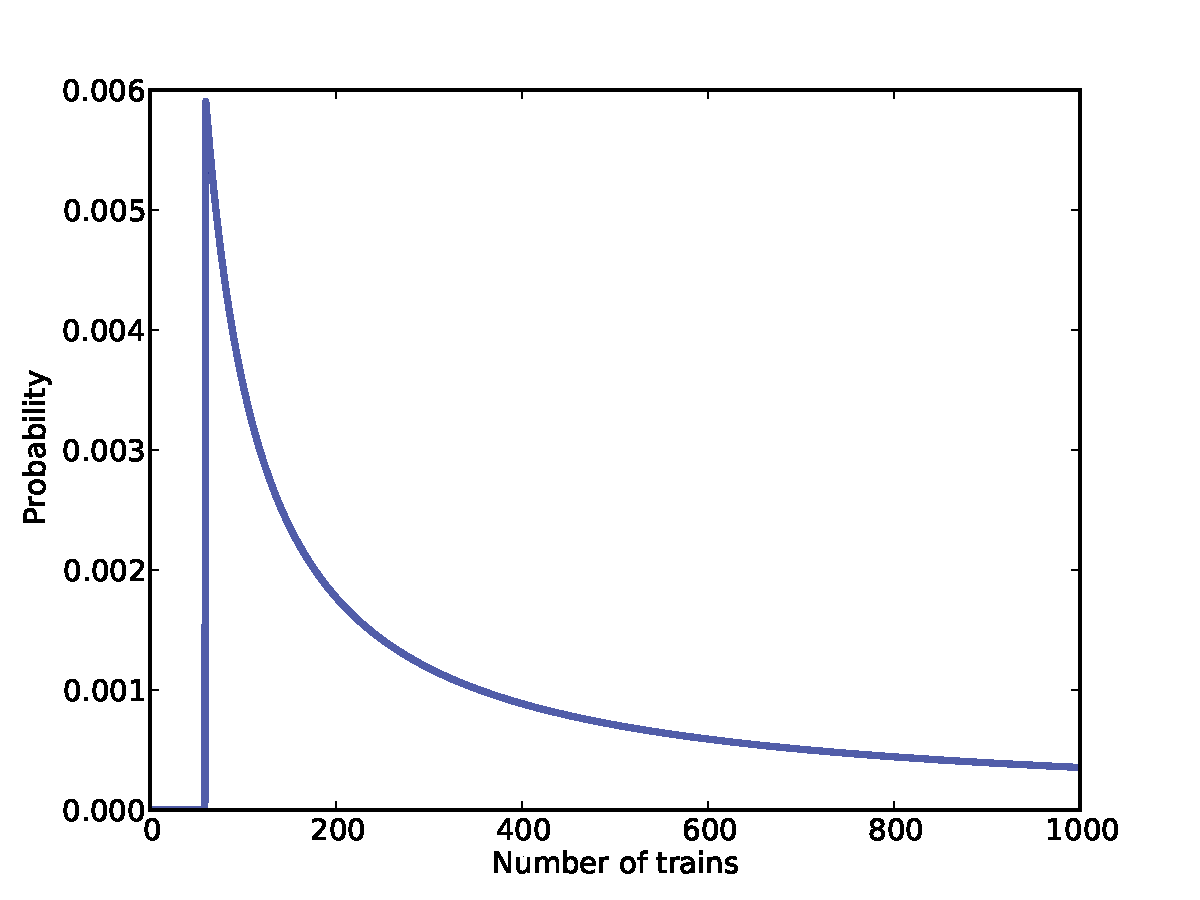
\includegraphics[height=2.5in]{figs/train1.pdf}}
\caption{Posterior distribution for the locomotive problem, based
on a uniform prior.}
\label{fig.train1}
\end{figure}

We don't have much basis to choose a prior, so let's start with
something simple and then consider alternatives.  Let's assume that
$N$ is equally likely to be any value from 1 to 1000.

\begin{code}
hypos = np.arange(1, 1001)
prior = Pmf(1, hypos)
\end{code}

Now let's figure out the likelihood of the data.
In a hypothetical fleet of $N$ locomotives, what is the probability that we would see number 60?
If we assume that we are equally likely to see any
locomotive, the chance of seeing any particular one is
$1/N$.

Here's the function that does the update:

\begin{code}
def update_train(pmf, data):
    hypos = pmf.qs
    likelihood = 1 / hypos
    impossible = (data > hypos)
    likelihood[impossible] = 0
    pmf *= likelihood
    pmf.normalize()
\end{code}

The first parameter is a \py{Pmf} that represents the possible values of $N$ and their probabilities.
The second parameter is the number of the train we observed.

This function might look familiar; it is the same as the update function for the dice problem in Section~\ref{dice2}.

\index{dice problem}

Here's the update:

\begin{code}
data = 60
posterior = prior.copy()
update_train(posterior, data)
\end{code}

Figure~\ref{fig04-01} shows the results.
 
\begin{figure}
% chap04soln.ipynb
\centerline{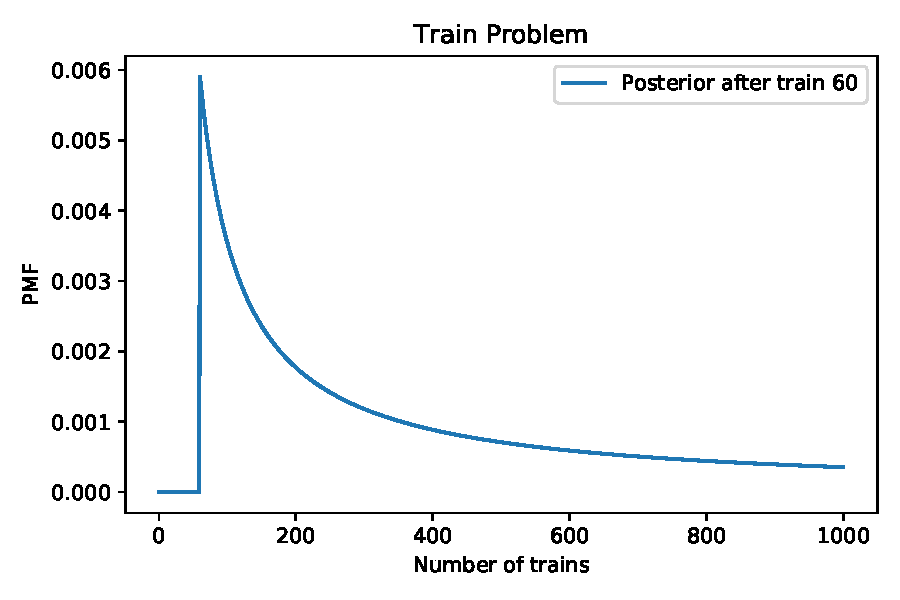
\includegraphics[width=4in]{figs/fig04-01.pdf}}
\caption{Posterior distribution of the number of trains, $N$, after seeing train number 60.}
\label{fig04-01}
\end{figure}

Not surprisingly, all
values of $N$ below 60 have been eliminated.

The most likely value, if you had to guess, is 60.  
That might not seem like a very good guess; after all, what are the chances that you just happened to see the train with the highest number?
Nevertheless, if you want to maximize the chance of getting
the answer exactly right, you should guess 60.

But maybe that's not the right goal.  
An alternative is to compute the mean of the posterior distribution.
Given a set of possible quantities, $q_i$, and their probabilities, $p_i$, the mean of the distribution is:
%
\[ \mathrm{mean} = \sum_i p_i q_i \]
%
Which we can compute like this:

\begin{code}
np.sum(posterior.ps * posterior.qs)
\end{code}

Or {\tt Pmf} provides a function that does the same thing:

\begin{code}
posterior.mean()
\end{code}

The mean of the posterior is 333, so that might be a good guess if you want to minimize error.  
If you played this guessing game over and over, using the mean of the posterior as your estimate would minimize the mean squared error over the long run (see \url{http://en.wikipedia.org/wiki/Minimum_mean_square_error}).

\index{mean squared error}


\section{What about that prior?}

The prior I chose in the previous section is uniform from 1 to 1000, but I offered no justification for choosing 1000, or for choosing a uniform
distribution.

\index{prior distribution}

It is reasonable to believe that a railroad company might operate 1000 locomotives, but it might be just as reasonable to think they have 500, or 2000.
So we might wonder whether the posterior distribution is sensitive to the prior.  
With so little data---only one observation---it probably is.

\begin{itemize}

\item With a uniform prior from 1 to 1000, the posterior mean is 207.

\item With an upper bound of 1000, it's 333.

\item With an upper bound of 2000, it's 552.

\end{itemize}

So that's bad.  
When the posterior is sensitive to the prior, there are two ways to proceed:

\begin{itemize}

\item Get more data.

\item Get more background information.

\end{itemize}

With more data, posterior distributions based on different
priors tend to converge.  
For example, suppose that in addition
to train 60 we also see trains 30 and 90.  
We can update the distribution like this:

\begin{code}
for data in [30, 60, 90]:
    update_train(pmf, data)
\end{code}

With these data, the means of the posteriors are

\begin{tabular}{r r}
\toprule
Upper & Posterior \\
Bound & Mean \\
\midrule
500 & 152 \\
1000 & 164\\
2000 & 171\\
\bottomrule
\end{tabular}

The differences are smaller, but apparently three trains is not enough for the posteriors to converge.


\section{Another prior}

\begin{figure}
% train.py
\centerline{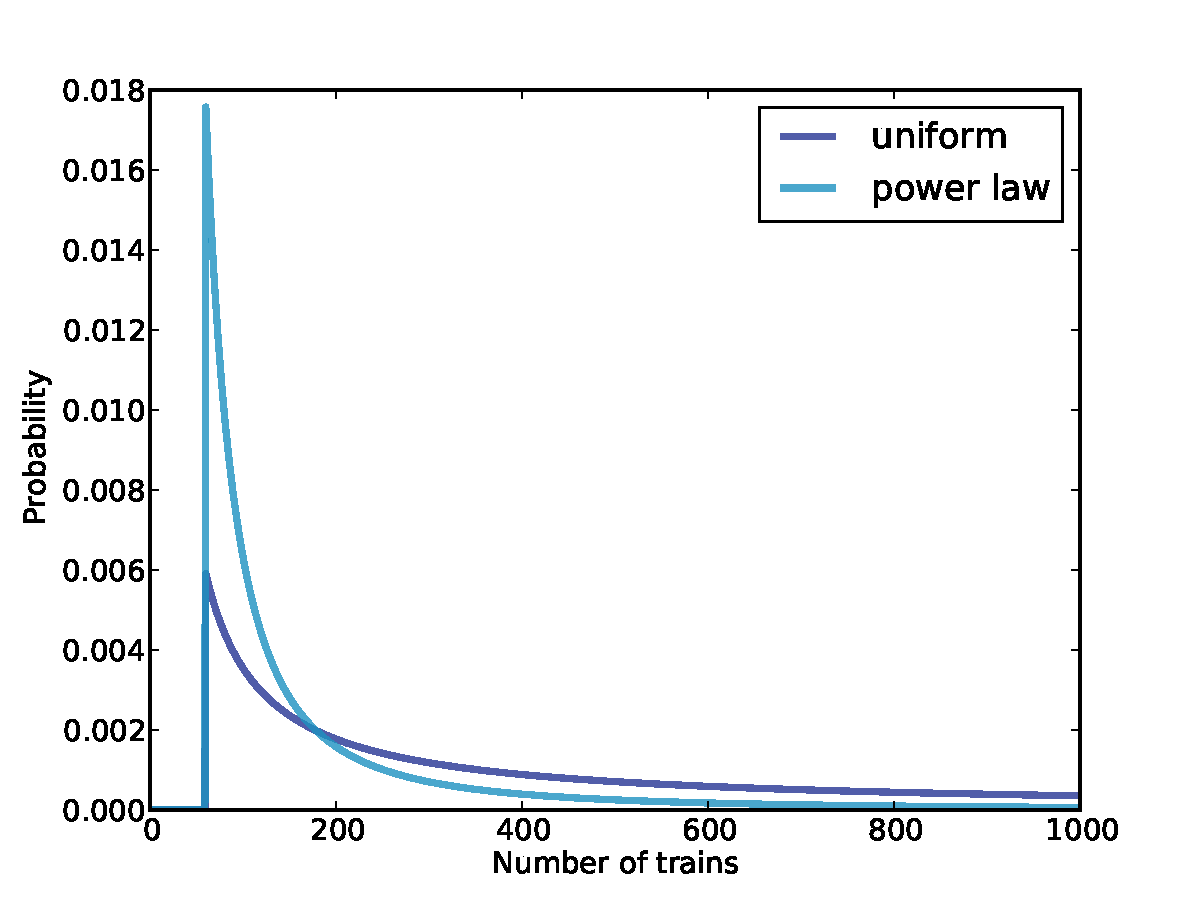
\includegraphics[height=2.5in]{figs/train4.pdf}}
\caption{Posterior distribution based on a power law prior,
compared to a uniform prior.}
\label{fig.train4}
\end{figure}

If more data are not available, another option is to improve the
priors by gathering more background information.  
It is probably not reasonable to assume that a train-operating company with 1000 locomotives is just as likely as a company with only 1.

With some effort, we could probably find a list of companies that
operate locomotives in the area of observation.
Or we could interview an expert in rail shipping to gather information about the typical size of companies.

But even without getting into the specifics of railroad economics, we
can make some educated guesses.  
In most fields, there are many small
companies, fewer medium-sized companies, and only one or two very
large companies.  
In fact, the distribution of company sizes tends to
follow a power law, as Robert Axtell reports in {\it Science} (see
\url{https://sci-hub.tw/10.1126/science.1062081}).

% \url{http://www.sciencemag.org/content/293/5536/1818.full.pdf}

\index{power law}
\index{Axtell, Robert}

This law suggests that if there are 1000 companies with fewer than
10 locomotives, there might be 100 companies with 100 locomotives,
10 companies with 1000, and possibly one company with 10,000 locomotives.

Mathematically, a power law means that the number of companies
with a given size is inversely proportional to size, or
%
\[ \PMF(N) \propto \left( \frac{1}{N} \right)^{\alpha}   \]
%
where $\PMF(N)$ is the probability mass function of $N$ and $\alpha$ is
a parameter that is often near 1.

We can construct a power law prior like this:

\begin{code}
alpha = 1.0
hypos = np.arange(1, 1001)
ps = hypos**(-alpha)
power = Pmf(ps, hypos, name='power law')
power.normalize()
\end{code}

Again, the upper bound is arbitrary, but with a power law prior, the posterior is less sensitive to this choice.

\begin{figure}
% chap04soln.ipynb
\centerline{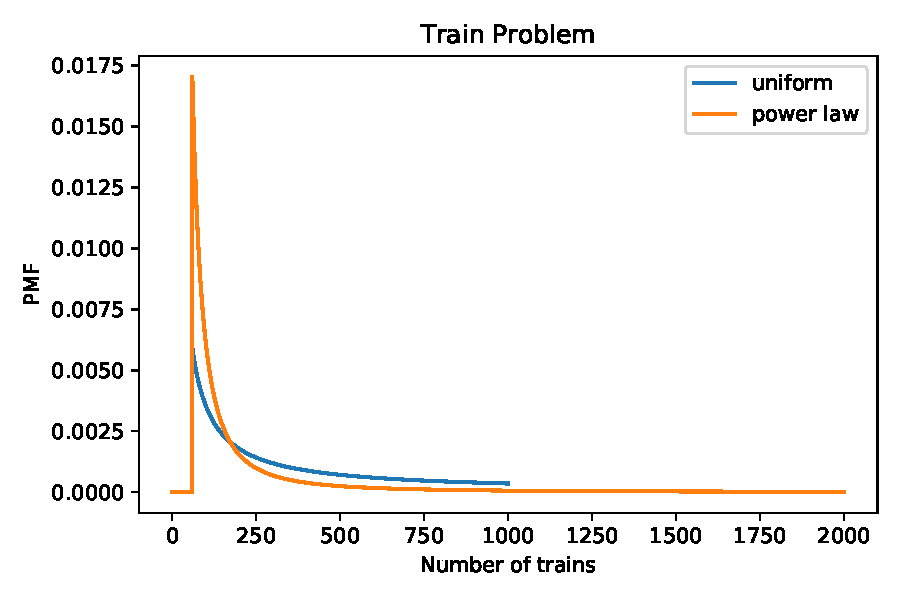
\includegraphics[width=4in]{figs/fig04-02.pdf}}
\caption{Posterior distributions for the uniform and power law priors
after seeing train 60.}
\label{fig04-02}
\end{figure}

Figure~\ref{fig04-02} shows the new posterior based on the power law prior, compared to the posterior based on the uniform prior, both after seeing train number 60.

With the power law prior, we assign higher probability to smaller numbers of trains.
And the posterior is less sensitive to the choice of the upper bound.
If we observe trains 30, 60, and 90, the means of the posteriors are

\begin{tabular}{rr}
\toprule
Upper & Posterior \\
Bound & Mean \\
\midrule
  500 & 131 \\
  1000 & 133 \\
  2000 & 134 \\
\bottomrule
\end{tabular}

Now the differences are much smaller.  In fact,
with an arbitrarily large upper bound, the mean converges on 134.

So the power law prior is more realistic, because it is based on
general information about the size of companies, and it
behaves better in practice.


\section{Credible intervals}
\label{credible}

Once you have computed a posterior distribution, it is often useful
to summarize the results with a single point estimate or an interval.
For point estimates it is common to use the mean, median, or the
value with maximum posterior probability.

\index{credible interval}
\index{maximum likelihood}

For intervals we often choose two values so that there is a 90\% chance that the estimated value falls between them (or some other probability).
These values define a {\bf credible interval} or {\bf CI}.

\py{Pmf} provides a function called \py{credible_interval} that takes a probability and computes an interval that contains that probability.
To compute a 90\% CI, we can call it like this:

\index{percentile}

\begin{code}
posterior.credible_interval(0.9)
\end{code}

For the previous example---the locomotive problem with a power law prior
and three trains---the 90\% credible interval is $(91, 242)$.  The
width of this range suggests, correctly, that we are still quite
uncertain about how many locomotives there are.

\py{credible_interval} uses another function called \py{quantile} that takes a probability and returns a value.
If the probability is 0.05, it returns the 5th percentile; for example,
\py{power.quantile(0.05)} returns 91, which means that there's a 5\% chance that the number of trains is less than or equal to 91.

And \py{power.quantile(0.95)} returns 242, so there's a 95\% chance that the number of trains is less than or equal to 242.

Putting those results together, there's a 90\% chance that the number of trains falls between 91 and 242.

The next section explains how \py{quantile} works.


\section{Cumulative distribution functions}

%TODO: Do a better job explaining the CDF

\py{quantile} is based on the {\bf cumulative distribution function}, or CDF, which is the cumulative sum of the PMF.
If we compute $CDF(x)$ the result is the probability that the estimated value is less than or equal to $x$.

\index{cumulative distribution function}
\index{CDF}

\py{Pmf} provides \py{make_cdf}, which returns a \py{Cdf} object.
I'll use CDF and PMF for the mathematical concepts and \py{Pmf} and \py{Cdf} for the classes defined in \py{empiricaldist}.

Figure~\ref{fig04-03} shows the CDF of the posterior distribution from the previous section.

\begin{figure}
% chap04soln.ipynb
\centerline{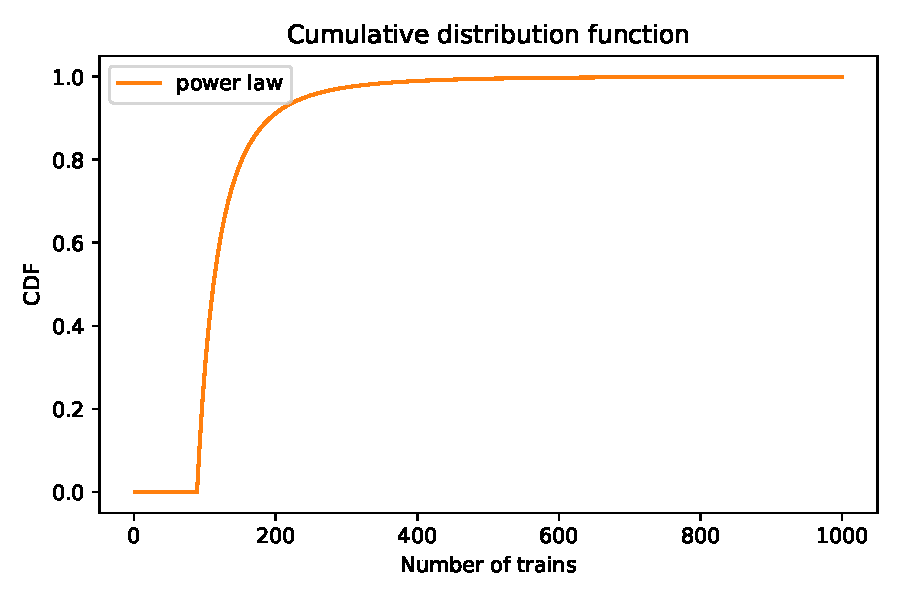
\includegraphics[width=4in]{figs/fig04-03.pdf}}
\caption{Cumulative distribution function (CDF) for the posterior distribution based on the power law prior.}
\label{fig04-03}
\end{figure}

The $y$-axis shows cumulative probabilities from 0 to 1.

CDFs and PMFs are equivalent in the sense that they contain the
same information about the distribution, and you can always convert
from one to the other.  
The advantage of the CDF is that it computes percentiles more efficiently.

\section{The German tank problem}

During World War II, the Economic Warfare Division of the American
Embassy in London used statistical analysis to estimate German
production of tanks and other equipment.\footnote{Ruggles and Brodie,
  ``An Empirical Approach to Economic Intelligence in World War II,''
  {\em Journal of the American Statistical Association}, Vol. 42,
  No. 237 (March 1947).}

The Western Allies had captured log books, inventories, and repair
records that included chassis and engine serial numbers for individual
tanks.

Analysis of these records indicated that serial numbers were allocated
by manufacturer and tank type in blocks of 100 numbers, that numbers
in each block were used sequentially, and that not all numbers in each
block were used.  So the problem of estimating German tank production
could be reduced, within each block of 100 numbers, to a form of the
locomotive problem.

Based on this insight, American and British analysts produced
estimates substantially lower than estimates from other forms
of intelligence.  And after the war, records indicated that they were
substantially more accurate.

They performed similar analyses for tires, trucks, rockets, and other
equipment, yielding accurate and actionable economic intelligence.

The German tank problem is historically interesting; it is also a nice
example of real-world application of statistical estimation.  So far
many of the examples in this book have been toy problems, but it will
not be long before we start solving real problems.  I think it is an
advantage of Bayesian analysis, especially with the computational
approach we are taking, that it provides such a short path from a
basic introduction to the research frontier.


\section{Discussion}

Among Bayesians, there are two approaches to choosing prior
distributions.  Some recommend choosing the prior that best represents
background information about the problem; in that case the prior
is said to be {\bf informative}.  The problem with using an informative
prior is that people might use different background information (or
interpret it differently).  So informative priors often seem subjective.
\index{informative prior}

The alternative is a so-called {\bf uninformative prior}, which is
intended to be as unrestricted as possible, in order to let the data
speak for themselves.  In some cases you can identify a unique prior
that has some desirable property, like representing minimal prior
information about the estimated quantity.
\index{uninformative prior}

Uninformative priors are appealing because they seem more
objective.  But I am generally in favor of using informative priors.
Why?  First, Bayesian analysis is always based on
modeling decisions.  Choosing the prior is one of those decisions, but
it is not the only one, and it might not even be the most subjective.
So even if an uninformative prior is more objective, the entire analysis
is still subjective.

\index{modeling}
\index{subjectivity}
\index{objectivity}

Also, for most practical problems, you are likely to be in one of two
regimes: either you have a lot of data or not very much.  If you have
a lot of data, the choice of the prior doesn't matter very much;
informative and uninformative priors yield almost the same results.
We'll see an example like this in the next chapter.

But if, as in the locomotive problem, you don't have much data,
using relevant background information (like the power law distribution)
makes a big difference.
\index{locomotive problem}

And if, as in the German tank problem, you have to make life-and-death
decisions based on your results, you should probably use all of the
information at your disposal, rather than maintaining the illusion of
objectivity by pretending to know less than you do.
\index{German tank problem}


\section{Exercises}

\begin{exercise}
Something with CDFs and credible intervals
\end{exercise}

\begin{exercise}
I often see rabbits in the garden behind my house, but it's not easy to tell them apart, so I don't really know how many rabbits there are.

Suppose I deploy a motion-sensing camera trap that takes a picture of the first rabbit it sees each day.  After three days, I compare the pictures and conclude that two of them are the same rabbit and the other is different.

How many rabbits visit my garden?

To answer this question, we have to think about the prior distribution and the likelihood of the data:

\begin{itemize}

\item I have sometimes seen four rabbits at the same time, so I know there are at least that many.  I would be surprised if there were more than 10.  So, at least as a starting place, I think a uniform prior from 4 to 10 is reasonable.

\item To keep things simple, let's assume that all rabbits who visit my garden are equally likely to be caught by the camera trap in a given day.  Let's also assume it is guaranteed that the camera trap gets a picture every day.

\end{itemize}

\end{exercise}

\begin{exercise}
Suppose that in the criminal justice system, all prison sentences are either 1, 2, or 3 years, with an equal number of each.  One day, you visit a prison and choose a prisoner at random.  What is the probability that they are serving a 3-year sentence?  What is the average remaining sentence of the prisoners you observe?
\end{exercise}


\begin{exercise}
If I chose a random adult in the U.S., what is the probability that they have a sibling? To be precise, what is the probability that their mother has had at least one other child.

This article from the Pew Research Center provides some relevant data: \url{https://www.pewsocialtrends.org/2015/05/07/family-size-among-mothers}.  You will have to make some simplifying assumptions.
\end{exercise}


\begin{exercise}
The Doomsday argument is ``a probabilistic argument that claims to predict the number of future members of the human species given an estimate of the total number of humans born so far.''  See \url{https://en.wikipedia.org/wiki/Doomsday_argument}.

Suppose there are only two kinds of civilizations that can happen in the universe. The ``short-lived'' kind go exinct after only 200 billion individuals are born. The ``long-lived'' kind survive until 2,000 billion individuals are born. And suppose that the two kinds of civilization are equally likely.  Which kind of civilization do you think we live in? 

The Doomsday argument says we can use the total number of humans born so far as evidence.
According to the Population Reference Bureau, the total number of people who have ever lived is about 108 billion. 

Since you were born quite recently, let's assume that you are, in fact, human being number 108 billion.
If $N$ is the total number who will ever live and we consider you to be a randomly-chosen person, it is equally likely that you could have been person 1, or $N$, or any number in between.
So what is the probability that you would be number 108 billion?

Given this data and dubious prior, what is the probability that our civilization will be short-lived?

\end{exercise}



%\begin{exercise}
%To write a likelihood function for the locomotive problem, we had
%to answer this question:  ``If the railroad has $N$ locomotives, what
%is the probability that we see number 60?''
%
%The answer depends on what sampling process we use when we observe the
%locomotive.  In this chapter, I resolved the ambiguity by specifying
%that there is only one train-operating company (or only one that we
%care about).
%
%But suppose instead that there are many companies with different
%numbers of trains.  And suppose that you are equally likely to see any
%train operated by any company.
%In that case, the likelihood function is different because you
%are more likely to see a train operated by a large company.
%
%As an exercise, implement the likelihood function for this variation
%of the locomotive problem, and compare the results.
%
%# Solution
%
%# Suppose Company A has N trains and all other companies have M.
%# The chance that we would observe one of Company A's trains is 
%# $N/(N+M)$.
%
%# Given that we observe one of Company A's trains, the chance that we
%# observe number 60 is $1/N$ for $N \ge 60$.
%
%# The product of these probabilities is $1/(N+M)$, which is the
%# probability of observing any given train.
%
%# If N<<M, this converges to a constant, which means that all values
%# of $N$ have the same likelihood, so we learn nothing about how many 
%# trains Company A has.
%
%# If N>>M, this converges to $1/N$, which is what we saw in the 
%# previous solution.
%
%# More generally, if M is unknown, we would need a prior distribution 
%# for M, then we can do a two-dimensional update, and then extract the posterior
%# distribution for N.
%
%# We'll see how to do that soon.
%\end{exercise}







\chapter{Odds and Addends}

\section{Odds}

One way to represent a probability is with a number between
0 and 1, but that's not the only way.  If you have ever bet
on a football game or a horse race, you have probably encountered
another representation of probability, called {\bf odds}.

\index{odds}

You might have heard expressions like ``the odds are
three to one,'' but you might not know what that means.  
The {\bf odds in favor} of an event are the ratio of the probability
it will occur to the probability that it will not.

So if I think my team has a 75\% chance of winning, I would
say that the odds in their favor are three to one, because
the chance of winning is three times the chance of losing.

You can write odds in decimal form, but it is also common to
write them as a ratio of integers.  So ``three to one'' is
written $3:1$.

When probabilities are low, it is more common to report the
{\bf odds against} rather than the odds in favor.  For
example, if I think my horse has a 10\% chance of winning,
I would say that the odds against are $9:1$.

Probabilities and odds are different representations of the
same information.  Given a probability, you can compute the
odds like this:

\begin{code}
def odds(p):
    return p / (1-p)
\end{code}

Given the odds in favor, in decimal form, you can convert to
probability like this:

\begin{code}
def prob(o):
    return o / (o+1)
\end{code}

If you represent odds with a numerator and denominator, you
can convert to probability like this:

\begin{code}
def prob2(yes, no):
    return yes / (yes + no)
\end{code}

When I work with odds in my head, I find it helpful to picture
people at the track.  If 20\% of them think my horse will win,
then 80\% of them don't, so the odds in favor are $20:80$ or
$1:4$.

If the odds are $5:1$ against my horse, then five out of six
people think she will lose, so the probability of winning
is $1/6$.

\index{horse racing}


\section{Bayes's Rule}

\index{Bayes's Rule}

In Chapter~\ref{intro} I wrote Bayes's theorem in the {\bf probability
form}:
%
\[ \p{H|D} = \frac{\p{H}~\p{D|H}}{\p{D}} \]
%
If we have two hypotheses, $A$ and $B$, 
we can write the ratio of posterior probabilities like this:
%
\[ \frac{\p{A|D}}{\p{B|D}} = \frac{\p{A}~\p{D|A}}
                                        {\p{B}~\p{D|B}} \]
%
Notice that the total probability of the data, \p{D}, drops out of
this equation.

Writing \odds{A} for odds in favor of $A$, we use the definition of odds to write:
%
\[ \odds{A} = \frac{\p{A}}{1-\p{A}} \]
%
If $A$ and $B$ are mutually exclusive and collectively exhaustive,
that means $\p{B} = 1 - \p{A}$, so we can write
%
\[ \odds{A} = \frac{\p{A}}{\p{B}}  \]
%
By the same process, we can write the posterior odds like this:
%
\[ \odds{A|D} = \frac{\p{A|D}}{\p{B|D}}  \]
%
Putting it all together, we have:
%
\[ \odds{A|D} = \odds{A}~\frac{\p{D|A}}{\p{D|B}} \]
%
This is Bayes's Rule, which says that the posterior odds are the prior odds times the likelihood ratio.  

This form of Bayes's Theorem is convenient for computing a Bayesian update on paper or in your head.  
For example, let's go back to the cookie problem:
\index{cookie problem}

\begin{quote}
Suppose there are two bowls of cookies.  
Bowl 1 contains 30 vanilla cookies and 10 chocolate cookies.
Bowl 2 contains 20 of each.

Now suppose you choose one of the bowls at random and, without
looking, select a cookie at random.  
The cookie is vanilla.  
What is the probability that it came from Bowl 1?
\end{quote}

The prior probability is 50\%, so the prior odds are $1$.
The likelihood ratio is $\frac{3}{4} / \frac{1}{2}$, or $3/2$.
So the posterior odds are $3/2$, which corresponds to probability
$3/5$.


\section{Oliver's blood}
\label{oliver}

\index{Oliver's blood problem}
\index{MacKay, David}

I'll use Bayes's Rule to solve another problem from MacKay's {\it Information Theory, Inference, and Learning Algorithms}:

\begin{quote}
Two people have left traces of their own blood at the scene of
a crime.  A suspect, Oliver, is tested and found to have type
`O' blood.  The blood groups of the two traces are found to
be of type `O' (a common type in the local population, having frequency
60\%) and of type `AB' (a rare type, with frequency 1\%).
Do these data [the traces found at the scene] give evidence
in favor of the proposition that Oliver was one of the people
[who left blood at the scene]?
\end{quote}

To answer this question, we need to think about what it means
for data to give evidence in favor of (or against) a hypothesis.
Intuitively, we might say that data favor a hypothesis if the
hypothesis is more likely in light of the data than it was before.

\index{evidence}

In the cookie problem, the prior odds are $1$, or probability 50\%.
The posterior odds are $3/2$, or probability 60\%.  
So the vanilla cookie is evidence in favor of Bowl 1.

Bayes's Rule provides a way to make this intuition more precise.  Again
%
\[ \odds{A|D} = \odds{A}~\frac{\p{D|A}}{\p{D|B}} \]
%
Dividing through by \odds{A}, we get:
%
\[ \frac{\odds{A|D}}{\odds{A}} = \frac{\p{D|A}}{\p{D|B}} \]
%
The term on the left is the ratio of the posterior and prior odds.
The term on the right is the likelihood ratio, also called the {\bf Bayes
factor}.

\index{likelihood ratio}
\index{Bayes factor}

If the Bayes factor is greater than 1, that means that the
data were more likely under $A$ than under $B$.  
And that means that the odds are greater, in light of the data, than they were before.

If the Bayes factor is less than 1, that means the data were
less likely under $A$ than under $B$, so the odds in
favor of $A$ go down.

Finally, if the Bayes factor is exactly 1, the data are equally
likely under either hypothesis, so the odds do not change.

Let's apply that to the problem at hand.  If Oliver is
one of the people who left blood at the crime scene, he
accounts for the `O' sample; in that case, the probability of the data
is the probability that a random member of the population
has type `AB' blood, which is 1\%.

If Oliver did not leave blood at the scene, we have two
samples to account for.  If we choose two random people from
the population, what is the chance of finding one with type `O'
and one with type `AB'?  Well, there are two ways it might happen:
the first person might have type `O' and the second
`AB', or the other way around.  So the total probability is
$2 (0.6) (0.01) = 1.2\%$.

The likelihood of the data is slightly higher if Oliver is
{\it not} one of the people who left blood at the scene, so
the blood data is actually evidence against Oliver's guilt.

\index{evidence}

This example is a little contrived, but it is demonstrates
the counterintuitive result that data {\it consistent} with
a hypothesis are not necessarily {\it in favor of}
the hypothesis.

If this result still bothers you, this way of thinking might help: the data consist of a common event, type `O' blood, and a rare event, type `AB' blood.
If Oliver accounts for the common event, that leaves the rare
event unexplained.  If Oliver doesn't account for the
`O' blood, we have two chances to find someone in the
population with `AB' blood.  And that factor of two makes
the difference.


\section{Addends}
\label{addends}

Suppose you roll two dice and add them up.  What is the distribution of the sum?
In Section~\ref{distributions} we created a \py{Pmf} that represents the outcome of a six-sided die:

\begin{code}
die = Pmf.from_seq([1,2,3,4,5,6])
\end{code}

There are six possible outcomes, all equally likely.
If we roll two dice and add them up, there are 11 possible outcomes, 2 through 12, but they are not equally likely.

To compute the distribution of the sum, we can enumerate the possible outcomes.
As a starting place, the following loop enumerates the quantities and probabilities from a \py{Pmf}:

\begin{code}
for q, p in die.items():
    print(q, p)
\end{code}

And this loop enumerates all pairs of quantities:

\begin{code}
for q1, p1 in pmf1.items():
    for q2, p2 in pmf2.items():
        q = q1 + q2
        p = p1 * p2
\end{code}

Each time through the loop \py{q} gets the sum of two quantities, and \py{p} gets the probability of those quantities, in that order.
Because the same sum might appear more than once, we have to add up the total probability for each sum.
And that's how this function works:

\begin{code}
def add_dist(pmf1, pmf2):
    res = Pmf()
    for q1, p1 in pmf1.items():
        for q2, p2 in pmf2.items():
            q = q1 + q2
            p = p1 * p2
            res[q] = res(q) + p
    return res
\end{code}

The parameters are \py{Pmf} objects representing distributions.
The first line creates an empty \py{Pmf}.
Each time through the loop, we compute \py{q} and \py{p} and then increment the probability associated with \py{q}.

Notice a subtle element of this line:

\begin{code}
            res[q] = res(q) + p
\end{code}

I use parentheses on the right side of the assignment, which returns 0 if \py{q} does not appear yet in \py{res}.
I use brackets on the left side in order to create or update an element in \py{res}; using parentheses here would not work.

Fortunately, \py{Pmf} provides a version of this function.
You can use it as a method, like this:

\begin{code}
twice = die.add_dist(die)
\end{code}

Or as a function, like this:

\begin{code}
twice = Pmf.add_dist(die, die)
\end{code}

If we have a sequence of \py{Pmf} objects that represent dice, we can compute the distribution of the sum like this:

\begin{code}
def add_dist_seq(seq):
    total = seq[0]
    for other in seq[1:]:
        total = total.add_dist(other)
    return total
\end{code}

So we can compute the sum of three dice like this:

\begin{code}
dice = [die] * 3
thrice = add_dist_seq(dice)
\end{code}

Figure~\ref{fig05-01} shows what these three distributions look like:

\begin{itemize}

\item The distribution of a single die is uniform from 1 to 6.

\item The sum of two dice has a triangle distribution between 2 and 12.

\item The sum of three dice has a bell-shaped distribution between 3 and 18.

\end{itemize}

\begin{figure}
% chap05soln.ipynb
\centerline{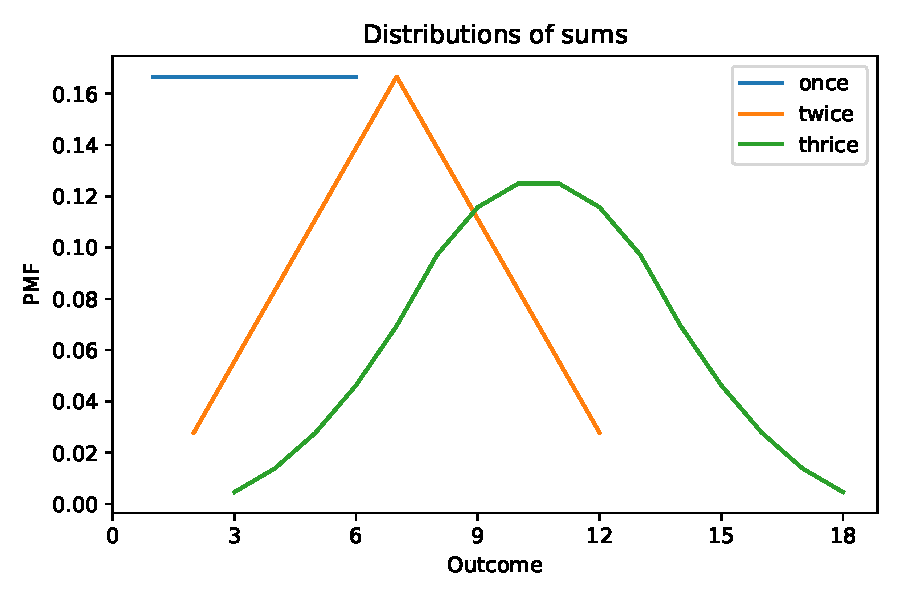
\includegraphics[width=4in]{figs/fig05-01.pdf}}
\caption{Distribution of outcomes for one six-sided die, two dice, and three dice.}
\label{fig05-01}
\end{figure}

As an aside, this example demonstrates the Central Limit Theorem, which says that the distribution of a sum converges on a bell-shaped normal distribution, at least under some conditions.

\section{Gluten}

In 2015 I read a paper that tested whether people diagnosed with gluten sensitivity (but not celiac disease) were not able to distinguish gluten flour from non-gluten flour in a blind challenge (\url{https://onlinelibrary.wiley.com/doi/full/10.1111/apt.13372}).

Out of 35 subjects, 12 correctly identified the gluten flour based on resumption of symptoms while they were eating it.  Another 17 wrongly identified the gluten-free flour based on their symptoms, and 6 were unable to distinguish.  

The authors conclude, ``Double-blind gluten challenge induces symptom recurrence in just one-third of patients.''

This conclusion seems odd to me, because if none of the patients were sensitive to gluten, we would expect some of them to identify the gluten flour by chance.
So here's the question: based on this data, how many of the subjects are sensitive to gluten?

We can use Bayes's Theorem to answer this question, but first we have to make some modeling decisions.
I'll assume:

\begin{itemize}

\item People who are sensitive to gluten have a 95\% chance of correctly identifying gluten flour under the challenge conditions, and 

\item People who are not sensitive have a 40\% chance of identifying the gluten flour by chance (and a 60\% chance of either choosing the other flour or failing to distinguish).

\end{itemize}

These particular values are arbitrary, but the results are not sensitive to these choices.

I will solve this problem in two steps.  First, assuming that we know how many subjects are sensitive, I will compute the distribution of the data.  Then, using the likelihood of the data, I will compute the posterior distribution of the number of sensitive patients.

The first is the {\bf forward problem}; the second is the {\bf inverse problem}.

\section{Forward problem}

Suppose we know that 10 of the 35 subjects are sensitive to gluten.  That means that 25 are not:

\begin{code}
n = 35
n_sensitive = 10
n_insensitive = n - n_sensitive
\end{code}

Each sensitive subject has a 95\% chance of identifying the gluten flour, so the number of correct identifications follows a binomial distribution with \py{p=0.95}:

\begin{code}
dist_sensitive = make_binomial(n_sensitive, 0.95)
\end{code}

And similarly for the insensitive subjects:

\begin{code}
dist_insensitive = make_binomial(n_insensitive, 0.4)
\end{code}

\py{make_binomial} returns a \py{Pmf} that represents the distribution of correct identifications.
So we can use \py{add_dist} to compute the total number of correct identifications in both groups:

\begin{code}
dist_total = Pmf.add_dist(dist_sensitive, dist_insensitive)
\end{code}

Figure~\ref{fig05-02} shows the distribution of correct identifications among sensitive and insensitive subjects, and the total.

\begin{figure}
% chap02soln.ipynb
\centerline{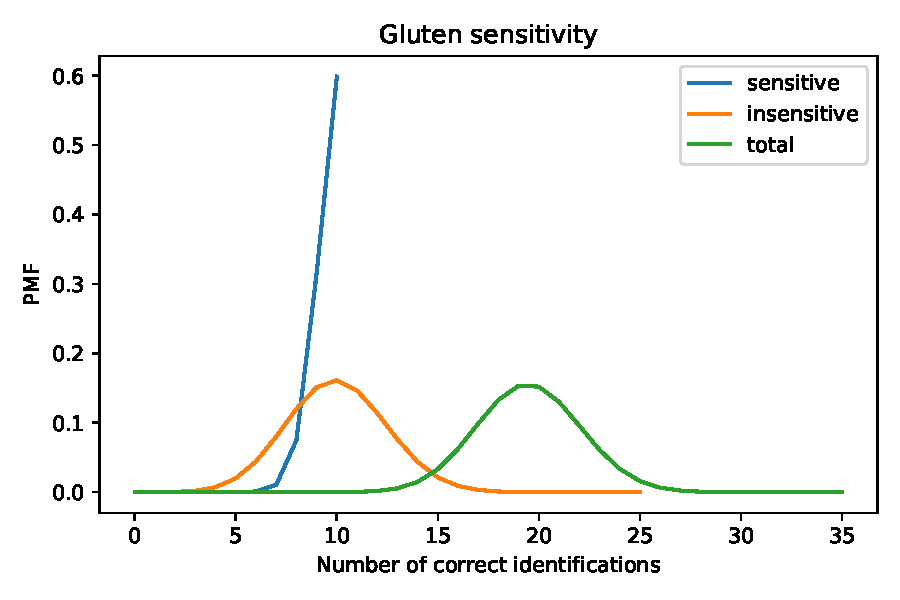
\includegraphics[width=4in]{figs/fig05-02.pdf}}
\caption{Distribution of correct identifications among sensitive and insensitive subjects, and the total.}
\label{fig05-02}
\end{figure}

Of the 10 sensitive subject, we expect most of them to identify the gluten flour correctly.
Of the 25 insensitive subjects, we expect about 10 to identify the gluten flour by chance.
So we expect about 20 correct identifications in total.

This is the answer to the forward problem: given the number of sensitive subjects, we can compute the distribution of the data.

\section{Inverse Problem}

Now let's solve the inverse problem: given the data, we'll compute the posterior distribution of the number of sensitive subjects.

Here's how.  I'll loop through the possible values of \py{n_sensitive} and compute the distribution of the data for each:

\begin{code}
table = pd.DataFrame()
for n_sensitive in range(1, n):
    n_insensitive = n - n_sensitive

    dist_sensitive = make_binomial(n_sensitive, 0.95)
    dist_insensitive = make_binomial(n_insensitive, 0.4)
    dist_total = Pmf.add_dist(dist_sensitive, dist_insensitive)    
    table[n_sensitive] = dist_total
\end{code}

I store each distribution as a column in a Pandas DataFrame.
When \py{n_sensitive} is 0 or \py{n}, the distribution of the data is a simple binomial, not the sum of two binomials:

\begin{code}
table[0] = make_binomial(n, 0.4)
table[n] = make_binomial(n, 0.95)
\end{code}

Figure~\ref{fig05-03} shows several columns from this table, corresponding to several hypothetical values of \py{n_sensitive}:

\begin{figure}
% chap05soln.ipynb
\centerline{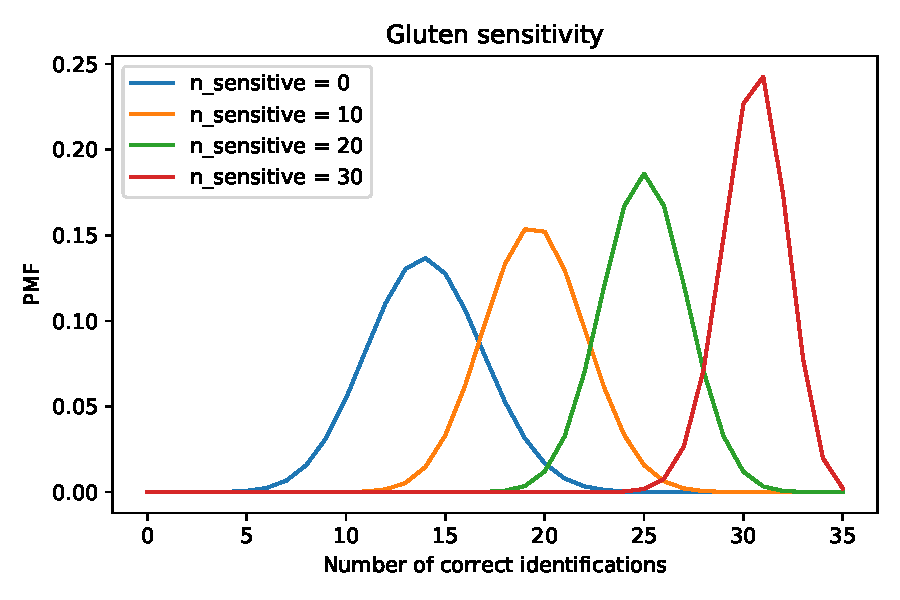
\includegraphics[width=4in]{figs/fig05-03.pdf}}
\caption{Distribution of the number of correct identification for different values of \py{n_sensitive}.}
\label{fig05-03}
\end{figure}

Now we can use this table to compute the likelihood of the data:

\begin{code}
likelihood = table.loc[12]
\end{code}

\py{loc} selects a row from the table.
The row with index 12 contains the probability of 12 correct identifications for each hypothetical value of \py{n_sensitive}.
And that's exactly the likelihood we need to do a Bayesian update.

I'll use a uniform prior, which implies that I would be equally surprised by any value of \py{n_sensitive}:

\begin{code}
hypos = np.arange(n+1)
prior = Pmf(1, hypos)
\end{code}

And here's the update:

\begin{code}
posterior = prior * likelihood
posterior.normalize()
\end{code}

Figure~\ref{fig05-04} shows posterior distributions of \py{n_sensitive} based on the actual data, 12 correct identifications, and another hypothetical outcome, 20 correct identifications.

\begin{figure}
% chap05soln.ipynb
\centerline{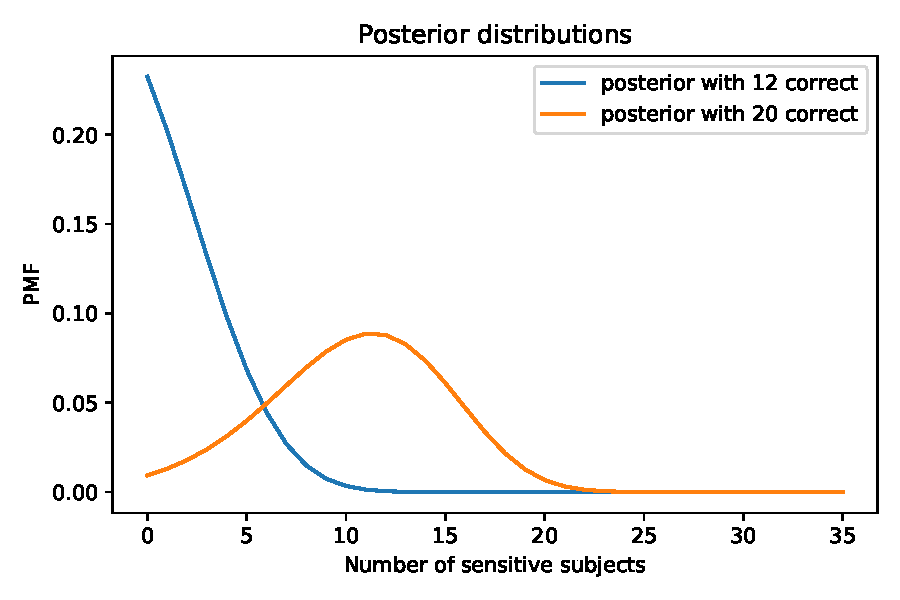
\includegraphics[width=4in]{figs/fig05-04.pdf}}
\caption{Posterior distributions of \py{n_sensitive}.}
\label{fig05-04}
\end{figure}

With 12 correct identifications, the most likely conclusion is that none of the subjects are sensitive to gluten.
If there had been 20 correct identifications, the most likely conclusion would be that 11-12 of the subjects were sensitive.


\section{Summary}

\section{Exercises}

\begin{exercise}
\end{exercise}


\begin{exercise}
\end{exercise}


\begin{exercise}
\end{exercise}


\begin{exercise}
\end{exercise}


\begin{exercise}
\end{exercise}



\chapter{Maxima and Mixtures}

\section{Maxima}

\begin{figure}
% dungeons.py
\centerline{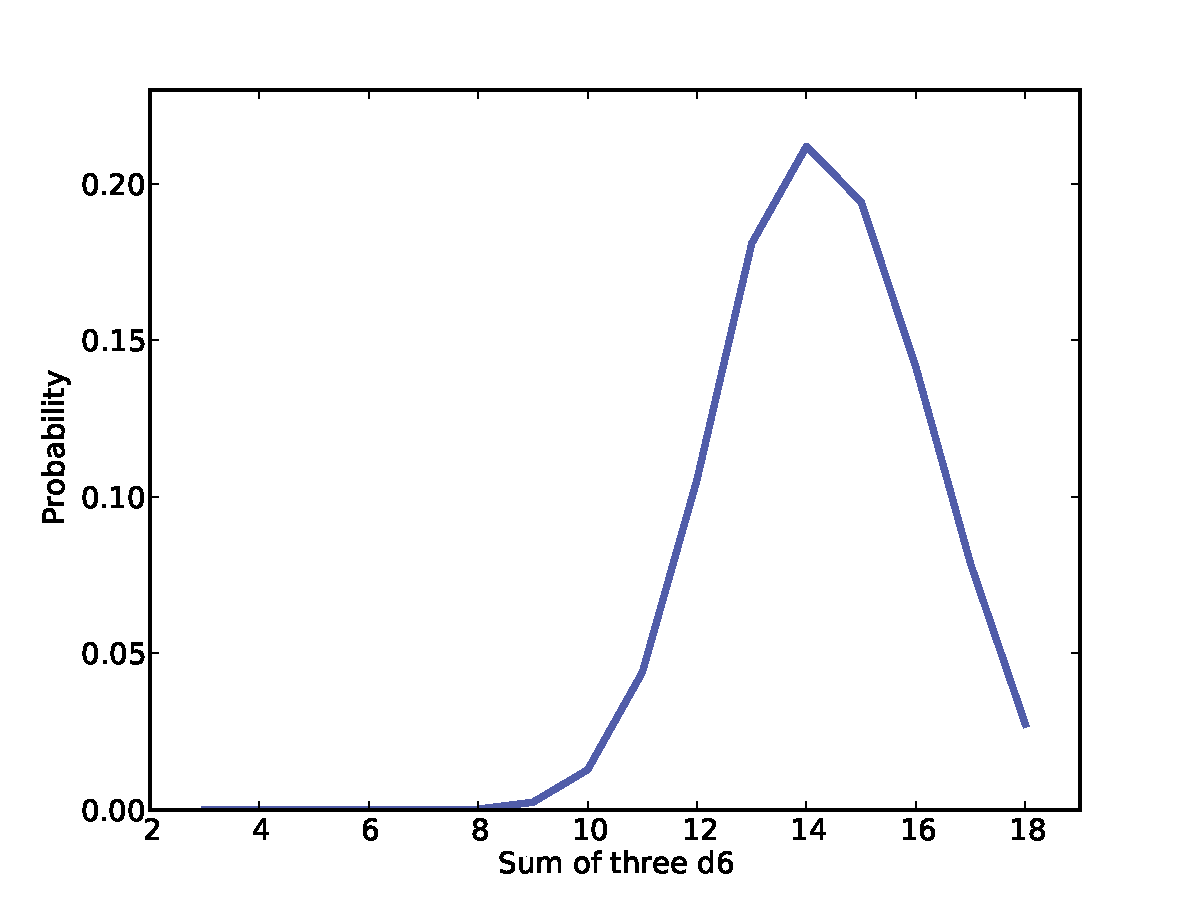
\includegraphics[height=2.5in]{figs/dungeons2.pdf}}
\caption{Distribution of the maximum of six rolls of three dice.}
\label{fig.dungeons2}
\end{figure}

When you generate a {\it Dungeons~\&~Dragons} character, you are
particularly interested in the character's best attributes, so
you might like to know the
distribution of the maximum attribute.

There are three ways to compute the distribution of a maximum:
\index{maximum}
\index{simulation}
\index{enumeration}
\index{exponentiation}

\begin{description}

\item[Simulation:] Given a Pmf that represents the distribution
for a single selection, you can generate random samples, find the maximum,
and accumulate the distribution of simulated maxima.

\item[Enumeration:] Given two Pmfs, you can enumerate all possible
pairs of values and compute the distribution of the maximum.

\item[Exponentiation:] If we convert a Pmf to a Cdf, there is a simple
and efficient algorithm for finding the Cdf of the maximum.

\end{description}

The code to simulate maxima is almost identical to the code for
simulating sums:

\begin{code}
def RandomMax(dists):
    total = max(dist.Random() for dist in dists)
    return total

def SampleMax(dists, n):
    pmf = MakePmfFromList(RandomMax(dists) for i in xrange(n))
    return pmf
\end{code}

All I did was replace ``sum'' with ``max''.  And the code
for enumeration is almost identical, too:

\begin{code}
def PmfMax(pmf1, pmf2):
    res = thinkbayes.Pmf()
    for v1, p1 in pmf1.Items():
        for v2, p2 in pmf2.Items():
            res.Incr(max(v1, v2), p1*p2)
    return res
\end{code}

In fact, you could generalize this function by taking the
appropriate operator as a parameter.

The only problem with this algorithm is that if each Pmf
has $m$ values, the run time is proportional to $m^2$.
And if we want the maximum of {\tt k} selections, it takes
time proportional to $k m^2$.

If we convert the Pmfs to Cdfs, we can do the same calculation
much faster!  The key is to remember the definition of the
cumulative distribution function:
%
\[ CDF(x) = \p{X \le~x} \]
%
where $X$ is a random variable that means ``a value chosen
randomly from this distribution.''  So, for example, $CDF(5)$
is the probability that a value from this distribution is less
than or equal to 5.

If I draw $X$ from $CDF_1$ and $Y$ from $CDF_2$, and compute
the maximum $Z = max(X, Y)$, what is the chance that $Z$ is
less than or equal to 5?  Well, in that case both $X$ and $Y$
must be less than or equal to 5.

\index{independence}
If the selections of $X$ and $Y$ are independent,
%
\[ CDF_3(5) = CDF_1(5) CDF_2(5) \] 
%
where $CDF_3$ is the distribution of $Z$.  I chose the value
5 because I think it makes the formulas easy to read, but we
can generalize for any value of $z$:
%
\[ CDF_3(z) = CDF_1(z) CDF_2(z) \]
%
In the special case where we draw $k$ values from the same
distribution, 
%
\[ CDF_k(z) = CDF_1(z)^k \]
%
So to find the distribution of the maximum of $k$ values,
we can enumerate the probabilities in the given Cdf
and raise them to the $k$th power.
\verb"Cdf" provides a method that does just that:

\begin{code}
# class Cdf

    def Max(self, k):
        cdf = self.Copy()
        cdf.ps = [p**k for p in cdf.ps]
        return cdf
\end{code}

\verb"Max" takes the number of selections, {\tt k}, and returns a new
Cdf that represents the distribution of the maximum of {\tt k}
selections.  The run time for this method is proportional to 
$m$, the number of items in the Cdf.

\verb"Pmf.Max" does the same thing for Pmfs.  It has to do a little
more work to convert the Pmf to a Cdf, so the run time is proportional
to $m \log m$, but that's still better than quadratic.

Finally, here's an example that computes the distribution of
a character's best attribute:

\begin{code}
    best_attr_cdf = three_exact.Max(6)
    best_attr_pmf = best_attr_cdf.MakePmf()
\end{code}

Where \verb"three_exact" is defined in the previous section.
If we print the results, we see that the chance of generating
a character with at least one attribute of 18 is about 3\%.
Figure~\ref{fig.dungeons2} shows the distribution.


\section{Mixtures}
\label{mixture}

\begin{figure}
% dungeons.py
\centerline{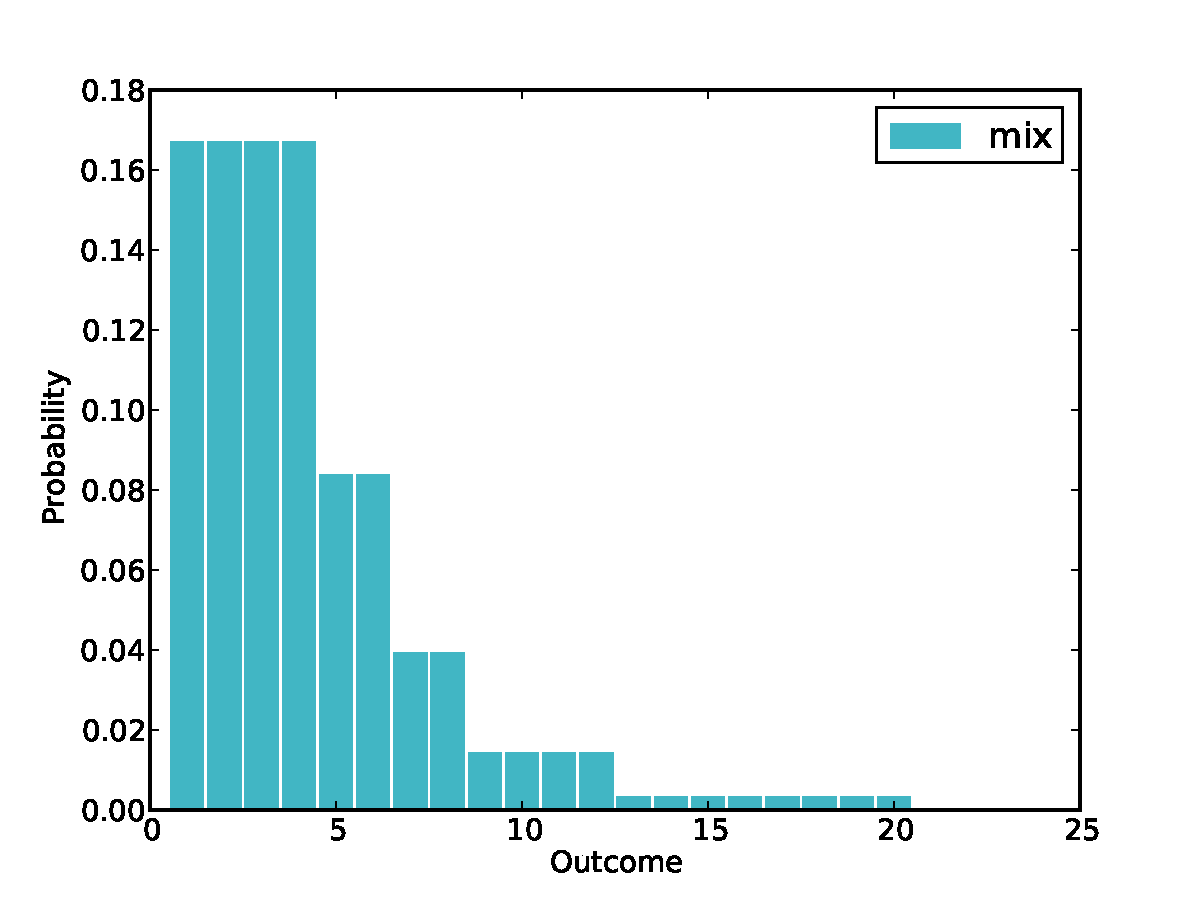
\includegraphics[height=2.5in]{figs/dungeons3.pdf}}
\caption{Distribution outcome for random die from a box.}
\label{fig.dungeons3}
\end{figure}

Let's do one more example from {\it Dungeons~\&~Dragons}.  Suppose
I have a box of dice with the following inventory:

\begin{code}
5   4-sided dice
4   6-sided dice
3   8-sided dice
2  12-sided dice
1  20-sided die
\end{code}

I choose a die from the box and roll it.  What is the distribution
of the outcome?

If you know which die it is, the answer is easy.  A die with {\tt n}
sides yields a uniform distribution from 1 to {\tt n}, including both.
\index{uniform distribution}

But if we don't know which die it is, the resulting distribution is
a {\bf mixture} of uniform distributions with different bounds.
In general, this kind of mixture does not fit any simple mathematical
model, but it is straightforward to compute the distribution in
the form of a PMF.
\index{mixture}

As always, one option is to simulate the scenario, generate a random
sample, and compute the PMF of the sample.  This approach is simple
and it generates an approximate solution quickly.  But if we want an
exact solution, we need a different approach.
\index{simulation}

Let's start with a simple version of the problem where there are
only two dice, one with 6 sides and one with 8.  We can make a Pmf to
represent each die:

\begin{code}
    d6 = Die(6)
    d8 = Die(8)
\end{code}

Then we create a Pmf to represent the mixture:

\begin{code}
    mix = thinkbayes.Pmf()
    for die in [d6, d8]:
        for outcome, prob in die.Items():
            mix.Incr(outcome, prob)
    mix.Normalize()
\end{code}

The first loop enumerates the dice; the second enumerates the
outcomes and their probabilities.  Inside the loop,
{\tt Pmf.Incr} adds up the contributions from the two distributions.

This code assumes that the two dice are equally likely.  More
generally, we need to know the probability of each die so we can
weight the outcomes accordingly.

First we create a Pmf that maps from each die to the probability it is
selected:

\begin{code}
    pmf_dice = thinkbayes.Pmf()
    pmf_dice.Set(Die(4), 5)
    pmf_dice.Set(Die(6), 4)
    pmf_dice.Set(Die(8), 3)
    pmf_dice.Set(Die(12), 2)
    pmf_dice.Set(Die(20), 1)
    pmf_dice.Normalize()
\end{code}

Next we need a more general version of the mixture algorithm:

\begin{code}
    mix = thinkbayes.Pmf()
    for die, weight in pmf_dice.Items():
        for outcome, prob in die.Items():
            mix.Incr(outcome, weight*prob)
\end{code}

Now each die has a weight associated with it (which makes it a
weighted die, I suppose).  When we add each outcome to the mixture,
its probability is multiplied by {\tt weight}.

Figure~\ref{fig.dungeons3} shows the result.  As expected, values 1
through 4 are the most likely because any die can produce them.
Values above 12 are unlikely because there is only one die in the box
that can produce them (and it does so less than half the time).

{\tt thinkbayes} provides a function named {\tt MakeMixture}
that encapsulates this algorithm, so we could have written:

\begin{code}
    mix = thinkbayes.MakeMixture(pmf_dice)
\end{code}

We'll use {\tt MakeMixture} again in Chapters~\ref{prediction} and
~\ref{observer}.


\section{Discussion}

Other than the odds form of Bayes's theorem, this chapter is not
specifically Bayesian.  But Bayesian analysis is all about
distributions, so it is important to understand the concept of a
distribution well.  From a computational point of view, a distribution
is any data structure that represents a set of values (possible
outcomes of a random process) and their probabilities.
\index{distribution}

We have seen two representations of distributions: Pmfs and Cdfs.
These representations are equivalent in the sense that they contain
the same information, so you can convert from one to the other.  The
primary difference between them is performance: some operations are
faster and easier with a Pmf; others are faster with a Cdf.
\index{Pmf} \index{Cdf}

The other goal of this chapter is to introduce operations that act on
distributions, like \verb"Pmf.__add__", {\tt Cdf.Max}, and {\tt
  thinkbayes.MakeMixture}.  We will use these operations later, but I
introduce them now to encourage you to think of a distribution as a
fundamental unit of computation, not just a container for values and
probabilities.

\section{Exercises}

\begin{exercise}
Poincare bread problem?
\end{exercise}


\begin{exercise}
\end{exercise}


\begin{exercise}
\end{exercise}


\begin{exercise}
\end{exercise}




\chapter{Prediction}
\label{prediction}

\section{The Boston Bruins problem}

In the 2010-11 National Hockey League (NHL) Finals, my beloved Boston
Bruins played a best-of-seven championship series against the despised
Vancouver Canucks.  Boston lost the first two games 0-1 and 2-3, then
won the next two games 8-1 and 4-0.  At this point in the series, what
is the probability that Boston will win the next game, and what is
their probability of winning the championship?
\index{hockey}
\index{Boston Bruins}
\index{Vancouver Canucks}

As always, to answer a question like this, we need to make some
assumptions.  First, it is reasonable to believe that goal scoring in
hockey is at least approximately a Poisson process, which means that
it is equally likely for a goal to be scored at any time during a
game.  Second, we can assume that against a particular opponent, each team
has some long-term average goals per game, denoted $\lambda$.
\index{Poisson process}

Given these assumptions, my strategy for answering this question is

\begin{enumerate}

\item Use statistics from previous games to choose a prior
distribution for $\lambda$.

\item Use the score from the first four games to estimate $\lambda$
for each team.

\item Use the posterior distributions of $\lambda$ to compute 
distribution of goals for each team, the distribution of the
goal differential, and the probability that each team wins
the next game.

\item Compute the probability that each team wins the series.

\end{enumerate}

To choose a prior distribution, I got some statistics from
\url{http://www.nhl.com}, specifically the average goals per game
for each team in the 2010-11 season.  The distribution is roughly
Gaussian with mean 2.8 and standard deviation 0.3.
\index{National Hockey League}
\index{NHL}

The Gaussian distribution is continuous, but we'll approximate it with
a discrete Pmf.  \verb"thinkbayes" provides \verb"MakeGaussianPmf" to
do exactly that:
\index{numpy}
\index{Gaussian distribution}

\begin{code}
def MakeGaussianPmf(mu, sigma, num_sigmas, n=101):
    pmf = Pmf()
    low = mu - num_sigmas*sigma
    high = mu + num_sigmas*sigma

    for x in numpy.linspace(low, high, n):
        p = scipy.stats.norm.pdf(x, mu, sigma)
        pmf.Set(x, p)
    pmf.Normalize()
    return pmf
\end{code}  

{\tt mu} and {\tt sigma} are the mean and standard deviation of the
Gaussian distribution.  \verb"num_sigmas" is the number of standard
deviations above and below the mean that the Pmf will span, and {\tt
  n} is the number of values in the Pmf.

Again we use {\tt numpy.linspace} to make an array of {\tt n}
equally spaced values between {\tt low} and {\tt high}, including
both.

\verb"norm.pdf" evaluates the Gaussian probability density function (PDF).
\index{PDF}
\index{probability density function}

Getting back to the hockey problem, here's the definition for a suite
of hypotheses about the value of $\lambda$.

\begin{code}
class Hockey(thinkbayes.Suite):

    def __init__(self):
        pmf = thinkbayes.MakeGaussianPmf(2.7, 0.3, 4)
        thinkbayes.Suite.__init__(self, pmf)
\end{code}  

So the prior distribution is Gaussian with mean 2.7, standard deviation
0.3, and it spans 4 sigmas above and below the mean.

As always, we have to decide how to represent each hypothesis; in
this case I represent the hypothesis that $\lambda=x$ with the
floating-point value {\tt x}. 


\section{Poisson processes}

In mathematical statistics, a {\bf process} is a stochastic model of a
physical system (``stochastic'' means that the model has some kind of
randomness in it).  For example, a Bernoulli process is a model of a
sequence of events, called trials, in which each trial has two
possible outcomes, like success and failure.  So a Bernoulli process
is a natural model for a series of coin flips, or a series of shots on
goal.  \index{process} \index{Poisson process}

A Poisson process is the continuous version of a Bernoulli process,
where an event can occur at any point in time with equal probability.
Poisson processes can be used to model customers arriving in a store,
buses arriving at a bus stop, or goals scored in a hockey game.
\index{Bernoulli process}

In many real systems the probability of an event changes over time.
Customers are more likely to go to a store at certain times of day,
buses are supposed to arrive at fixed intervals, and goals are more
or less likely at different times during a game.

But all models are based on simplifications, and in this case modeling
a hockey game with a Poisson process is a reasonable choice.  Heuer,
M\"{u}ller and Rubner (2010) analyze scoring in a German soccer league
and come to the same conclusion; see
\url{http://www.cimat.mx/Eventos/vpec10/img/poisson.pdf}.
\index{Heuer, Andreas}

The benefit of using this model is that we can compute the distribution
of goals per game efficiently, as well as the distribution of time
between goals.  Specifically, if the average number of goals
in a game is {\tt lam}, the distribution of goals per game is
given by the Poisson PMF:
\index{Poisson distribution}

\begin{code}
def EvalPoissonPmf(k, lam):
    return (lam)**k * math.exp(-lam) / math.factorial(k)
\end{code}  

And the distribution of time between goals is given by the
exponential PDF:
\index{exponential distribution}

\begin{code}
def EvalExponentialPdf(x, lam):
    return lam * math.exp(-lam * x)
\end{code}  

I use the variable
{\tt lam} because {\tt lambda} is a reserved keyword in Python.
Both of these functions are in \verb"thinkbayes.py".


\section{The posteriors}

\begin{figure}
% hockey.py
\centerline{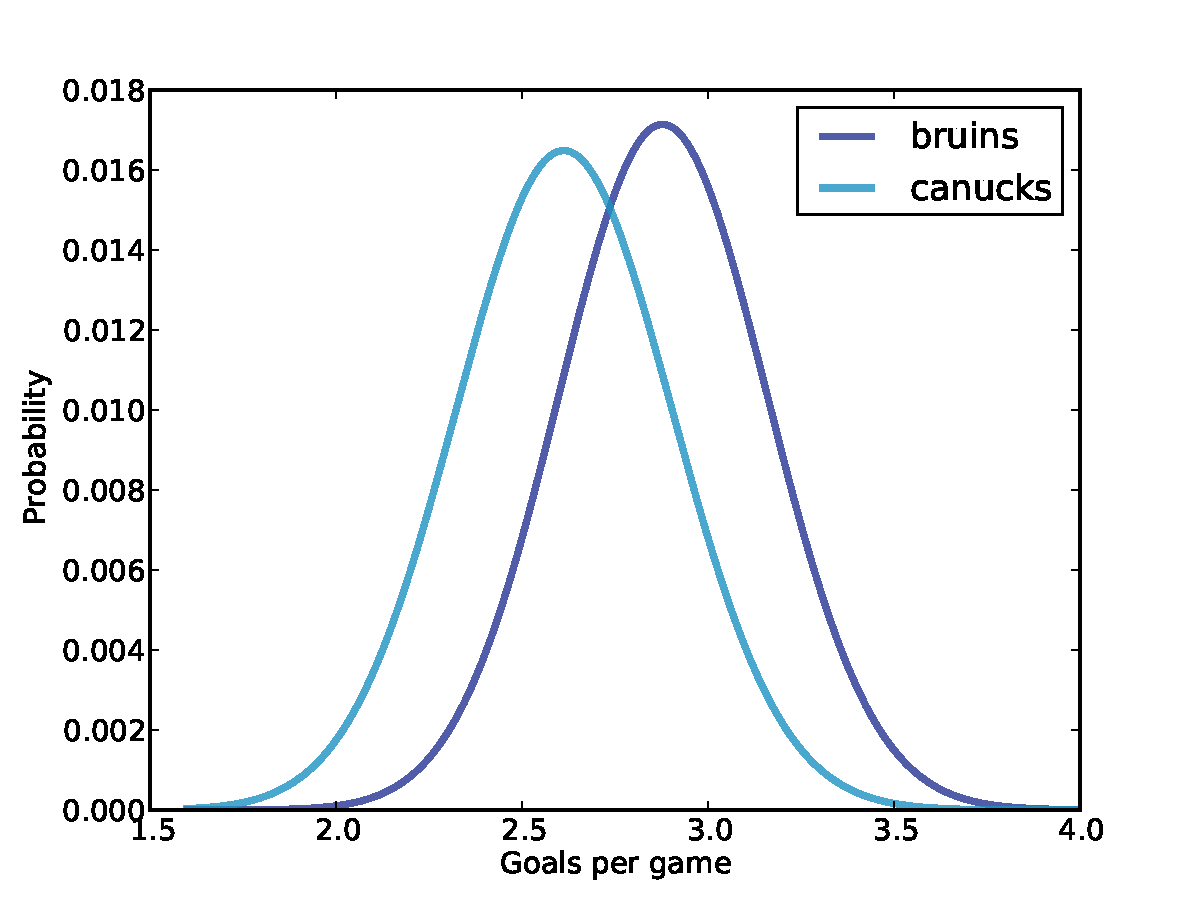
\includegraphics[height=2.5in]{figs/hockey1.pdf}}
\caption{Posterior distribution of the number of
goals per game.}
\label{fig.hockey1}
\end{figure}

Now we can compute the likelihood that a team with a hypothetical
value of {\tt lam} scores {\tt k} goals in a game:

\begin{code}
# class Hockey

    def Likelihood(self, data, hypo):
        lam = hypo
        k = data
        like = thinkbayes.EvalPoissonPmf(k, lam)
        return like
\end{code}

Each hypothesis is a possible value of $\lambda$;  {\tt
  data} is the observed number of goals, {\tt k}.

With the likelihood function in place, we can make a suite for each
team and update them with the scores from the first four games.

\begin{code}
    suite1 = Hockey('bruins')
    suite1.UpdateSet([0, 2, 8, 4])
     
    suite2 = Hockey('canucks')
    suite2.UpdateSet([1, 3, 1, 0])
\end{code}  

Figure~\ref{fig.hockey1} shows the resulting posterior distributions
for {\tt lam}.  Based on the first four games, the most likely
values for {\tt lam} are 2.6 for the Canucks and 2.9 for the Bruins.


\section{The distribution of goals}

\begin{figure}
% hockey.py
\centerline{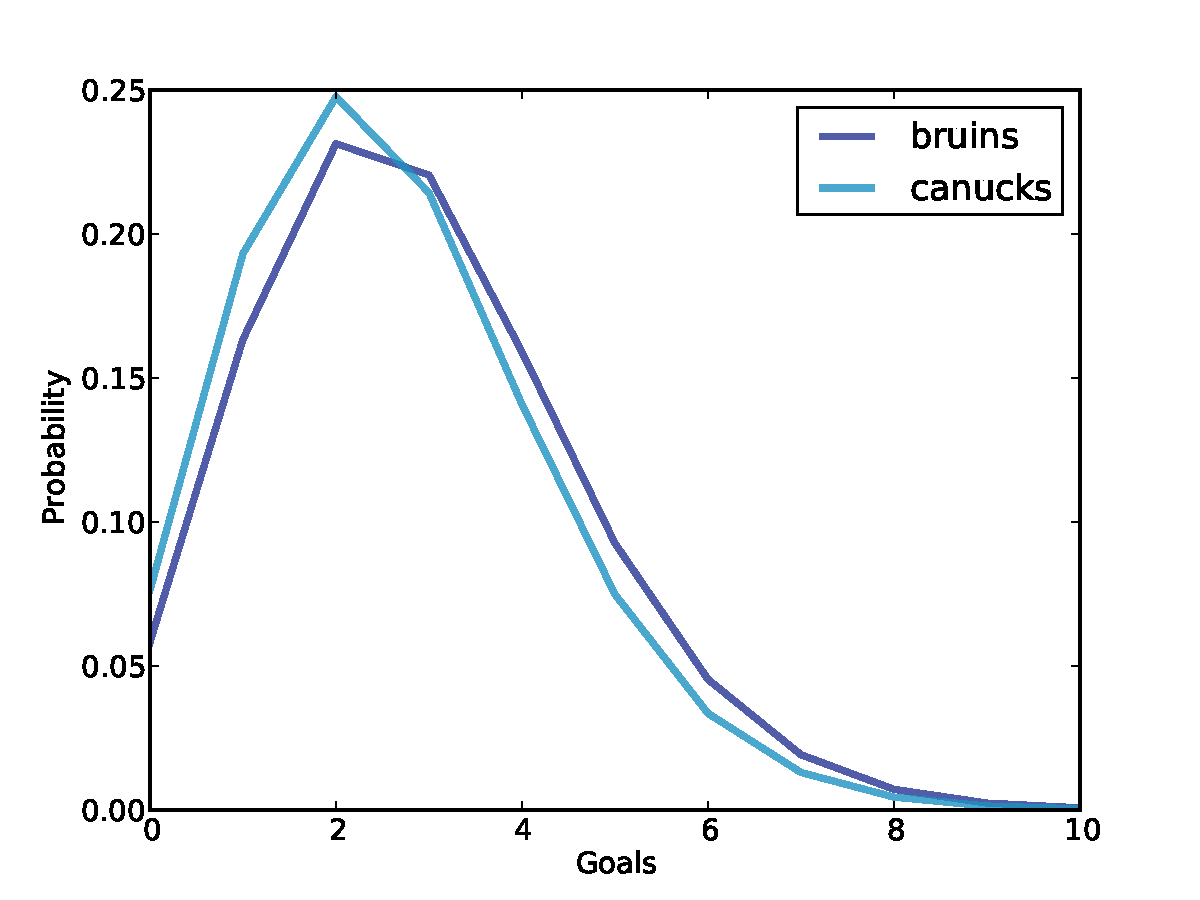
\includegraphics[height=2.5in]{figs/hockey2.pdf}}
\caption{Distribution of goals in a single game.}
\label{fig.hockey2}
\end{figure}

To compute the probability that each team wins the next game,
we need to compute the distribution of goals for each team.

If we knew the value of {\tt lam} exactly, we could use the
Poisson distribution again.  \verb"thinkbayes" provides a
method that computes a truncated approximation of a Poisson
distribution:
\index{Poisson distribution}

\begin{code}
def MakePoissonPmf(lam, high):
    pmf = Pmf()
    for k in xrange(0, high+1):
        p = EvalPoissonPmf(k, lam)
        pmf.Set(k, p)
    pmf.Normalize()
    return pmf
\end{code}  

The range of values in the computed Pmf is from 0 to {\tt high}.
So if the value of {\tt lam} were exactly 3.4, we would compute:

\begin{code}
lam = 3.4
goal_dist = thinkbayes.MakePoissonPmf(lam, 10)
\end{code}

I chose the upper bound, 10, because the probability of scoring
more than 10 goals in a game is quite low.

That's simple enough so far; the problem is that we don't know
the value of {\tt lam} exactly.  Instead, we have a distribution
of possible values for {\tt lam}.

For each value of {\tt lam}, the distribution of goals is Poisson.
So the overall distribution of goals is a mixture of these
Poisson distributions, weighted according to the probabilities
in the distribution of {\tt lam}.
\index{mixture}
\index{Poisson distribution}

Given the posterior distribution of {\tt lam}, here's the code
that makes the distribution of goals:

\begin{code}
def MakeGoalPmf(suite):
    metapmf = thinkbayes.Pmf()

    for lam, prob in suite.Items():
        pmf = thinkbayes.MakePoissonPmf(lam, 10)
        metapmf.Set(pmf, prob)

    mix = thinkbayes.MakeMixture(metapmf)
    return mix
\end{code}  

For each value of {\tt lam} we make a Poisson Pmf and add it to the
meta-Pmf.  I call it a meta-Pmf because it is a Pmf that contains
Pmfs as its values.
\index{meta-Pmf}

Then we use \verb"MakeMixture" to compute the mixture
(we saw {\tt MakeMixture} in Section~\ref{mixture}).
\index{mixture}
\index{MakeMixture}

Figure~\ref{fig.hockey2} shows the resulting distribution of goals for
the Bruins and Canucks.  The Bruins are less likely to
score 3 goals or fewer in the next game, and more likely to score 4 or
more.


\section{The probability of winning}

\begin{figure}
% hockey.py
\centerline{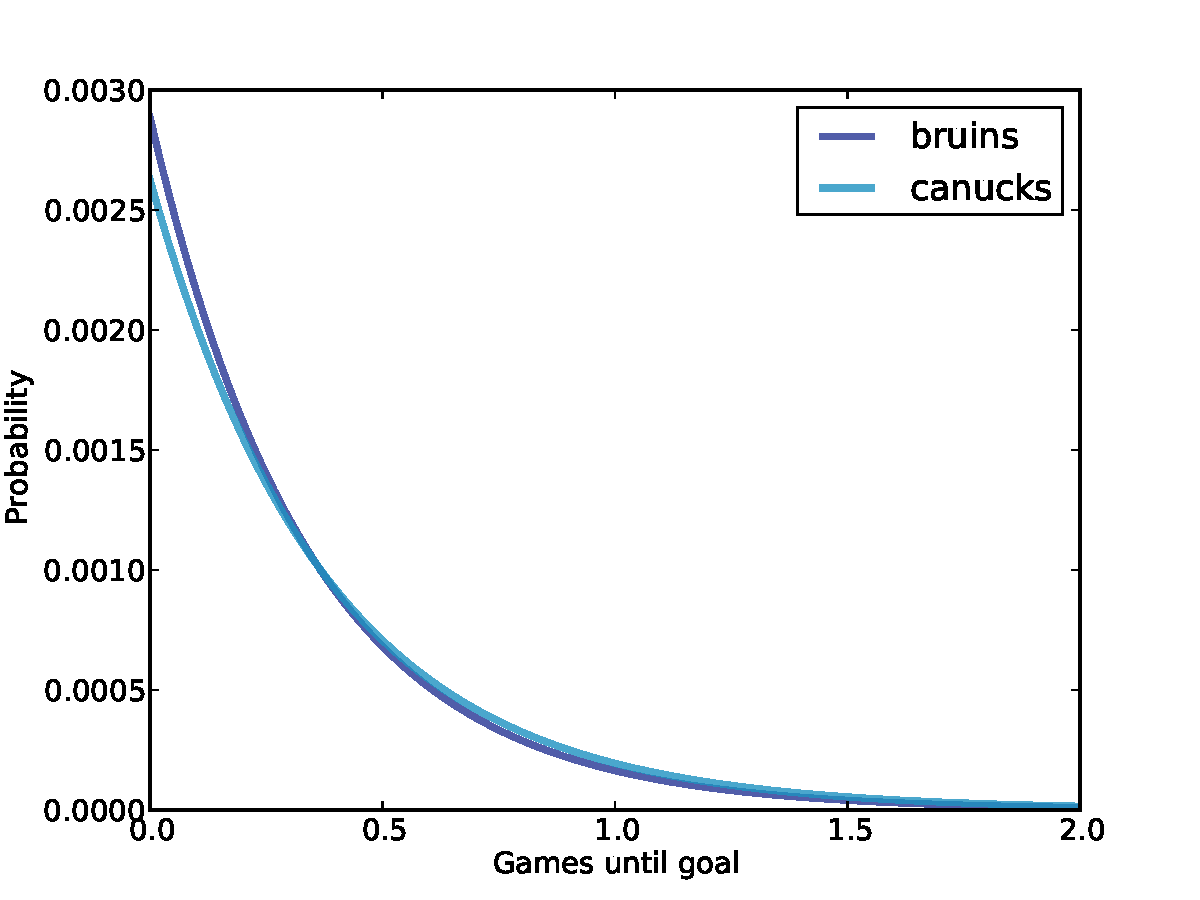
\includegraphics[height=2.5in]{figs/hockey3.pdf}}
\caption{Distribution of time between goals.}
\label{fig.hockey3}
\end{figure}

To get the probability of winning, first we compute the
distribution of the goal differential:

\begin{code}
    goal_dist1 = MakeGoalPmf(suite1)
    goal_dist2 = MakeGoalPmf(suite2)
    diff = goal_dist1 - goal_dist2
\end{code}  

The subtraction operator invokes \verb"Pmf.__sub__", which enumerates
pairs of values and computes the difference.  Subtracting two
distributions is almost the same as adding, which we saw in
Section~\ref{addends}.

If the goal differential is positive, the Bruins win; if negative, the
Canucks win; if 0, it's a tie:

\begin{code}
    p_win = diff.ProbGreater(0)
    p_loss = diff.ProbLess(0)
    p_tie = diff.Prob(0)
\end{code}  

With the distributions from the previous section, \verb"p_win"
is 46\%, \verb"p_loss" is 37\%, and \verb"p_tie" is 17\%.

In the event of a tie at the end of ``regulation play,'' the teams play
overtime periods until one team scores.  Since the game ends
immediately when the first goal is scored, this overtime format
is known as ``sudden death.''
\index{overtime}
\index{sudden death}


\section{Sudden Death}

To compute the probability of winning in a sudden death overtime,
the important statistic is not goals per game, but time until the
first goal.  The assumption that goal-scoring is a Poisson process
implies that the time between goals
is exponentially distributed.
\index{Poisson process}
\index{exponential distribution}

Given {\tt lam}, we can compute the time between goals like this: 

\begin{code}
lam = 3.4
time_dist = thinkbayes.MakeExponentialPmf(lam, high=2, n=101)
\end{code}  

{\tt high} is the upper bound of the distribution.  In this case
I chose 2, because the probability of going more than two games
without scoring is small.  {\tt n} is the number of values in
the Pmf.

If we know {\tt lam} exactly, that's all there is to it.
But we don't; instead we have a posterior
distribution of possible values.  So as we did with the distribution
of goals, we make a meta-Pmf and compute a mixture of
Pmfs.
\index{MakeMixture}
\index{meta-Pmf}
\index{mixture}

\begin{code}
def MakeGoalTimePmf(suite):
    metapmf = thinkbayes.Pmf()

    for lam, prob in suite.Items():
        pmf = thinkbayes.MakeExponentialPmf(lam, high=2, n=2001)
        metapmf.Set(pmf, prob)

    mix = thinkbayes.MakeMixture(metapmf)
    return mix
\end{code}  

Figure~\ref{fig.hockey3} shows the resulting distributions.  For
time values less than one period (one third of a game), the Bruins
are more likely to score.  The time until the Canucks score is
more likely to be longer.

I set the number of values, {\tt n}, fairly high in order to minimize
the number of ties, since it is not possible for both teams
to score simultaneously.

Now we compute the probability that the Bruins score first:

\begin{code}
    time_dist1 = MakeGoalTimePmf(suite1)
    time_dist2 = MakeGoalTimePmf(suite2)
    p_overtime = thinkbayes.PmfProbLess(time_dist1, time_dist2)
\end{code}  

For the Bruins, the probability of winning in overtime is 52\%.

Finally, the total probability of winning is the chance of
winning at the end of regulation play plus the probability
of winning in overtime.

\begin{code}
    p_tie = diff.Prob(0)
    p_overtime = thinkbayes.PmfProbLess(time_dist1, time_dist2)

    p_win = diff.ProbGreater(0) + p_tie * p_overtime
\end{code}  

For the Bruins, the overall chance of winning the next game is 55\%.

To win the series, the Bruins can either win the next two games
or split the next two and win the third.  Again, we can compute
the total probability:

\begin{code}
    # win the next two
    p_series = p_win**2

    # split the next two, win the third
    p_series += 2 * p_win * (1-p_win) * p_win
\end{code}  

The Bruins chance of winning the series is 57\%.  And in 2011,
they did.


\section{Discussion}

As always, the analysis in this chapter is based on modeling decisions,
and modeling is almost always an iterative process.  In general,
you want to start with something simple that yields an approximate
answer, identify likely sources of error, and look for opportunities
for improvement.
\index{modeling}
\index{iterative modeling}

In this example, I would consider these options:

\begin{itemize}

\item I chose a prior based on the average goals per game for each
  team.  But this statistic is averaged across all opponents.  Against
  a particular opponent, we might expect more variability.  For
  example, if the team with the best offense plays the team with the
  worst defense, the expected goals per game might be several standard
  deviations above the mean.

\item For data I used only the first four games of the championship
  series.  If the same teams played each other during the
  regular season, I could use the results from those games as well.
  One complication is that the composition of teams changes during
  the season due to trades and injuries.  So it might be best to
  give more weight to recent games.

\item To take advantage of all available information, we could
  use results from all regular season games to estimate each team's
  goal scoring rate, possibly adjusted by estimating
  an additional factor for each pairwise match-up.  This approach
  would be more complicated, but it is still feasible.

\end{itemize}

For the first option, we could use the results from the regular season
to estimate the variability across all pairwise match-ups.  Thanks to
Dirk Hoag at \url{http://forechecker.blogspot.com/}, I was able to get
the number of goals scored during regulation play (not overtime) for
each game in the regular season.
\index{Hoag, Dirk}

Teams in different conferences only play each other one or two
times in the regular season, so I focused on pairs that played
each other 4--6 times.  For each pair, I computed the average
goals per game, which is an estimate of $\lambda$, then plotted
the distribution of these estimates.

The mean of these estimates is 2.8, again, but the standard
deviation is 0.85, substantially higher than what we got computing
one estimate for each team.

If we run the analysis again with the higher-variance prior, the
probability that the Bruins win the series is 80\%, substantially
higher than the result with the low-variance prior, 57\%.

So it turns out that the results are sensitive to the prior, which
makes sense considering how little data we have to work with.  Based
on the difference between the low-variance model and the high-variable
model, it seems worthwhile to put some effort into getting the prior
right.

The code and data for this chapter are available from
\url{http://thinkbayes.com/hockey.py} and
\url{http://thinkbayes.com/hockey_data.csv}.
  For more information
see Section~\ref{download}.

\section{Exercises}

\begin{exercise}

If buses arrive at a bus stop every 20 minutes, and you
arrive at the bus stop at a random time, your wait time until
the bus arrives is uniformly distributed from 0 to 20 minutes.
\index{bus stop problem}

But in reality, there is variability in the time between
buses.  Suppose you are waiting for a bus, and you know the historical
distribution of time between buses.  Compute your distribution
of wait times.

Hint: Suppose that the time between buses is either
5 or 10 minutes with equal probability.  What is the probability
that you arrive during one of the 10 minute intervals?

I solve a version of this problem in the next chapter.

\end{exercise}


\begin{exercise}

Suppose that passengers arriving at the bus stop are well-modeled
by a Poisson process with parameter $\lambda$.  If you arrive at the
stop and find 3 people waiting, what is your posterior distribution
for the time since the last bus arrived.
\index{Poisson process}
\index{bus stop problem}

I solve a version of this problem in the next chapter.

\end{exercise}


\begin{exercise}

Suppose that you are an ecologist sampling the insect population in
a new environment.  You deploy 100 traps in a test area and come back
the next day to check on them.  You find that 37 traps have been
triggered, trapping an insect inside.  Once a trap triggers, it
cannot trap another insect until it has been reset.
\index{insect sampling problem}

If you reset the traps and come back in two days, how many traps
do you expect to find triggered?  Compute a posterior predictive
distribution for the number of traps.
\index{predictive distribution}

\end{exercise}


\begin{exercise}

Suppose you are the manager of an apartment building with
100 light bulbs in common areas.  It is your responsibility
to replace light bulbs when they break.
\index{light bulb problem}

On January 1, all 100 bulbs are working.  When you inspect
them on February 1, you find 3 light bulbs out.  If you
come back on April 1, how many light bulbs do you expect to
find broken?

In the previous exercise, you could reasonably assume that an event is
equally likely at any time.  For light bulbs, the likelihood of
failure depends on the age of the bulb.  Specifically, old bulbs
have an increasing failure rate due to evaporation of the filament.

This problem is more open-ended than some; you will have to make
modeling decisions.  You might want to read about the Weibull
distribution
(\url{http://en.wikipedia.org/wiki/Weibull_distribution}).
Or you might want to look around for information about
light bulb survival curves.
\index{Weibull distribution}

\end{exercise}



\chapter{Decision Analysis}
\label{decisionanalysis}

\section{The {\it Price is Right} problem}

On November 1, 2007, contestants named Letia and Nathaniel appeared
on {\it The Price is Right}, an American game show.  They competed in
a game called {\it The Showcase}, where the objective is to guess the price
of a showcase of prizes.  The contestant who comes closest to the
actual price of the showcase, without going over, wins the prizes.
\index{Price is Right}
\index{Showcase}

Nathaniel went first.  His showcase included a dishwasher, a wine
cabinet, a laptop computer, and a car.  He bid \$26,000.

Letia's showcase included a pinball machine, a video arcade game, a
pool table, and a cruise of the Bahamas.  She bid \$21,500.

The actual price of Nathaniel's showcase was \$25,347.  His bid
was too high, so he lost.

The actual price of Letia's showcase was \$21,578.  She was only
off by \$78, so she won her showcase and, because
her bid was off by less than \$250, she also won Nathaniel's
showcase.

For a Bayesian thinker, this scenario suggests several questions:

\begin{enumerate}

\item Before seeing the prizes, what prior beliefs should the
  contestant have about the price of the showcase?

\item After seeing the prizes, how should the contestant update
  those beliefs?

\item Based on the posterior distribution, what should the
  contestant bid?

\end{enumerate}

The third question demonstrates a common use of Bayesian analysis:
decision analysis.  Given a posterior distribution, we can choose
the bid that maximizes the contestant's expected return.
\index{decision analysis}

This problem is inspired by an example in Cameron Davidson-Pilon's
book, {\it Bayesian Methods for Hackers}.  The code I wrote for this
chapter is available from \url{http://thinkbayes.com/price.py}; it
reads data files you can download from
\url{http://thinkbayes.com/showcases.2011.csv} and
\url{http://thinkbayes.com/showcases.2012.csv}.    For more information
see Section~\ref{download}.
\index{Davidson-Pilon, Cameron}


\section{The prior}

\begin{figure}
% price.py
\centerline{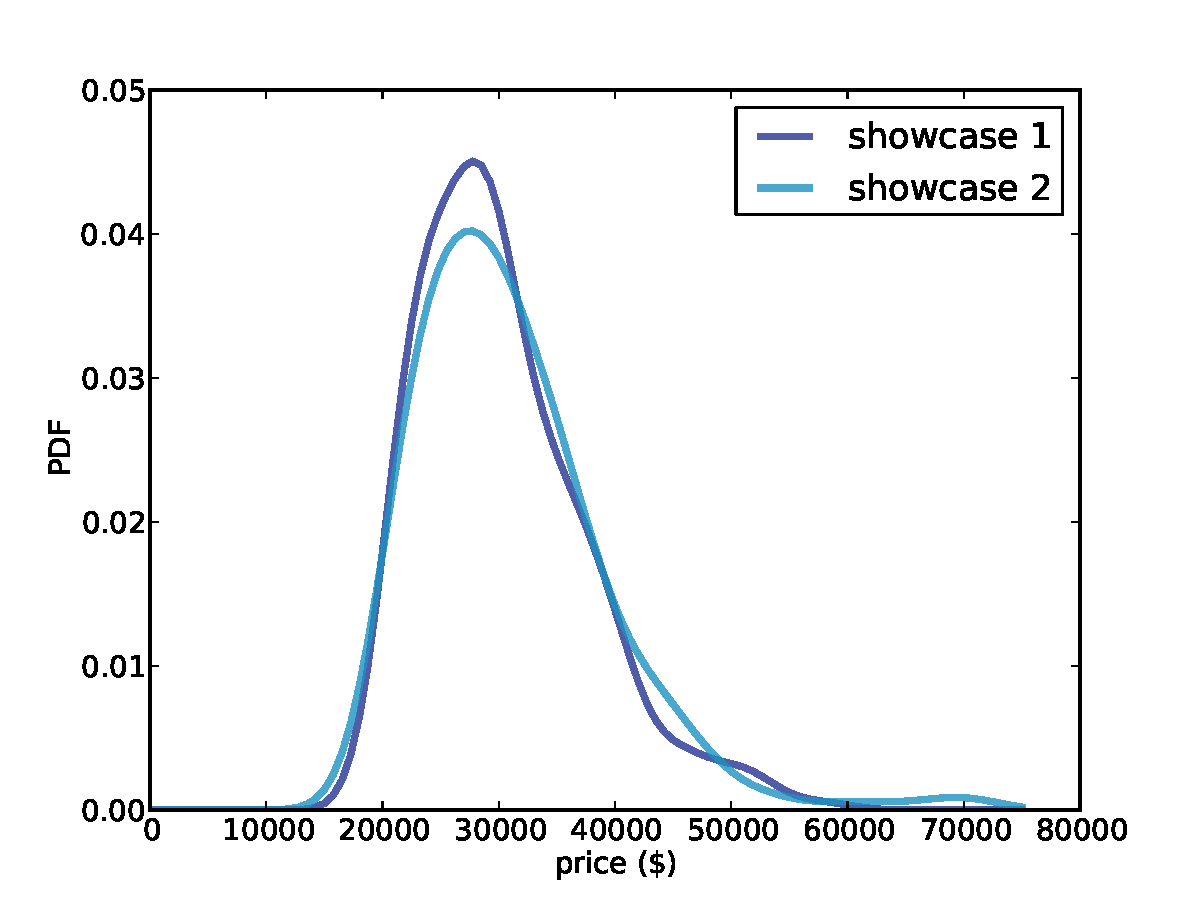
\includegraphics[height=2.5in]{figs/price1.pdf}}
\caption{Distribution of prices for showcases on
{\it The Price is Right}, 2011-12.}
\label{fig.price1}
\end{figure}

To choose a prior distribution of prices, we can take advantage
of data from previous episodes.  Fortunately, fans of the show
keep detailed records.  When I corresponded with Mr.~Davidson-Pilon
about his book, he sent me data collected by Steve Gee at
\url{http://tpirsummaries.8m.com}.  It includes the price of
each showcase from the 2011 and 2012 seasons and the bids
offered by the contestants.
\index{Gee, Steve}

Figure~\ref{fig.price1} shows the distribution of prices for these
showcases.  The most common value for both showcases is around
\$28,000, but the first showcase has a second mode near \$50,000,
and the second showcase is occasionally worth more than \$70,000.

These distributions are based on actual data, but they
have been smoothed by Gaussian kernel density estimation (KDE).
Before we go on, I want to take a detour to talk about 
probability density functions and KDE.
\index{kernel density estimation}
\index{KDE}


\section{Probability density functions}

So far we have been working with probability mass functions, or PMFs.
A PMF is a map from each possible value to its probability.  In my
implementation, a Pmf object provides a method named {\tt Prob} that
takes a value and returns a probability, also known as a {\bf probability
mass}.
\index{probability density function}
\index{Pdf}
\index{Pmf}

A {\bf probability density function}, or PDF, is the continuous version of a
PMF, where the possible values make up a continuous range rather than
a discrete set.  

\index{Gaussian distribution}
In mathematical notation, PDFs are usually written as functions; for
example, here is the PDF of a Gaussian distribution with
mean 0 and standard deviation 1:
%
\[ f(x) = \frac{1}{\sqrt{2 \pi}} \exp(-x^2/2) \]
%
For a given value of $x$, this function computes a probability
density.  
A density is similar
to a probability mass in the sense that a higher density indicates
that a value is more likely.
\index{density}
\index{probability density}
\index{probability}

But a density is not a probability.  A density can be 0 or any positive
value; it is not bounded, like a probability, between 0 and 1.

If you integrate a density
over a continuous range, the result is a probability.  But 
for the applications in this book we seldom have to do that.

Instead we primarily use probability densities as part
of a likelihood function.  We will see an example soon.


\section{Representing PDFs}

\index{Pdf}
To represent PDFs in Python,
{\tt thinkbayes.py} provides a class named {\tt Pdf}.
{\tt Pdf} is an {\bf abstract type}, which means that it defines
the interface a Pdf is supposed to have, but does not provide
a complete implementation.  The {\tt Pdf} interface includes
two methods, {\tt Density} and {\tt MakePmf}:

\begin{code}
class Pdf(object):

    def Density(self, x):
        raise UnimplementedMethodException()

    def MakePmf(self, xs):
        pmf = Pmf()
        for x in xs:
            pmf.Set(x, self.Density(x))
        pmf.Normalize()
        return pmf
\end{code}

{\tt Density} takes a value, {\tt x}, and returns the corresponding
density.  {\tt MakePmf} makes a discrete approximation to the PDF.

{\tt Pdf} provides an implementation of {\tt MakePmf}, but not {\tt
  Density}, which has to be provided by a child class.
\index{abstract type} \index{concrete type} \index{interface}
\index{implementation}

\index{Gaussian distribution}
A {\bf concrete type} is a child class that extends an abstract type
and provides an implementation of the missing methods.
For example, {\tt GaussianPdf} extends {\tt Pdf} and provides
{\tt Density}:

\begin{code}
class GaussianPdf(Pdf):

    def __init__(self, mu, sigma):
        self.mu = mu
        self.sigma = sigma
        
    def Density(self, x):
        return scipy.stats.norm.pdf(x, self.mu, self.sigma)
\end{code}

\verb"__init__" takes {\tt mu} and {\tt sigma}, which are
the mean and standard deviation of the distribution, and stores
them as attributes.

{\tt Density} uses a function from {\tt scipy.stats} to evaluate the
Gaussian PDF.  The function is called {\tt norm.pdf} because the
Gaussian distribution is also called the ``normal'' distribution. 
\index{scipy}
\index{normal distribution}

The Gaussian PDF is defined by a simple mathematical function,
so it is easy to evaluate.  And it is useful because many
quantities in the real world have distributions that are
approximately Gaussian.
\index{Gaussian distribution}
\index{Gaussian PDF}

But with real data, there is no guarantee that the distribution
is Gaussian or any other simple mathematical function.  In
that case we can use a sample to estimate the PDF of
the whole population.

For example, in {\it The Price Is Right} data, we have
313 prices for the first showcase.  We can think of these
values as a sample from the population of all possible showcase
prices.

This sample includes the following values (in order):
%
\[ 28800, 28868, 28941, 28957, 28958 \]
%
In the sample, no values appear between 28801 and 28867, but
there is no reason to think that these values are impossible.
Based on our background information, we expect all
values in this range to be equally likely.  In other words,
we expect the PDF to be fairly smooth.

Kernel density estimation (KDE) is an algorithm that takes
a sample and finds an appropriately smooth PDF that fits 
the data.  You can read details at
\url{http://en.wikipedia.org/wiki/Kernel_density_estimation}.
\index{KDE}
\index{kernel density estimation}

{\tt scipy} provides an implementation of KDE and  {\tt thinkbayes}
provides a class called {\tt EstimatedPdf} that 
uses it:
\index{scipy}
\index{numpy}

\begin{code}
class EstimatedPdf(Pdf):

    def __init__(self, sample):
        self.kde = scipy.stats.gaussian_kde(sample)

    def Density(self, x):
        return self.kde.evaluate(x)
\end{code}

\verb"__init__" takes a sample
and computes a kernel density estimate.  The result is a
\verb"gaussian_kde" object that provides an {\tt evaluate}
method.

{\tt Density} takes a value, calls \verb"gaussian_kde.evaluate",
and returns the resulting density.
\index{density}

Finally, here's an outline of the code I used to generate
Figure~\ref{fig.price1}:
\index{numpy}

\begin{code}
    prices = ReadData()
    pdf = thinkbayes.EstimatedPdf(prices)

    low, high = 0, 75000
    n = 101
    xs = numpy.linspace(low, high, n) 
    pmf = pdf.MakePmf(xs)
\end{code}

{\tt pdf} is a {\tt Pdf} object, estimated by KDE.  {\tt pmf}
is a Pmf object that approximates the Pdf by evaluating the density
at a sequence of equally spaced values.

{\tt linspace} stands for
``linear space.''  It takes a range, {\tt low} and {\tt high}, and
the number of points, {\tt n}, and returns a new {\tt numpy}
array with {\tt n} elements equally spaced between {\tt low} and
{\tt high}, including both.

And now back to {\it The Price is Right}.


\section{Modeling the contestants}

\begin{figure}
% price.py
\centerline{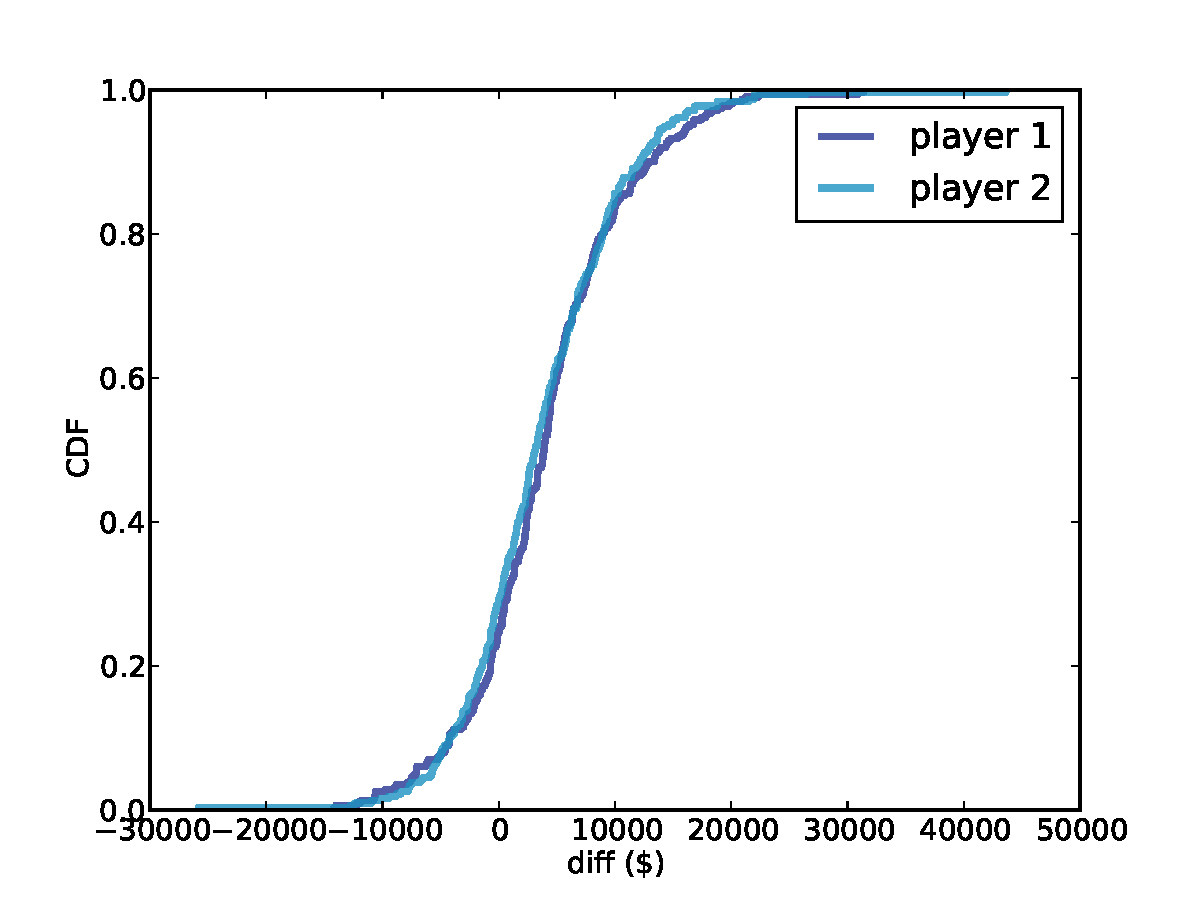
\includegraphics[height=2.5in]{figs/price2.pdf}}
\caption{Cumulative distribution (CDF) of the difference between the
  contestant's bid and the actual price.}
\label{fig.price2}
\end{figure}

The PDFs in Figure~\ref{fig.price1} estimate the distribution of
possible prices.  If you were a contestant on the
show, you could use this distribution to quantify your prior belief
about the price of each showcase (before you see the prizes).

To update these priors, we have to answer these questions:

\begin{enumerate}

\item What data should we consider and how should we quantify it?

\item Can we compute a likelihood function; that is,
  for each hypothetical value of {\tt price}, can we compute
  the conditional likelihood of the data?

\end{enumerate}

To answer these questions, I am going to model the contestant
as a price-guessing instrument with known error characteristics.
In other words, when the contestant sees the prizes, he or she
guesses the price of each prize---ideally without taking into
consideration the fact that the prize is part of a showcase---and
adds up the prices.  Let's call this total {\tt guess}.
\index{error}

Under this model, the question we have to answer is, ``If the
actual price is {\tt price}, what is the likelihood that the
contestant's estimate would be {\tt guess}?''
\index{likelihood}

Or if we define
%
\begin{code}
    error = price - guess
\end{code}
%
then we could ask, ``What is the likelihood
that the contestant's estimate is off by {\tt error}?''

To answer this question, we can use the historical data again.
Figure~\ref{fig.price2} shows the cumulative distribution of {\tt diff},
the difference between the contestant's bid and the actual price
of the showcase.
\index{Cdf}

The definition of diff is
%
\begin{code}
    diff = price - bid
\end{code}
%
When {\tt diff} is negative, the bid is too high.  As an
aside, we can use this distribution to compute the probability that the
contestants overbid: the first contestant overbids 25\% of the
time; the second contestant overbids 29\% of the time.

We can also see that the bids are biased;
that is, they are more likely to be too low than too high.  And
that makes sense, given the rules of the game.

Finally, we can use this distribution to estimate the reliability of
the contestants' guesses.  This step is a little tricky because
we don't actually know the contestant's guesses; we only know
what they bid.

So we'll have to make some assumptions.  Specifically, I
assume that the distribution of {\tt error} is Gaussian with mean 0
and the same variance as {\tt diff}.
\index{Gaussian distribution}

The {\tt Player} class implements this model:
\index{numpy}

\begin{code}
class Player(object):

    def __init__(self, prices, bids, diffs):
        self.pdf_price = thinkbayes.EstimatedPdf(prices)
        self.cdf_diff = thinkbayes.MakeCdfFromList(diffs)

        mu = 0
        sigma = numpy.std(diffs)
        self.pdf_error = thinkbayes.GaussianPdf(mu, sigma)
\end{code}

{\tt prices} is a sequence of showcase prices, {\tt bids} is a
sequence of bids, and {\tt diffs} is a sequence of diffs, where
again {\tt diff = price - bid}.

\verb"pdf_price" is the smoothed PDF of prices, estimated by KDE.
\verb"cdf_diff" is the cumulative distribution of {\tt diff},
which we saw in Figure~\ref{fig.price2}.  And \verb"pdf_error"
is the PDF that characterizes the distribution of errors; where
{\tt error = price - guess}.

Again, we use the variance of {\tt diff} to estimate the variance of
{\tt error}.  This estimate is not perfect because contestants' bids
are sometimes strategic; for example, if Player 2 thinks that Player 1
has overbid, Player 2 might make a very low bid.  In that case {\tt
  diff} does not reflect {\tt error}.  If this happens a lot, the
observed variance in {\tt diff} might overestimate the variance in
{\tt error}.  Nevertheless, I think it is a reasonable modeling
decision.

As an alternative, someone preparing to appear on the show could
estimate their own distribution of {\tt error} by watching previous shows
and recording their guesses and the actual prices.


\section{Likelihood}

Now we are ready to write the likelihood function.  As usual,
I define a new class that extends {\tt thinkbayes.Suite}:
\index{likelihood}

\begin{code}
class Price(thinkbayes.Suite):

    def __init__(self, pmf, player):
        thinkbayes.Suite.__init__(self, pmf)
        self.player = player
\end{code}

{\tt pmf} represents the prior distribution and
{\tt player} is a Player object as described in the previous
section.  Here's {\tt Likelihood}:

\begin{code}
    def Likelihood(self, data, hypo):
        price = hypo
        guess = data

        error = price - guess
        like = self.player.ErrorDensity(error)

        return like
\end{code}

{\tt hypo} is the hypothetical price of the showcase.  {\tt data}
is the contestant's best guess at the price.  {\tt error} is
the difference, and {\tt like} is the likelihood of the data,
given the hypothesis.

{\tt ErrorDensity} is defined in {\tt Player}:

\begin{code}
# class Player:

    def ErrorDensity(self, error):
        return self.pdf_error.Density(error)
\end{code}

{\tt ErrorDensity} works by evaluating \verb"pdf_error" at
the given value of {\tt error}.
The result is a probability density, so it is not really a probability.
But remember that {\tt Likelihood} doesn't
need to compute a probability; it only has to compute something {\em
  proportional} to a probability.  As long as the constant of
proportionality is the same for all likelihoods, it gets canceled out
when we normalize the posterior distribution.
\index{density}
\index{likelihood}

And therefore, a probability density is a perfectly good likelihood.


\section{Update}

\begin{figure}
% price.py
\centerline{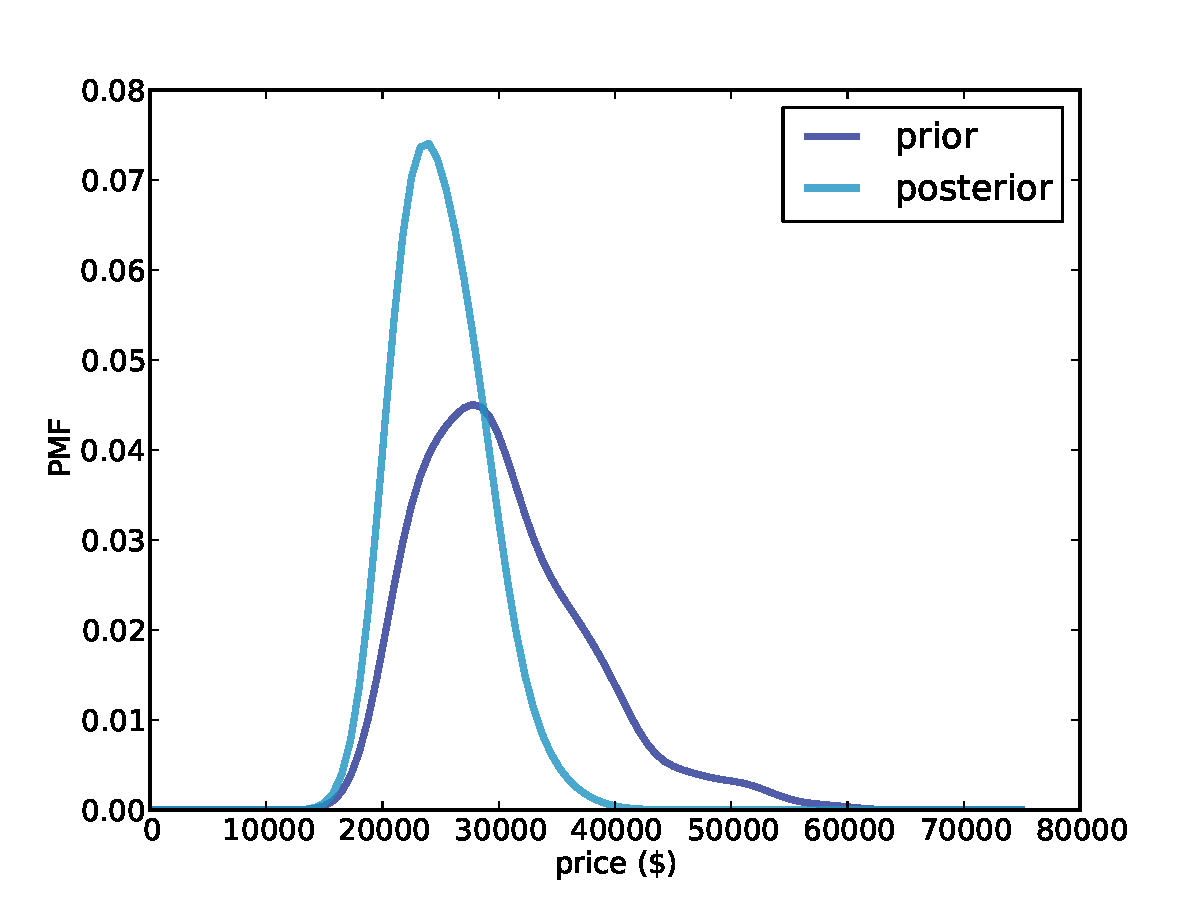
\includegraphics[height=2.5in]{figs/price3.pdf}}
\caption{Prior and posterior distributions for Player 1, based on
  a best guess of \$20,000.}
\label{fig.price3}
\end{figure}


{\tt Player} provides a method that takes the contestant's
guess and computes the posterior distribution:

\begin{code}
# class Player

    def MakeBeliefs(self, guess):
        pmf = self.PmfPrice()
        self.prior = Price(pmf, self)
        self.posterior = self.prior.Copy()
        self.posterior.Update(guess)
\end{code}

{\tt PmfPrice} generates a discrete approximation
to the PDF of price, which we use to construct the prior.

{\tt PmfPrice} uses {\tt MakePmf}, which
evaluates \verb"pdf_price" at a sequence of values:

\begin{code}
# class Player

    n = 101
    price_xs = numpy.linspace(0, 75000, n)

    def PmfPrice(self):
        return self.pdf_price.MakePmf(self.price_xs)
\end{code}

To construct the posterior, we make a copy of the
prior and then invoke {\tt Update}, which invokes {\tt Likelihood}
for each hypothesis, multiplies the priors by the likelihoods,
and  renormalizes.
\index{normalize}

So let's get back to the original scenario.  Suppose you are
Player 1 and when you see your showcase, your best guess is
that the total price of the prizes is \$20,000.

Figure~\ref{fig.price3} shows prior and
posterior beliefs about the actual price.
The posterior is shifted
to the left because your guess 
is on the low end of the prior range.

On one level, this result makes sense.  The most likely value
in the prior is \$27,750, your best guess is \$20,000, and
the mean of the posterior is somewhere in between: \$25,096.

On another level, you might find this result bizarre, because it
suggests that if you {\em think} the price is \$20,000, then you
should {\em believe} the price is \$24,000.

To resolve this apparent paradox, remember that you are combining two
sources of information, historical data about past showcases and
guesses about the prizes you see.

We are treating the historical data as the prior and updating it
based on your guesses, but we could equivalently use your guess
as a prior and update it based on historical data.  

If you think of it that way, maybe it is less surprising that the
most likely value in the posterior is not your original guess.


\section{Optimal bidding}

Now that we have a posterior distribution, we can use it to
compute the optimal bid, which I define as the bid that maximizes
expected return (see \url{http://en.wikipedia.org/wiki/Expected_return}).
\index{decision analysis}

I'm going to present the methods in this section top-down, which
means I will show you how they are used before I show you how they
work.  If you see an unfamiliar method, don't worry; the definition
will be along shortly.

To compute optimal bids, I wrote a class called {\tt GainCalculator}:

\begin{code}
class GainCalculator(object):

    def __init__(self, player, opponent):
        self.player = player
        self.opponent = opponent
\end{code}

{\tt player} and {\tt opponent} are {\tt Player} objects.

{\tt GainCalculator} provides {\tt ExpectedGains}, which
computes a sequence of bids and the expected gain for each
bid:
\index{numpy}

\begin{code}
    def ExpectedGains(self, low=0, high=75000, n=101):
        bids = numpy.linspace(low, high, n)

        gains = [self.ExpectedGain(bid) for bid in bids]

        return bids, gains
\end{code}

{\tt low} and {\tt high} specify the range of possible bids;
{\tt n} is the number of bids to try.  

{\tt ExpectedGains} calls {\tt ExpectedGain}, which
computes expected gain for a given bid:

\begin{code}
    def ExpectedGain(self, bid):
        suite = self.player.posterior
        total = 0
        for price, prob in sorted(suite.Items()):
            gain = self.Gain(bid, price)
            total += prob * gain
        return total
\end{code}

{\tt ExpectedGain} loops through the values in the posterior
and computes the gain for each bid, given the actual prices of
the showcase.  It weights each gain with the corresponding
probability and returns the total.

\begin{figure}
% price.py
\centerline{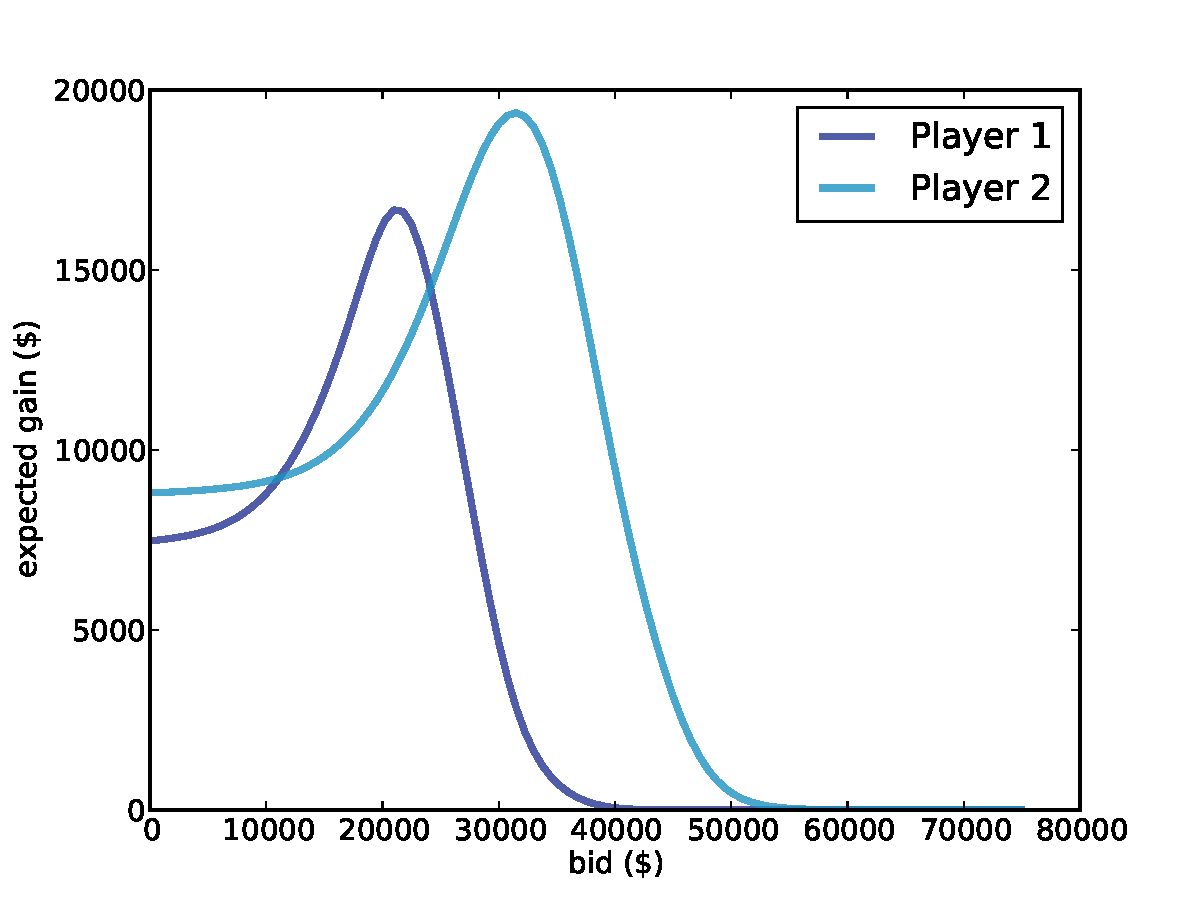
\includegraphics[height=2.5in]{figs/price5.pdf}}
\caption{Expected gain versus bid in a scenario where Player 1's best 
guess is \$20,000 and Player 2's best guess is \$40,000.}
\label{fig.price5}
\end{figure}

{\tt ExpectedGain} invokes {\tt Gain}, which takes a bid and an actual
price and returns the expected gain:

\begin{code}
    def Gain(self, bid, price):
        if bid > price:
            return 0

        diff = price - bid
        prob = self.ProbWin(diff)

        if diff <= 250:
            return 2 * price * prob
        else:
            return price * prob
\end{code}

If you overbid, you get nothing.  Otherwise we compute 
the difference between your bid and the price, which determines
your probability of winning.

If {\tt diff} is less than \$250, you win both showcases.  For
simplicity, I assume that both showcases have the same price.  Since
this outcome is rare, it doesn't make much difference.

Finally, we have to compute the probability of winning based
on {\tt diff}:

\begin{code}
    def ProbWin(self, diff):
        prob = (self.opponent.ProbOverbid() + 
                self.opponent.ProbWorseThan(diff))
        return prob
\end{code}

If your opponent overbids, you win.  Otherwise, you have to hope
that your opponent is off by more than {\tt diff}.  {\tt Player}
provides methods to compute both probabilities:

\begin{code}
# class Player:

    def ProbOverbid(self):
        return self.cdf_diff.Prob(-1)

    def ProbWorseThan(self, diff):
        return 1 - self.cdf_diff.Prob(diff)
\end{code}

This code might be confusing because the computation is now from
the point of view of the opponent, who is computing, ``What is
the probability that I overbid?'' and ``What is the probability
that my bid is off by more than {\tt diff}?''

Both answers are based on the CDF of {\tt diff}.  If the opponent's
{\tt diff} is less than or equal to -1, you win.  If the opponent's
{\tt diff} is worse than yours, you win.  Otherwise you lose.

Finally, here's the code that computes optimal bids:

\begin{code}
# class Player:

    def OptimalBid(self, guess, opponent):
        self.MakeBeliefs(guess)
        calc = GainCalculator(self, opponent)
        bids, gains = calc.ExpectedGains()
        gain, bid = max(zip(gains, bids))
        return bid, gain
\end{code}

Given a guess and an opponent, {\tt OptimalBid} computes
the posterior distribution, instantiates a {\tt GainCalculator},
computes expected gains for a range of bids and returns
the optimal bid and expected gain.  Whew!

Figure~\ref{fig.price5} shows the results for both players,
based on a scenario where Player 1's best guess is \$20,000
and Player 2's best guess is \$40,000.

For Player 1 the optimal bid is \$21,000, yielding an expected
return of almost \$16,700.  This is a case (which turns out
to be unusual) where the optimal bid is actually higher than
the contestant's best guess.

For Player 2 the optimal bid is \$31,500, yielding an expected
return of almost \$19,400.  This is the more typical case where
the optimal bid is less than the best guess.


\section{Discussion}

One of the features of Bayesian estimation is that the
result comes in the form of a posterior distribution.  Classical
estimation usually generates a single point estimate or a confidence
interval, which is sufficient if estimation is the last step in the
process, but if you want to use an estimate as an input to a
subsequent analysis, point estimates and intervals are often not much
help.
\index{distribution}

In this example, we use the posterior distribution
to compute an optimal bid.  The return on a given bid is asymmetric
and discontinuous (if you overbid, you lose), so it would be hard to
solve this problem analytically.  But it is relatively simple to do
computationally.
\index{decision analysis}

Newcomers to Bayesian thinking are often tempted to summarize the
posterior distribution by computing the mean or the maximum
likelihood estimate.  These summaries can be useful, but if that's
all you need, then you probably don't need Bayesian methods in the
first place.
\index{maximum likelihood}
\index{summary statistic}

Bayesian methods are most useful when you can carry the posterior
distribution into the next step of the analysis to perform some
kind of decision analysis, as we did in this chapter, or some kind of
prediction, as we see in the next chapter.




\chapter{Observer Bias}
\label{observer}

\section{The Red Line problem}

In Massachusetts, the Red Line is a subway that connects
Cambridge and Boston.  When I was working in Cambridge I took the Red
Line from Kendall Square to South Station and caught the commuter rail
to Needham.  During rush hour Red Line trains run every 7--8
minutes, on average.
\index{Red Line problem}
\index{Boston}

When I arrived at the station, I could estimate the time until
the next train based on the number of passengers on the platform.
If there were only a few people, I inferred that I just missed
a train and expected to wait about 7 minutes.  If there were
more passengers, I expected the train to arrive sooner.  But if
there were a large number of passengers, I suspected that
trains were not running on schedule, so I would go back to the
street level and get a taxi.

While I was waiting for trains, I thought about how Bayesian
estimation could help predict my wait time and decide when I
should give up and take a taxi.  This chapter presents the
analysis I came up with.

This chapter is based on a project by Brendan Ritter and
Kai Austin, who took a class with me at Olin College.
The code in this chapter is available from
\url{http://thinkbayes.com/redline.py}.  The code I used
to collect data is in \url{http://thinkbayes.com/redline_data.py}.
  For more information
see Section~\ref{download}.
\index{Olin College}


\section{The model}

\begin{figure}
% redline.py
\centerline{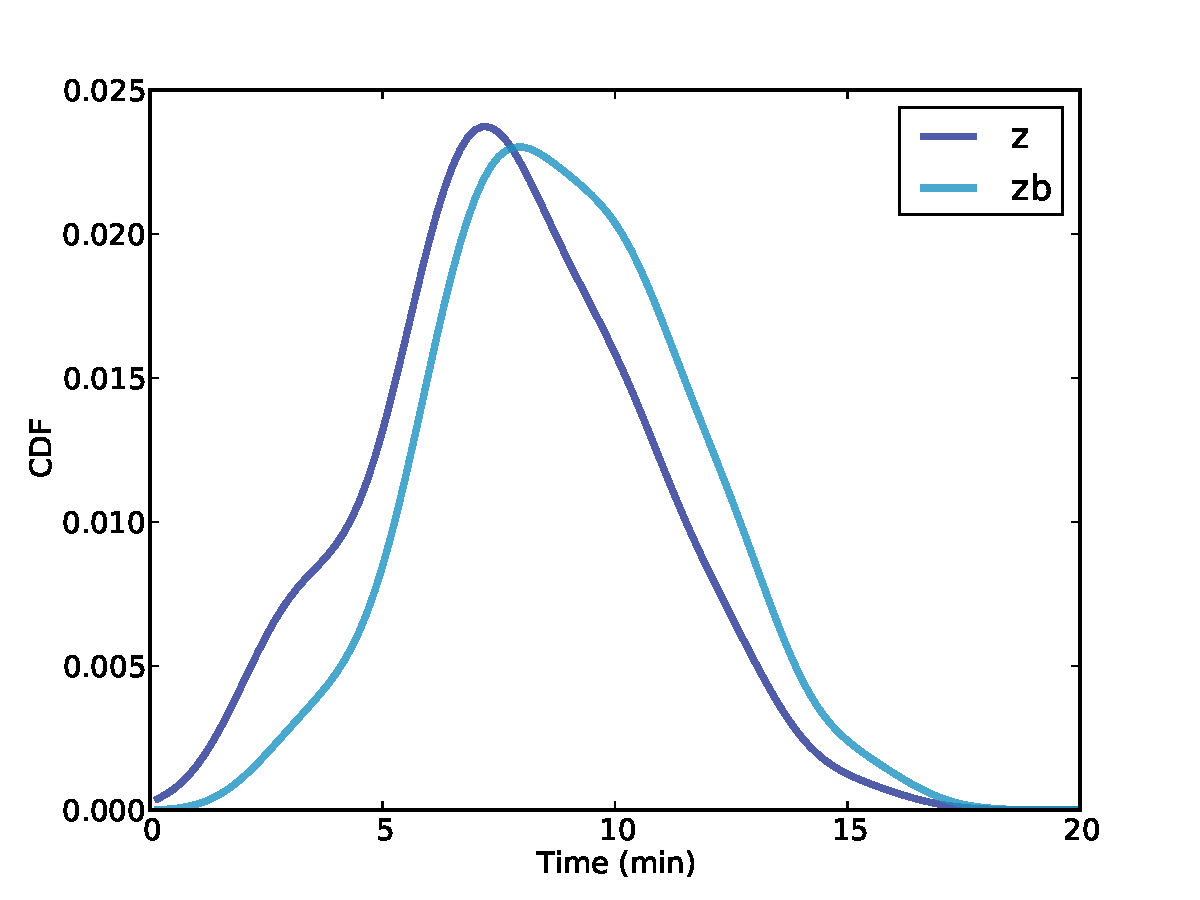
\includegraphics[height=2.5in]{figs/redline0.pdf}}
\caption{PMF of gaps between trains, based on collected data,
smoothed by KDE.  {\tt z} is the actual distribution; {\tt zb}
is the biased distribution seen by passengers. }
\label{fig.redline0}
\end{figure}

Before we get to the analysis, we have to make some
modeling decisions.  First, I will treat passenger arrivals as
a Poisson process, which means I assume that passengers are equally
likely to arrive at any time, and that they arrive at an unknown
rate, $\lambda$, measured in passengers per minute.  Since I
observe passengers during a short period of time, and at the same
time every day, I assume that $\lambda$ is constant.
\index{Poisson process}

On the other hand, the arrival process for trains is not Poisson.
Trains to Boston are supposed to leave from the end of the line
(Alewife station) every 7--8 minutes during peak times, but by the time
they get to Kendall Square, the time between trains varies between 3
and 12 minutes.

To gather data on the time between trains, I wrote a script that
downloads real-time data from
\url{http://www.mbta.com/rider_tools/developers/}, selects south-bound
trains arriving at Kendall square, and records their arrival times
in a database.  I ran the script from 4pm to 6pm every weekday
for 5 days, and recorded about 15 arrivals per day.  Then
I computed the time between consecutive arrivals; the distribution
of these gaps is shown in Figure~\ref{fig.redline0}, labeled {\tt z}.

If you stood on the platform from 4pm to 6pm and recorded the time
between trains, this is the distribution you would see.  But if you
arrive at some random time (without regard to the train schedule) you
would see a different distribution.  The average time
between trains, as seen by a random passenger, is substantially
higher than the true average.

Why?  Because a passenger is more like to arrive during a
large interval than a small one.  Consider a simple example:
suppose that the time between trains is either 5 minutes
or 10 minutes with equal probability.  In that case
the average time between
trains is 7.5 minutes.

But a passenger is more likely to arrive during a 10 minute gap 
than a 5 minute gap; in fact, twice as likely.  If we surveyed
arriving passengers, we would find that 2/3 of them arrived during
a 10 minute gap, and only 1/3 during a 5 minute gap.  So the
average time between trains, as seen by an arriving passenger,
is 8.33 minutes.

This kind of {\bf observer bias} appears in many contexts.  Students
think that classes are bigger than they are because more of them are
in the big classes.  Airline passengers think that planes are fuller
than they are because more of them are on full flights.
\index{observer bias}

In each case, values from the actual distribution are
oversampled in proportion to their value.  In the Red Line example,
a gap that is twice as big is twice as likely to be observed.

So given the actual distribution of gaps, we can compute the
distribution of gaps as seen by passengers.  {\tt BiasPmf}
does this computation:

\begin{code}
def BiasPmf(pmf):
    new_pmf = pmf.Copy()

    for x, p in pmf.Items():
        new_pmf.Mult(x, x)
        
    new_pmf.Normalize()
    return new_pmf
\end{code}

{\tt pmf} is the actual distribution; \verb"new_pmf" is the
biased distribution.  Inside the loop, we multiply the
probability of each value, {\tt x}, by the likelihood it will
be observed, which is proportional to {\tt x}.  Then we
normalize the result.

Figure~\ref{fig.redline0} shows the actual distribution of gaps,
labeled {\tt z}, and the distribution of gaps seen by passengers,
labeled {\tt zb} for ``z biased''.


\section{Wait times}

\begin{figure}
% redline.py
\centerline{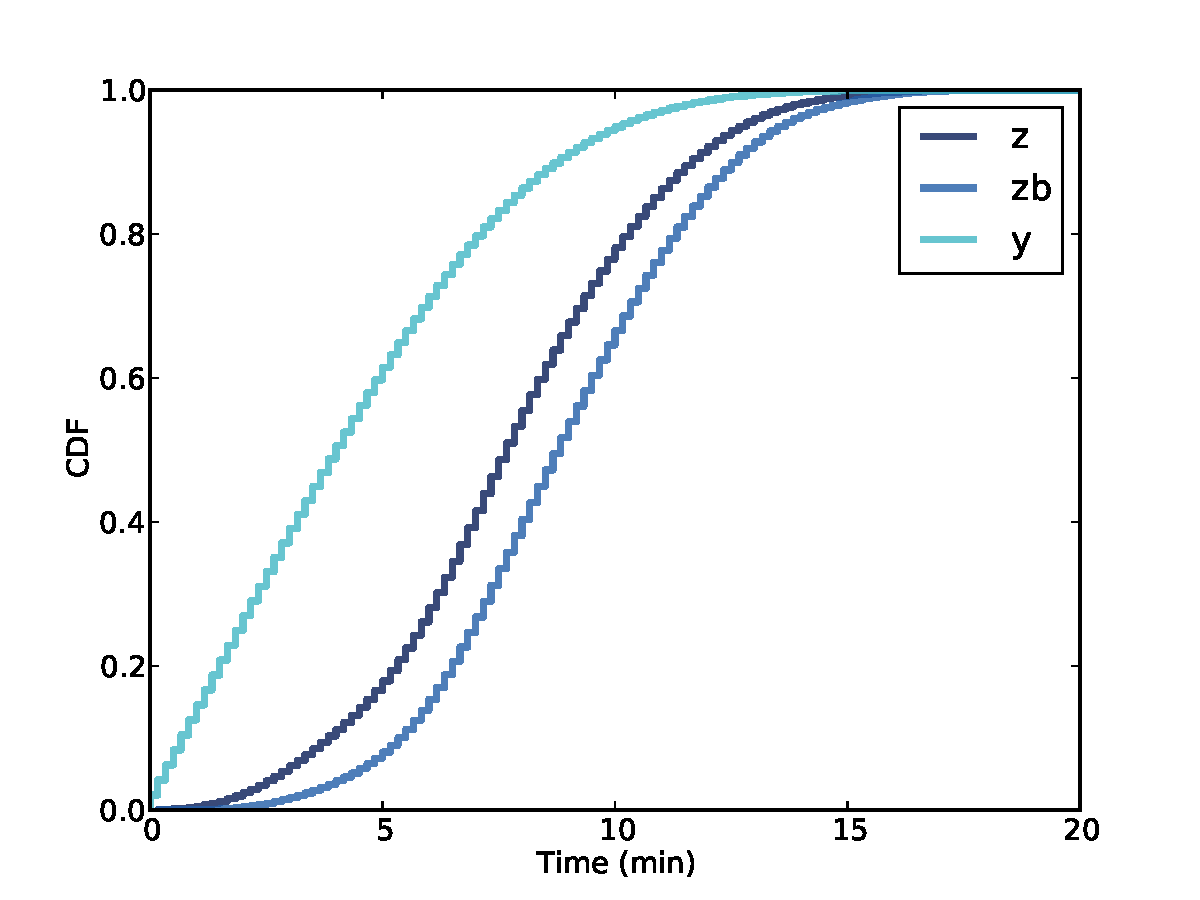
\includegraphics[height=2.5in]{figs/redline2.pdf}}
\caption{CDF of {\tt z}, {\tt zb}, and the wait time seen
by passengers, {\tt y}. }
\label{fig.redline2}
\end{figure}

Wait time, which I call {\tt y}, is the time between the arrival
of a passenger and the next arrival of a train.  Elapsed time, which I
call {\tt x}, is the time between the arrival of the previous
train and the arrival of a passenger.  I chose these definitions
so that {\tt zb = x + y}.

Given the distribution of {\tt zb}, we can compute the distribution of
{\tt y}.  I'll start with a simple case and then generalize.
Suppose, as in the previous example, that {\tt zb} is either 5 minutes
with probability 1/3, or 10 minutes with probability 2/3.

If we arrive at a random time during a 5 minute gap, 
{\tt y} is uniform from 0 to 5 minutes.  If we arrive during a 10
minute gap, {\tt y} is uniform from 0 to 10.  So the overall
distribution is a mixture of uniform distributions weighted
according to the probability of each gap.
\index{uniform distribution}

The following function takes the distribution of {\tt zb} and
computes the distribution of {\tt y}:

\begin{code}
def PmfOfWaitTime(pmf_zb):
    metapmf = thinkbayes.Pmf()
    for gap, prob in pmf_zb.Items():
        uniform = MakeUniformPmf(0, gap)
        metapmf.Set(uniform, prob)

    pmf_y = thinkbayes.MakeMixture(metapmf)
    return pmf_y
\end{code}

{\tt PmfOfWaitTime} makes a meta-Pmf that maps from each uniform
distribution to its probability.  Then it uses {\tt MakeMixture},
which we saw in Section~\ref{mixture}, to compute the mixture.
\index{mixture}
\index{MakeMixture}
\index{meta-Pmf}

{\tt PmfOfWaitTime} also uses {\tt MakeUniformPmf}, defined here:

\begin{code}
def MakeUniformPmf(low, high):
    pmf = thinkbayes.Pmf()
    for x in MakeRange(low=low, high=high):
        pmf.Set(x, 1)
    pmf.Normalize()
    return pmf
\end{code}

{\tt low} and {\tt high} are the range of the uniform distribution,
(both ends included).  Finally, {\tt MakeUniformPmf} uses {\tt
  MakeRange}, defined here:

\begin{code}
def MakeRange(low, high, skip=10):
    return range(low, high+skip, skip)
\end{code}

{\tt MakeRange} defines a set of possible values for wait time
(expressed in seconds).  By default it divides the range into 
10 second intervals.

To encapsulate the process of computing these distributions, I
created a class called {\tt WaitTimeCalculator}:

\begin{code}
class WaitTimeCalculator(object):

    def __init__(self, pmf_z):
        self.pmf_z = pmf_z
        self.pmf_zb = BiasPmf(pmf)

        self.pmf_y = self.PmfOfWaitTime(self.pmf_zb)
        self.pmf_x = self.pmf_y
\end{code}

The parameter, \verb"pmf_z", is the unbiased distribution of {\tt z}.
\verb"pmf_zb" is the biased distribution of gap time, as seen by
passengers.

\verb"pmf_y" is the distribution of wait time.  \verb"pmf_x" is the
distribution of elapsed time, which is the same as the distribution of
wait time.  To see why, remember that for a particular value of
{\tt zp}, the distribution of {\tt y} is uniform from 0 to {\tt zp}.
Also
%
\begin{code}
x = zp - y
\end{code}
%
So the distribution of {\tt x} is also uniform from 0 to {\tt zp}.

Figure~\ref{fig.redline2} shows the distribution of {\tt z}, {\tt zb},
and {\tt y} based on the data I collected from the Red Line web site.

To present these distributions, I am switching from Pmfs to Cdfs.
Most people are more familiar with Pmfs, but I think Cdfs are easier
to interpret, once you get used to them.  And if you want to plot
several distributions on the same axes, Cdfs are the way to go.
\index{Cdf}
\index{cumulative distribution function}

The mean of {\tt z} is 7.8 minutes.  The mean of {\tt zb} is 8.8
minutes, about 13\% higher.  The mean of {\tt y} is 4.4, half
the mean of {\tt zb}.

As an aside, the Red Line schedule reports that trains run every
9 minutes during peak times.  This is close to the average of
{\tt zb}, but higher than the average of {\tt z}.  I exchanged email
with a representative of the MBTA, who confirmed that the reported
time between trains is deliberately conservative in order to
account for variability.


\section{Predicting wait times}
\label{elapsed}

\begin{figure}
% redline.py
\centerline{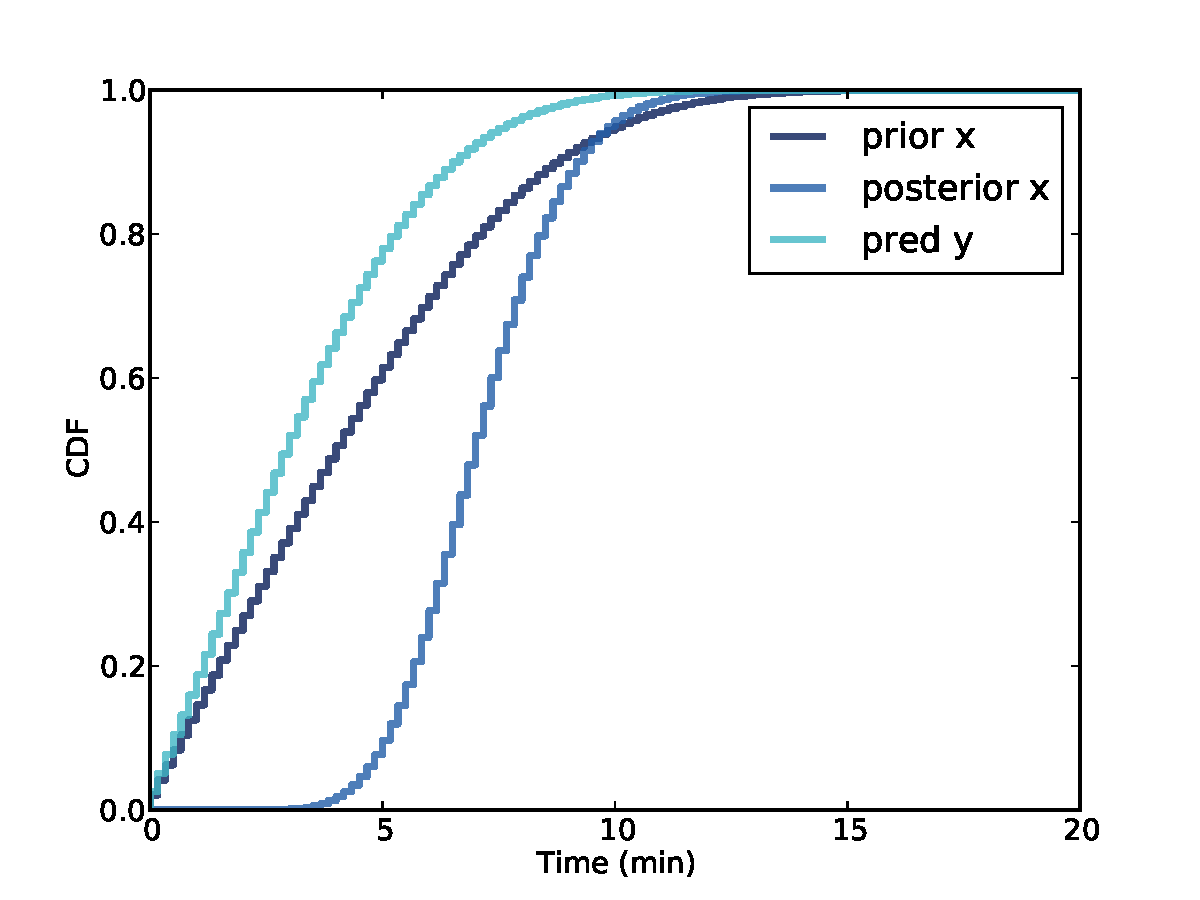
\includegraphics[height=2.5in]{figs/redline3.pdf}}
\caption{Prior and posterior of {\tt x} and predicted {\tt y}. }
\label{fig.redline3}
\end{figure}

Let's get back to the motivating question: suppose that when
I arrive at the platform I see 10 people waiting.
How long should I expect to wait until the next train arrives?

As always, let's start with the easiest version of the problem
and work our way up.  Suppose we are given the actual distribution of
{\tt z}, and we know that the passenger arrival rate,
$\lambda$, is 2 passengers per minute.

In that case we can:

\begin{enumerate}

\item Use the distribution of {\tt z} to compute
the prior distribution of {\tt zp}, the time between trains
as seen by a passenger.

\item Then we can use the number of passengers to estimate the distribution
of {\tt x}, the elapsed time since the last train.

\item Finally, we use the relation {\tt y = zp - x} to get the
distribution of {\tt y}.

\end{enumerate}

The first step is to create a {\tt WaitTimeCalculator} that
encapsulates the distributions of {\tt zp}, {\tt x},
and {\tt y}, prior to taking into account the number of
passengers.

\begin{code}
    wtc = WaitTimeCalculator(pmf_z)
\end{code}

\verb"pmf_z" is the given distribution of gap times.

The next step is to make an {\tt ElapsedTimeEstimator} (defined
below), which encapsulates the posterior distribution of {\tt x} and
the predictive distribution of {\tt y}.
\index{predictive distribution}

\begin{code}
    ete = ElapsedTimeEstimator(wtc,
                               lam=2.0/60,
                               num_passengers=15)
\end{code}

The parameters are the {\tt WaitTimeCalculator}, the passenger
arrival rate, {\tt lam} (expressed in passengers per second),
and the observed number of passengers, let's say 15.

Here is the definition of {\tt ElapsedTimeEstimator}:

\begin{code}
class ElapsedTimeEstimator(object):

    def __init__(self, wtc, lam, num_passengers):
        self.prior_x = Elapsed(wtc.pmf_x)

        self.post_x = self.prior_x.Copy()
        self.post_x.Update((lam, num_passengers))

        self.pmf_y = PredictWaitTime(wtc.pmf_zb, self.post_x)
\end{code}

\verb"prior_x" and \verb"posterior_x" are the prior and
posterior distributions of elapsed time.  \verb"pmf_y" is
the predictive distribution of wait time.

{\tt ElapsedTimeEstimator} uses {\tt Elapsed} and {\tt PredictWaitTime},
defined below.

{\tt Elapsed} is a Suite that represents the hypothetical
distribution of {\tt x}.  The prior distribution of {\tt x}
comes straight from the {\tt WaitTimeCalculator}.  Then we
use the data, which consists of the arrival rate, {\tt lam},
and the number of passengers on the platform, to compute
the posterior distribution.

Here's the definition of {\tt Elapsed}:

\begin{code}
class Elapsed(thinkbayes.Suite):

    def Likelihood(self, data, hypo):
        x = hypo
        lam, k = data
        like = thinkbayes.EvalPoissonPmf(k, lam * x)
        return like
\end{code}

As always, {\tt Likelihood} takes a hypothesis and data, and
computes the likelihood of the data under the hypothesis.
In this case {\tt hypo} is the elapsed time since the last train
and {\tt data} is a tuple of {\tt lam} and the number of
passengers.
\index{likelihood}

The likelihood of the data is the probability of getting
{\tt k} arrivals in {\tt x} time, given arrival rate
{\tt lam}.  We compute that using the PMF of the Poisson
distribution.
\index{Poisson distribution}

Finally, here's the definition of {\tt PredictWaitTime}:

\begin{code}
def PredictWaitTime(pmf_zb, pmf_x):
    pmf_y = pmf_zb - pmf_x
    RemoveNegatives(pmf_y)
    return pmf_y
\end{code}

\verb"pmf_zb" is the distribution of gaps between trains;
\verb"pmf_x" is the distribution of elapsed time, based on
the observed number of passengers.  Since {\tt y = zb - x},
we can compute

\begin{code}
    pmf_y = pmf_zb - pmf_x
\end{code}

The subtraction operator invokes \verb"Pmf.__sub__", which enumerates
all pairs of {\tt zb} and {\tt x}, computes the differences, and adds
the results to \verb"pmf_y".

The resulting Pmf includes some negative values, which we know are
impossible.  For example, if you arrive during a gap of 5 minutes, you
can't wait more than 5 minutes.  {\tt RemoveNegatives} removes the
impossible values from the distribution and renormalizes.

\begin{code}
def RemoveNegatives(pmf):
    for val in pmf.Values():
        if val < 0:
            pmf.Remove(val)
    pmf.Normalize()
\end{code}

Figure~\ref{fig.redline3} shows the results.  The prior distribution
of {\tt x} is the same as the distribution of {\tt y} in
Figure~\ref{fig.redline2}.  The posterior distribution of {\tt x}
shows that, after seeing 15 passengers on the platform, we believe
that the time since the last train is probably 5-10 minutes.  The
predictive distribution of {\tt y} indicates that we expect the next
train in less than 5 minutes, with about 80\% confidence.
\index{predictive distribution}


\section{Estimating the arrival rate}

\begin{figure}
% redline.py
\centerline{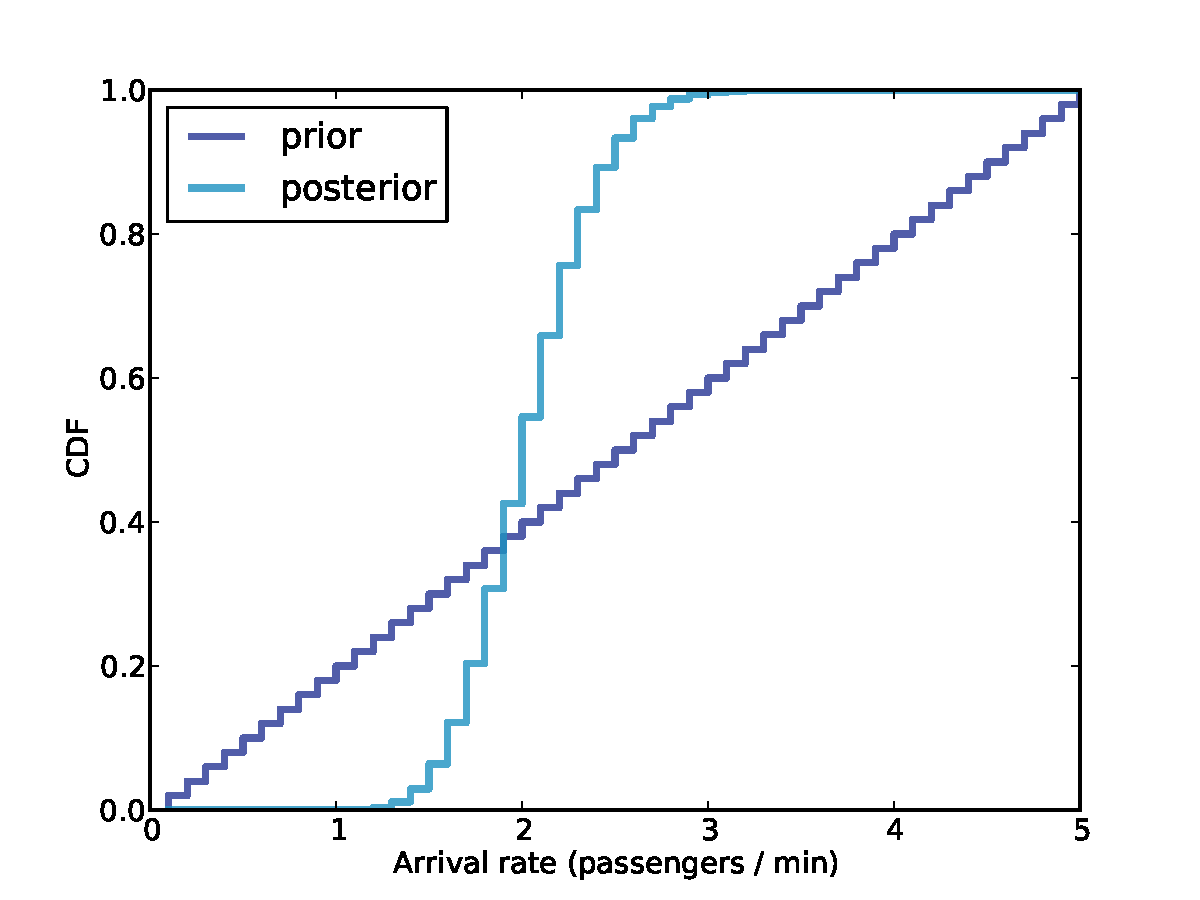
\includegraphics[height=2.5in]{figs/redline1.pdf}}
\caption{Prior and posterior distributions of {\tt lam} based
on five days of passenger data. }
\label{fig.redline1}
\end{figure}

The analysis so far has been based on the assumption that we know (1)
the distribution of gaps and (2) the passenger arrival rate.  Now we
are ready to relax the second assumption.

Suppose that you just moved to Boston, so you don't know much about
the passenger arrival rate on the Red Line.  After a few days of
commuting, you could make a guess, at least qualitatively.  With
a little more effort, you could estimate $\lambda$ quantitatively.
\index{arrival rate}

Each day when you arrive at the platform, you should note the
time and the number of passengers waiting (if the platform is too
big, you could choose a sample area).  Then you should record your
wait time and the
number of new arrivals while you are waiting.

After five days, you might have data like this:
%
\begin{code}
k1      y     k2
--     ---    --
17     4.6     9
22     1.0     0
23     1.4     4
18     5.4    12
4      5.8    11
\end{code}
%
where {\tt k1} is the number of passengers waiting when you arrive,
{\tt y} is your wait time in minutes, and {\tt k2} is the number of
passengers who arrive while you are waiting.

Over the course of one week, you waited 18 minutes and saw 36
passengers arrive, so you would estimate that the arrival rate is
2 passengers per minute.  For practical purposes that estimate is
good enough, but for the sake of completeness I
will compute a posterior distribution for $\lambda$ and show how
to use that distribution in the rest of the analysis.

{\tt ArrivalRate} is a {\tt Suite} that represents hypotheses about
$\lambda$.  As always, {\tt Likelihood} takes a hypothesis and data,
and computes the likelihood of the data under the hypothesis.

In this case the hypothesis is a value of $\lambda$.  The data is a
pair, {\tt y, k}, where {\tt y} is a wait time and {\tt k} is the
number of passengers that arrived.

\begin{code}
class ArrivalRate(thinkbayes.Suite):

    def Likelihood(self, data, hypo):
        lam = hypo
        y, k = data
        like = thinkbayes.EvalPoissonPmf(k, lam * y)
        return like
\end{code}

This {\tt Likelihood} might look familiar; it
is almost identical to {\tt Elapsed.Likelihood} in
Section~\ref{elapsed}.  The difference is that in {\tt
  Elapsed.Likelihood} the hypothesis is {\tt x}, the elapsed time; in
{\tt ArrivalRate.Likelihood} the hypothesis is {\tt lam}, the arrival
rate.  But in both cases the likelihood is the probability of seeing
{\tt k} arrivals in some period of time, given {\tt lam}.

{\tt ArrivalRateEstimator} encapsulates the process of estimating
$\lambda$.  The parameter, \verb"passenger_data", is a list
of {\tt k1, y, k2} tuples, as in the table above.
\index{numpy}

\begin{code}
class ArrivalRateEstimator(object):

    def __init__(self, passenger_data):
        low, high = 0, 5
        n = 51
        hypos = numpy.linspace(low, high, n) / 60

        self.prior_lam = ArrivalRate(hypos)

        self.post_lam = self.prior_lam.Copy()
        for k1, y, k2 in passenger_data:
            self.post_lam.Update((y, k2))
\end{code}

\verb"__init__" builds
{\tt hypos}, which is a sequence of hypothetical values for {\tt lam},
then builds the prior distribution, \verb"prior_lam".
The {\tt for} loop updates the prior with data, yielding the posterior
distribution, \verb"post_lam".

Figure~\ref{fig.redline1} shows
the prior and posterior distributions.  As expected, the mean and
median of the posterior are near the observed rate, 2 passengers per
minute.  But the spread of the posterior distribution captures our
uncertainty about $\lambda$ based on a small sample.


\section{Incorporating uncertainty}

\begin{figure}
% redline.py
\centerline{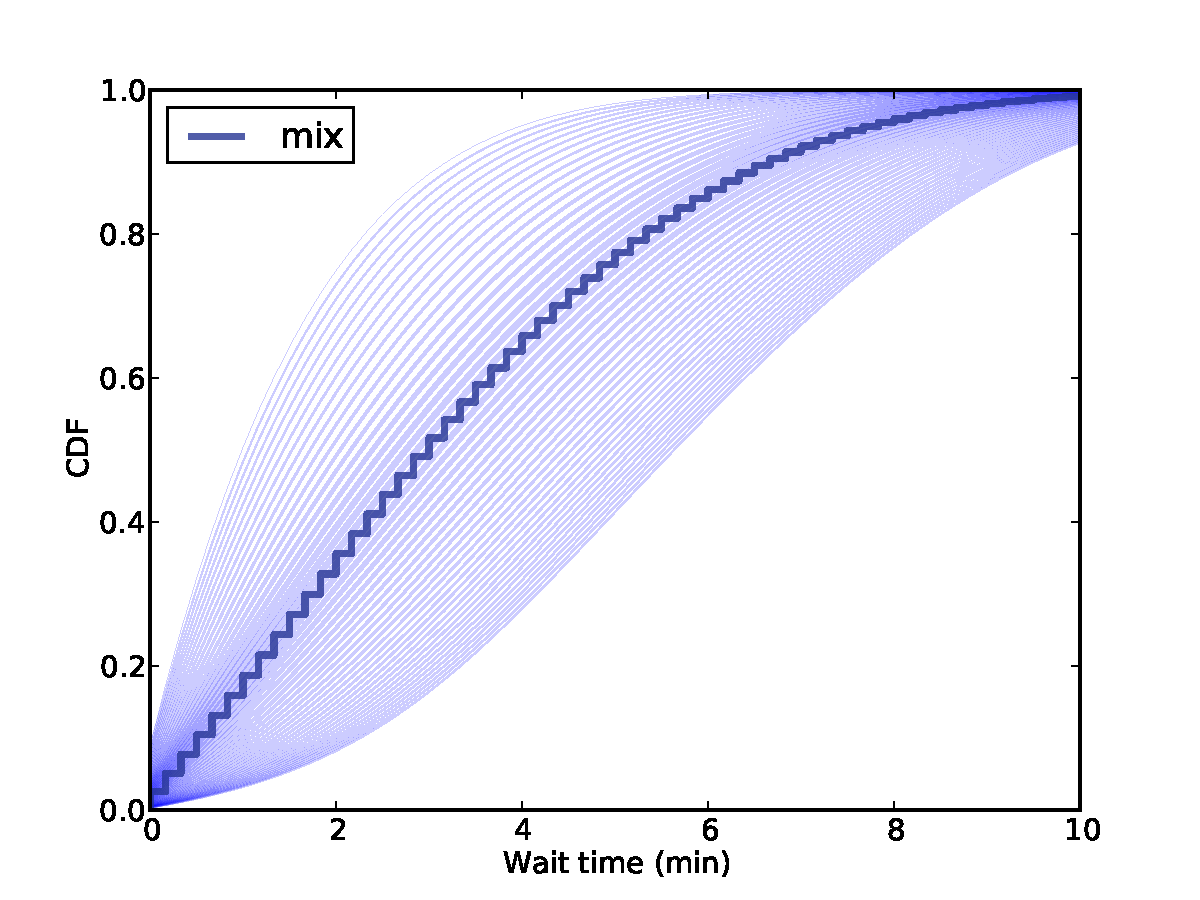
\includegraphics[height=2.5in]{figs/redline4.pdf}}
\caption{Predictive distributions of {\tt y} for possible values
  of {\tt lam}. }
\label{fig.redline4}
\end{figure}

Whenever there is uncertainty about one of the inputs to an analysis,
we can take it into account by a process like this:
\index{uncertainty}

\begin{enumerate}

\item Implement the analysis based on a deterministic value of the
  uncertain parameter (in this case $\lambda$).

\item Compute the distribution of the uncertain parameter.

\item Run the analysis for each value of the parameter, and generate a
  set of predictive distributions.
\index{predictive distribution}

\item Compute a mixture of the predictive distributions, using the
  weights from the distribution of the parameter.
\index{mixture}

\end{enumerate}

We have already done steps (1) and (2).  I wrote a class
called {\tt WaitMixtureEstimator} to handle steps (3) and (4).

\begin{code}
class WaitMixtureEstimator(object):

    def __init__(self, wtc, are, num_passengers=15):
        self.metapmf = thinkbayes.Pmf()

        for lam, prob in sorted(are.post_lam.Items()):
            ete = ElapsedTimeEstimator(wtc, lam, num_passengers)
            self.metapmf.Set(ete.pmf_y, prob)

        self.mixture = thinkbayes.MakeMixture(self.metapmf)
\end{code}

{\tt wtc} is the {\tt WaitTimeCalculator} that contains the
distribution of {\tt zb}.  {\tt are} is the {\tt ArrivalTimeEstimator}
that contains the distribution of {\tt lam}.

The first line makes a meta-Pmf that maps from each possible
distribution of {\tt y} to its probability.  For each value
of {\tt lam}, we use {\tt ElapsedTimeEstimator} to
compute the corresponding distribution of
{\tt y} and store it in the Meta-Pmf.  Then
we use {\tt MakeMixture} to compute the mixture.
\index{MakeMixture}
\index{meta-Pmf}
\index{mixture}

%For purposes of comparison, I also compute the distribution of
%{\tt y} based on a single point estimate of {\tt lam}, which is
%the mean of the posterior distribution.

Figure~\ref{fig.redline4} shows the results.  The shaded lines
in the background are the distributions of {\tt y} for each value
of {\tt lam}, with line thickness that represents likelihood.
The dark line is the mixture of these distributions.

In this case we could get a very similar result using a single point
estimate of {\tt lam}.  So it was not necessary, for practical purposes,
to include the uncertainty of the estimate.

In general, it is important to include variability if the system
response is non-linear; that is, if small changes in the input can
cause big changes in the output.  In this case, posterior variability
in {\tt lam} is small and the system response is approximately
linear for small perturbations.
\index{non-linear}


\section{Decision analysis}

\begin{figure}
% redline.py
\centerline{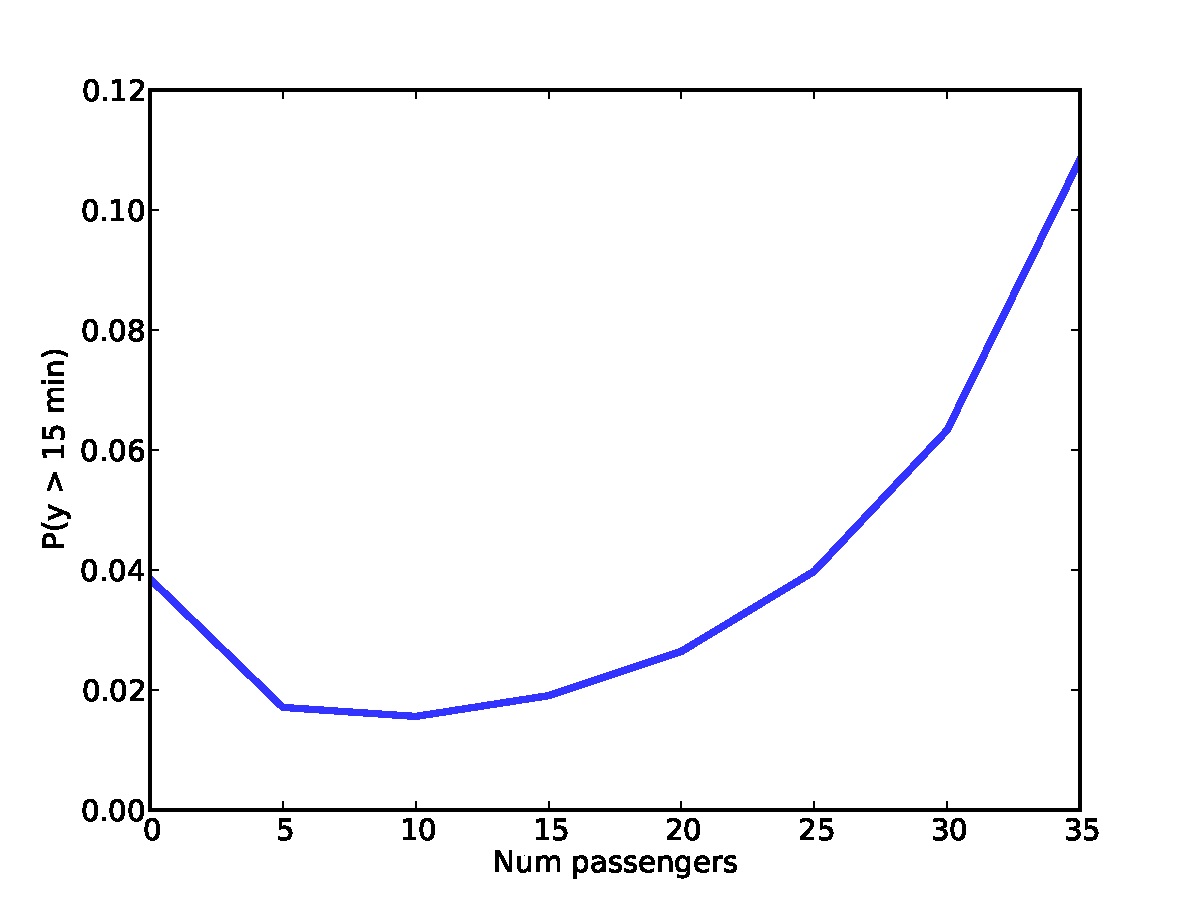
\includegraphics[height=2.5in]{figs/redline5.pdf}}
\caption{Probability that wait time exceeds 15 minutes as
a function of the number of passengers on the platform. }
\label{fig.redline5}
\end{figure}

At this point we can use the number of passengers on the platform
to predict the distribution of wait times.  Now
let's get to the second part of the question: when should I stop
waiting for the train and go catch a taxi?
\index{decision analysis}

Remember that in the original scenario, I am trying to get to
South Station to catch the commuter rail.  Suppose I leave
the office with enough time that I can wait 15 minutes
and still make my connection at South Station.

In that case I would like to know the probability that {\tt y} exceeds
15 minutes as a function of \verb"num_passengers".  It is easy enough
to use the
analysis from Section~\ref{elapsed} and run it for a range of
\verb"num_passengers".

But there's a problem.
The analysis is sensitive to the frequency of long delays, and
because long delays are rare, it is hard to estimate
their frequency.

I only have data from one week,
and the longest delay I observed was 15 minutes.  So I can't
estimate the frequency of longer delays accurately.

However, I can use previous observations to make at least a coarse
estimate.  When I commuted by Red Line for a year, I saw three long
delays caused by a signaling problem, a power outage, and ``police
activity'' at another stop.  So I estimate that there are about
3 major delays per year.

But remember that my observations are biased.  I am more likely
to observe long delays because they affect a large number
of passengers.  So we should treat my observations as a sample
of {\tt zb} rather than {\tt z}.  Here's how we can do that.
\index{observer bias}

During my year of commuting, I took the Red Line home about 220
times.  So I take the observed gap times, \verb"gap_times",
generate a sample of 220 gaps, and compute their Pmf:

\begin{code}
    n = 220
    cdf_z = thinkbayes.MakeCdfFromList(gap_times)
    sample_z = cdf_z.Sample(n)
    pmf_z = thinkbayes.MakePmfFromList(sample_z)
\end{code}

Next I bias \verb"pmf_z" to get the distribution of
{\tt zb}, draw a sample, and then add in delays of
30, 40, and 50 minutes (expressed in seconds):

\begin{code}
    cdf_zp = BiasPmf(pmf_z).MakeCdf()
    sample_zb = cdf_zp.Sample(n) + [1800, 2400, 3000]
\end{code}

{\tt Cdf.Sample} is more efficient than {\tt Pmf.Sample}, so it
is usually faster to convert a Pmf to a Cdf before sampling.

Next I use the sample of {\tt zb} to estimate a Pdf using
KDE, and then convert the Pdf to a Pmf:

\begin{code}
    pdf_zb = thinkbayes.EstimatedPdf(sample_zb)
    xs = MakeRange(low=60)
    pmf_zb = pdf_zb.MakePmf(xs)
\end{code}

Finally I unbias the distribution of {\tt zb} to get the
distribution of {\tt z}, which I use to create the
{\tt WaitTimeCalculator}:

\begin{code}
    pmf_z = UnbiasPmf(pmf_zb)
    wtc = WaitTimeCalculator(pmf_z)
\end{code}

This process is complicated, but
all of the steps are operations we have seen before.
Now we are ready to compute the probability of a long wait.

\begin{code}
def ProbLongWait(num_passengers, minutes):
    ete = ElapsedTimeEstimator(wtc, lam, num_passengers)
    cdf_y = ete.pmf_y.MakeCdf()
    prob = 1 - cdf_y.Prob(minutes * 60)
\end{code}

Given the number of passengers on the platform,
{\tt ProbLongWait} 
makes an {\tt ElapsedTimeEstimator},
extracts the distribution of wait time, and 
computes 
the probability that wait time
exceeds {\tt minutes}.

Figure~\ref{fig.redline5} shows the result.  When the number of
passengers is less than 20, we infer that the system is
operating normally, so the probability of a long delay is small.
If there are 30 passengers, we estimate that it has been 15
minutes since the last train; that's longer than a normal delay,
so we infer that something is wrong and expect longer delays.

If we are willing to accept a 10\% chance of missing the connection
at South Station, we should stay and wait as long as there
are fewer than 30 passengers, and take a taxi if there are more.

Or, to take this analysis one step further, we could quantify the cost
of missing the connection and the cost of taking a taxi, then choose
the threshold that minimizes expected cost.

\section{Discussion}

The analysis so far has been based on the assumption that the
arrival rate of passengers is the same every day.  For a commuter
train during rush hour, that might not be a bad assumption, but
there are some obvious exceptions.  For example, if there is a special
event nearby, a large number of people might arrive at the same time.
In that case, the estimate of {\tt lam} would be too low, so the
estimates of {\tt x} and {\tt y} would be too high.

If special events are as common as major delays, it would
be important to include them in the model.  We could do that by
extending the distribution of {\tt lam} to include occasional
large values.

We started with the assumption that we know
distribution of {\tt z}.
As an alternative, a passenger could estimate {\tt z}, but it would
not be easy.
As a passenger, you only
observe only your own wait time, {\tt y}.  Unless you skip
the first train and wait for the second, you don't
observe the gap between trains, {\tt z}.

However, we could make some inferences about {\tt zb}.  If we note
the number of passengers waiting when we arrive, we can estimate
the elapsed time since the last train, {\tt x}.  Then we observe
{\tt y}.  If we add the posterior distribution of {\tt x} to
the observed {\tt y}, we get a distribution that represents
our posterior belief about the observed value of {\tt zb}.

We can use this distribution to update our beliefs about the
distribution of {\tt zb}.  Finally, we can compute the
inverse of {\tt BiasPmf} to get from the distribution of {\tt zb}
to the distribution of {\tt z}.

I leave this analysis as an exercise for the
reader.  One suggestion: you should read Chapter~\ref{species} first.
You can find the outline of
a solution in \url{http://thinkbayes.com/redline.py}.
  For more information
see Section~\ref{download}.

\section{Exercises}

\begin{exercise}
This exercise is from
MacKay, {\em Information Theory, Inference, and Learning Algorithms}:
\index{MacKay, David}

\begin{quote}
    Unstable particles are emitted from a source and decay at a
distance $x$, a real number that has an exponential probability
distribution with [parameter] $\lambda$.  Decay events can only be
observed if they occur in a window extending from $x=1$ cm to $x=20$
cm.  $N$ decays are observed at locations $\{ 1.5, 2, 3, 4, 5, 12 \}$
cm.  What is the posterior distribution of $\lambda$?

\end{quote}

You can download a solution to this exercise from
\url{http://thinkbayes.com/decay.py}.

\end{exercise}


\chapter{Two Dimensions}
\label{paintball}

\section{Paintball}

Paintball is a sport in which competing teams try to shoot each other
with guns that fire paint-filled pellets that break on impact, leaving
a colorful mark on the target.  It is usually played in an
arena decorated with barriers and other objects that can be
used as cover.
\index{Paintball problem}

Suppose you are playing paintball in an indoor arena 30 feet
wide and 50 feet long.  You are standing near one of the 30 foot
walls, and you suspect that one of your opponents has taken cover
nearby.  Along the wall, you see several paint spatters, all the same
color, that you think your opponent fired recently.

The spatters are at 15, 16, 18, and 21 feet, measured from the
lower-left corner of the room.  Based on these data, where do you
think your opponent is hiding?

Figure~\ref{fig.paintball} shows a diagram of the arena.  Using the
lower-left corner of the room as the origin, I denote the unknown
location of the shooter with coordinates $\alpha$ and $\beta$, or {\tt
  alpha} and {\tt beta}.  The location of a spatter is labeled
{\tt x}.  The angle the opponent shoots at is $\theta$ or {\tt theta}.

The Paintball problem is a modified version
of the Lighthouse problem, a common example of Bayesian analysis.  My
notation follows the presentation of the problem in D.S.~Sivia's, {\it Data
  Analysis: a Bayesian Tutorial, Second Edition} (Oxford, 2006).
\index{Sivia, D.S.}

You can download the code in this chapter from
\url{http://thinkbayes.com/paintball.py}.  For more information see
Section~\ref{download}.


\section{The suite}

\begin{figure}
% paintball.py
\centerline{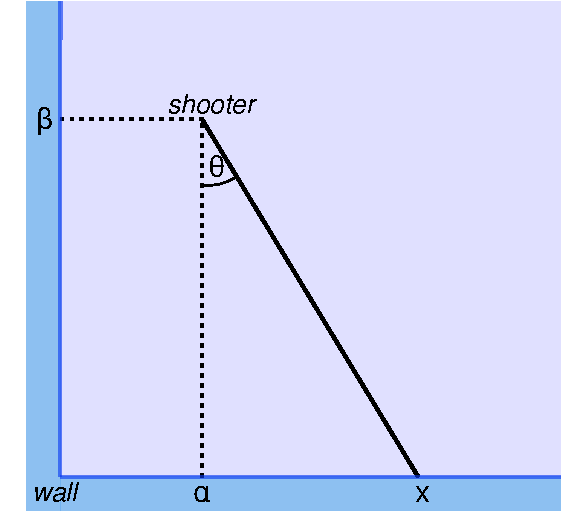
\includegraphics[height=2.5in]{figs/paintball.pdf}}
\caption{Diagram of the layout for the paintball problem.}
\label{fig.paintball}
\end{figure}

To get started, we need a Suite that represents a set of hypotheses
about the location of the opponent.  Each hypothesis is a
pair of coordinates: {\tt (alpha, beta)}.

Here is the definition of the Paintball suite:

\begin{code}
class Paintball(thinkbayes.Suite, thinkbayes.Joint):

    def __init__(self, alphas, betas, locations):
        self.locations = locations
        pairs = [(alpha, beta) 
                 for alpha in alphas 
                 for beta in betas]
        thinkbayes.Suite.__init__(self, pairs)
\end{code}

{\tt Paintball} inherits from {\tt Suite}, which we have seen before,
and {\tt Joint}, which I will explain soon.
\index{Joint pmf}

{\tt alphas} is the list of possible values for {\tt alpha}; {\tt
  betas} is the list of values for {\tt beta}.  {\tt pairs} is a list
of all {\tt (alpha, beta)} pairs.

{\tt locations} is a list of possible locations along
the wall; it is stored for use in {\tt Likelihood}.

\begin{figure}
% paintball.py
\centerline{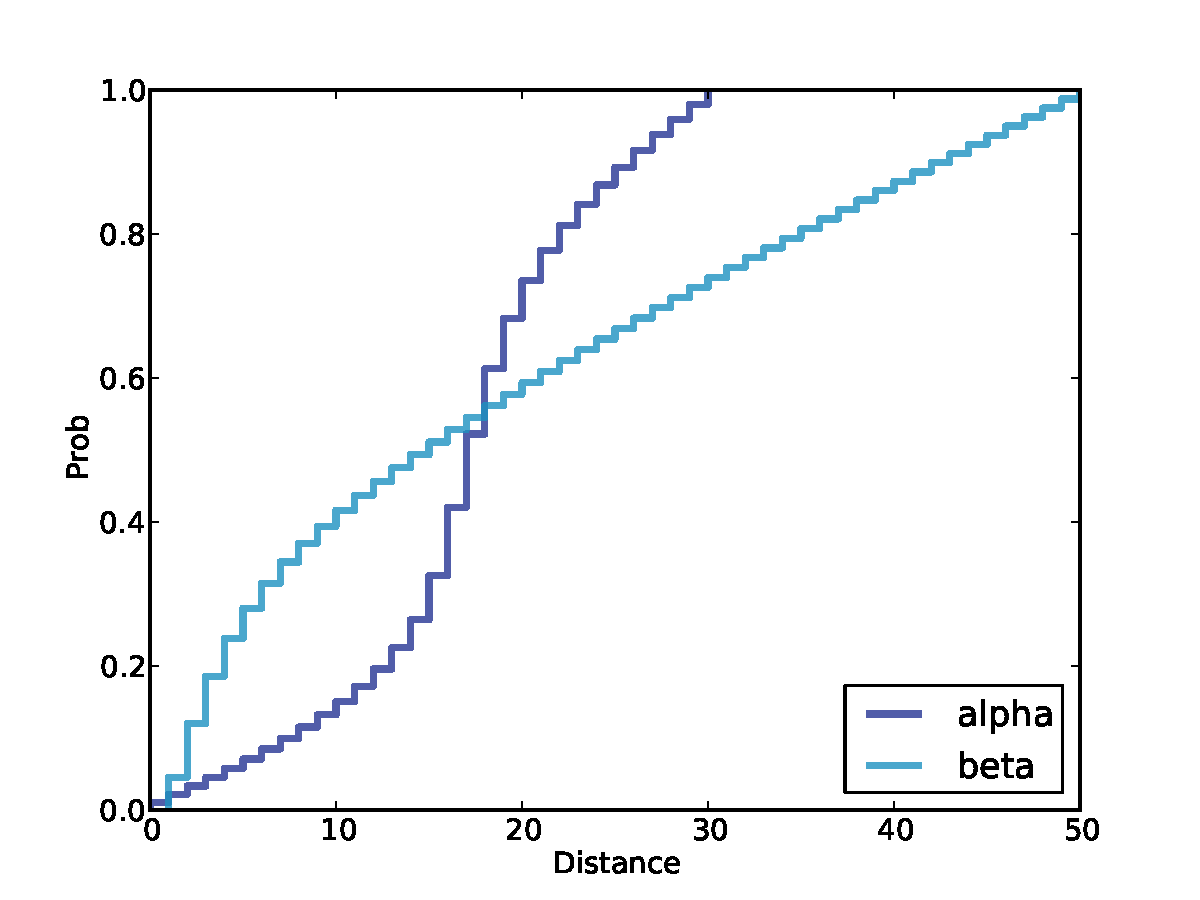
\includegraphics[height=2.5in]{figs/paintball2.pdf}}
\caption{Posterior CDFs for {\tt alpha} and {\tt beta}, given the data.}
\label{fig.paintball2}
\end{figure}

The room is 30 feet wide and 50 feet long, so here's the code that
creates the suite:

\begin{code}
    alphas = range(0, 31)
    betas = range(1, 51)
    locations = range(0, 31)

    suite = Paintball(alphas, betas, locations)
\end{code}

This prior distribution assumes that all locations in the room are
equally likely.  Given a map of the room, we might choose a more
detailed prior, but we'll start simple.


\section{Trigonometry}

Now we need a likelihood function, which means we have to figure
out the likelihood of hitting any spot along the wall, given
the location of the opponent.
\index{likelihood}

As a simple model, imagine that the opponent is like a rotating
turret, equally likely to shoot in any direction.
In that case, he is most likely to hit
the wall at location {\tt alpha}, and less likely to hit the wall far
away from {\tt alpha}.
\index{trigonometry}

With a little trigonometry, we can compute the probability of hitting
any spot along the wall.  Imagine that the shooter fires a shot at
angle $\theta$; the pellet would hit the wall at location $x$, where
%
\[ x - \alpha = \beta \tan \theta \]
%
Solving this equation for $\theta$ yields
%
\[ \theta = tan^{-1} \left( \frac{x - \alpha}{\beta} \right) \]
%
So given a location on the wall, we can find $\theta$.

Taking the derivative of the first equation with respect to
$\theta$ yields
%
\[ \frac{dx}{d\theta} = \frac{\beta}{\cos^2 \theta} \]
%
This derivative is what I'll call the ``strafing speed'',
which is the speed of the target location along the wall as $\theta$
increases.  The probability of hitting a given point on the wall is
inversely related to strafing speed.
\index{strafing speed}

If we know the coordinates of the shooter and a location 
along the wall, we can compute strafing speed:

\begin{code}
def StrafingSpeed(alpha, beta, x):
    theta = math.atan2(x - alpha, beta)
    speed = beta / math.cos(theta)**2
    return speed
\end{code}

{\tt alpha} and {\tt beta} are the coordinates of the shooter;
{\tt x} is the location of a spatter.  The result is
the derivative of {\tt x} with respect to {\tt theta}.

\begin{figure}
% paintball.py
\centerline{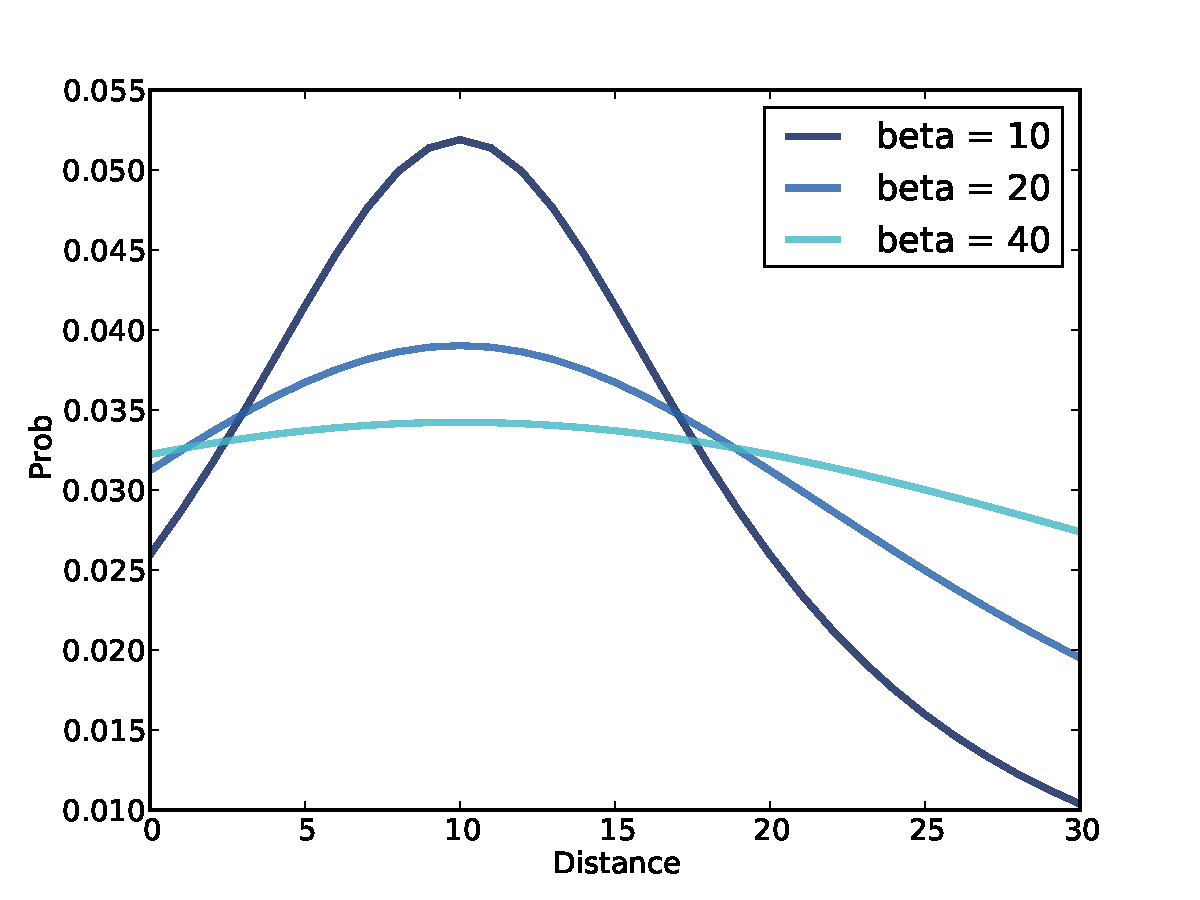
\includegraphics[height=2.5in]{figs/paintball1.pdf}}
\caption{PMF of location given {\tt alpha=10}, for several values of
  {\tt beta}.}
\label{fig.paintball1}
\end{figure}

Now we can compute a Pmf that represents the probability of hitting
any location on the wall.  {\tt MakeLocationPmf} takes {\tt alpha} and
{\tt beta}, the coordinates of the shooter, and {\tt locations}, a
list of possible values of {\tt x}.

\begin{code}
def MakeLocationPmf(alpha, beta, locations):
    pmf = thinkbayes.Pmf()
    for x in locations:
        prob = 1.0 / StrafingSpeed(alpha, beta, x)
        pmf.Set(x, prob)
    pmf.Normalize()
    return pmf
\end{code}

{\tt MakeLocationPmf} computes the probability of hitting
each location, which is inversely related to
strafing speed.  The result is a Pmf of locations and their
probabilities.

Figure~\ref{fig.paintball1} shows the Pmf of location with {\tt alpha
  = 10} and a range of values for {\tt beta}.  For all values of beta
the most likely spatter location is {\tt x = 10}; as {\tt beta}
increases, so does the spread of the Pmf.



\section{Likelihood}

Now all we need is a likelihood function.
We can use {\tt MakeLocationPmf} to compute the likelihood
of any value of {\tt x}, given the coordinates of the opponent.
\index{likelihood}

\begin{code}
    def Likelihood(self, data, hypo):
        alpha, beta = hypo
        x = data
        pmf = MakeLocationPmf(alpha, beta, self.locations)
        like = pmf.Prob(x)
        return like
\end{code}

Again, {\tt alpha} and {\tt beta} are the hypothetical coordinates of
the shooter, and {\tt x} is the location of an observed spatter.

{\tt pmf} contains the probability of each location, given the
coordinates of the shooter.  From this Pmf, we select the probability
of the observed location.

And we're done.  To update the suite, we can use {\tt UpdateSet},
which is inherited from {\tt Suite}.

\begin{code}
suite.UpdateSet([15, 16, 18, 21])
\end{code}

The result is a distribution that maps each {\tt (alpha, beta)} pair
to a posterior probability.


\section{Joint distributions}

When each value in a distribution is a tuple of variables, it is
called a {\bf joint distribution} because it represents the
distributions of the variables together, that is ``jointly''.
A joint distribution contains the distributions of the variables,
as well as information about the relationships among them.
\index{joint distribution}

Given a joint distribution, we can compute the distributions
of each variable independently, which are called the {\bf marginal
distributions}.
\index{marginal distribution}
\index{Joint}

{\tt thinkbayes.Joint} provides a method that computes marginal
distributions:

\begin{code}
# class Joint:

    def Marginal(self, i):
        pmf = Pmf()
        for vs, prob in self.Items():
            pmf.Incr(vs[i], prob)
        return pmf
\end{code}

{\tt i} is the index of the variable we want; in this example
{\tt i=0} indicates the distribution of {\tt alpha}, and
{\tt i=1} indicates the distribution of {\tt beta}.

Here's the code that extracts the marginal distributions:

\begin{code}
    marginal_alpha = suite.Marginal(0)
    marginal_beta = suite.Marginal(1)
\end{code}

Figure~\ref{fig.paintball2} shows the results (converted to CDFs).
The median value for {\tt alpha} is 18, near the center of mass of
the observed spatters.  For {\tt beta}, the most likely values are
close to the wall, but beyond 10 feet the distribution is almost
uniform, which indicates that the data do not distinguish strongly
between these possible locations.

Given the posterior marginals, we can compute credible intervals
for each coordinate independently:
\index{credible interval}

\begin{code}
    print 'alpha CI', marginal_alpha.CredibleInterval(50)
    print 'beta CI', marginal_beta.CredibleInterval(50)
\end{code}

The 50\% credible intervals are {\tt (14, 21)} for {\tt alpha} and
{\tt (5, 31)} for {\tt beta}.  So the data provide evidence that the
shooter is in the near side of the room.  But it is not strong
evidence.  The 90\% credible intervals cover most of the room!
\index{evidence}


\section{Conditional distributions}
\label{conditional}

\begin{figure}
% paintball.py
\centerline{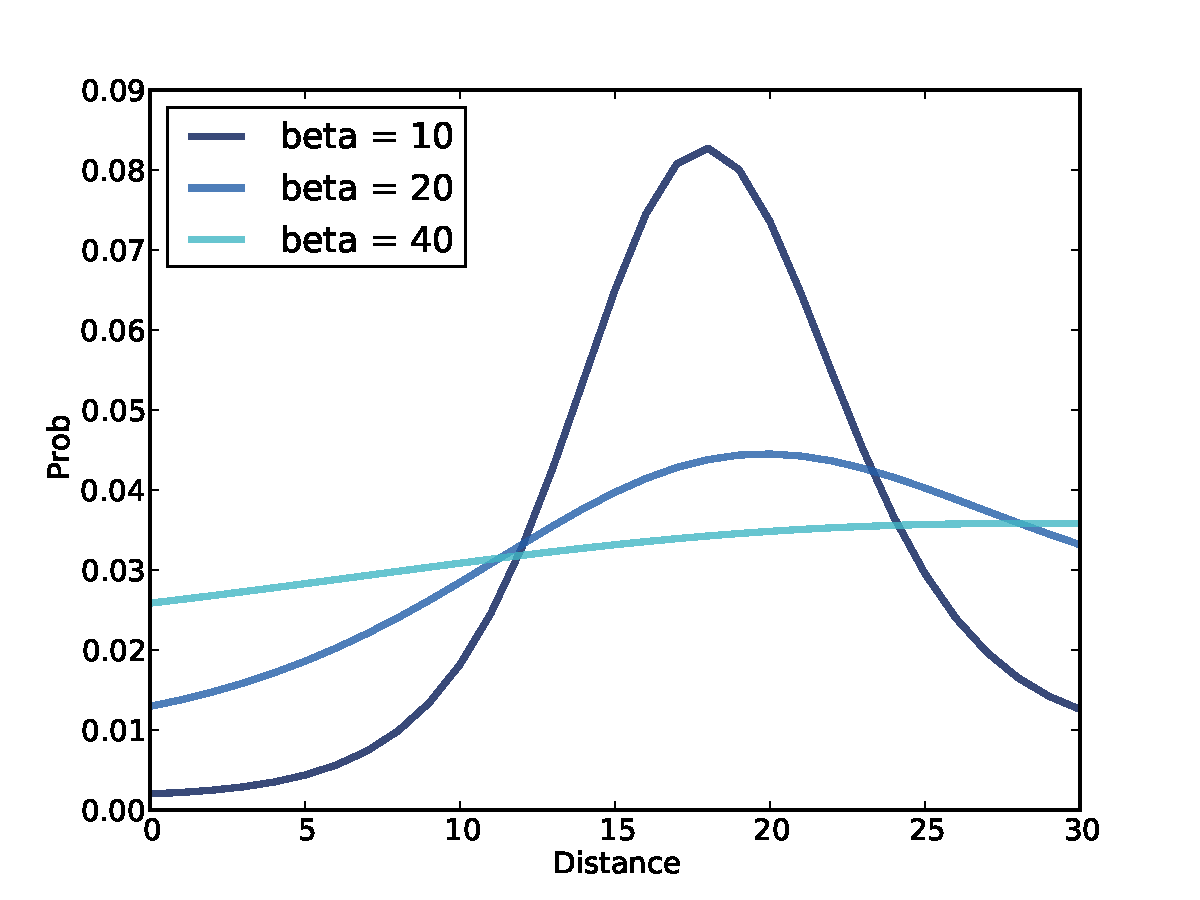
\includegraphics[height=2.5in]{figs/paintball3.pdf}}
\caption{Posterior distributions for {\tt alpha} conditioned on several values
of {\tt beta}.}
\label{fig.paintball3}
\end{figure}

The marginal distributions contain information about the variables
independently, but they do not capture the dependence between
variables, if any.
\index{independence}
\index{dependence}

One way to visualize dependence is by computing {\bf conditional
distributions}.  {\tt thinkbayes.Joint} provides a method that
does that:
\index{conditional distribution}
\index{Joint}

\begin{code}
    def Conditional(self, i, j, val):
        pmf = Pmf()
        for vs, prob in self.Items():
            if vs[j] != val: continue
            pmf.Incr(vs[i], prob)

        pmf.Normalize()
        return pmf
\end{code}

Again, {\tt i} is the index of the variable we want; {\tt j}
is the index of the conditioning variable, and {\tt val} is the
conditional value.

The result is the distribution of the $i$th variable under the
condition that the $j$th variable is {\tt val}.

For example, the following code computes the conditional distributions
of {\tt alpha} for a range of values of {\tt beta}:

\begin{code}
    betas = [10, 20, 40]

    for beta in betas:
        cond = suite.Conditional(0, 1, beta)
\end{code}

Figure~\ref{fig.paintball3} shows the results, which we could
fully describe as ``posterior conditional marginal distributions.''
Whew!

If the variables were independent, the conditional distributions would
all be the same.  Since they are all different, we can tell the
variables are dependent.  For example, if we know (somehow) that {\tt
  beta = 10}, the conditional distribution of {\tt alpha} is fairly
narrow.  For larger values of {\tt beta}, the distribution of
{\tt alpha} is wider.
\index{dependence}
\index{independence}


\section{Credible intervals}

\begin{figure}
% paintball.py
\centerline{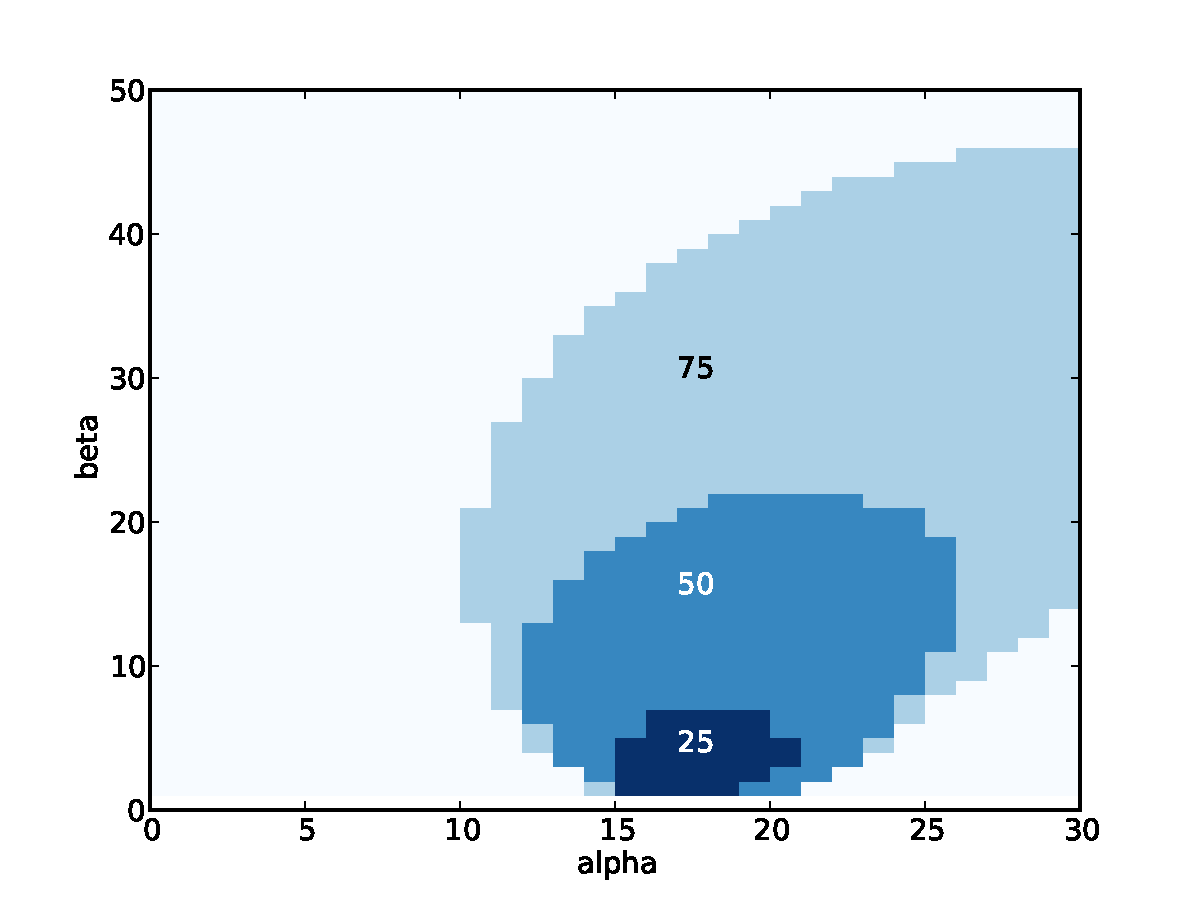
\includegraphics[height=2.5in]{figs/paintball5.pdf}}
\caption{Credible intervals for the coordinates of the opponent.}
\label{fig.paintball5}
\end{figure}

Another way to visualize the posterior joint distribution is to
compute credible intervals.  When we looked at credible intervals
in Section~\ref{credible},
I skipped over a subtle point: for a given distribution, there
are many intervals with the same level of credibility.  For example,
if you want a 50\% credible interval, you could choose any set of
values whose probability adds up to 50\%.

When the values are one-dimensional, it is most common to choose
the {\bf central credible interval}; for example, the central 50\%
credible interval contains all values between the 25th and 75th
percentiles.
\index{central credible interval}

In multiple dimensions it is less obvious what the right credible
interval should be.  The best choice might depend on context, but
one common choice is the maximum likelihood credible interval, which
contains the most likely values that add up to 50\% (or some other
percentage).
\index{maximum likelihood}

{\tt thinkbayes.Joint} provides a method that computes maximum
likelihood credible intervals. 
\index{Joint}

\begin{code}
# class Joint:

    def MaxLikeInterval(self, percentage=90):
        interval = []
        total = 0

        t = [(prob, val) for val, prob in self.Items()]
        t.sort(reverse=True)

        for prob, val in t:
            interval.append(val)
            total += prob
            if total >= percentage/100.0:
                break

        return interval
\end{code}

The first step is to make a list of the values in the suite,
sorted in descending order by probability.  Next we traverse the
list, adding each value to the interval, until the total
probability exceeds {\tt percentage}.  The result is a list
of values from the suite.  Notice that this set of values
is not necessarily contiguous.

To visualize the intervals, I wrote a function that ``colors''
each value according to how many intervals it appears in:

\begin{code}
def MakeCrediblePlot(suite):
    d = dict((pair, 0) for pair in suite.Values())

    percentages = [75, 50, 25]
    for p in percentages:
        interval = suite.MaxLikeInterval(p)
        for pair in interval:
            d[pair] += 1

    return d
\end{code}

{\tt d} is a dictionary that maps from each value in the suite
to the number of intervals it appears in.  The loop computes intervals
for several percentages and modifies {\tt d}.

Figure~\ref{fig.paintball5} shows the result.  The 25\% credible
interval is the darkest region near the bottom wall.  For higher
percentages, the credible interval is bigger, of course, and skewed
toward the right side of the room.


\section{Discussion}

This chapter shows that the Bayesian framework from the previous
chapters can be extended to handle a two-dimensional parameter space.
The only difference is that each hypothesis is represented by
a tuple of parameters.

I also presented {\tt Joint}, which is a parent class that provides
methods that apply to joint distributions:
{\tt Marginal}, {\tt Conditional}, and {\tt MakeLikeInterval}.
In object-oriented terms,
{\tt Joint} is a mixin (see \url{http://en.wikipedia.org/wiki/Mixin}).
\index{Joint}

There is a lot of new vocabulary in this chapter, so let's review:

\begin{description}

\item[Joint distribution:] A distribution that represents all possible
  values in a multidimensional space and their probabilities.  The
  example in this chapter is a two-dimensional space made up of the
  coordinates {\tt alpha} and {\tt beta}.  The joint distribution
  represents the probability of each ({\tt alpha}, {\tt beta}) pair.

\item[Marginal distribution:] The distribution of one parameter in a
  joint distribution, treating the other parameters as unknown.  For
  example, Figure~\ref{fig.paintball2} shows the distributions of {\tt
    alpha} and {\tt beta} independently.

\item[Conditional distribution:] The distribution of one parameter in
  a joint distribution, conditioned on one or more of the other
  parameters.  Figure~\ref{fig.paintball3} shows several distributions for
  {\tt alpha}, conditioned on different values of {\tt beta}.

\end{description}

Given the joint distribution, you can compute marginal and conditional
distributions.  With enough conditional distributions, you could
re-create the joint distribution, at least approximately.  But given
the marginal distributions you cannot re-create the joint distribution
because you have lost information about the dependence between
variables.
\index{joint distribution}
\index{conditional distribution}
\index{marginal distribution}

If there are $n$ possible values for each of two parameters, most
operations on the joint distribution take time proportional to $n^2$.
If there are $d$ parameters, run time is proportional to $n^d$,
which quickly becomes impractical as the number of dimensions increases.

If you can process a million hypotheses in a reasonable amount of time,
you could handle two dimensions with 1000 values for each parameter,
or three dimensions with 100 values each, or six dimensions with 10
values each.

If you need more dimensions, or more values per dimension, there are
optimizations you can try.  I present an example
in Chapter~\ref{species}.

You can download the code in this chapter from
\url{http://thinkbayes.com/paintball.py}.
  For more information
see Section~\ref{download}.

\section{Exercises}

\begin{exercise}
In our simple model, the opponent is equally likely to shoot in any
direction.  As an exercise, let's consider improvements to this model.

The analysis in this chapter suggests that a shooter is most likely to
hit the closest wall.  But in reality, if the opponent is close to a
wall, he is unlikely to shoot at the wall because he is unlikely to
see a target between himself and the wall.

Design an improved model that takes this behavior
into account.  Try to find a model that is more realistic, but not
too complicated.
\end{exercise}





\chapter{Approximate Bayesian Computation}

\section{The Variability Hypothesis}

I have a soft spot for crank science.  Recently I visited Norumbega
Tower, which is an enduring monument to the crackpot theories of Eben
Norton Horsford, inventor of double-acting baking powder and fake
history.  But that's not what this chapter is about.
\index{crank science}
\index{Horsford, Eben Norton}

This chapter is about the Variability Hypothesis, which
\index{Variability Hypothesis}
\index{Meckel, Johann}

\begin{quote}
"originated in the early nineteenth century with Johann Meckel, who
  argued that males have a greater range of ability than females,
  especially in intelligence. In other words, he believed that most
  geniuses and most mentally retarded people are men. Because he
  considered males to be the 'superior animal,' Meckel concluded that
  females' lack of variation was a sign of inferiority."

From \url{http://en.wikipedia.org/wiki/Variability_hypothesis}.
\end{quote}

I particularly like that last part, because I suspect that if it turns
out that women are actually more variable, Meckel would take that as a
sign of inferiority, too.  Anyway, you will not be surprised to hear
that the evidence for the Variability Hypothesis is weak.
\index{evidence}

Nevertheless, it came up in my class recently when we looked at data
from the CDC's Behavioral Risk Factor Surveillance System (BRFSS),
specifically the self-reported heights of adult American men and women.
The dataset includes responses from 154407 men and 254722 women.
Here's what we found:
\index{Centers for Disease Control}
\index{CDC}
\index{BRFSS}
\index{Behavioral Risk Factor Surveillance System}

\begin{itemize}

\item The average height for men is 178 cm; the average height for
  women is 163 cm.  So men are taller, on average.  No surprise there.

\item For men the standard deviation is 7.7 cm; for women it is 7.3
  cm.  So in absolute terms, men's heights are more variable.

\item But to compare variability between groups, it is more meaningful
  to use the coefficient of variation (CV), which is the standard
  deviation divided by the mean.  It is a dimensionless measure of
  variability relative to scale.  For men CV is 0.0433; for women it
  is 0.0444.
\index{coefficient of variation}

\end{itemize}

That's very close, so we could conclude that this dataset provides
weak evidence against the Variability Hypothesis.  But we can use
Bayesian methods to make that conclusion more precise.  And answering
this question gives me a chance to demonstrate some techniques
for working with large datasets.
\index{height}

I will proceed in a few steps:

\begin{enumerate}

\item We'll start with the simplest implementation, but it only works
  for datasets smaller than 1000 values.

\item By computing probabilities under a log transform, we can scale
  up to the full size of the dataset, but the computation gets slow.

\item Finally, we speed things up substantially with Approximate
  Bayesian Computation, also known as ABC.

\end{enumerate}

You can download the code in this chapter from
\url{http://thinkbayes.com/variability.py}.
  For more information
see Section~\ref{download}.

\section{Mean and standard deviation}

In Chapter~\ref{paintball} we estimated two parameters simultaneously
using a joint distribution.  In this chapter we use the same
method to estimate the parameters of a Gaussian distribution:
the mean, {\tt mu}, and the standard deviation, {\tt sigma}.
\index{Gaussian distribution}

For this problem, I define a Suite called {\tt Height} that
represents a map from each {\tt mu, sigma} pair to its probability:

\begin{code}
class Height(thinkbayes.Suite, thinkbayes.Joint):

    def __init__(self, mus, sigmas):
        pairs = [(mu, sigma) 
                 for mu in mus
                 for sigma in sigmas]

        thinkbayes.Suite.__init__(self, pairs)
\end{code}

{\tt mus} is a sequence of possible values for {\tt mu}; {\tt sigmas}
is a sequence of values for {\tt sigma}.  The prior distribution
is uniform over all {\tt mu, sigma} pairs.
\index{Joint}
\index{joint distribution}

The likelihood function is easy.  Given hypothetical values
of {\tt mu} and {\tt sigma}, we compute the likelihood
of a particular value, {\tt x}.  That's what {\tt EvalGaussianPdf}
does, so all we have to do is use it:
\index{likelihood}

\begin{code}
# class Height

    def Likelihood(self, data, hypo):
        x = data
        mu, sigma = hypo
        like = thinkbayes.EvalGaussianPdf(x, mu, sigma)
        return like
\end{code}

If you have studied statistics from a mathematical perspective,
you know that when you evaluate a PDF, you get a probability
density.  In order to get a probability, you have to integrate
probability densities over some range.
\index{density}

But for our purposes, we don't need a probability; we just
need something proportional to the probability we want.
A probability density does that job nicely.

The hardest part of this problem turns
out to be choosing appropriate ranges for {\tt mus} and
{\tt sigmas}.  If the range is too small, we omit some
possibilities with non-negligible probability and get the
wrong answer.  If the range is too big, we get the right answer,
but waste computational power.

So this is an opportunity to use classical estimation to
make Bayesian techniques more efficient.  Specifically, we can use
classical estimators to find a likely location for {\tt mu} and {\tt
  sigma}, and use the standard errors of those estimates to choose a
likely spread.
\index{classical estimation}

If the true parameters of the distribution are $\mu$ and $\sigma$, and
we take a sample of $n$ values, an estimator of $\mu$ is the sample
mean, {\tt m}.

And an estimator of $\sigma$ is the sample standard
variance, {\tt s}.

The standard error of the estimated $\mu$ is $s / \sqrt{n}$
and the standard error of the estimated $\sigma$ is
$s / \sqrt{2 (n-1)}$.

Here's the code to compute all that:

\begin{code}
def FindPriorRanges(xs, num_points, num_stderrs=3.0):

    # compute m and s
    n = len(xs)
    m = numpy.mean(xs)
    s = numpy.std(xs)

    # compute ranges for m and s
    stderr_m = s / math.sqrt(n)
    mus = MakeRange(m, stderr_m, num_stderrs)

    stderr_s = s / math.sqrt(2 * (n-1))
    sigmas = MakeRange(s, stderr_s, num_stderrs)

    return mus, sigmas
\end{code}

{\tt xs} is the dataset.  \verb"num_points" is the desired number of
values in the range.  \verb"num_stderrs" is the width of the range on
each side of the estimate, in number of standard errors.

The return
value is a pair of sequences, {\tt mus} and {\tt sigmas}.

Here's {\tt MakeRange}:
\index{numpy}

\begin{code}
def MakeRange(estimate, stderr, num_stderrs):
    spread = stderr * num_stderrs
    array = numpy.linspace(estimate-spread,
                           estimate+spread,
                           num_points)
    return array
\end{code}

{\tt numpy.linspace} makes an array of equally spaced elements between
{\tt estimate-spread} and {\tt estimate+spread}, including both.
\index{linspace}


\section{Update}

Finally here's the code to make and update the suite:

\begin{code}
    mus, sigmas = FindPriorRanges(xs, num_points)
    suite = Height(mus, sigmas)
    suite.UpdateSet(xs)
    print suite.MaximumLikelihood()    
\end{code}

This process might seem bogus, because we use the data to choose the
range of the prior distribution, and then use the data again to do the
update.  In general, using the same data twice is, in fact, bogus.
\index{bogus}
\index{maximum likelihood}

But in this case it is ok.  Really.  We use the data to choose the
range for the prior, but only to avoid computing a lot of
probabilities that would have been very small anyway.  With
\verb"num_stderrs=4", the range is big enough to cover all values with
non-negligible likelihood.  After that, making it bigger has no effect
on the results.

In effect, the prior is uniform over all values 
of {\tt mu} and {\tt sigma}, but for computational efficiency
we ignore all the values that don't matter.

\section{The posterior distribution of CV}

Once we have the posterior joint distribution of {\tt mu} and {\tt
  sigma}, we can compute the distribution of CV for men and women, and
then the probability that one exceeds the other.

To compute the distribution of CV, we enumerate pairs of
{\tt mu} and {\tt sigma}:

\begin{code}
def CoefVariation(suite):
    pmf = thinkbayes.Pmf()
    for (mu, sigma), p in suite.Items():
        pmf.Incr(sigma/mu, p)
    return pmf
\end{code}

Then we use \verb"thinkbayes.PmfProbGreater" to compute the
probability that men are more variable.

The analysis itself is simple, but there are two more issues we
have to deal with:

\begin{enumerate}

\item As the size of the dataset increases, we run into a series of
  computational problems due to the limitations of floating-point
  arithmetic.

\item The dataset contains a number of extreme values that are almost
  certainly errors.  We will need to make the estimation process
  robust in the presence of these outliers.

\end{enumerate}

The following sections explain these problems and their solutions.


\section{Underflow}
\label{underflow}

If we select the first 100 values from the BRFSS dataset and run the
analysis I just described, it runs without errors and we get posterior
distributions that look reasonable.

If we select the first 1000 values and run the program again, we get
an error in \verb"Pmf.Normalize":

\begin{code}
ValueError: total probability is zero.
\end{code}

The problem is that we are using probability densities to compute
likelihoods, and densities from continuous distributions tend to be
small.  And if you take 1000 small values and multiply
them together, the result is very small.  In this case it is so small
it can't be represented by a floating-point number, so it gets rounded
down to zero, which is called {\bf underflow}.  And if all
probabilities in the distribution are 0, it's not a distribution any
more.
\index{underflow}

A possible solution is to renormalize the Pmf after each update,
or after each batch of 100.  That would work, but it would be slow.

A better alternative is to compute likelihoods under a log
transform.  That way, instead of multiplying small values, we can add
up log likelihoods.  {\tt Pmf} provides methods {\tt Log}, {\tt
  LogUpdateSet} and {\tt Exp} to make this process easy.
\index{logarithm}
\index{log transform}

{\tt Log} computes the log of the probabilities in a Pmf:

\begin{code}
# class Pmf

    def Log(self):
        m = self.MaxLike()
        for x, p in self.d.iteritems():
            if p:
                self.Set(x, math.log(p/m))
            else:
                self.Remove(x)
\end{code}

Before applying the log transform {\tt Log} uses {\tt MaxLike} to find
{\tt m}, the highest probability in the Pmf.  It divide all
probabilities by {\tt m}, so the highest probability gets normalized
to 1, which yields a log of 0.  The other log probabilities are all
negative.  If there are any values in the Pmf with probability 0, they
are removed.

While the Pmf is under a log transform, we can't use {\tt Update},
{\tt UpdateSet}, or {\tt Normalize}.  The result would be nonsensical;
if you try, Pmf raises an exception.
Instead, we have to use {\tt LogUpdate}
and {\tt LogUpdateSet}.  
\index{exception}

Here's the implementation of {\tt LogUpdateSet}:

\begin{code}
# class Suite

    def LogUpdateSet(self, dataset):
        for data in dataset:
            self.LogUpdate(data)
\end{code}

{\tt LogUpdateSet} loops through the data and calls {\tt LogUpdate}:

\begin{code}
# class Suite

    def LogUpdate(self, data):
        for hypo in self.Values():
            like = self.LogLikelihood(data, hypo)
            self.Incr(hypo, like)
\end{code}

{\tt LogUpdate} is just like {\tt Update} except that it calls
{\tt LogLikelihood} instead of {\tt Likelihood}, and {\tt Incr}
instead of {\tt Mult}.

Using log-likelihoods avoids the problem with underflow, but while
the Pmf is under the log transform, there's not much we can do with
it.  We have to use {\tt Exp} to invert the transform:

\begin{code}
# class Pmf

    def Exp(self):
        m = self.MaxLike()
        for x, p in self.d.iteritems():
            self.Set(x, math.exp(p-m))
\end{code}

If the log-likelihoods are large negative numbers, the resulting
likelihoods might underflow.  So {\tt Exp} finds the maximum
log-likelihood, {\tt m}, and shifts all the likelihoods up by {\tt m}.
The resulting distribution has a maximum likelihood of 1.  This
process inverts the log transform with minimal loss of precision.
\index{maximum likelihood}


\section{Log-likelihood}

Now all we need is {\tt LogLikelihood}.

\begin{code}
# class Height

    def LogLikelihood(self, data, hypo):
        x = data
        mu, sigma = hypo
        loglike = scipy.stats.norm.logpdf(x, mu, sigma)
        return loglike
\end{code}

{\tt norm.logpdf} computes the log-likelihood of the
Gaussian PDF.
\index{scipy}
\index{log-likelihood}


Here's what the whole update process looks like:

\begin{code}
    suite.Log()
    suite.LogUpdateSet(xs)
    suite.Exp()
    suite.Normalize()
\end{code}

To review, {\tt Log} puts the suite under a log transform.
{\tt LogUpdateSet} calls {\tt LogUpdate}, which calls
{\tt LogLikelihood}.  {\tt LogUpdate} uses {\tt Pmf.Incr},
because adding a log-likelihood is the same as multiplying
by a likelihood.

After the update, the log-likelihoods are large negative
numbers, so {\tt Exp} shifts them up before inverting the
transform, which is how we avoid underflow.

Once the suite is transformed back, the probabilities
are ``linear'' again, which means ``not logarithmic'',
so we can use {\tt Normalize} again.

Using this algorithm, we can process the entire dataset without
underflow, but it is still slow.  On my computer it might
take an hour.  We can do better.


\section{A little optimization}

This section uses math and computational optimization
to speed things up by a factor of 100.  But the following section
presents an algorithm that is even faster.  So if you want to
get right to the good stuff, feel free to skip this section.
\index{optimization}

{\tt Suite.LogUpdateSet} calls {\tt LogUpdate} once for each data
point.  We can speed it up by computing the log-likelihood of the entire
dataset at once.

We'll start with the Gaussian PDF:
%
\[ \frac{1}{\sigma \sqrt{2 \pi}} \exp \left[ -\frac{1}{2} \left( \frac{x-\mu}{\sigma} \right)^2 \right] \]
%
and compute the log (dropping the constant term):
%
\[ -\log \sigma -\frac{1}{2} \left( \frac{x-\mu}{\sigma} \right)^2 \]
%
Given a sequence of values, $x_i$, the total log-likelihood is
%
\[ \sum_i -\log \sigma - \frac{1}{2} \left( \frac{x_i-\mu}{\sigma} \right)^2 \]
%
Pulling out the terms that don't depend on $i$, we get
%
\[ -n \log \sigma - \frac{1}{2 \sigma^2} \sum_i (x_i - \mu)^2 \]
%
which we can translate into Python:

\begin{code}
# class Height

    def LogUpdateSetFast(self, data):
        xs = tuple(data)
        n = len(xs)

        for hypo in self.Values():
            mu, sigma = hypo
            total = Summation(xs, mu)
            loglike = -n * math.log(sigma) - total / 2 / sigma**2
            self.Incr(hypo, loglike)
\end{code}

By itself, this would be a small improvement, but it
creates an opportunity for a bigger one.  Notice that the
summation only depends on {\tt mu}, not {\tt sigma}, so we only
have to compute it once for each value of {\tt mu}.
\index{optimization}

To avoid recomputing, I factor out a function that computes the
summation, and {\bf memoize} it so it stores previously computed
results in a dictionary (see
\url{http://en.wikipedia.org/wiki/Memoization}): \index{memoization}

\begin{code}
def Summation(xs, mu, cache={}):
    try:
        return cache[xs, mu]
    except KeyError:
        ds = [(x-mu)**2 for x in xs]
        total = sum(ds)
        cache[xs, mu] = total
        return total
\end{code}

{\tt cache} stores previously computed sums.  The {\tt try} statement
returns a result from the cache if possible; otherwise it computes
the summation, then caches and returns the result.
\index{cache}

The only catch is that we can't use a list as a key in the cache, because
it is not a hashable type.  That's why {\tt LogUpdateSetFast} converts
the dataset to a tuple.

This optimization speeds up the computation by about a
factor of 100, processing the entire dataset (154~407 men and 254~722
women) in less than a minute on my not-very-fast computer.


\section{ABC}

But maybe you don't have that kind of time.  In that case, Approximate
Bayesian Computation (ABC) might be the way to go.  The motivation
behind ABC is that the likelihood of any particular dataset is:
\index{ABC}
\index{Approximate Bayesian Computation}

\begin{enumerate}

\item Very small, especially for large datasets, which is why we had
to use the log transform,

\item Expensive to compute, which is why we had to do so much
optimization, and

\item Not really what we want anyway.

\end{enumerate}

We don't really care about the likelihood of seeing the exact dataset
we saw.  Especially for continuous variables, we care about the
likelihood of seeing any dataset like the one we saw.

For example, in the Euro problem, we don't care about the order of
the coin flips, only the total number of heads and tails.  And in
the locomotive problem, we don't care about which particular trains were
seen, only the number of trains and the maximum of the serial numbers.
\index{locomotive problem}
\index{Euro problem}

Similarly, in the BRFSS sample, we don't really want to know the
probability of seeing one particular set of values (especially since
there are hundreds of thousands of them).  It is more
relevant to ask, ``If we sample 100,000 people from a population
with hypothetical values of $\mu$ and $\sigma$, what would be
the chance of collecting a sample with the observed mean and
variance?''
\index{BRFSS}

For samples from a Gaussian distribution, we can answer this question
efficiently because we can find the distribution of the sample
statistics analytically.  In fact, we already did it when we computed
the range of the prior.
\index{Gaussian distribution}

If you draw $n$ values from a Gaussian distribution with parameters
$\mu$ and $\sigma$, and compute the sample mean, $m$, the
distribution of $m$ is Gaussian
with parameters $\mu$ and $\sigma / \sqrt{n}$.

Similarly, the distribution of the sample standard deviation, $s$, is
Gaussian with parameters $\sigma$ and $\sigma / \sqrt{2 (n-1)}$.

\index{sample statistics}
We can use these sample distributions to compute the likelihood of the
sample statistics, $m$ and $s$, given hypothetical values
for $\mu$ and $\sigma$.  Here's a new version of \verb"LogUpdateSet"
that does it:

\begin{code}
    def LogUpdateSetABC(self, data):
        xs = data
        n = len(xs)

        # compute sample statistics
        m = numpy.mean(xs)
        s = numpy.std(xs)

        for hypo in sorted(self.Values()):
            mu, sigma = hypo

            # compute log likelihood of m, given hypo
            stderr_m = sigma / math.sqrt(n)
            loglike = EvalGaussianLogPdf(m, mu, stderr_m)

            #compute log likelihood of s, given hypo
            stderr_s = sigma / math.sqrt(2 * (n-1))
            loglike += EvalGaussianLogPdf(s, sigma, stderr_s)

            self.Incr(hypo, loglike)
\end{code}

On my computer this function processes the entire dataset in about a
second, and the result agrees with the exact result with about 5
digits of precision.


\section{Robust estimation}

\begin{figure}
% variability.py
\centerline{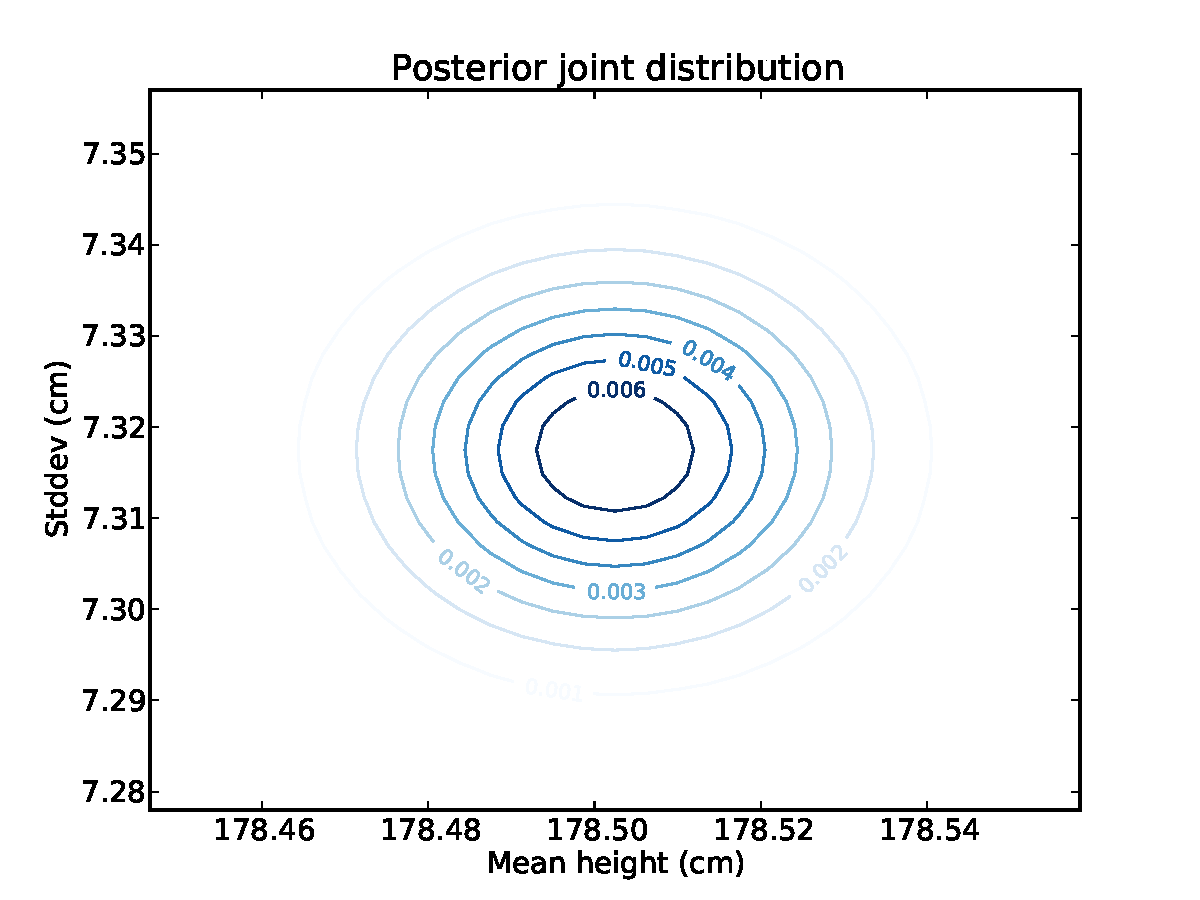
\includegraphics[height=2.5in]{figs/variability_posterior_male.pdf}}
\caption{Contour plot of the posterior joint distribution of
mean and standard deviation of height for men in the U.S.}
\label{fig.variability1}
\end{figure}

\begin{figure}
% variability.py
\centerline{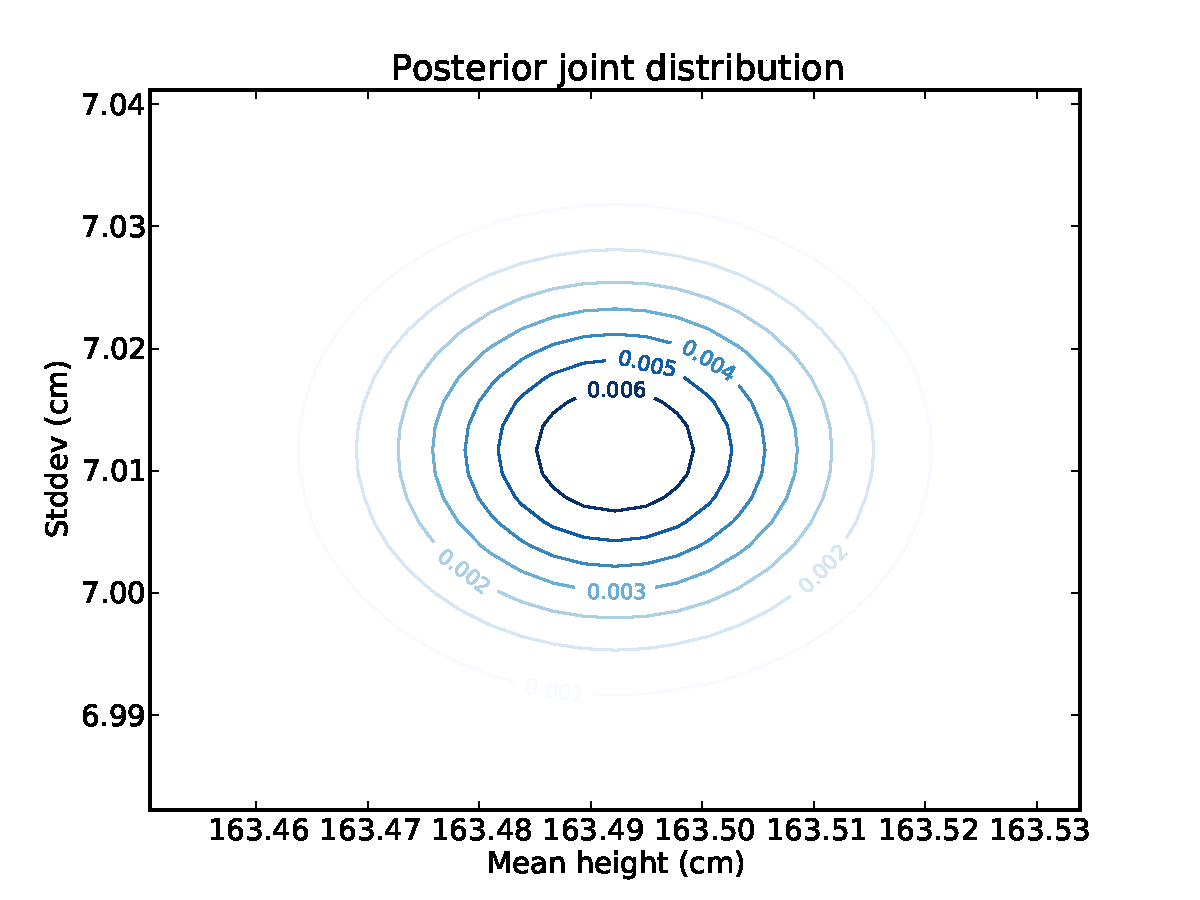
\includegraphics[height=2.5in]{figs/variability_posterior_female.pdf}}
\caption{Contour plot of the posterior joint distribution of
mean and standard deviation of height for women in the U.S.}
\label{fig.variability2}
\end{figure}

We are almost ready to look at results, but we have one more
problem to deal with.  There are a number of outliers in this
dataset that are almost certainly errors.  For example, there
are three adults with reported height of 61 cm, which would
place them among the shortest living adults in the world.
At the other end, there are four women with reported height
229 cm, just short of the tallest women in the world.

It is not impossible that these values are correct, but it is
unlikely, which makes it hard to know how to deal with them.
And we have to get
it right, because these extreme values have a disproportionate
effect on the estimated variability.

Because ABC is based on summary statistics, rather than the entire
dataset, we can make it more robust by choosing summary statistics
that are robust in the presence of outliers.  For example, rather
than use the sample mean and standard deviation, we could use the median
and inter-quartile range
(IQR), which is the difference between the 25th and 75th percentiles.
\index{summary statistic}
\index{robust estimation}
\index{inter-quartile range}
\index{IQR}

More generally, we could compute an inter-percentile range (IPR) that
spans any given fraction of the distribution, {\tt p}:

\begin{code}
def MedianIPR(xs, p):
    cdf = thinkbayes.MakeCdfFromList(xs)
    median = cdf.Percentile(50)

    alpha = (1-p) / 2
    ipr = cdf.Value(1-alpha) - cdf.Value(alpha)
    return median, ipr
\end{code}

{\tt xs} is a sequence of values.  {\tt p} is the desired range;
for example, {\tt p=0.5} yields the inter-quartile range.

{\tt MedianIPR} works by computing the CDF of {\tt xs},
then extracting the median and the difference between two
percentiles.

We can convert from {\tt ipr} to an estimate of {\tt sigma} using the
Gaussian CDF to compute the fraction of the distribution covered by a
given number of standard deviations.  For example, it is a well-known
rule of thumb that 68\% of a Gaussian distribution falls within one
standard deviation of the mean, which leaves 16\% in each tail.  If we
compute the range between the 16th and 84th percentiles, we expect the
result to be {\tt 2 * sigma}.  So we can estimate {\tt sigma} by
computing the 68\% IPR and dividing by 2.
\index{Gaussian distribution}

More generally we could use any number of {\tt sigmas}.
{\tt MedianS} performs the more general version of this
computation:

\begin{code}
def MedianS(xs, num_sigmas):
    half_p = thinkbayes.StandardGaussianCdf(num_sigmas) - 0.5

    median, ipr = MedianIPR(xs, half_p * 2)
    s = ipr / 2 / num_sigmas

    return median, s
\end{code}

Again, {\tt xs} is the sequence of values; \verb"num_sigmas" is the
number of standard deviations the results should be based on.  The
result is {\tt median}, which estimates $\mu$, and {\tt s}, which 
estimates $\sigma$.

Finally, in {\tt LogUpdateSetABC} we can replace the sample mean and
standard deviation with {\tt median} and {\tt s}.  And that pretty
much does it.

It might seem odd that we are using observed percentiles to
estimate $\mu$ and $\sigma$, but it is an example of the
flexibility of the Bayesian approach.  In effect we are asking,
``Given hypothetical values for $\mu$ and $\sigma$, and
a sampling process that has some chance of introducing errors,
what is the likelihood of generating a given set of sample
statistics?''

We are free to choose any sample statistics we like, up to a point:
$\mu$ and $\sigma$ determine the location and spread of
a distribution, so we need to choose statistics that capture those
characteristics.  For example, if we chose the 49th and 51st percentiles,
we would get very little information about spread, so it
would leave the estimate of $\sigma$ relatively unconstrained
by the data.  All values of {\tt sigma} would have nearly the
same likelihood of producing the observed values, so the posterior
distribution of {\tt sigma} would look a lot like the
prior.


\section{Who is more variable?}

\begin{figure}
% variability.py
\centerline{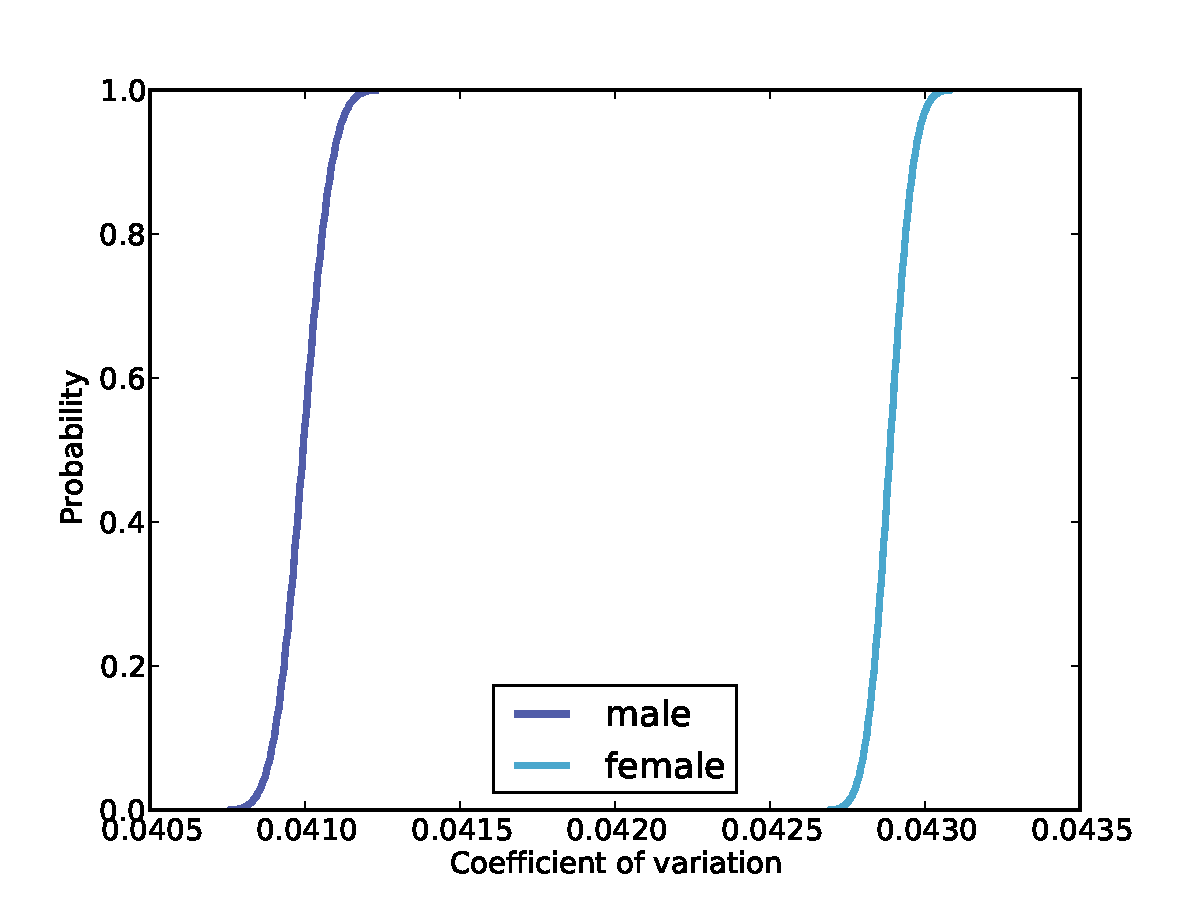
\includegraphics[height=2.5in]{figs/variability_cv.pdf}}
\caption{Posterior distributions of CV for men and women, based on
robust estimators.}
\label{fig.variability3}
\end{figure}

Finally we are ready to answer the question we started with: is the
coefficient of variation greater for men than for women?

Using ABC based on the median and IPR with \verb"num_sigmas=1", I
computed posterior joint distributions for {\tt mu} and {\tt
  sigma}.  Figures~\ref{fig.variability1} and ~\ref{fig.variability2}
show the results as a contour plot with {\tt mu} on the x-axis, {\tt
  sigma} on the y-axis, and probability on the z-axis.

For each joint distribution, I computed the posterior distribution of
CV.  Figure~\ref{fig.variability3} shows these distributions for men
and women.  The mean for men is 0.0410; for women it is 0.0429.
Since there is no overlap between the distributions, we conclude with
near certainty that
women are more variable in height than men.

So is that the end of the Variability Hypothesis?  Sadly, no.  It turns
out that this
result depends on the choice of the
inter-percentile range.  With \verb"num_sigmas=1", we conclude that
women are more variable, but with \verb"num_sigmas=2" we conclude
with equal confidence that men are more variable.

The reason for the difference is that there
are more men of short stature, and their distance from the mean is
greater.

So our evaluation of the Variability Hypothesis depends on the
interpretation of ``variability.''  With \verb"num_sigmas=1" we
focus on people near the mean.  As we increase
\verb"num_sigmas", we give more weight to the extremes.  

To decide which
emphasis is appropriate, we would need a more precise statement
of the hypothesis.  As it is, the Variability Hypothesis may be
too vague to evaluate.

Nevertheless, it helped
me demonstrate several new ideas and, I hope you agree,
it makes an interesting example.


\section{Discussion}

There are two ways you might think of ABC.  One interpretation
is that it is, as the name suggests, an approximation that is
faster to compute than the exact value.

But remember that Bayesian analysis is always
based on modeling decisions, which implies that there is no
``exact'' solution.  For any interesting
physical system there are many possible models, and each model
yields different results.  To interpret the results, we have to
evaluate the models.
\index{modeling}

So another interpretation of ABC is that it represents an alternative
model of the likelihood.  When we compute \p{D|H}, we are asking
``What is the likelihood of the data under a given hypothesis?''
\index{likelihood}

For large datasets, the likelihood of the data is very small, which
is a hint that we might not be asking the right question.  What
we really want to know is the likelihood of any outcome
like the data, where the definition of ``like'' is yet another
modeling decision.

The underlying idea of ABC is that two datasets are alike if they yield
the same summary statistics.  But in some cases, like the example in
this chapter, it is not obvious which summary statistics to choose.
\index{summary statistic}

You can download the code in this chapter from
\url{http://thinkbayes.com/variability.py}.
  For more information
see Section~\ref{download}.

\section{Exercises}

\begin{exercise}

An ``effect size'' is a statistic intended to measure the difference
between two groups (see
\url{http://en.wikipedia.org/wiki/Effect_size}).

For example, we could use data from the BRFSS to estimate the
difference in height between men and women.  By sampling values
from the posterior distributions of $\mu$ and
$\sigma$, we could generate the posterior distribution of this
difference.

But it might be better to use a dimensionless measure of effect
size, rather than a difference measured in cm.  One option is
to use divide through by the standard deviation (similar to what
we did with the coefficient of variation).

If the parameters for Group 1 are $(\mu_1, \sigma_1)$, and the
parameters for Group 2 are $(\mu_2, \sigma_2)$, the dimensionless
effect size is
%
\[ \frac{\mu_1 - \mu_2}{(\sigma_1 + \sigma_2)/2} \]
%
Write a function that takes joint distributions of
{\tt mu} and {\tt sigma} for two groups and returns
the posterior distribution of effect size.

Hint: if enumerating all pairs from the two distributions takes too
long, consider random sampling.

\end{exercise}



\chapter{Hypothesis Testing}
\label{hypotest}

\section{Back to the Euro problem}

In Section~\ref{euro} I presented a problem from MacKay's {\it Information
  Theory, Inference, and Learning Algorithms}:
\index{MacKay, David}

\begin{quote}
A statistical statement appeared in ``The Guardian" on Friday January 4, 2002:

  \begin{quote}
        When spun on edge 250 times, a Belgian one-euro coin came
        up heads 140 times and tails 110.  `It looks very suspicious
        to me,' said Barry Blight, a statistics lecturer at the London
        School of Economics.  `If the coin were unbiased, the chance of
        getting a result as extreme as that would be less than 7\%.'
        \end{quote}

But do these data give evidence that the coin is biased rather than fair?
\end{quote}

We estimated the probability that the coin would
land face up, but we didn't really answer MacKay's question:
Do the data give evidence that the coin is biased?
\index{Euro problem}
\index{evidence}

In Chapter~\ref{more} I proposed that data are in favor of
a hypothesis if the data are more likely under the hypothesis than
under the alternative or, equivalently, if the Bayes factor is greater
than 1.
\index{hypothesis testing}
\index{Bayes factor}

In the Euro example, we have two hypotheses to consider: I'll use
$F$ for the hypothesis that the coin is fair and $B$ for the hypothesis
that it is biased.
\index{fair coin}
\index{biased coin}

If the coin is fair, it is easy to compute the likelihood of the
data, \p{D|F}.  In fact, we already wrote the function
that does it.

\begin{code}
    def Likelihood(self, data, hypo):
        x = hypo / 100.0
        head, tails = data
        like = x**heads * (1-x)**tails
        return like
\end{code}

To use it we can
create a {\tt Euro} suite and invoke
{\tt Likelihood}:

\begin{code}
    suite = Euro()
    likelihood = suite.Likelihood(data, 50)
\end{code}

\p{D|F} is $5.5 \cdot 10^{-76}$, which doesn't tell us much except
that the probability of seeing any particular dataset is very small.
It takes two likelihoods to make a ratio, so we also have to
compute \p{D|B}.

It is not obvious how to compute the likelihood of $B$, because
it's not obvious what ``biased'' means.

One possibility is to cheat and look at the data before we define
the hypothesis.  In that case we would say that ``biased'' means that
the probability of heads is 140/250.

\begin{code}
    actual_percent = 100.0 * 140 / 250
    likelihood = suite.Likelihood(data, actual_percent)
\end{code}

This version of $B$ I call \verb"B_cheat"; the likelihood of
\verb"b_cheat" is $34 \cdot 10^{-76}$ and the likelihood ratio is
6.1.  So we would say that the data are evidence in favor of this
version of $B$.
\index{evidence}

But using the data to formulate the hypothesis
is obviously bogus.  By that definition, any dataset would
be evidence in favor of $B$, unless the observed percentage of heads
is exactly 50\%.
\index{bogus}

\section{Making a fair comparison}
\label{suitelike}

To make a legitimate comparison, we have to define $B$ without looking
at the data.  So let's try a different definition.  If you inspect
a Belgian Euro coin, you might notice that the ``heads'' side is more
prominent than the ``tails'' side.  You might expect the shape to 
have some effect on
$x$, but be unsure whether it makes heads more or less
likely.  So you might say ``I think the coin is biased so that
$x$ is either 0.6 or 0.4, but I am not sure which.''

We can think of this version, which I'll call \verb"B_two"
as a hypothesis made up of two
sub-hypotheses.  We can compute the likelihood for each
sub-hypothesis and then compute the average likelihood.

\begin{code}
    like40 = suite.Likelihood(data, 40)
    like60 = suite.Likelihood(data, 60)
    likelihood = 0.5 * like40 + 0.5 * like60
\end{code}

The likelihood ratio (or Bayes factor) for \verb"b_two" is 1.3, which
means the data provide weak evidence in favor of \verb"b_two".
\index{evidence}
\index{likelihood ratio}
\index{Bayes factor}

More generally, suppose you suspect that the coin is biased, but you
have no clue about the value of $x$.  In that case you might build a
Suite, which I call \verb"b_uniform", to represent sub-hypotheses from
0 to 100.

\begin{code}
    b_uniform = Euro(xrange(0, 101))
    b_uniform.Remove(50)
    b_uniform.Normalize()
\end{code}

I initialize \verb"b_uniform" with values from 0 to 100.
I removed the sub-hypothesis that $x$ is 50\%, because if
$x$ is 50\% the coin is fair, but it has almost no
effect on the result whether you remove it or not.

To compute the likelihood of
\verb"b_uniform" we compute the likelihood of each sub-hypothesis
and accumulate a weighted average.

\begin{code}
def SuiteLikelihood(suite, data):
    total = 0
    for hypo, prob in suite.Items():
        like = suite.Likelihood(data, hypo)
        total += prob * like
    return total
\end{code}

The likelihood ratio for \verb"b_uniform" is 0.47, which means
that the data are weak evidence against \verb"b_uniform",
compared to $F$.
\index{likelihood}

If you think about the computation performed by
\verb"SuiteLikelihood", you might notice that it is similar to an
update.  To refresh your memory, here's the {\tt Update} function:

\begin{code}
    def Update(self, data):
        for hypo in self.Values():
            like = self.Likelihood(data, hypo)
            self.Mult(hypo, like)
        return self.Normalize()
\end{code}

And here's {\tt Normalize}:

\begin{code}
    def Normalize(self):
        total = self.Total()
        
        factor = 1.0 / total
        for x in self.d:
            self.d[x] *= factor

        return total
\end{code}

The return value from {\tt Normalize} is the total of the
probabilities in the Suite, which is the average of the likelihoods
for the sub-hypotheses, weighted by the prior probabilities.  And {\tt
  Update} passes this value along, so instead of using {\tt
  SuiteLikelihood}, we could compute the likelihood of
\verb"b_uniform" like this:

\begin{code}
    likelihood = b_uniform.Update(data)
\end{code}



\section{The triangle prior}

In Chapter~\ref{more} we also considered a triangle-shaped prior that
gives higher probability to values of $x$ near 50\%.  If we think of
this prior as a suite of sub-hypotheses, we can compute its likelihood
like this:
\index{triangle distribution}

\begin{code}
    b_triangle = TrianglePrior()
    likelihood = b_triangle.Update(data)
\end{code}

The likelihood ratio for \verb"b_triangle" is 0.84, compared to $F$, so
again we would say that the data are weak evidence against $B$.
\index{evidence}

The following table shows the priors we have considered, the
likelihood of each, and the likelihood ratio (or Bayes factor)
relative to $F$.
\index{likelihood ratio}
\index{Bayes factor}

\begin{tabular}{|l|r|r|}
\hline
Hypothesis   & Likelihood & Bayes  \\
             & $\times 10^{-76}$ & Factor  \\
\hline
$F$              & 5.5   & --   \\
\verb"B_cheat"  & 34   &  6.1   \\
\verb"B_two"     & 7.4   &  1.3   \\
\verb"B_uniform"  & 2.6   &  0.47   \\
\verb"B_triangle"  & 4.6   &  0.84   \\
\hline
\end{tabular}

Depending on which definition we choose, the data might provide
evidence for or against the hypothesis that the coin is biased, but
in either case it is relatively weak evidence.

In summary, we can use Bayesian hypothesis testing to compare the
likelihood of $F$ and $B$, but we have to do some work to specify
precisely what $B$ means.  This specification depends on background
information about coins and their behavior when spun, so people
could reasonably disagree about the right definition.

My presentation of this example follows
David MacKay's discussion, and comes to the same conclusion.
You can download the code I used in this chapter from
\url{http://thinkbayes.com/euro3.py}.
  For more information
see Section~\ref{download}.

\section{Discussion}

The Bayes factor for \verb"B_uniform" is 0.47, which means
that the data provide evidence against this hypothesis, compared
to $F$.  In the previous section I characterized this evidence
as ``weak,'' but didn't say why.
\index{evidence}

Part of the answer is historical.  Harold Jeffreys, an early
proponent of Bayesian statistics, suggested a scale for
interpreting Bayes factors:

\begin{tabular}{|l|l|}
\hline
Bayes & Strength \\
Factor & \\
\hline
1 -- 3 & Barely worth mentioning \\
3 -- 10 & Substantial \\
10 -- 30 & Strong \\
30 -- 100 & Very strong \\
$>$ 100 & Decisive \\
\hline
\end{tabular}

In the example, the Bayes factor is 0.47 in favor of \verb"B_uniform",
so it is 2.1 in favor of $F$, which Jeffreys would consider ``barely
worth mentioning.''  Other authors have suggested variations on the
wording.  To avoid arguing about adjectives, we could think about odds
instead.

If your prior odds are 1:1, and you see evidence with Bayes
factor 2, your posterior odds are 2:1.  In terms of probability,
the data changed your degree of belief from 50\% to 66\%.  For
most real world problems, that change would be small relative
to modeling errors and other sources of uncertainty.

On the other hand, if you had seen evidence with Bayes
factor 100, your posterior odds would be 100:1 or more than 99\%.
Whether or not you agree that such evidence is ``decisive,''
it is certainly strong.

%TODO: postpone this section
\section{The beta distribution}
\label{beta}

\index{beta distribution}
There is one more optimization that solves this problem
even faster.

So far we have used a Pmf object to represent a discrete set of
values for {\tt x}.  Now we will use a continuous
distribution, specifically the beta distribution (see
\url{http://en.wikipedia.org/wiki/Beta_distribution}).
\index{continuous distribution}

The beta distribution is defined on the interval from 0 to 1
(including both), so it is a natural choice for describing
proportions and probabilities.  But wait, it gets better.

%TODO: explain the binomial distribution in the previous section

It turns out that if you do a Bayesian update with a binomial
likelihood function, which is what we did in the previous section, the beta
distribution is a {\bf conjugate prior}.  That means that if the prior
distribution for {\tt x} is a beta distribution, the posterior is also
a beta distribution.  But wait, it gets even better.
\index{binomial likelihood function}
\index{conjugate prior}

The shape of the beta distribution depends on two parameters, written
$\alpha$ and $\beta$, or {\tt alpha} and {\tt beta}.  If the prior
is a beta distribution with parameters {\tt alpha} and {\tt beta}, and
we see data with {\tt h} heads and {\tt t} tails, the posterior is a
beta distribution with parameters {\tt alpha+h} and {\tt beta+t}.  In
other words, we can do an update with two additions.
\index{parameter}

So that's great, but it only works if we can find a beta distribution
that is a good choice for a prior.  Fortunately, for many realistic
priors there is a beta distribution that is at least a good
approximation, and for a uniform prior there is a perfect match.  The
beta distribution with {\tt alpha=1} and {\tt beta=1} is uniform from
0 to 1.

Let's see how we can take advantage of all this.  
{\tt thinkbayes.py} provides 
a class that represents a beta distribution:
\index{Beta object}

\begin{code}
class Beta(object):

    def __init__(self, alpha=1, beta=1):
        self.alpha = alpha
        self.beta = beta
\end{code}

By default \verb"__init__" makes a uniform distribution.
{\tt Update} performs a Bayesian update:

\begin{code}
    def Update(self, data):
        heads, tails = data
        self.alpha += heads
        self.beta += tails
\end{code}

{\tt data} is a pair of integers representing the number of
heads and tails.

So we have yet another way to solve the Euro problem:

\begin{code}
    beta = thinkbayes.Beta()
    beta.Update((140, 110))
    print beta.Mean()
\end{code}

{\tt Beta} provides {\tt Mean}, which 
computes a simple function of {\tt alpha}
and {\tt beta}:

\begin{code}
    def Mean(self):
        return float(self.alpha) / (self.alpha + self.beta)
\end{code}

For the Euro problem the posterior mean is 56\%, which is the
same result we got using Pmfs.  

{\tt Beta} also provides {\tt EvalPdf}, which evaluates
the probability density
function (PDF)  of the beta distribution:
\index{probability density function}
\index{PDF}

\begin{code}
    def EvalPdf(self, x):
        return x**(self.alpha-1) * (1-x)**(self.beta-1)
\end{code}

Finally, {\tt Beta} provides {\tt MakePmf}, which
uses {\tt EvalPdf} to generate a discrete approximation
of the beta distribution.

%This expression might look familiar.  Here's {\tt
%  thinkbayes.EvalBinomialPmf}

%\begin{code}
%def EvalBinomialPmf(x, yes, no): 
%    return x**yes * (1-x)**no
%\end{code}

%It's the same function, but in {\tt EvalPdf}, we think of {\tt x} as a
%random variable and {\tt alpha} and {\tt beta} as parameters; in {\tt
%  EvalBinomialPmf}, {\tt x} is the parameter, and {\tt yes} and {\tt
%  no} are random variables.  Distributions like these that share the
%same PDF are called {\bf conjugate distributions}.
%\index{conjugate distribution}


\section{Exercises}

\begin{exercise}
Some people believe in the existence of extra-sensory
perception (ESP); for example, the ability of some people to guess
the value of an unseen playing card with probability better
than chance.
\index{ESP}
\index{extra-sensory perception}

What is your prior degree of belief in this kind of ESP?
Do you think it is as likely to exist as not?  Or are you
more skeptical about it?  Write down your prior odds.

Now compute the strength of the evidence it would take to
convince you that ESP is at least 50\% likely to exist.
What Bayes factor would be needed to make you 90\% sure
that ESP exists?

%TODO: figure out where to talk about Cromwell's rule
Also, notice that in a Bayesian update, we multiply
each prior probability by a likelihood, so if \p{H} is 0,
\p{H|D} is also 0, regardless of $D$.  In the Euro problem,
if you are convinced that \py{x} is less than 50\%, and you assign
probability 0 to all other hypotheses, no amount of data will
convince you otherwise.
\index{Euro problem}

This observation is the basis of {\bf Cromwell's rule}, which is the
recommendation that you should avoid giving a prior probability of
0 to any hypothesis that is even remotely possible
(see \url{http://en.wikipedia.org/wiki/Cromwell's_rule}).
\index{Cromwell's rule}

Cromwell's rule is named after Oliver Cromwell, who wrote, ``I beseech
you, in the bowels of Christ, think it possible that you may be
mistaken.''  For Bayesians, this turns out to be good advice (even if
it's a little overwrought).
\index{Cromwell, Oliver}
\end{exercise}


\begin{exercise}
Suppose that your answer to the previous question is 1000;
that is, evidence with Bayes factor 1000 in favor of ESP would
be sufficient to change your mind.

Now suppose that you read a paper in a respectable peer-reviewed
scientific journal that presents evidence with Bayes factor 1000 in
favor of ESP.  Would that change your mind?

If not, how do you resolve the apparent contradiction?
You might find it helpful to read about David Hume's article, ``Of
Miracles,'' at \url{http://en.wikipedia.org/wiki/Of_Miracles}.
\index{Hume, David}

\end{exercise}

\begin{exercise}

\url{https://en.wikipedia.org/wiki/Doomsday_argument}
\end{exercise}


\chapter{Evidence}
\label{evidence}

\section{Interpreting SAT scores}

Suppose you are the Dean of Admission at a small engineering
college in Massachusetts, and you are considering two candidates,
Alice and Bob, whose qualifications are similar in many ways,
with the exception that Alice got a higher score on the Math
portion of the SAT, a standardized test intended to measure
preparation for college-level work in mathematics.
\index{SAT}
\index{standardized test}

If Alice got 780 and Bob got a 740 (out of a possible 800), you might
want to know whether that difference is evidence that Alice is better
prepared than Bob, and what the strength of that evidence is.
\index{evidence}

Now in reality, both scores are very good, and both 
candidates are probably well prepared for college math.  So
the real Dean of Admission would probably suggest that we choose
the candidate who best demonstrates the other skills and
attitudes we look for in students.  But as an example of
Bayesian hypothesis testing, let's stick with a narrower question:
``How strong is the evidence that Alice is better prepared
than Bob?''

To answer that question, we need to make some modeling decisions.
I'll start with a simplification I know is wrong; then we'll come back
and improve the model.  I pretend, temporarily, that
all SAT questions are equally difficult.  Actually, the designers of
the SAT choose questions with a range of difficulty, because that
improves the ability to measure statistical differences between
test-takers.
\index{modeling}

But if we choose a model where all questions are equally difficult, we
can define a characteristic, \verb"p_correct", for each test-taker,
which is the probability of answering any question correctly.  This
simplification makes it easy to compute the likelihood of a given
score.


\section{The scale}

In order to understand SAT scores, we have to understand the scoring
and scaling process.  Each test-taker gets a raw score based on the
number of correct and incorrect questions.  The raw score is converted
to a scaled score in the range 200--800.
\index{scaled score}

In 2009, there were 54 questions on the math SAT.  The raw score
for each test-taker is the number of questions answered correctly
minus a penalty of $1/4$ point for each question answered incorrectly.

The College Board, which administers the SAT, publishes the
map from raw scores to scaled scores.  I have downloaded that
data and wrapped it in an Interpolator object that provides a forward
lookup (from raw score to scaled) and a reverse lookup (from scaled
score to raw).
\index{College Board}

You can download the code for this example from
\url{http://thinkbayes.com/sat.py}.
  For more information
see Section~\ref{download}.

\section{The prior}

The College Board also publishes the distribution of scaled scores
for all test-takers.  If we convert each scaled score to a raw score,
and divide by the number of questions, the result is an estimate
of \verb"p_correct".
So we can use the distribution of raw scores to model the
prior distribution of \verb"p_correct".

Here is the code that reads and processes the data:

\begin{code}
class Exam(object):

    def __init__(self):
        self.scale = ReadScale()
        scores = ReadRanks()
        score_pmf = thinkbayes.MakePmfFromDict(dict(scores))
        self.raw = self.ReverseScale(score_pmf)
        self.max_score = max(self.raw.Values())
        self.prior = DivideValues(self.raw, self.max_score)
\end{code}

{\tt Exam} encapsulates the information we have about the exam.
{\tt ReadScale} and {\tt ReadRanks} read files and return
objects that contain the data:
{\tt self.scale} is the {\tt Interpolator} that converts
from raw to scaled scores and back;  {\tt scores} is a list
of (score, frequency) pairs.

\verb"score_pmf" is the Pmf of
scaled scores.   {\tt self.raw} is the Pmf of raw scores, and
{\tt self.prior} is the Pmf of \verb"p_correct".

\begin{figure}
% sat.py
\centerline{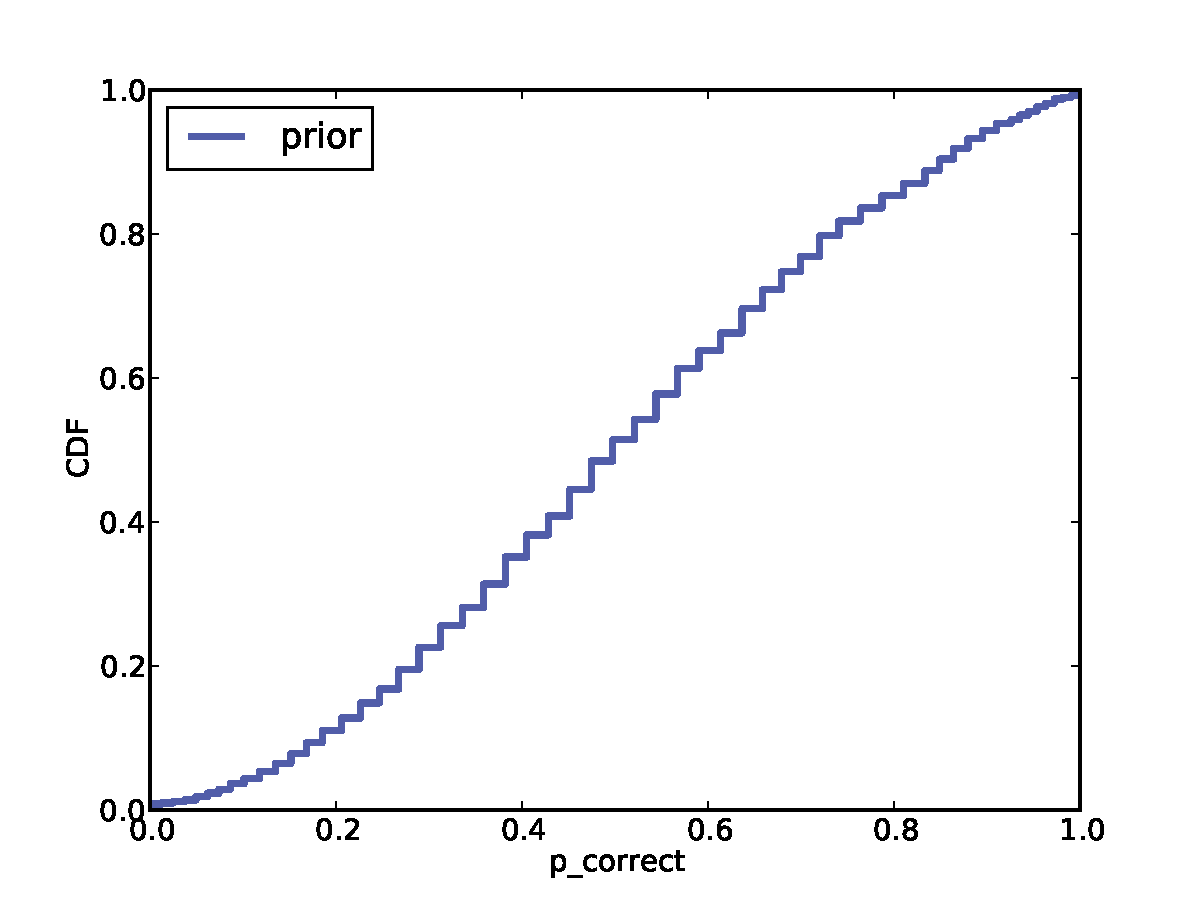
\includegraphics[height=2.5in]{figs/sat_prior.pdf}}
\caption{Prior distribution of {\tt p\_correct} for SAT test-takers.}
\label{fig.satprior}
\end{figure}

Figure~\ref{fig.satprior} shows the prior distribution of
\verb"p_correct".  This distribution is approximately Gaussian, but it
is compressed at the extremes.  By design, the SAT has the most power
to discriminate between test-takers within two standard deviations of
the mean, and less power outside that range.
\index{Gaussian distribution}

For each test-taker, I define a Suite called {\tt Sat} that
represents the distribution of \verb"p_correct".  Here's the definition:

\begin{code}
class Sat(thinkbayes.Suite):

    def __init__(self, exam, score):
        thinkbayes.Suite.__init__(self)

        self.exam = exam
        self.score = score

        # start with the prior distribution
        for p_correct, prob in exam.prior.Items():
            self.Set(p_correct, prob)

        # update based on an exam score
        self.Update(score)
\end{code}

\verb"__init__" takes an Exam object and a scaled score.  It makes a
copy of the prior distribution and then updates itself based on the
exam score.

As usual, we inherit {\tt Update} from {\tt Suite} and provide
{\tt Likelihood}:

\begin{code}
    def Likelihood(self, data, hypo):
        p_correct = hypo
        score = data

        k = self.exam.Reverse(score)
        n = self.exam.max_score
        like = thinkbayes.EvalBinomialPmf(k, n, p_correct)
        return like
\end{code}

{\tt hypo} is a hypothetical
value of \verb"p_correct", and {\tt data} is a scaled score.

To keep things simple, I interpret the raw score as the number of
correct answers, ignoring the penalty for wrong answers.  With
this simplification, the likelihood is given by the binomial
distribution, which computes the probability of $k$ correct
responses out of $n$ questions.
\index{binomial distribution}
\index{raw score}


\section{Posterior}

\begin{figure}
% sat.py
\centerline{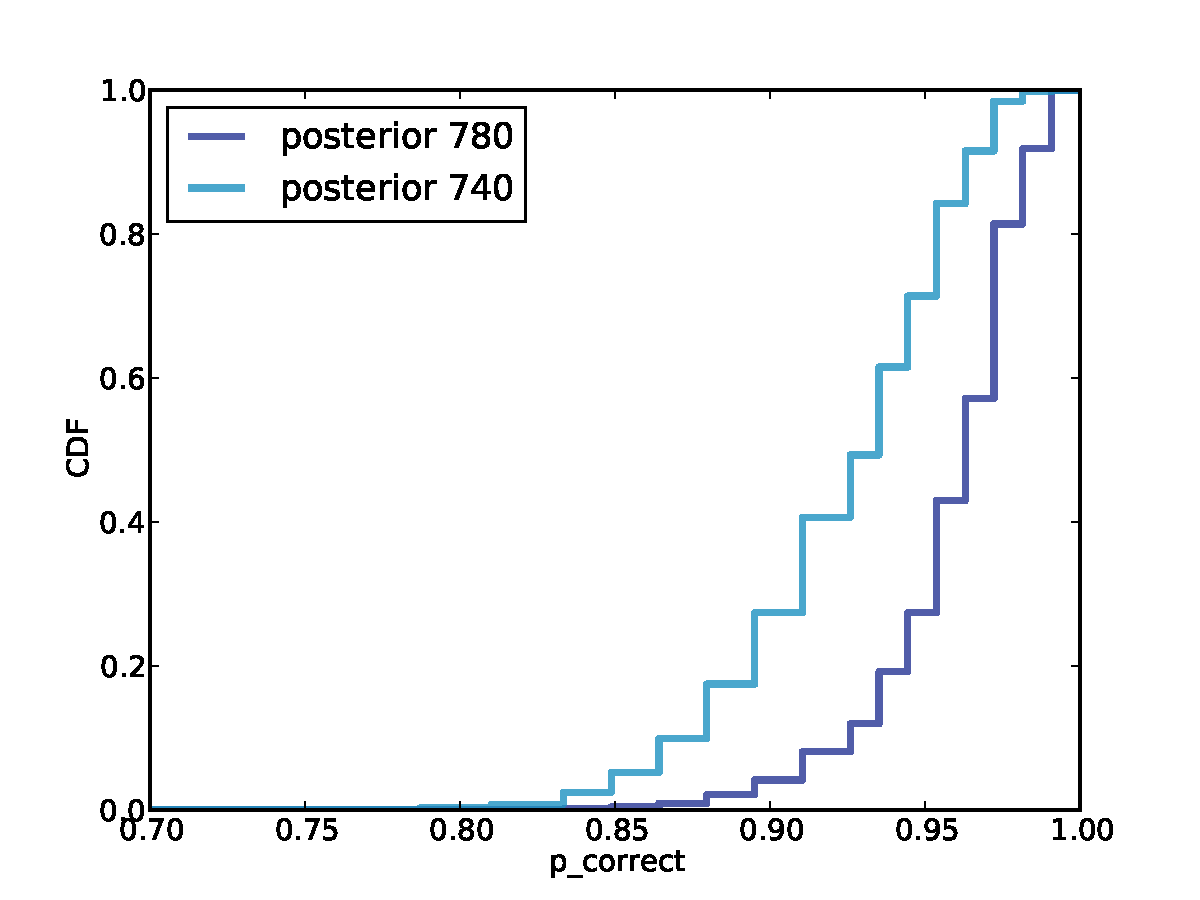
\includegraphics[height=2.5in]{figs/sat_posteriors_p_corr.pdf}}
\caption{Posterior distributions of {\tt p\_correct} for Alice and Bob.}
\label{fig.satposterior1}
\end{figure}

Figure~\ref{fig.satposterior1} shows the posterior distributions
of \verb"p_correct" for Alice and Bob based on their exam scores.
We can see that they overlap, so it is possible that \verb"p_correct"
is actually higher for Bob, but it seems unlikely.

Which brings us back to the original question, ``How strong is the
evidence that Alice is better prepared than Bob?''  We can use the
posterior distributions of \verb"p_correct" to answer this question.

To formulate the question in terms of Bayesian hypothesis testing,
I define two hypotheses:

\begin{itemize}

\item $A$: \verb"p_correct" is higher for Alice than for Bob.

\item $B$: \verb"p_correct" is higher for Bob than for Alice.

\end{itemize}

To compute the likelihood of $A$, we can enumerate all pairs of values
from the posterior distributions and add up the total probability of
the cases where \verb"p_correct" is higher for Alice than for Bob.
And we already have a function, \verb"thinkbayes.PmfProbGreater",
that does that.

So we can define a Suite that computes the posterior probabilities
of $A$ and $B$:

\begin{code}
class TopLevel(thinkbayes.Suite):

    def Update(self, data):
        a_sat, b_sat = data

        a_like = thinkbayes.PmfProbGreater(a_sat, b_sat)
        b_like = thinkbayes.PmfProbLess(a_sat, b_sat)
        c_like = thinkbayes.PmfProbEqual(a_sat, b_sat)

        a_like += c_like / 2
        b_like += c_like / 2

        self.Mult('A', a_like)
        self.Mult('B', b_like)

        self.Normalize()
\end{code}

Usually when we define a new Suite, we inherit {\tt Update}
and provide {\tt Likelihood}.  In this case I override {\tt Update},
because it is easier to evaluate the likelihood of both
hypotheses at the same time.

The data passed to {\tt Update} are Sat objects that represent
the posterior distributions of \verb"p_correct".

\verb"a_like" is the total probability that
\verb"p_correct" is higher for Alice; \verb"b_like" is that
probability that it is higher for Bob.

\verb"c_like" is the probability that they are ``equal,'' but this
equality is an artifact of the decision to model \verb"p_correct" with
a set of discrete values.  If we use more values, \verb"c_like"
is smaller, and in the extreme, if \verb"p_correct" is
continuous, \verb"c_like" is zero.  So I treat \verb"c_like" as
a kind of round-off error and split it evenly between \verb"a_like"
and \verb"b_like".

Here is the code that creates {\tt TopLevel} and updates it:

\begin{code}
    exam = Exam()
    a_sat = Sat(exam, 780)
    b_sat = Sat(exam, 740)

    top = TopLevel('AB')
    top.Update((a_sat, b_sat))
    top.Print()
\end{code}

The likelihood of $A$ is 0.79 and the likelihood of $B$ is 0.21.  The
likelihood ratio (or Bayes factor) is 3.8, which means that these test
scores are evidence that Alice is better than Bob at answering SAT
questions.  If we believed, before seeing the test scores, that $A$
and $B$ were equally likely, then after seeing the scores we should
believe that the probability of $A$ is 79\%, which means there is
still a 21\% chance that Bob is actually better prepared.
\index{likelihood ratio}
\index{Bayes factor}


\section{A better model}

Remember that the analysis we have done so far is based on
the simplification that all SAT questions are equally difficult.
In reality, some are easier than others, which means that the
difference between Alice and Bob might be even smaller.

But how big is the modeling error?  If it is small, we conclude
that the first model---based on the simplification that all questions
are equally difficult---is good enough.  If it's large,
we need a better model.
\index{modeling error}

In the next few sections, I develop a better model and 
discover (spoiler alert!) that the modeling error is small.  So if
you are satisfied with the simple model, you can skip to the next
chapter.  If you want to see how the more realistic model works,
read on...

\begin{itemize}

\item Assume that each test-taker has some 
  degree of {\tt efficacy}, which measures their
  ability to answer SAT questions.
\index{efficacy}

\item Assume that each question has some level of
  {\tt difficulty}.

\item Finally, assume that the chance that a test-taker answers a
  question correctly is related to {\tt efficacy} and {\tt difficulty}
  according to this function:

\begin{code}
def ProbCorrect(efficacy, difficulty, a=1):
    return 1 / (1 + math.exp(-a * (efficacy - difficulty)))
\end{code}

\end{itemize}

This function is a simplified version of the curve used in {\bf item
response theory}, which you can read about at
\url{http://en.wikipedia.org/wiki/Item_response_theory}.  {\tt
  efficacy} and {\tt difficulty} are considered to be on the same
scale, and the probability of getting a question right depends only on
the difference between them.
\index{item response theory}

When {\tt efficacy} and {\tt difficulty} are equal, the
probability of getting the question right is 50\%.  As
{\tt efficacy} increases, this probability approaches 100\%.
As it decreases (or as {\tt difficulty} increases), the
probability approaches 0\%.

Given the distribution of {\tt efficacy} across test-takers
and the distribution of {\tt difficulty} across questions, we
can compute the expected distribution of raw scores.  We'll do that
in two steps.  First, for a person with given {\tt efficacy},
we'll compute the distribution of raw scores.

\begin{code}
def PmfCorrect(efficacy, difficulties):
    pmf0 = thinkbayes.Pmf([0])

    ps = [ProbCorrect(efficacy, diff) for diff in difficulties]
    pmfs = [BinaryPmf(p) for p in ps]
    dist = sum(pmfs, pmf0)
    return dist
\end{code}

{\tt difficulties} is a list of difficulties, one for each question.
{\tt ps} is a list of probabilities, and {\tt pmfs} is a list of
two-valued Pmf objects; here's the function that makes them:

\begin{code}
def BinaryPmf(p):
    pmf = thinkbayes.Pmf()
    pmf.Set(1, p)
    pmf.Set(0, 1-p)
    return pmf
\end{code}

{\tt dist} is the sum of these Pmfs.  Remember from Section~\ref{addends}
that when we add up Pmf objects, the result is the distribution
of the sums.  In order to use Python's {\tt sum} to add up Pmfs,
we have to provide {\tt pmf0} which is the identity for Pmfs,
so {\tt pmf + pmf0} is always {\tt pmf}.

If we know a person's efficacy, we can compute their distribution
of raw scores.  For a group of people with a different efficacies, the
resulting distribution of raw scores is a mixture.  Here's the code
that computes the mixture:

\begin{code}
# class Exam:

    def MakeRawScoreDist(self, efficacies):
        pmfs = thinkbayes.Pmf()
        for efficacy, prob in efficacies.Items():
            scores = PmfCorrect(efficacy, self.difficulties)
            pmfs.Set(scores, prob)

        mix = thinkbayes.MakeMixture(pmfs)
        return mix
\end{code}

{\tt MakeRawScoreDist} takes {\tt efficacies}, which is a Pmf that
represents the distribution of efficacy across test-takers.  I assume
it is Gaussian with mean 0 and standard deviation 1.5.  This
choice is mostly arbitrary.  The probability of getting a question
correct depends on the difference between efficacy and difficulty, so
we can choose the units of efficacy and then calibrate the units of
difficulty accordingly.  \index{Gaussian distribution}

{\tt pmfs} is a meta-Pmf that contains one Pmf for each level of
efficacy, and maps to the fraction of test-takers at that level.  {\tt
  MakeMixture} takes the meta-pmf and computes the distribution of the
mixture (see Section~\ref{mixture}).  \index{meta-Pmf}
\index{MakeMixture}


\section{Calibration}

If we were given the distribution of difficulty, we could use
\verb"MakeRawScoreDist" to compute the distribution of raw scores.
But for us the problem is the other way around: we are given the
distribution of raw scores and we want to infer the distribution of
difficulty.

\begin{figure}
% sat.py
\centerline{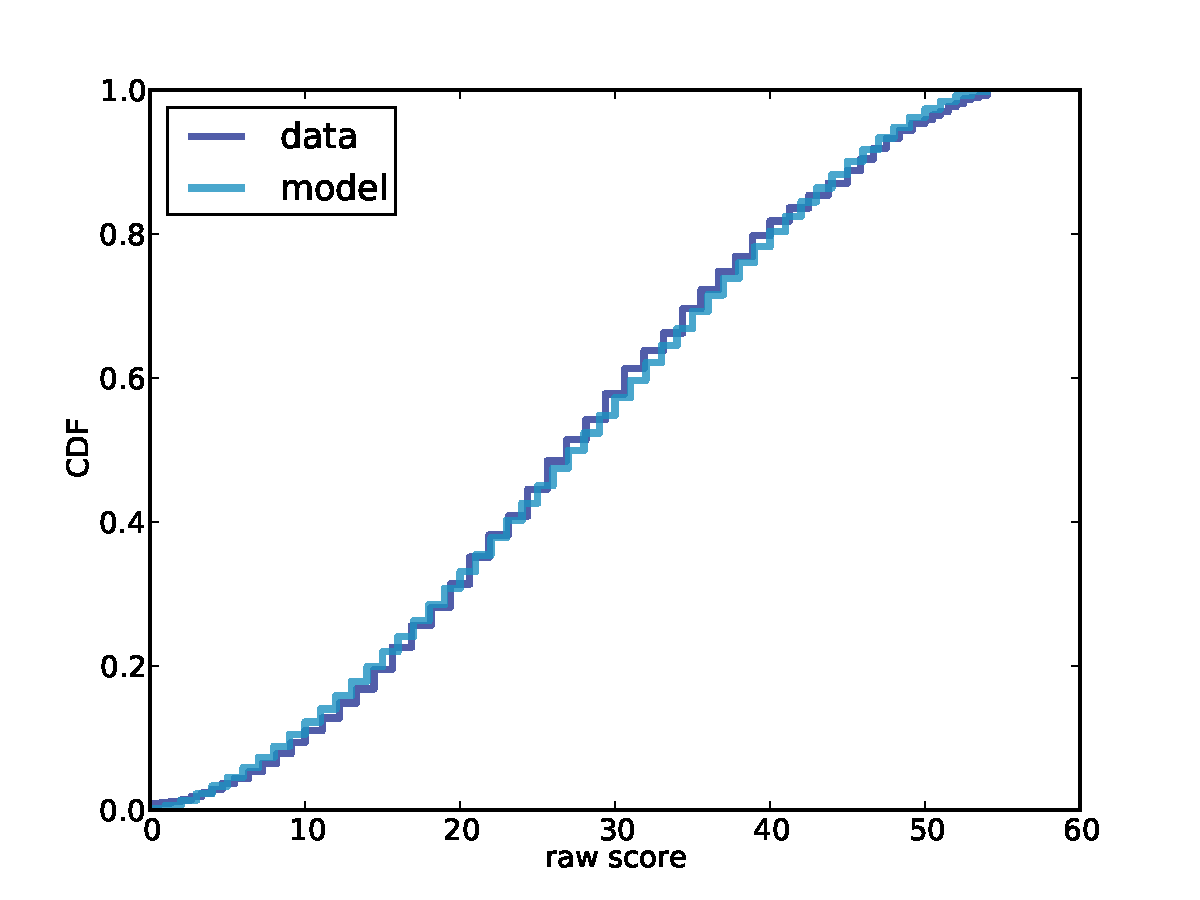
\includegraphics[height=2.5in]{figs/sat_calibrate.pdf}}
\caption{Actual distribution of raw scores and a model to fit it.}
\label{fig.satcalibrate}
\end{figure}

I assume that the distribution of difficulty is uniform with
parameters {\tt center} and {\tt width}.  {\tt MakeDifficulties}
makes a list of difficulties with these parameters.
\index{numpy}

\begin{code}
def MakeDifficulties(center, width, n):
    low, high = center-width, center+width
    return numpy.linspace(low, high, n)
\end{code}

By trying out a few combinations, I found that
{\tt center=-0.05} and {\tt width=1.8} yield a distribution
of raw scores similar to the actual data, as shown in
Figure~\ref{fig.satcalibrate}.
\index{calibration}

So, assuming that the distribution of difficulty is uniform,
its range is approximately
{\tt -1.85} to {\tt 1.75}, given that
efficacy is Gaussian with mean 0 and standard deviation 1.5.
\index{Gaussian distribution}

The following table shows the range of {\tt ProbCorrect} for
test-takers at different levels of efficacy:

\begin{tabular}{|r|r|r|r|}
\hline
           & \multicolumn{3}{|c|}{Difficulty} \\
\hline
Efficacy   & -1.85   &   -0.05   &      1.75  \\
\hline
3.00 &  0.99 &  0.95 &  0.78   \\
1.50 &  0.97 &  0.82 &  0.44   \\
0.00 &  0.86 &  0.51 &  0.15   \\
-1.50 &  0.59 &  0.19 &  0.04   \\
-3.00 &  0.24 &  0.05 &  0.01   \\
\hline
\end{tabular}

Someone with efficacy 3 (two standard deviations above
the mean) has a 99\% chance of answering the easiest questions on
the exam, and a 78\% chance of answering the hardest.  On the other
end of the range, someone two standard deviations below the mean
has only a 24\% chance of answering the easiest questions.


\section{Posterior distribution of efficacy}

\begin{figure}
% sat.py
\centerline{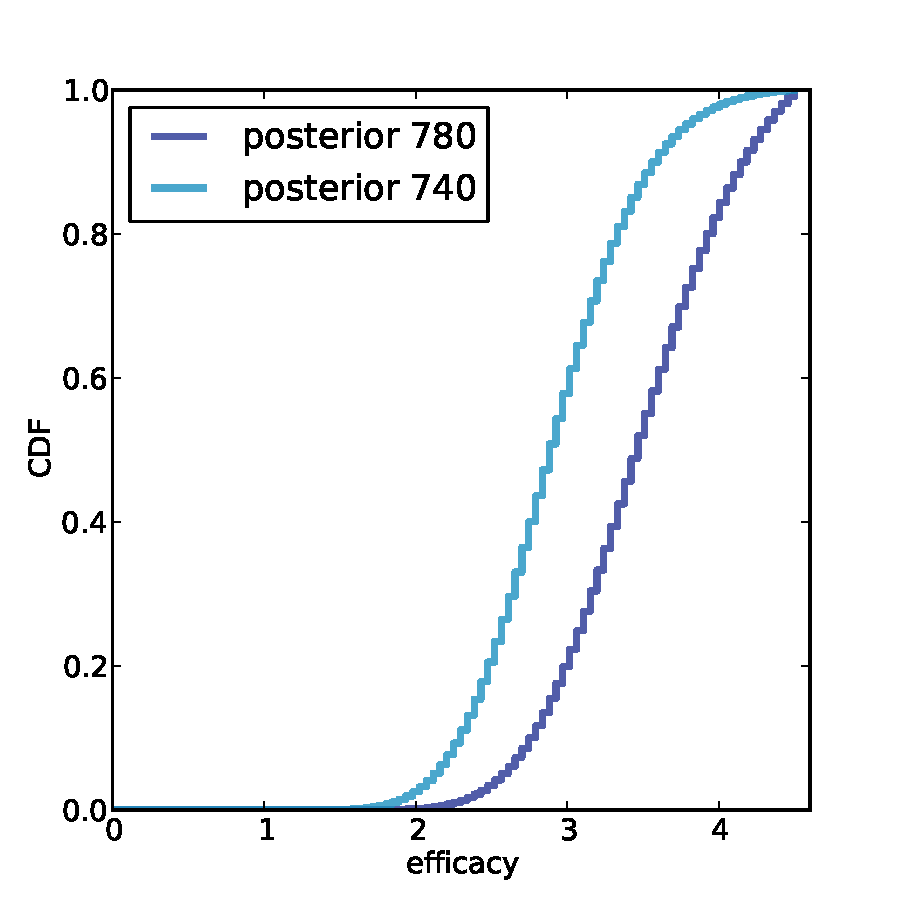
\includegraphics[height=2.5in]{figs/sat_posteriors_eff.pdf}}
\caption{Posterior distributions of efficacy for Alice and Bob.}
\label{fig.satposterior2}
\end{figure}

Now that the model is calibrated, we can compute the posterior
distribution of efficacy for Alice and Bob.  Here is a version of the
Sat class that uses the new model:

\begin{code}
class Sat2(thinkbayes.Suite):

    def __init__(self, exam, score):
        self.exam = exam
        self.score = score

        # start with the Gaussian prior
        efficacies = thinkbayes.MakeGaussianPmf(0, 1.5, 3)
        thinkbayes.Suite.__init__(self, efficacies)

        # update based on an exam score
        self.Update(score)
\end{code}

\verb"Update" invokes
\verb"Likelihood", which computes the likelihood of a given test score
for a hypothetical level of efficacy.

\begin{code}
    def Likelihood(self, data, hypo):
        efficacy = hypo
        score = data
        raw = self.exam.Reverse(score)

        pmf = self.exam.PmfCorrect(efficacy)
        like = pmf.Prob(raw)
        return like
\end{code}

{\tt pmf} is the distribution of raw scores for a test-taker
with the given efficacy; {\tt like} is the probability of
the observed score.

Figure~\ref{fig.satposterior2} shows the posterior distributions
of efficacy for Alice and Bob.  As expected, the location
of Alice's distribution is farther to the right, but again there
is some overlap.

Using {\tt TopLevel} again, we compare $A$, the
hypothesis that Alice's efficacy is higher, and $B$, the
hypothesis that Bob's is higher.  The likelihood ratio is
3.4, a bit smaller than what we got from the simple model (3.8).
So this model indicates that the data are evidence in favor
of $A$, but a little weaker than the previous estimate.

If our prior belief is that $A$ and $B$ are equally likely,
then in light of this evidence we would give $A$ a posterior
probability of 77\%, leaving a 23\% chance that Bob's efficacy
is higher.


\section{Predictive distribution}

The analysis we have done so far generates estimates for
Alice and Bob's efficacy, but since efficacy is not directly
observable, it is hard to validate the results.
\index{predictive distribution}

To give the model predictive power, we can use it to answer
a related question: ``If Alice and Bob take the math SAT
again, what is the chance that Alice will do better again?''

We'll answer this question in two steps:

\begin{itemize}

\item We'll use the posterior distribution of efficacy to
generate a predictive distribution of raw score for each test-taker.

\item We'll compare the two predictive distributions to compute
the probability that Alice gets a higher score again.

\end{itemize}

We already have most of the code we need.  To compute
the predictive distributions, we can use \verb"MakeRawScoreDist" again:

\begin{code}
    exam = Exam()
    a_sat = Sat(exam, 780)
    b_sat = Sat(exam, 740)

    a_pred = exam.MakeRawScoreDist(a_sat)
    b_pred = exam.MakeRawScoreDist(b_sat)
\end{code}

Then we can find the likelihood that Alice does better on the second
test, Bob does better, or they tie:

\begin{code}
    a_like = thinkbayes.PmfProbGreater(a_pred, b_pred)
    b_like = thinkbayes.PmfProbLess(a_pred, b_pred)
    c_like = thinkbayes.PmfProbEqual(a_pred, b_pred)
\end{code}

The probability that Alice does better on the second exam is 63\%,
which means that Bob has a 37\% chance of doing as well or better.

Notice that we have more confidence about Alice's efficacy than we do
about the outcome of the next test.  The posterior odds are 3:1 that
Alice's efficacy is higher, but only 2:1 that Alice will do better on
the next exam.


\section{Discussion}

\begin{figure}
% sat.py
\centerline{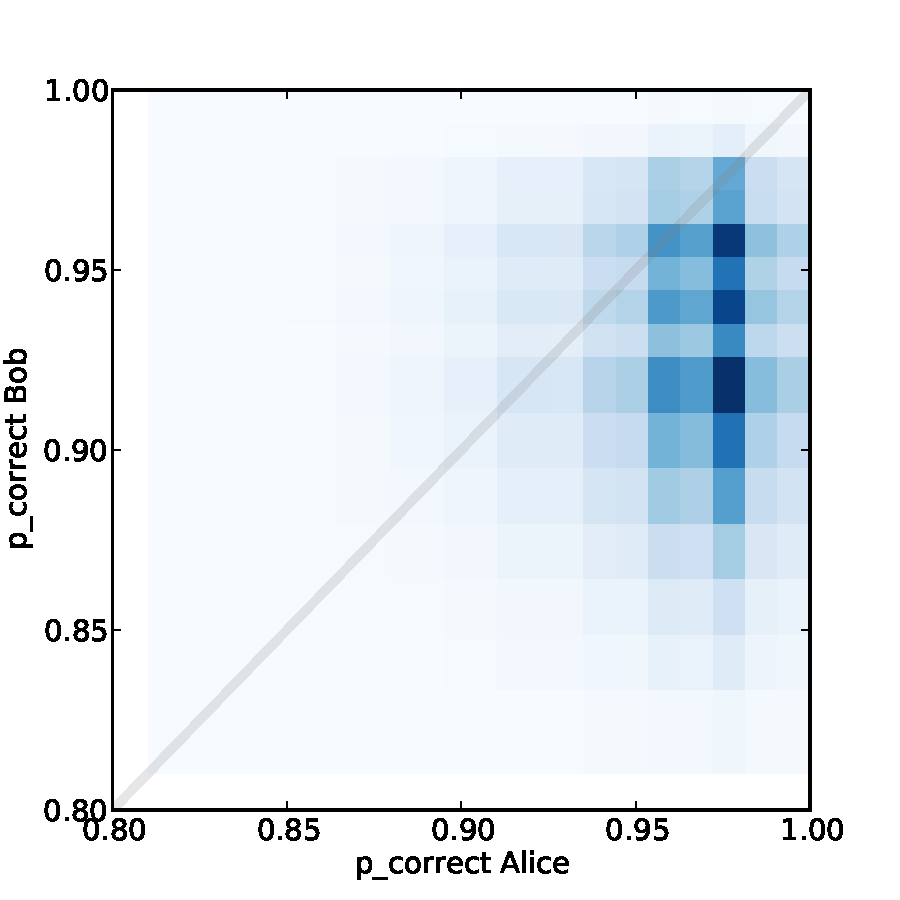
\includegraphics[height=2.5in]{figs/sat_joint.pdf}}
\caption{Joint posterior distribution of {\tt p\_correct} for Alice and Bob.}
\label{fig.satjoint}
\end{figure}

We started this chapter with the question,
``How strong is the evidence that Alice is better prepared
than Bob?''  On the face of it, that sounds like we want to
test two hypotheses: either Alice is more prepared or Bob is.

But in order to compute likelihoods for these hypotheses, we
have to solve an estimation problem.  For each test-taker
we have to find the posterior distribution of either
\verb"p_correct" or \verb"efficacy".

Values like this are called {\bf nuisance parameters} because
we don't care what they are, but we have
to estimate them to answer the question we care about.
\index{nuisance parameter}

One way to visualize the analysis we did in this chapter is
to plot the space of these parameters.  \verb"thinkbayes.MakeJoint"
takes two Pmfs, computes their joint distribution, and returns
a joint pmf of each possible pair of values and its probability.

\begin{code}
def MakeJoint(pmf1, pmf2):
    joint = Joint()
    for v1, p1 in pmf1.Items():
        for v2, p2 in pmf2.Items():
            joint.Set((v1, v2), p1 * p2)
    return joint
\end{code}

This function assumes that the two distributions are independent.
\index{joint distribution}
\index{independence}

Figure~\ref{fig.satjoint} shows the joint posterior distribution of
\verb"p_correct" for Alice and Bob.  The diagonal line indicates the
part of the space where \verb"p_correct" is the same for Alice and
Bob.  To the right of this line, Alice is more prepared; to the left,
Bob is more prepared.

In {\tt TopLevel.Update}, when we compute the likelihoods of $A$ and
$B$, we add up the probability mass on each side of this line.  For the
cells that fall on the line, we add up the total mass and split it
between $A$ and $B$.

The process we used in this chapter---estimating nuisance
parameters in order to evaluate the likelihood of competing
hypotheses---is a common Bayesian approach to problems like this.




\chapter{Simulation}

In this chapter I describe my solution to a problem posed
by a patient with a kidney tumor.  I think the problem is 
important and relevant to patients with these tumors
and doctors treating them.

And I think the solution is interesting because, although it
is a Bayesian approach to the problem, the use of Bayes's theorem
is implicit.  I present the solution and my code; at the end
of the chapter I will explain the Bayesian part.

If you want more technical detail than I present here, you can
read my paper on this work at \url{http://arxiv.org/abs/1203.6890}.


\section{The Kidney Tumor problem}

\index{Kidney tumor problem}
\index{Reddit}
I am a frequent reader and occasional contributor to the online statistics
forum at \url{http://reddit.com/r/statistics}.  In November 2011, I read
the following message:

\begin{quote}
"I have Stage IV Kidney Cancer and am trying to determine if the
  cancer formed before I retired from the military. ... Given the
  dates of retirement and detection is it possible to determine when
  there was a 50/50 chance that I developed the disease? Is it
  possible to determine the probability on the retirement date?  My
  tumor was 15.5 cm x 15 cm at detection. Grade II."
\end{quote}

I contacted the author of the message and got more information; I learned
that veterans get different benefits if it is "more likely than not"
that a tumor formed while they were in military service (among other
considerations).

Because renal tumors grow slowly, and often do not cause symptoms,
they are sometimes left untreated.  As a result, doctors can observe
the rate of growth for untreated tumors by comparing scans from the
same patient at different times.  Several papers have reported these
growth rates.

I collected data from a paper by Zhang et al\footnote{Zhang et al,
  Distribution of Renal Tumor Growth Rates Determined by Using Serial
  Volumetric CT Measurements, January 2009 {\it Radiology}, 250,
  137-144.}.  I contacted the authors to see if I could get raw data,
but they refused on grounds of medical privacy.  Nevertheless, I was
able to extract the data I needed by printing one of their graphs and
measuring it with a ruler.

\begin{figure}
% kidney.py
\centerline{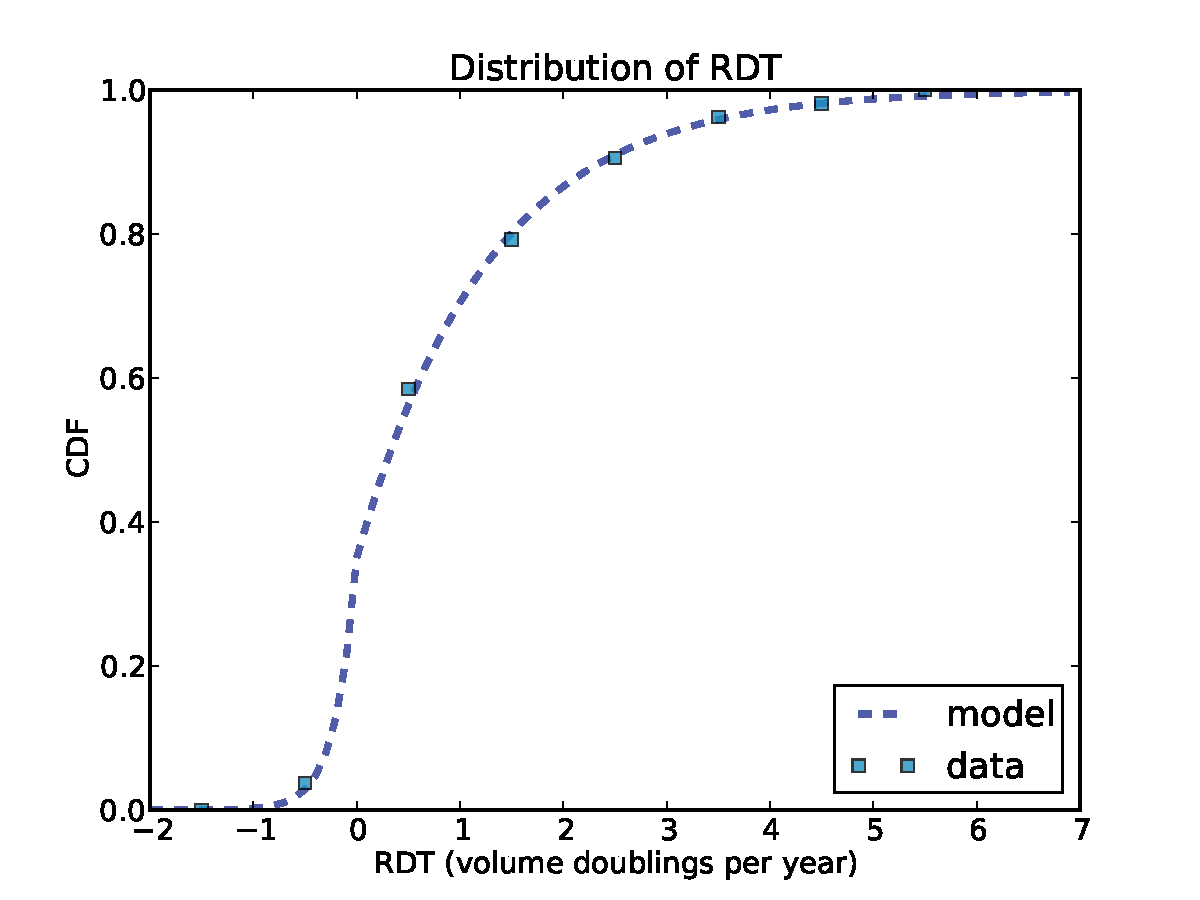
\includegraphics[height=2.5in]{figs/kidney2.pdf}}
\caption{CDF of RDT in doublings per year.}
\label{fig.kidney2}
\end{figure}

They report growth rates in reciprocal doubling time (RDT),
which is in units of doublings per year.  So a tumor with $RDT=1$
doubles in volume each year; with $RDT=2$ it quadruples in the same
time, and with $RDT=-1$, it halves.  Figure~\ref{fig.kidney2} shows the
distribution of RDT for 53 patients.
\index{doubling time}

The squares are the data points from the paper; the line is a model I
fit to the data.  The positive tail fits an exponential distribution
well, so I used a mixture of two exponentials.
\index{exponential distribution}
\index{mixture}



\section{A simple model}

It is usually a good idea to start with a simple model before
trying something more challenging.  Sometimes the simple model is
sufficient for the problem at hand, and if not, you can use it
to validate the more complex model.
\index{modeling}

For my simple model, I assume that tumors grow with a constant
doubling time, and that they are three-dimensional in the sense that
if the maximum linear measurement doubles, the volume is multiplied by
eight.

I learned from my correspondent that the time between his discharge
from the military and his diagnosis was 3291 days (about 9 years).
So my first calculation was, ``If this tumor grew at the median
rate, how big would it have been at the date of discharge?''

The median volume doubling time reported by Zhang et al is 811 days.
Assuming 3-dimensional geometry, the doubling time for a linear
measure is three times longer.

\begin{code}
    # time between discharge and diagnosis, in days 
    interval = 3291.0

    # doubling time in linear measure is doubling time in volume * 3
    dt = 811.0 * 3

    # number of doublings since discharge
    doublings = interval / dt

    # how big was the tumor at time of discharge (diameter in cm)
    d1 = 15.5
    d0 = d1 / 2.0 ** doublings
\end{code}

You can download the code in this chapter from
\url{http://thinkbayes.com/kidney.py}.  For more information
see Section~\ref{download}.

The result, {\tt d0}, is about 6 cm.  So if this tumor formed after
the date of discharge, it must have grown substantially faster than
the median rate.  Therefore I concluded that it is ``more likely than
not'' that this tumor formed before the date of discharge.

In addition, I computed the growth rate that would be implied
if this tumor had formed after the date of discharge.  If we
assume an initial size of 0.1 cm, we can compute the number of
doublings to get to a final size of 15.5 cm:

\begin{code}
    # assume an initial linear measure of 0.1 cm
    d0 = 0.1
    d1 = 15.5

    # how many doublings would it take to get from d0 to d1
    doublings = log2(d1 / d0)

    # what linear doubling time does that imply?
    dt = interval / doublings

    # compute the volumetric doubling time and RDT
    vdt = dt / 3
    rdt = 365 / vdt
\end{code}

{\tt dt} is linear doubling time, so {\tt vdt} is volumetric
doubling time, and {\tt rdt} is reciprocal doubling
time.

The number of doublings, in linear measure, is 7.3, which implies
an RDT of 2.4.  In the data from Zhang et al, only 20\% of tumors
grew this fast during a period of observation.  So again,
I concluded that is ``more likely than not'' that the tumor
formed prior to the date of discharge.

These calculations are sufficient to answer the question as
posed, and on behalf of my correspondent, I wrote a letter explaining
my conclusions to the Veterans' Benefit Administration.
\index{Veterans' Benefit Administration}

Later I told a friend, who is an oncologist, about my results.  He was
surprised by the growth rates observed by Zhang et al, and by what
they imply about the ages of these tumors.  He suggested that the
results might be interesting to researchers and doctors.

But in order to make them useful, I wanted a more general model
of the relationship between age and size.


\section{A more general model}

Given the size of a tumor at time of diagnosis, it would be most
useful to know the probability that the tumor formed before
any given date; in other words, the distribution of ages.
\index{modeling}
\index{simulation}

To find it, I run simulations of tumor growth to get the
distribution of size conditioned on age.  Then we can use
a Bayesian approach to get the
distribution of age conditioned on size.
\index{conditional distribution}

The simulation starts with a small tumor and runs these steps:

\begin{enumerate}

\item Choose a growth rate from the distribution of RDT.

\item Compute the size of the tumor at the end of an interval.

\item Record the size of the tumor at each interval.

\item Repeat until the tumor exceeds the maximum relevant size.

\end{enumerate}

For the initial size I chose 0.3 cm, because carcinomas smaller than
that are less likely to be invasive and less likely to have the blood
supply needed for rapid growth (see
\url{http://en.wikipedia.org/wiki/Carcinoma_in_situ}).  
\index{carcinoma}

I chose an interval of 245 days (about 8 months) because that is the
median time between measurements in the data source.

For the maximum size I chose 20 cm.  In the data source, the range of
observed sizes is 1.0 to 12.0 cm, so we are extrapolating beyond
the observed range at each end, but not by far, and not in a way
likely to have a strong effect on the results.

\begin{figure}
% kidney.py
\centerline{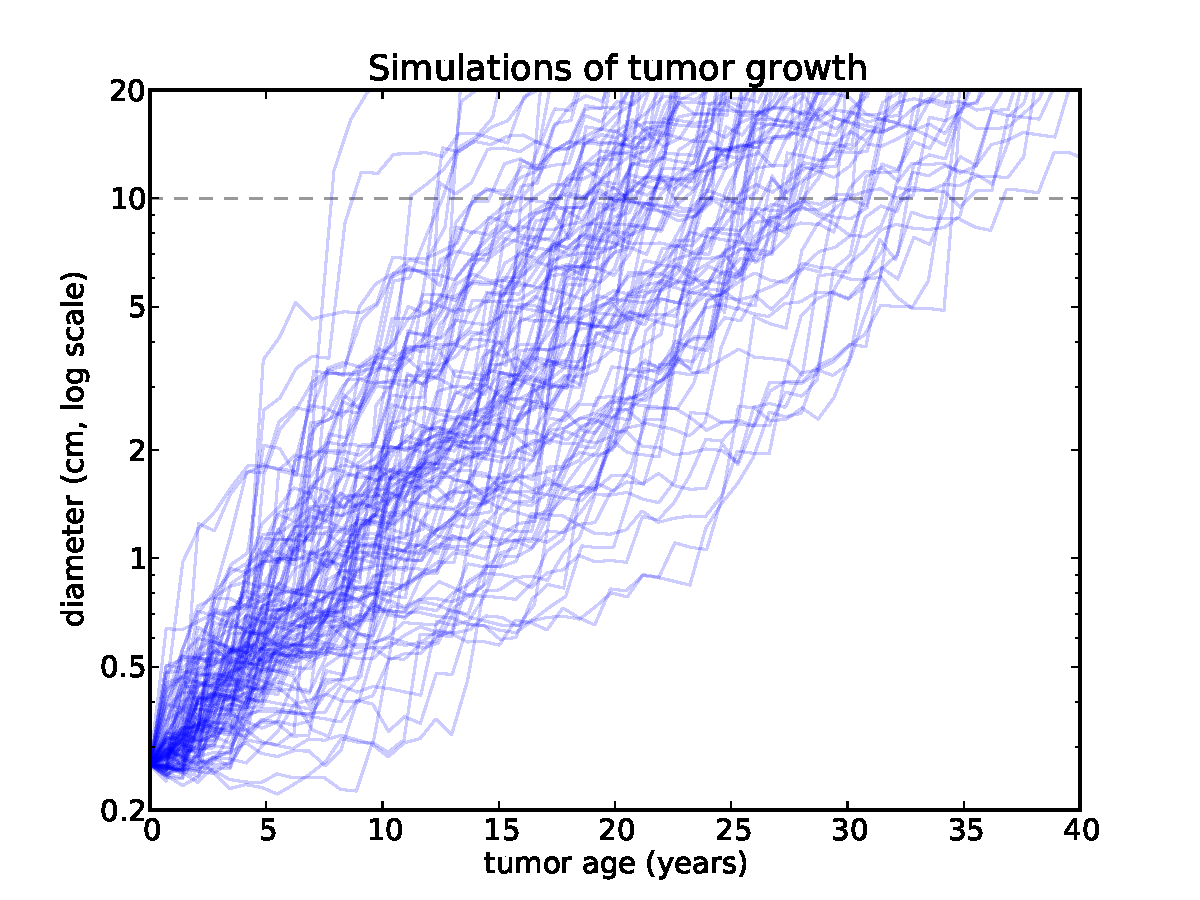
\includegraphics[height=2.5in]{figs/kidney4.pdf}}
\caption{Simulations of tumor growth, size vs. time.}
\label{fig.kidney4}
\end{figure}

The simulation is based on one big simplification:
the growth rate is chosen independently during each interval,
so it does not depend on age, size, or growth rate during
previous intervals.
\index{independence}

In Section~\ref{serial} I review these assumptions and
consider more detailed models.  But first let's look at some
examples.

Figure~\ref{fig.kidney4} shows 
the size of simulated tumors as a function of
age.  The dashed line at 10 cm shows the range of ages for tumors at
that size: the fastest-growing tumor gets there in 8 years; the
slowest takes more than 35.

I am presenting results in terms of linear measurements, but the
calculations are in terms of volume.  To convert from one to the
other, again, I use the volume of a sphere with the given
diameter.
\index{volume}
\index{sphere}


\section{Implementation}

Here is the kernel of the simulation:
\index{simulation}

\begin{code}
def MakeSequence(rdt_seq, v0=0.01, interval=0.67, vmax=Volume(20.0)):
    seq = v0,
    age = 0

    for rdt in rdt_seq:
        age += interval
        final, seq = ExtendSequence(age, seq, rdt, interval)
        if final > vmax:
            break

    return seq
\end{code}

\verb"rdt_seq" is an iterator that yields 
random values from the CDF of growth rate.
{\tt v0} is the initial volume in mL.  {\tt interval} is the time step
in years.  {\tt vmax} is the final volume corresponding to a linear
measurement of 20 cm.
\index{iterator}

{\tt Volume} converts from linear measurement in cm to volume
in mL, based on the simplification that the tumor is a sphere:

\begin{code}
def Volume(diameter, factor=4*math.pi/3):
    return factor * (diameter/2.0)**3
\end{code}

{\tt ExtendSequence} computes the volume of the tumor at the
end of the interval.

\begin{code}
def ExtendSequence(age, seq, rdt, interval):
    initial = seq[-1]
    doublings = rdt * interval
    final = initial * 2**doublings
    new_seq = seq + (final,)
    cache.Add(age, new_seq, rdt)
    
    return final, new_seq
\end{code}

{\tt age} is the age of the tumor at the end of the interval.
{\tt seq} is a tuple that contains the volumes so far.  {\tt rdt} is
the growth rate during the interval, in doublings per year.
{\tt interval} is the size of the time step in years.

The return values are {\tt final}, the volume of the
tumor at the end of the interval, and \verb"new_seq", a new
tuple containing the volumes in {\tt seq} plus the new volume
{\tt final}.

{\tt Cache.Add} records the age and size of each tumor at the end
of each interval, as explained in the next section.
\index{cache}


\section{Caching the joint distribution}

\begin{figure}
% kidney.py
\centerline{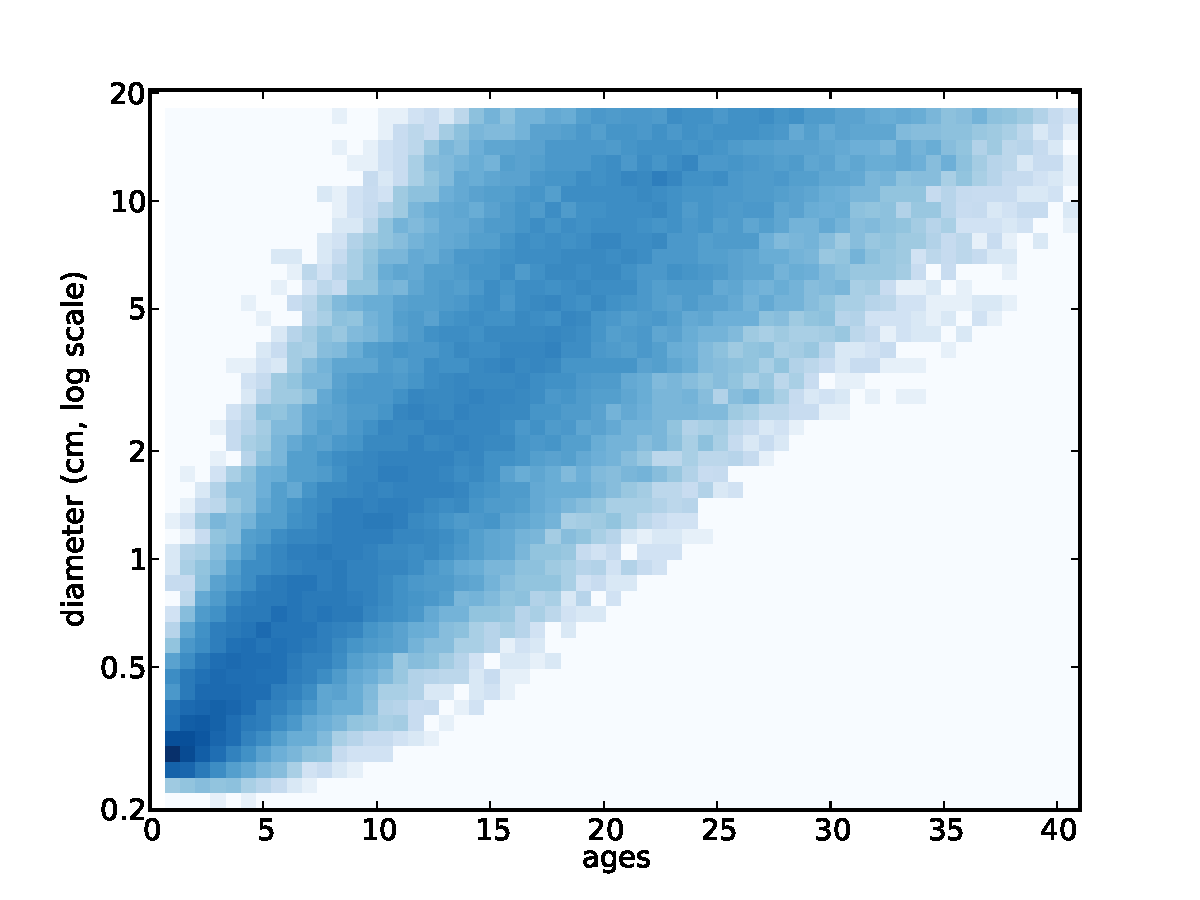
\includegraphics[height=2.5in]{figs/kidney8.pdf}}
\caption{Joint distribution of age and tumor size.}
\label{fig.kidney8}
\end{figure}

Here's how the cache works.  

\begin{code}
class Cache(object):

    def __init__(self):
        self.joint = thinkbayes.Joint()
\end{code}

{\tt joint} is a joint Pmf that records the
frequency of each age-size pair, so it approximates the
joint distribution of age and size.
\index{joint distribution}

At the end of each simulated interval, {\tt ExtendSequence} calls
{\tt Add}:

\begin{code}
# class Cache

    def Add(self, age, seq):
        final = seq[-1]
        cm = Diameter(final)
        bucket = round(CmToBucket(cm))
        self.joint.Incr((age, bucket))
\end{code}

Again, {\tt age} is the age of the tumor, and {\tt seq} is the
sequence of volumes so far.

\begin{figure}
% kidney.py
\centerline{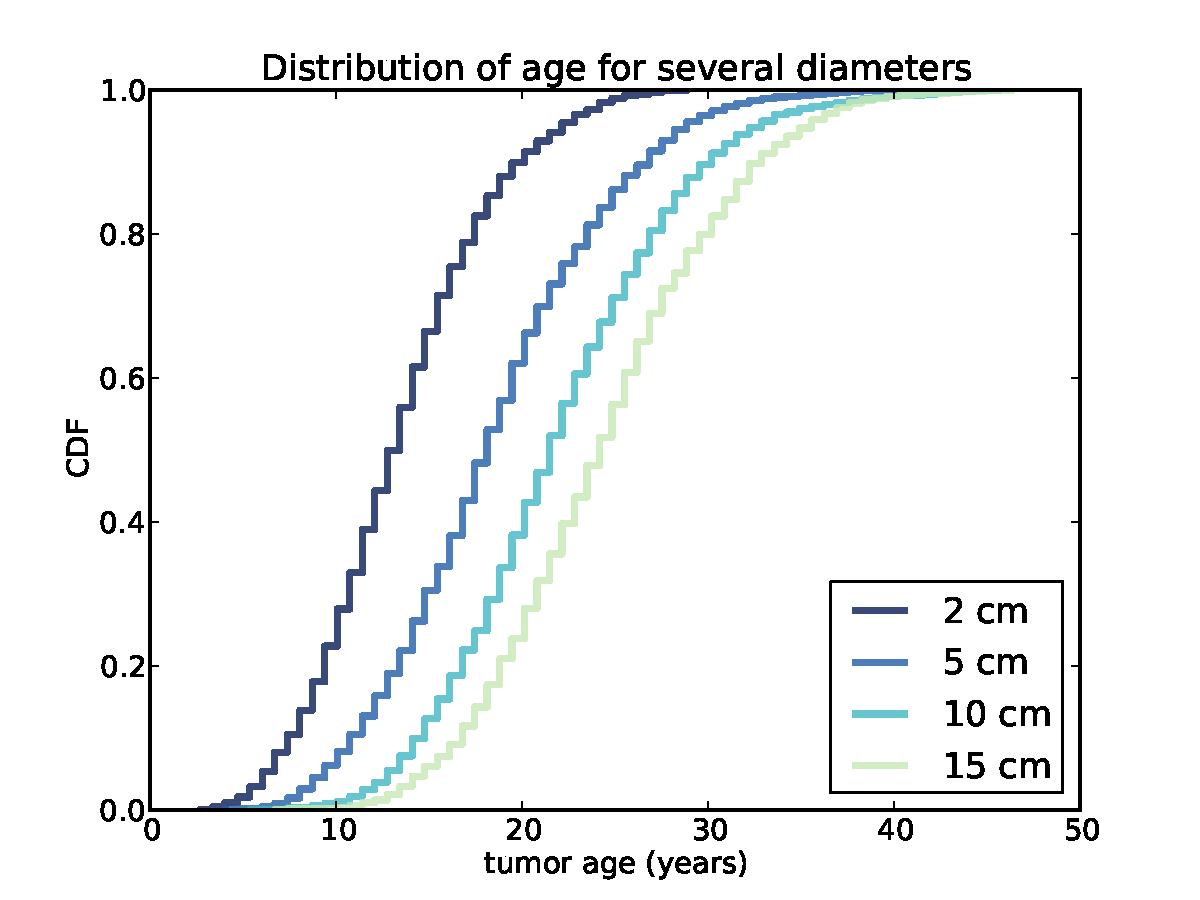
\includegraphics[height=2.5in]{figs/kidney6.pdf}}
\caption{Distributions of age, conditioned on size.}
\label{fig.kidney6}
\end{figure}

Before adding the new data to the joint distribution, we use {\tt
  Diameter} to convert from volume to diameter in centimeters:

\begin{code}
def Diameter(volume, factor=3/math.pi/4, exp=1/3.0):
    return 2 * (factor * volume) ** exp
\end{code}

And
{\tt CmToBucket} to convert from centimeters to a discrete bucket
number:

\begin{code}
def CmToBucket(x, factor=10):
    return factor * math.log(x)
\end{code}

The buckets are equally spaced on a log scale.  Using {\tt factor=10}
yields a reasonable number of buckets; for example,
1 cm maps to bucket 0 and 10 cm maps to bucket 23.
\index{log scale}
\index{bucket}

After running the simulations, we can plot the joint distribution
as a pseudocolor plot, where each cell represents the number of
tumors observed at a given size-age pair.
Figure~\ref{fig.kidney8} shows the joint distribution after 1000
simulations.
\index{pseudocolor plot}



\section{Conditional distributions}

\begin{figure}
% kidney.py
\centerline{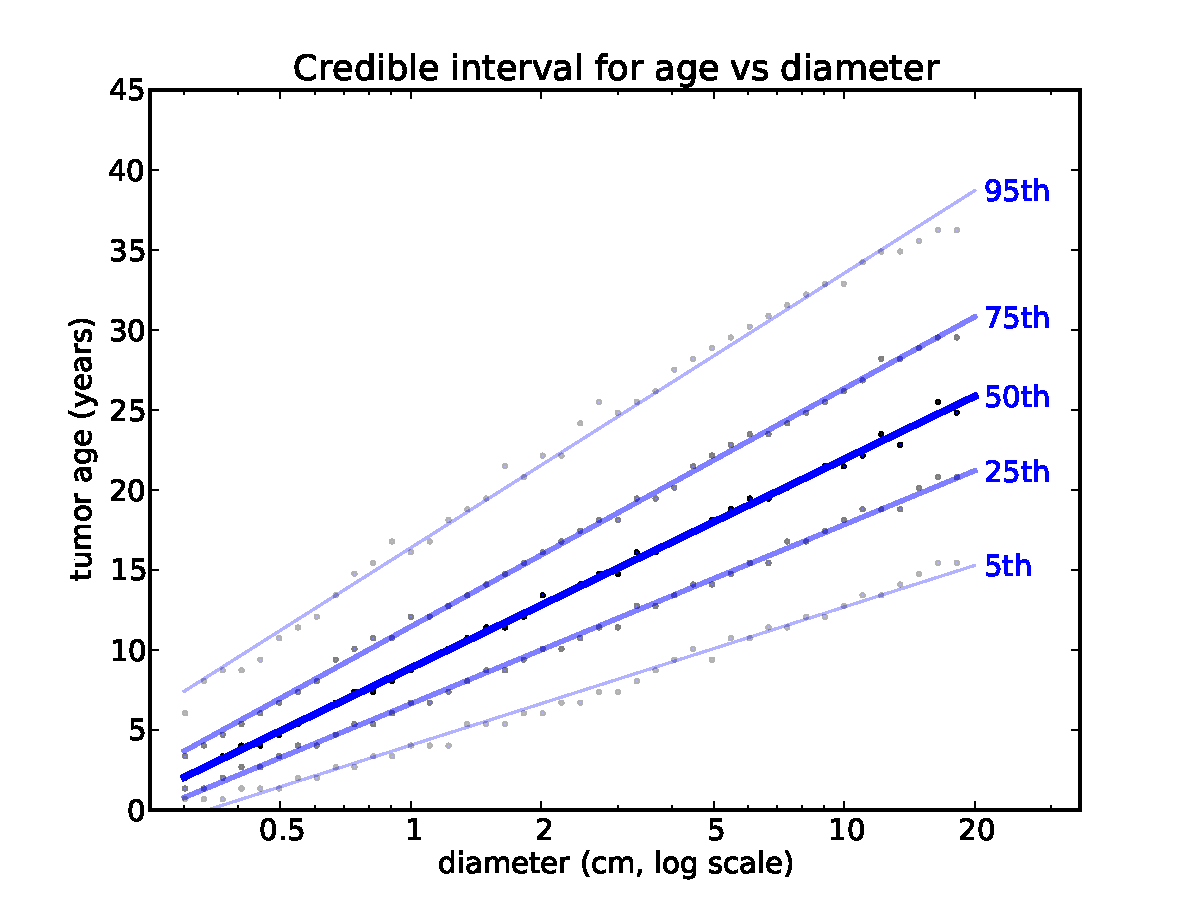
\includegraphics[height=2.5in]{figs/kidney7.pdf}}
\caption{Percentiles of tumor age as a function of size.}
\label{fig.kidney7}
\end{figure}

By taking a vertical slice from the joint distribution, we can get the
distribution of sizes for any given age.  By taking a horizontal
slice, we can get the distribution of ages conditioned on size.
\index{conditional distribution}

Here's the code that reads the joint distribution and builds
the conditional distribution for a given size.
\index{joint distribution}

\begin{code}
# class Cache

    def ConditionalCdf(self, bucket):
        pmf = self.joint.Conditional(0, 1, bucket)
        cdf = pmf.MakeCdf()
        return cdf
\end{code}

\verb"bucket" is the integer bucket number corresponding to
tumor size.  {\tt Joint.Conditional} computes the
PMF of age conditioned on {\tt bucket}.
The result is the CDF of age conditioned on {\tt bucket}.

Figure~\ref{fig.kidney6} shows several of these CDFs, for
a range of sizes.  To summarize these distributions, we can
compute percentiles as a function of size.
\index{percentile}

\begin{code}
    percentiles = [95, 75, 50, 25, 5]

    for bucket in cache.GetBuckets():
        cdf = ConditionalCdf(bucket)      
        ps = [cdf.Percentile(p) for p in percentiles]
\end{code}

Figure~\ref{fig.kidney7} shows these percentiles for each
size bucket.  The data points are computed from the estimated
joint distribution.  In the model, size and time are discrete,
which contributes numerical errors, so I also show a least 
squares fit for each sequence of percentiles.
\index{least squares fit}


\section{Serial Correlation}
\label{serial}

The results so far are based on a number of modeling decisions;
let's review them and consider which ones are the most
likely sources of error:
\index{modeling error}

\begin{itemize}

\item To convert from linear measure to volume, we assume that
  tumors are approximately spherical.  This assumption is probably
  fine for tumors up to a few centimeters, but not for very
  large tumors.
  \index{sphere}

\item The distribution of growth rates in the simulations are based on
  a continuous model we chose to fit the data reported by Zhang et al,
  which is based on 53 patients.  The fit is only approximate and, more
  importantly, a larger sample would yield a
  different distribution.
  \index{growth rate}

\item The growth model does not take into account tumor subtype or
  grade; this assumption is consistent with the conclusion of Zhang et al:
  ``Growth rates in renal tumors of different sizes, subtypes and
  grades represent a wide range and overlap substantially.''
  But with a larger sample, a difference might become apparent.
  \index{tumor type}

\item The distribution of growth rate does not depend on the size of
  the tumor.  This assumption would not be realistic for very
  small and very large tumors, whose growth is limited by blood supply.

  But tumors observed by Zhang et al ranged from 1 to 12 cm, and they
  found no statistically significant relationship between
  size and growth rate.  So if there is a relationship, it is
  likely to be weak, at least in this size range.
  
\item In the simulations, growth rate during each interval is
  independent of previous growth rates.  In reality it is plausible
  that tumors that have grown quickly in the past are more likely
  to grow quickly.  In other words, there is probably
  a serial correlation in growth rate.
  \index{serial correlation}

\end{itemize}

Of these, the first and last seem the most problematic.  I'll
investigate serial correlation first, then come back to
spherical geometry.

To simulate correlated growth, I wrote a generator\footnote{If you are
  not familiar with Python generators, see
  \url{http://wiki.python.org/moin/Generators}.} that yields a
correlated series from a given Cdf.  Here's how the algorithm works:
\index{generator}

\begin{enumerate}

\item Generate correlated values from a Gaussian distribution.
  This is easy to do because we can compute the distribution
  of the next value conditioned on the previous value.
  \index{Gaussian distribution}

\item Transform each value to its cumulative probability using
  the Gaussian CDF.
  \index{cumulative probability}

\item Transform each cumulative probability to the corresponding value
  using the given Cdf.

\end{enumerate}

Here's what that looks like in code:

\begin{code}
def CorrelatedGenerator(cdf, rho):
    x = random.gauss(0, 1)
    yield Transform(x)

    sigma = math.sqrt(1 - rho**2);    
    while True:
        x = random.gauss(x * rho, sigma)
        yield Transform(x)
\end{code}

{\tt cdf} is the desired Cdf; {\tt rho} is the desired correlation.
The values of {\tt x} are Gaussian; {\tt Transform} converts them
to the desired distribution.

The first value of {\tt x} is Gaussian with mean 0 and standard
deviation 1.  For subsequent values, the mean and standard deviation
depend on the previous value.  Given the previous {\tt x}, the mean of the
next value is {\tt x * rho}, and the variance is {\tt 1 - rho**2}.
\index{correlated random value}

{\tt Transform} maps from each
Gaussian value, {\tt x}, to a value from the given Cdf, {\tt y}.

\begin{code}
    def Transform(x):
        p = thinkbayes.GaussianCdf(x)
        y = cdf.Value(p)
        return y
\end{code}

{\tt GaussianCdf} computes the CDF of the standard Gaussian
distribution at {\tt x}, returning a cumulative probability.
{\tt Cdf.Value} maps from a cumulative probability to the
corresponding value in {\tt cdf}.

Depending on the shape of {\tt cdf}, information can
be lost in transformation, so the actual correlation might be
lower than {\tt rho}.  For example, when I generate
10000 values from the distribution of growth rates with
{\tt rho=0.4}, the actual correlation is 0.37.
But since we are guessing at the right correlation anyway,
that's close enough.

Remember that {\tt MakeSequence} takes an iterator as an argument.
That interface allows it to work with different generators:
\index{generator}

\begin{code}
    iterator = UncorrelatedGenerator(cdf)
    seq1 = MakeSequence(iterator)

    iterator = CorrelatedGenerator(cdf, rho)
    seq2 = MakeSequence(iterator)
\end{code}

In this example, {\tt seq1} and {\tt seq2} are
drawn from the same distribution, but the values in {\tt seq1}
are uncorrelated and the values in {\tt seq2} are correlated
with a coefficient of approximately {\tt rho}.
\index{serial correlation}

Now we can see what effect serial correlation has on the results;
the following table shows percentiles of age for a 6 cm tumor,
using the uncorrelated generator and a correlated generator
with target $\rho = 0.4$.
\index{percentile}

\begin{table}
\begin{tabular}{|l|r||r|r|r|r|r|}
\hline
Serial       & Diameter   & \multicolumn{5}{c|}{Percentiles of age} \\
Correlation  & (cm)       & 5th & 25th & 50th & 75th & 95th \\
\hline
0.0 & 6.0 & 10.7  & 15.4  & 19.5  & 23.5  & 30.2 \\
0.4 & 6.0 & 9.4  & 15.4  & 20.8  & 26.2  & 36.9 \\
\hline
\end{tabular}

\caption{Percentiles of tumor age conditioned on size.}
\end{table}

Correlation makes the fastest growing tumors faster and the slowest
slower, so the range of ages is wider.  The difference is modest for
low percentiles, but for the 95th percentile it is more than 6 years.
To compute these percentiles precisely, we would need a better
estimate of the actual serial correlation.

However, this model is sufficient to answer the question
we started with: given a tumor with a linear dimension of
15.5 cm, what is the probability that it formed more than
8 years ago?

Here's the code:

\begin{code}
# class Cache

    def ProbOlder(self, cm, age):
        bucket = CmToBucket(cm)
        cdf = self.ConditionalCdf(bucket)
        p = cdf.Prob(age)
        return 1-p
\end{code}

{\tt cm} is the size of the tumor; {\tt age} is the age threshold
in years.  {\tt ProbOlder} converts size to a bucket number,
gets the Cdf of age conditioned on bucket, and computes the
probability that age exceeds the given value.

With no serial correlation, the probability that a
15.5 cm tumor is older than 8 years is 0.999, or almost certain.
With correlation 0.4, faster-growing tumors are more likely, but
the probability is still 0.995.  Even with correlation 0.8, the
probability is 0.978.

Another likely source of error is the assumption that tumors are
approximately spherical.  For a tumor with linear dimensions 15.5 x 15
cm, this assumption is probably not valid.  If, as seems likely, a
tumor this size
is relatively flat, it might have the same volume as a 6 cm sphere.
With this smaller volume and correlation 0.8, the probability of age
greater than 8 is still 95\%.

So even taking into account modeling errors, it is unlikely that such
a large tumor could have formed less than 8 years prior to the date of
diagnosis.
\index{modeling error}


\section{Discussion}

Well, we got through a whole chapter without using Bayes's theorem or
the {\tt Suite} class that encapsulates Bayesian updates.  What
happened?

One way to think about Bayes's theorem is as an algorithm for
inverting conditional probabilities.  Given \p{B|A}, we can compute
\p{A|B}, provided we know \p{A} and \p{B}.  Of course this algorithm
is only useful if, for some reason, it is easier to compute \p{B|A}
than \p{A|B}.

In this example, it is.  By running simulations, we can estimate the
distribution of size conditioned on age, or \p{size|age}.  But it is
harder to get the distribution of age conditioned on size, or
\p{age|size}.  So this seems like a perfect opportunity to use Bayes's
theorem.

The reason I didn't is computational efficiency.  To estimate
\p{size|age} for any given size, you have to run a lot of simulations.
Along the way, you end up computing \p{size|age} for a lot of sizes.
In fact, you end up computing the entire joint distribution of size
and age, \p{size, age}.
\index{joint distribution}

And once you have the joint distribution, you don't really need
Bayes's theorem, you can extract \p{age|size} by taking slices from
the joint distribution, as demonstrated in {\tt ConditionalCdf}.
\index{conditional distribution}

So we side-stepped Bayes, but he was with us in spirit.


\chapter{A Hierarchical Model}
\label{hierarchical}


\section{The Geiger counter problem}

I got the idea for the following problem from Tom Campbell-Ricketts,
author of the Maximum Entropy blog at
\url{http://maximum-entropy-blog.blogspot.com}.  And he got the idea
from E.~T.~Jaynes, author of the classic {\em Probability Theory: The
  Logic of Science}:
\index{Jaynes, E.~T.}
\index{Campbell-Ricketts, Tom}
\index{Geiger counter problem}

\begin{quote}
Suppose that a radioactive source emits particles toward
a Geiger counter at an average rate of $r$ particles per second,
but the counter only registers a fraction, $f$, of the particles
that hit it.  If $f$ is 10\% and
the counter registers 15 particles in a one second
interval, what is the posterior distribution of $n$, the actual
number of particles that hit the counter, and $r$, the average
rate particles are emitted?
\end{quote}

To get started on a problem like this, think about the chain of
causation that starts with the parameters of the system and ends
with the observed data:
\index{causation}

\begin{enumerate}

\item The source emits particles at an average rate, $r$.

\item During any given second, the source emits $n$ particles
toward the counter.

\item Out of those $n$ particles, some number, $k$, get counted.

\end{enumerate}

The probability that an atom decays is the same at any point in time,
so radioactive decay is well modeled by a Poisson process.  Given $r$,
the distribution of $n$ is Poisson distribution with parameter $r$.
\index{radioactive decay}
\index{Poisson process}

And if we assume that the probability of detection for each particle
is independent of the others, the distribution of $k$ is the binomial
distribution with parameters $n$ and $f$.
\index{binomial distribution}

Given the parameters of the system, we can find the distribution of
the data.  So we can solve what is called the {\bf forward problem}.
\index{forward problem}

Now we want to go the other way: given the data, we
want the distribution of the parameters.  This is called
the {\bf inverse problem}.  And if you can solve the forward
problem, you can use Bayesian methods to solve the inverse problem.
\index{inverse problem}


\section{Start simple}

\begin{figure}
% jaynes.py
\centerline{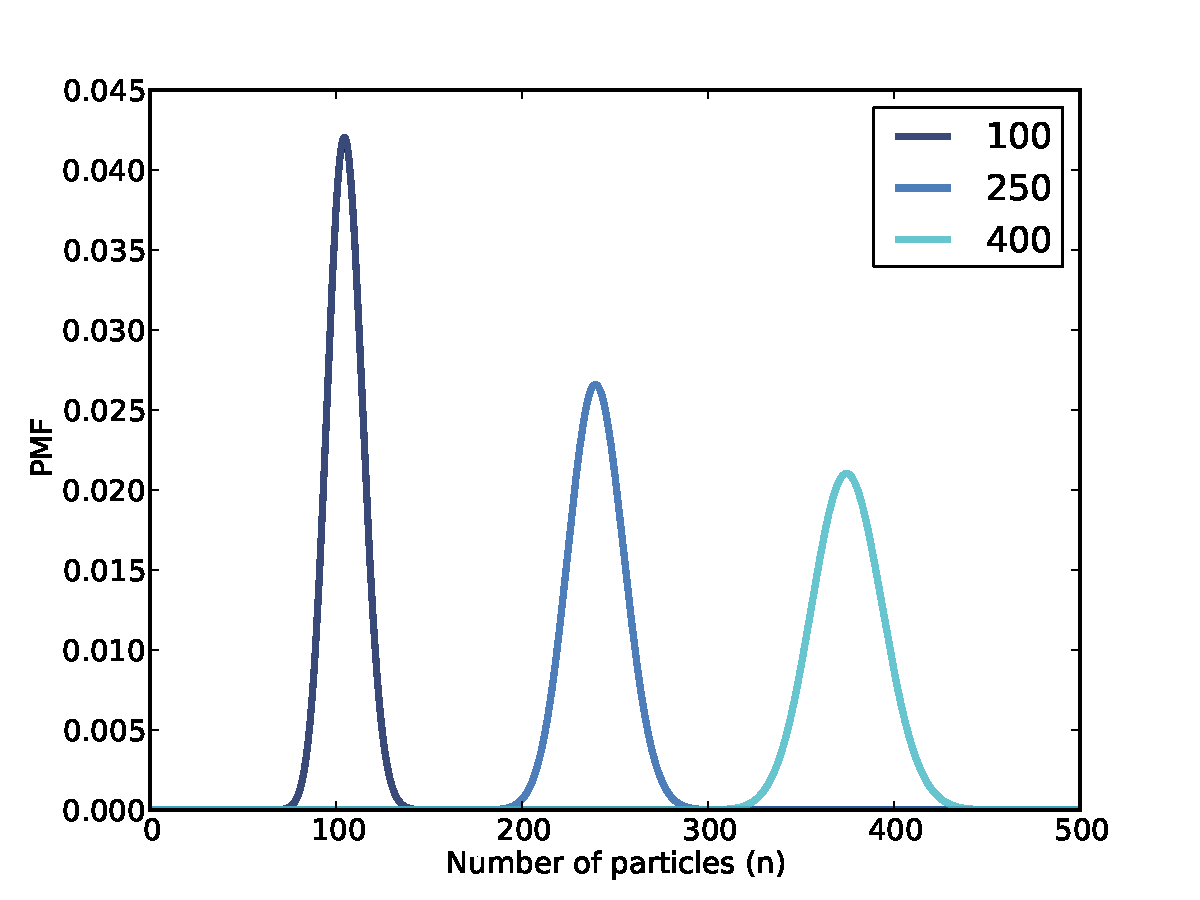
\includegraphics[height=2.5in]{figs/jaynes1.pdf}}
\caption{Posterior distribution of $n$ for three values of $r$.}
\label{fig.jaynes1}
\end{figure}

Let's start with a simple version of the problem where we know
the value of $r$.  We are given the value of $f$, so all we
have to do is estimate $n$.

I define a Suite called {\tt Detector} that models the behavior
of the detector and estimates $n$.

\begin{code}
class Detector(thinkbayes.Suite):

    def __init__(self, r, f, high=500, step=1):
        pmf = thinkbayes.MakePoissonPmf(r, high, step=step)
        thinkbayes.Suite.__init__(self, pmf, name=r)
        self.r = r
        self.f = f
\end{code}

If the average emission rate is $r$ particles per second, the
distribution of $n$ is Poisson with parameter $r$.
{\tt high} and {\tt step} determine the upper bound for $n$
and the step size between hypothetical values.
\index{Poisson distribution}

Now we need a likelihood function:
\index{likelihood}

\begin{code}
# class Detector

    def Likelihood(self, data, hypo):
        k = data
        n = hypo
        p = self.f

        return thinkbayes.EvalBinomialPmf(k, n, p)
\end{code}

{\tt data} is the number of particles detected, and {\tt hypo} is
the hypothetical number of particles emitted, $n$.

If there are actually $n$ particles, and the probability of detecting
any one of them is $f$, the probability of detecting $k$ particles is
given by the binomial distribution.
\index{binomial distribution}

That's it for the Detector.  We can try it out for a range
of values of $r$:

\begin{code}
    f = 0.1
    k = 15

    for r in [100, 250, 400]:
        suite = Detector(r, f, step=1)
        suite.Update(k)
        print suite.MaximumLikelihood()
\end{code}

Figure~\ref{fig.jaynes1} shows the posterior distribution of $n$ for
several given values of $r$.


\section{Make it hierarchical}

In the previous section, we assume $r$ is known.  Now let's
relax that assumption.  I define another Suite, called {\tt Emitter},
that models the behavior of the emitter and estimates $r$:

\begin{code}
class Emitter(thinkbayes.Suite):

    def __init__(self, rs, f=0.1):
        detectors = [Detector(r, f) for r in rs]
        thinkbayes.Suite.__init__(self, detectors)
\end{code}

{\tt rs} is a sequence of hypothetical value for $r$.  {\tt detectors}
is a sequence of Detector objects, one for each value of $r$.  The
values in the Suite are Detectors, so Emitter is a {\bf meta-Suite};
that is, a Suite that contains other Suites as values.
\index{meta-Suite}

To update the Emitter, we have to compute the likelihood of the data
under each hypothetical value of $r$.  But each value of $r$ is
represented by a Detector that contains a range of values for $n$.

To compute the likelihood of the data for a given Detector, we loop
through the values of $n$ and add up the total probability of $k$.
That's what {\tt SuiteLikelihood} does:

\begin{code}
# class Detector

    def SuiteLikelihood(self, data):
        total = 0
        for hypo, prob in self.Items():
            like = self.Likelihood(data, hypo)
            total += prob * like
        return total
\end{code}

Now we can write the Likelihood function for the Emitter:

\begin{code}
# class Emitter

    def Likelihood(self, data, hypo):
        detector = hypo
        like = detector.SuiteLikelihood(data)
        return like
\end{code}

Each {\tt hypo} is a Detector, so we can invoke
{\tt SuiteLikelihood} to get the likelihood of the data under
the hypothesis.

After we update the Emitter, we have to update each of the
Detectors, too.  

\begin{code}
# class Emitter

    def Update(self, data):
        thinkbayes.Suite.Update(self, data)
        
        for detector in self.Values():
            detector.Update()
\end{code}

A model like this, with multiple levels of Suites, is called {\bf
  hierarchical}.  \index{hierarchical model}


\section{A little optimization}

You might recognize {\tt SuiteLikelihood}; we saw it
in Section~\ref{suitelike}.  At the time, I pointed out that
we didn't really need it, because the total probability
computed by {\tt SuiteLikelihood} is exactly the normalizing
constant computed and returned by {\tt Update}.
\index{normalizing constant}
 
So instead of updating the Emitter and then updating the
Detectors, we can do both steps at the same time, using
the result from {\tt Detector.Update} as the likelihood
of Emitter.

Here's the streamlined version of {\tt Emitter.Likelihood}:

\begin{code}
# class Emitter

    def Likelihood(self, data, hypo):
        return hypo.Update(data)
\end{code}

And with this version of {\tt Likelihood} we can use the
default version of {\tt Update}.  So this version has fewer
lines of code, and it runs faster because it does not compute
the normalizing constant twice.
\index{optimization}


\section{Extracting the posteriors}

\begin{figure}
% jaynes.py
\centerline{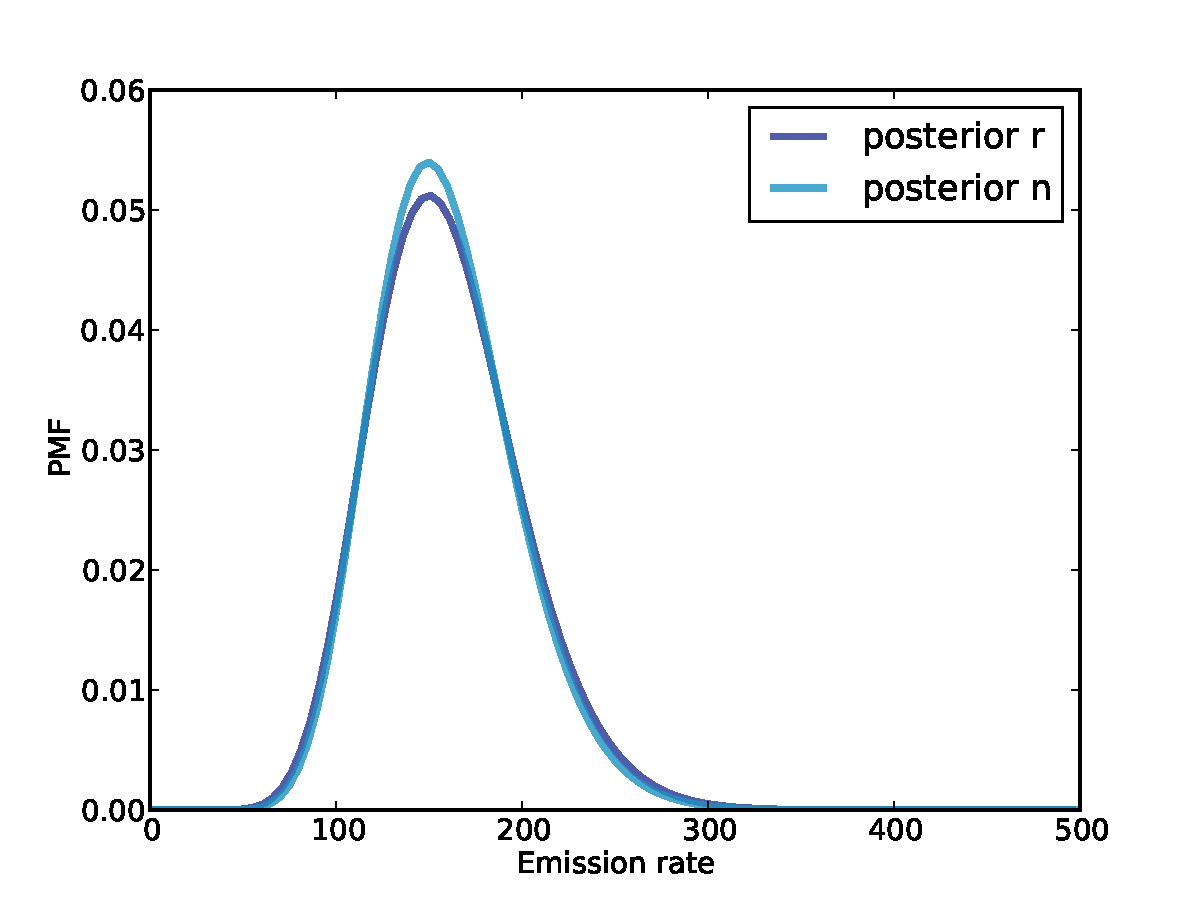
\includegraphics[height=2.5in]{figs/jaynes2.pdf}}
\caption{Posterior distributions of $n$ and $r$.}
\label{fig.jaynes2}
\end{figure}

After we update the Emitter, we can get the posterior distribution
of $r$ by looping through the Detectors and their probabilities:

\begin{code}
# class Emitter

    def DistOfR(self):
        items = [(detector.r, prob) for detector, prob in self.Items()]
        return thinkbayes.MakePmfFromItems(items)
\end{code}

{\tt items} is a list of values of $r$ and their probabilities.
The result is the Pmf of $r$.

To get the posterior distribution of $n$, we have to compute
the mixture of the Detectors.  We can use 
{\tt thinkbayes.MakeMixture}, which takes a meta-Pmf that maps
from each distribution to its probability.  And that's exactly
what the Emitter is:

\begin{code}
# class Emitter

    def DistOfN(self):
        return thinkbayes.MakeMixture(self)
\end{code}

Figure~\ref{fig.jaynes2} shows the results.  Not surprisingly, the
most likely value for $n$ is 150.  Given $f$ and $n$, the expected
count is $k = f n$, so given $f$ and $k$, the expected value of $n$ is
$k / f$, which is 150.

And if 150 particles are emitted in one second, the most likely value
of $r$ is 150 particles per second.  So the posterior distribution of
$r$ is also centered on 150.

The posterior distributions of $r$ and $n$ are similar;
the only difference is that we are slightly less certain about $n$.
In general, we can be more certain about the long-range emission rate,
$r$, than about the number of particles emitted in any particular second,
$n$.

You can download the code in this chapter from
\url{http://thinkbayes.com/jaynes.py}.  For more information see
Section~\ref{download}.


\section{Discussion}

The Geiger counter problem demonstrates the connection between
causation and hierarchical modeling.  In the example, the
emission rate $r$ has a causal effect on the number of particles,
$n$, which has a causal effect on the particle count, $k$.
\index{Geiger counter problem}
\index{causation}

The hierarchical model reflects the structure of the
system, with causes at the top and effects at the bottom.
\index{hierarchical model}

\begin{enumerate}

\item At the top level, we start with a range of hypothetical
values for $r$.

\item For each value of $r$, we have a range of values for $n$,
and the prior distribution of $n$ depends on $r$.

\item When we update the model, we go bottom-up.  We compute
a posterior distribution of $n$ for each value of $r$, then
compute the posterior distribution of $r$.

\end{enumerate}

So causal information flows down the hierarchy, and inference flows
up.


\section{Exercises}

\begin{exercise}
This exercise is also inspired by an example in Jaynes, {\em
Probability Theory}.

Suppose you buy a mosquito trap that is supposed to reduce the
population of mosquitoes near your house.  Each
week, you empty the trap and count the number of mosquitoes
captured.  After the first week, you count 30 mosquitoes.
After the second week, you count 20 mosquitoes.  Estimate the
percentage change in the number of mosquitoes in your yard.

To answer this question, you have to make some modeling
decisions.  Here are some suggestions:

\begin{itemize}

\item Suppose that each week a large number of mosquitoes, $N$, is bred
in a wetland near your home.

\item During the week, some fraction of
them, $f_1$, wander into your yard, and of those some fraction, $f_2$,
are caught in the trap.

\item Your solution should take into account your prior belief
about how much $N$ is likely to change from one week to the next.
You can do that by adding a level to the hierarchy to
model the percent change in $N$.

\end{itemize}

\end{exercise}


\chapter{Dealing with Dimensions}
\label{species}

\section{Belly button bacteria}

Belly Button Biodiversity 2.0 (BBB2) is a nation-wide citizen
science project with the goal of identifying bacterial species that
can be found in human navels (\url{http://bbdata.yourwildlife.org}).
The project might seem whimsical, but it is part of an increasing
interest in the human microbiome, the set of microorganisms that live
on human skin and parts of the body.
\index{biodiversity}
\index{belly button}
\index{bacteria}
\index{microbiome}

In their pilot study, BBB2 researchers collected swabs from the navels
of 60 volunteers, used multiplex pyrosequencing to extract and sequence
fragments of 16S rDNA, then identified the species or genus the
fragments came from.  Each identified fragment is called a ``read.''
\index{navel}
\index{rDNA}
\index{pyrosequencing}

We can use these data to answer several related questions:

\begin{itemize}

\item Based on the number of species observed, can we estimate
  the total number of species in the environment?
\index{species}

\item Can we estimate the prevalence of each species; that is, the
  fraction of the total population belonging to each species?
\index{prevalence}

\item If we are planning to collect additional samples, can we predict
  how many new species we are likely to discover?

\item How many additional reads are needed to increase the
  fraction of observed species to a given threshold?

\end{itemize}

These questions make up what is called the {\bf Unseen Species problem}.
\index{Unseen Species problem}


\section{Lions and tigers and bears}

I'll start with a simplified version of the problem where we know that
there are exactly three species.  Let's call them lions, tigers and
bears.  Suppose we visit a wild animal preserve and see 3 lions, 2
tigers and one bear.
\index{lions and tigers and bears}

If we have an equal chance of observing any animal in the preserve,
the number of each species we see is governed by the multinomial
distribution.  If the prevalence of lions and tigers and bears is
\verb"p_lion" and \verb"p_tiger" and \verb"p_bear", the likelihood of
seeing 3 lions, 2 tigers and one bear is proportional to
\index{multinomial distribution}

\begin{code}
p_lion**3 * p_tiger**2 * p_bear**1
\end{code}

An approach that is tempting, but not correct, is to use beta
distributions, as in Section~\ref{beta}, to describe the prevalence of
each species separately.  For example, we saw 3 lions and 3 non-lions;
if we think of that as 3 ``heads'' and 3 ``tails,'' then the posterior
distribution of \verb"p_lion" is:
\index{beta distribution}

\begin{code}
    beta = thinkbayes.Beta()
    beta.Update((3, 3))
    print beta.MaximumLikelihood()
\end{code}

The maximum likelihood estimate for \verb"p_lion" is the observed
rate, 50\%.  Similarly the MLEs for \verb"p_tiger" and \verb"p_bear"
are 33\% and 17\%.
\index{maximum likelihood}

But there are two problems:

\begin{enumerate}

\item We have implicitly used a prior for each species that is uniform
  from 0 to 1, but since we know that there are three species, that
  prior is not correct.  The right prior should have a mean of 1/3,
  and there should be zero likelihood that any species has a
  prevalence of 100\%.

\item The distributions for each species are not independent, because
  the prevalences have to add up to 1.  To capture this dependence, we
  need a joint distribution for the three prevalences.
\index{independence}
\index{joint distribution}

\end{enumerate}

We can use a Dirichlet distribution to solve both of these problems
(see \url{http://en.wikipedia.org/wiki/Dirichlet_distribution}).  In
the same way we used the beta distribution to describe the
distribution of bias for a coin, we can use a Dirichlet
distribution to describe the joint distribution of \verb"p_lion",
\verb"p_tiger" and \verb"p_bear".
\index{beta distribution}
\index{Dirichlet distribution}

The Dirichlet distribution is the multi-dimensional generalization
of the beta distribution.  Instead of two possible outcomes, like
heads and tails, the Dirichlet distribution handles any number of
outcomes: in this example, three species.

If there are {\tt n} outcomes, the Dirichlet distribution is
described by {\tt n} parameters, written $\alpha_1$ through $\alpha_n$.

Here's the definition, from {\tt thinkbayes.py}, of a class that
represents a Dirichlet distribution:
\index{numpy}

\begin{code}
class Dirichlet(object):

    def __init__(self, n):
        self.n = n
        self.params = numpy.ones(n, dtype=numpy.int)
\end{code}

{\tt n} is the number of dimensions; initially the parameters
are all 1.  I use a {\tt numpy} array to store the parameters
so I can take advantage of array operations.

Given a Dirichlet distribution, the marginal distribution
for each prevalence is a beta distribution, which we can
compute like this:

\begin{code}
    def MarginalBeta(self, i):
        alpha0 = self.params.sum()
        alpha = self.params[i]
        return Beta(alpha, alpha0-alpha)
\end{code}

{\tt i} is the index of the marginal distribution we want.
{\tt alpha0} is the sum of the parameters; {\tt alpha} is the
parameter for the given species.
\index{marginal distribution}

In the example, the prior marginal distribution for each species
is {\tt Beta(1, 2)}.  We can compute the prior means like
this:

\begin{code}
    dirichlet = thinkbayes.Dirichlet(3)
    for i in range(3):
        beta = dirichlet.MarginalBeta(i)
        print beta.Mean()
\end{code}

As expected, the prior mean prevalence for each species is 1/3.

To update the Dirichlet distribution, we add the
observations to the parameters like this:

\begin{code}
    def Update(self, data):
        m = len(data)
        self.params[:m] += data
\end{code}

Here {\tt data} is a sequence of counts in the same order as {\tt
  params}, so in this example, it should be the number of lions,
tigers and bears.

{\tt data} can be shorter than {\tt params}; in that
case there are some species that have not been
observed.

Here's code that updates {\tt dirichlet} with the observed data and
computes the posterior marginal distributions.

\begin{code}
    data = [3, 2, 1]
    dirichlet.Update(data)

    for i in range(3):
        beta = dirichlet.MarginalBeta(i)
        pmf = beta.MakePmf()
        print i, pmf.Mean()
\end{code}

\begin{figure}
% species.py
\centerline{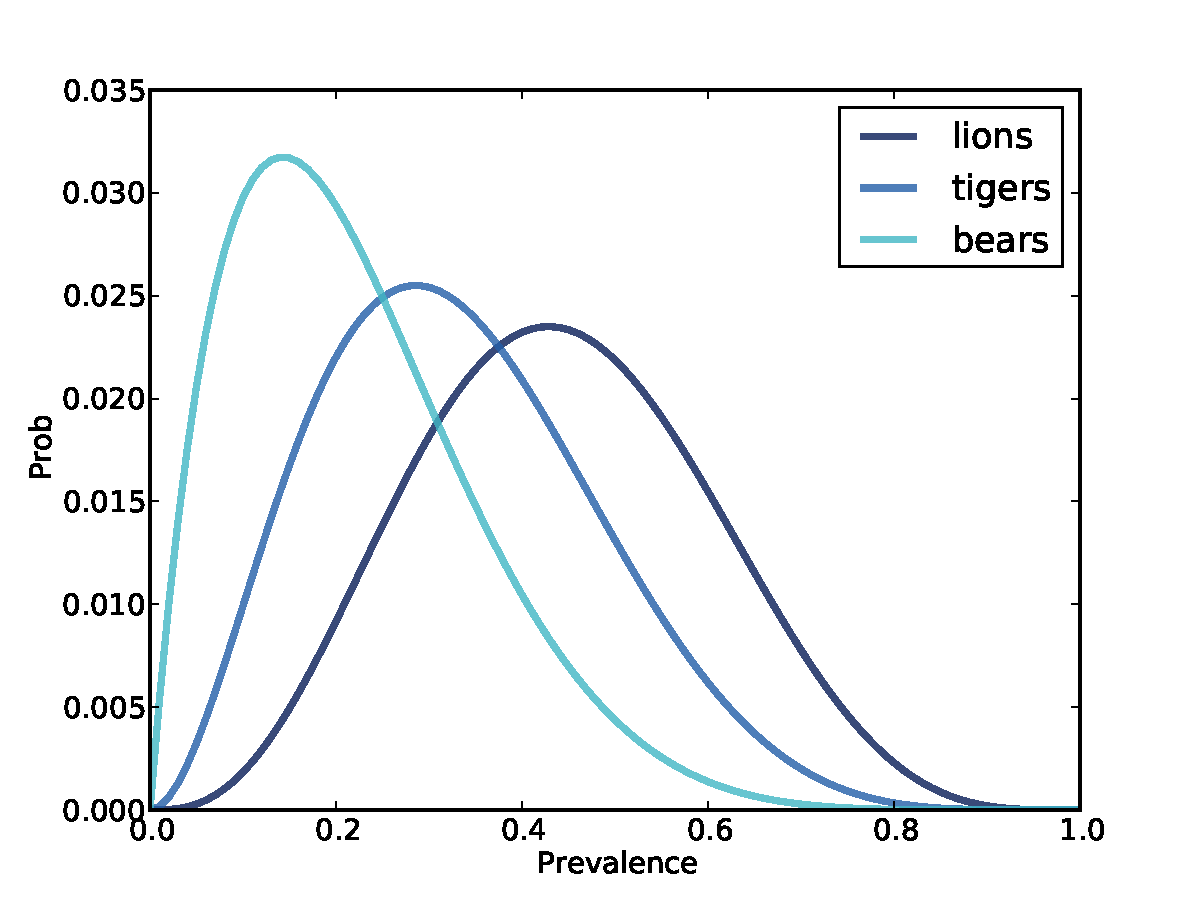
\includegraphics[height=2.5in]{figs/species1.pdf}}
\caption{Distribution of prevalences for three species.}
\label{fig.species1}
\end{figure}

Figure~\ref{fig.species1} shows the results.  The posterior
mean prevalences are 44\%, 33\%, and 22\%.


\section{The hierarchical version}

We have solved a simplified version of the problem: if we
know how many species there are, we can estimate the prevalence
of each.
\index{prevalence}

Now let's get back to the original problem, estimating the total
number of species.  To solve this problem I'll define a meta-Suite,
which is a Suite that contains other Suites as hypotheses.  In this
case, the top-level Suite contains hypotheses about the number of
species; the bottom level contains hypotheses about prevalences.
\index{hierarchical model}
\index{meta-Suite}

Here's the class definition:

\begin{code}
class Species(thinkbayes.Suite):

    def __init__(self, ns):
        hypos = [thinkbayes.Dirichlet(n) for n in ns]
        thinkbayes.Suite.__init__(self, hypos)
\end{code}

\verb"__init__" takes a list of possible values for {\tt n} and
makes a list of Dirichlet objects.

Here's the code that creates the top-level suite:

\begin{code}
    ns = range(3, 30)
    suite = Species(ns)
\end{code}

{\tt ns} is the list of possible values for {\tt n}.  We have seen 3
species, so there have to be at least that many.  I chose an upper
bound that seems reasonable, but we will check later that the
probability of exceeding this bound is low.  And at least initially
we assume that any value in this range is equally likely.

To update a hierarchical model, you have to update all levels.
Usually you have to update the bottom
level first and work up, but in this case we can
update the top level first:

\begin{code}
#class Species

    def Update(self, data):
        thinkbayes.Suite.Update(self, data)
        for hypo in self.Values():
            hypo.Update(data)
\end{code}

{\tt Species.Update} invokes {\tt Update} in the parent class,
then loops through the sub-hypotheses and updates them.

Now all we need is a likelihood function:

\begin{code}
# class Species

    def Likelihood(self, data, hypo):
        dirichlet = hypo
        like = 0
        for i in range(1000):
            like += dirichlet.Likelihood(data)

        return like
\end{code}

{\tt data} is a sequence of
observed counts; {\tt hypo} is a Dirichlet object.
{\tt Species.Likelihood} calls
{\tt Dirichlet.Likelihood} 1000 times and returns the total.

Why call it 1000 times?  Because {\tt
  Dirichlet.Likelihood} doesn't actually compute the likelihood of the
data under the whole Dirichlet distribution.  Instead, it draws one
sample from the hypothetical distribution and computes the likelihood
of the data under the sampled set of prevalences.

Here's what it looks like:

\begin{code}
# class Dirichlet

    def Likelihood(self, data):
        m = len(data)
        if self.n < m:
            return 0

        x = data
        p = self.Random()
        q = p[:m]**x
        return q.prod()
\end{code}

The length of {\tt data} is the number of species observed.  If
we see more species than we thought existed, the likelihood is 0.

\index{multinomial distribution}
Otherwise we select a random set of prevalences, {\tt p}, and
compute the multinomial PMF, which is
%
\[ c_x  p_1^{x_1} \cdots p_n^{x_n} \]
%
$p_i$ is the prevalence of the $i$th species, and $x_i$ is the
observed number.  The first term, $c_x$, is the multinomial
coefficient; I leave it out of the computation because it is
a multiplicative factor that depends only
on the data, not the hypothesis, so it gets normalized away
(see \url{http://en.wikipedia.org/wiki/Multinomial_distribution}).
\index{multinomial coefficient}

{\tt m} is the number of observed species.
We only need the first {\tt m} elements of {\tt p};
for the others, $x_i$ is 0, so
$p_i^{x_i}$ is 1, and we can leave them out of the product.


\section{Random sampling}
\label{randomdir}

There are two ways to generate a random sample from a Dirichlet
distribution.  One is to use the marginal beta distributions, but in
that case you have to select one at a time and scale the rest so they
add up to 1 (see
\url{http://en.wikipedia.org/wiki/Dirichlet_distribution#Random_number_generation}).
\index{random sample}

A less obvious, but faster, way is to select values from {\tt n} gamma
distributions, then normalize by dividing through by the total. 
Here's the code:
\index{numpy}
\index{gamma distribution}

\begin{code}
# class Dirichlet

    def Random(self):
        p = numpy.random.gamma(self.params)
        return p / p.sum()
\end{code}

Now we're ready to look at some results.  Here is the code that extracts
the posterior distribution of {\tt n}:

\begin{code}
    def DistOfN(self):
        pmf = thinkbayes.Pmf()
        for hypo, prob in self.Items():
            pmf.Set(hypo.n, prob)
        return pmf
\end{code}

{\tt DistOfN} iterates
through the top-level hypotheses and accumulates the probability
of each {\tt n}.

\begin{figure}
% species.py
\centerline{\includegraphics[height=2.5in]{figs/species2.pdf}}
\caption{Posterior distribution of {\tt n}.}
\label{fig.species2}
\end{figure}

Figure~\ref{fig.species2} shows the result.  The most likely value is 4.
Values from 3 to 7 are reasonably likely; after that the probabilities
drop off quickly.  The probability that there are 29 species is
low enough to be negligible; if we chose a higher bound, 
we would get nearly the same result.

Remember that this result is based on a uniform prior for {\tt n}.  If
we have background information about the number of species in the
environment, we might choose a different prior.  \index{uniform
  distribution}


\section{Optimization}

I have to admit that I am proud of this example.  The Unseen Species
problem is not easy, and I think this solution is simple and clear,
and takes surprisingly few lines of code (about 50 so far).

The only problem is that it is slow.  It's good enough for the example
with only 3 observed species, but not good enough for the belly button
data, with more than 100 species in some samples.

The next few sections present a series of optimizations we need to
make this solution scale.  Before we get into the details, here's
a road map.
\index{optimization}

\begin{itemize}

\item The first step is to recognize that if we update the Dirichlet
  distributions with the same data, the first {\tt m} parameters are
  the same for all of them.  The only difference is the number of
  hypothetical unseen species.  So we don't really need {\tt n}
  Dirichlet objects; we can store the parameters in the top level of
  the hierarchy.  {\tt Species2} implements this optimization.

\item {\tt Species2} also uses the same set of random values for all
  of the hypotheses.  This saves time generating random values, but it
  has a second benefit that turns out to be more important: by giving
  all hypotheses the same selection from the sample space, we make
  the comparison between the hypotheses more fair, so it takes
  fewer iterations to converge.

\item Even with these changes there is a major performance problem.
  As the number of observed species increases, the array of random
  prevalences gets bigger, and the chance of choosing one that is
  approximately right becomes small.  So the vast majority of
  iterations yield small likelihoods that don't contribute much to the
  total, and don't discriminate between hypotheses.

  The solution is to do the updates one species at a time.  {\tt
  Species4} is a simple implementation of this strategy using
  Dirichlet objects to represent the sub-hypotheses.

\item Finally, {\tt Species5} combines the sub-hypotheses into the top
  level and uses {\tt numpy} array operations to speed things up.
\index{numpy}

\end{itemize}

If you are not interested in the details, feel free to skip to
Section~\ref{belly} where we look at results from the belly
button data.


\section{Collapsing the hierarchy}
\label{collapsing}

All of the bottom-level Dirichlet distributions are updated
with the same data, so the first {\tt m} parameters are the same for
all of them.  
We can eliminate them and merge the parameters into
the top-level suite.  {\tt Species2} implements this optimization:
\index{numpy}

\begin{code}
class Species2(object):
    
    def __init__(self, ns):
        self.ns = ns
        self.probs = numpy.ones(len(ns), dtype=numpy.double)
        self.params = numpy.ones(self.high, dtype=numpy.int)
\end{code}

{\tt ns} is the list of hypothetical values for {\tt n};
{\tt probs} is the list of corresponding probabilities.  And
{\tt params} is the sequence of Dirichlet parameters, initially
all 1.

{\tt Species2.Update} updates both levels of
the hierarchy: first the probability for each value of {\tt n},
then the Dirichlet parameters:
\index{numpy}

\begin{code}
# class Species2

    def Update(self, data):
        like = numpy.zeros(len(self.ns), dtype=numpy.double)
        for i in range(1000):
            like += self.SampleLikelihood(data)

        self.probs *= like
        self.probs /= self.probs.sum()

        m = len(data)
        self.params[:m] += data
\end{code}

{\tt SampleLikelihood} returns an array of likelihoods, one for each
value of {\tt n}.  {\tt like} accumulates the total likelihood for
1000 samples.  {\tt self.probs} is multiplied by the total likelihood,
then normalized.  The last two lines, which update the parameters,
are the same as in {\tt Dirichlet.Update}.

Now let's look at {\tt SampleLikelihood}.  There are two
opportunities for optimization here:

\begin{itemize}

\item When the hypothetical number of species, {\tt n},
exceeds the observed number, {\tt m}, we only need the first {\tt m}
terms of the multinomial PMF; the rest are 1.

\item If the number of species is large, the likelihood of the data
  might be too small for floating-point (see ~\ref{underflow}).  So it
  is safer to compute log-likelihoods.
  \index{log-likelihood} \index{underflow}

\end{itemize}

\index{multinomial distribution}
Again, the multinomial PMF is
%
\[ c_x p_1^{x_1} \cdots p_n^{x_n} \]
%
So the log-likelihood is
%
\[ \log c_x + x_1 \log p_1 + \cdots + x_n \log p_n \]
%
which is fast and easy to compute.  Again, $c_x$
it is the same for all hypotheses, so we can drop it.
Here's the code:
\index{numpy}

\begin{code}
# class Species2

    def SampleLikelihood(self, data):
        gammas = numpy.random.gamma(self.params)

        m = len(data)
        row = gammas[:m]
        col = numpy.cumsum(gammas)

        log_likes = []
        for n in self.ns:
            ps = row / col[n-1]
            terms = data * numpy.log(ps)
            log_like = terms.sum()
            log_likes.append(log_like)

        log_likes -= numpy.max(log_likes)
        likes = numpy.exp(log_likes)

        coefs = [thinkbayes.BinomialCoef(n, m) for n in self.ns]
        likes *= coefs

        return likes
\end{code}

{\tt gammas} is an array of values from a gamma distribution; its
length is the largest hypothetical value of {\tt n}.  {\tt row} is
just the first {\tt m} elements of {\tt gammas}; since these are the
only elements that depend on the data, they are the only ones we need.
\index{gamma distribution}

For each value of {\tt n} we need to divide {\tt row} by the
total of the first {\tt n} values from {\tt gamma}.  {\tt cumsum}
computes these cumulative sums and stores them in {\tt col}.
\index{cumulative sum}

The loop iterates through the values of {\tt n} and accumulates
a list of log-likelihoods.
\index{log-likelihood}

Inside the loop, {\tt ps} contains the row of probabilities, normalized
with the appropriate cumulative sum.  {\tt terms} contains the
terms of the summation, $x_i \log p_i$, and \verb"log_like" contains
their sum.

After the loop, we want to convert the log-likelihoods to linear
likelihoods, but first it's a good idea to shift them so the largest
log-likelihood is 0; that way the linear likelihoods are not too
small (see ~\ref{underflow}).

Finally, before we return the likelihood, we have to apply a correction
factor, which is the number of ways we could have observed these {\tt m}
species, if the total number of species is {\tt n}.  
{\tt BinomialCoefficient} computes ``n choose m'', which is written
$\binom{n}{m}$. 
\index{binomial coefficient}

As often happens, the optimized version is less readable and more
error-prone than the original.  But that's one reason I think it is
a good idea to start with the simple version; we can use it for
regression testing.  I plotted results from both versions and confirmed
that they are approximately equal, and that they converge as the
number of iterations increases.
\index{regression testing}


\section{One more problem}

There's more we could do to optimize this code, but there's another
problem we need to fix first.  As the number of observed
species increases, this version gets noisier and takes more
iterations to converge on a good answer.

The problem is that if the prevalences we choose from the Dirichlet
distribution, the {\tt ps}, are not at least approximately right,
the likelihood of the observed data is close to zero and almost
equally bad for all values of {\tt n}.  So most iterations don't
provide any useful contribution to the total likelihood.  And as the
number of observed species, {\tt m}, gets large, the probability of
choosing {\tt ps} with non-negligible likelihood gets small.  Really
small.

Fortunately, there is a solution.  Remember that if you observe
a set of data, you can update the prior distribution with the
entire dataset, or you can break it up into a series of updates
with subsets of the data, and the result is the same either way.

For this example, the key is to perform the updates one species at
a time.  That way when we generate a random set of {\tt ps}, only
one of them affects the computed likelihood, so the chance of choosing
a good one is much better.

Here's a new version that updates one species at a time:
\index{numpy}

\begin{code}
class Species4(Species):

    def Update(self, data):
        m = len(data)

        for i in range(m):
            one = numpy.zeros(i+1)
            one[i] = data[i]            
            Species.Update(self, one)
\end{code}

This version inherits \verb"__init__" from {\tt Species}, so it
represents the hypotheses as a list of Dirichlet objects (unlike
{\tt Species2}).

{\tt Update} loops through the observed species and makes an
array, {\tt one}, with all zeros and one species count.  Then
it calls {\tt Update} in the parent class, which computes
the likelihoods and updates the sub-hypotheses.

So in the running example, we do three updates.  The first
is something like ``I have seen three lions.''  The second is
``I have seen two tigers and no additional lions.''  And the third
is ``I have seen one bear and no more lions and tigers.''

Here's the new version of {\tt Likelihood}:

\begin{code}
# class Species4

    def Likelihood(self, data, hypo):
        dirichlet = hypo
        like = 0
        for i in range(self.iterations):
            like += dirichlet.Likelihood(data)

        # correct for the number of unseen species the new one
        # could have been
        m = len(data)
        num_unseen = dirichlet.n - m + 1
        like *= num_unseen

        return like
\end{code}

This is almost the same as {\tt Species.Likelihood}.  The difference
is the factor, \verb"num_unseen".  This correction is necessary
because each time we see a species for the first time, we have to
consider that there were some number of other unseen species that
we might have seen.  For larger values of {\tt n} there are more
unseen species that we could have seen, which increases the likelihood
of the data.

This is a subtle point and I have to admit that I did not get it right
the first time.  But again I was able to validate this version
by comparing it to the previous versions.
\index{regression testing}


\section{We're not done yet}

\newcommand{\BigO}[1]{\mathcal{O}(#1)}

Performing the updates one species at a time solves one problem, but
it creates another.  Each update takes time proportional to $k m$,
where $k$ is the number of hypotheses and $m$ is the number of observed
species.  So if we do $m$ updates, the total run time is
proportional to $k m^2$. 

But we can speed things up using the same trick we used in
Section~\ref{collapsing}: we'll get rid of the Dirichlet objects and
collapse the two levels of the hierarchy into a single object.  So
here's yet another version of {\tt Species}:

\begin{code}
class Species5(Species2):
    
    def Update(self, data):
        m = len(data)
        for i in range(m):
            self.UpdateOne(i+1, data[i])
            self.params[i] += data[i]
\end{code}

This version inherits \verb"__init__" from {\tt Species2}, so
it uses {\tt ns} and {\tt probs} to represent the distribution
of {\tt n}, and {\tt params} to represent the parameters of
the Dirichlet distribution.

{\tt Update} is similar to what we saw in the previous section.
It loops through the observed species and calls {\tt UpdateOne}:
\index{numpy}

\begin{code}
# class Species5

    def UpdateOne(self, i, count):
        likes = numpy.zeros(len(self.ns), dtype=numpy.double)
        for i in range(self.iterations):
            likes += self.SampleLikelihood(i, count)

        unseen_species = [n-i+1 for n in self.ns]
        likes *= unseen_species

        self.probs *= likes
        self.probs /= self.probs.sum()
\end{code}

This function is similar to {\tt Species2.Update}, with two changes:

\begin{itemize}

\item The interface is different.  Instead of the whole dataset, we
  get {\tt i}, the index of the observed species, and {\tt count},
  how many of that species we've seen.

\item We have to apply a correction factor for the number of unseen
  species, as in {\tt Species4.Likelihood}.  The difference here is
  that we update all of the likelihoods at once with array
  multiplication.

\end{itemize}

Finally, here's {\tt SampleLikelihood}:
\index{numpy}

\begin{code}
# class Species5

    def SampleLikelihood(self, i, count):
        gammas = numpy.random.gamma(self.params)

        sums = numpy.cumsum(gammas)[self.ns[0]-1:]

        ps = gammas[i-1] / sums
        log_likes = numpy.log(ps) * count

        log_likes -= numpy.max(log_likes)
        likes = numpy.exp(log_likes)

        return likes
\end{code}

This is similar to {\tt Species2.SampleLikelihood}; the
difference is that each update only includes a single species,
so we don't need a loop.

The runtime of this function is proportional to the number
of hypotheses, $k$.  It runs $m$ times, so the run time of
the update is proportional to $k m$.
And the number of iterations we
need to get an accurate result is usually small.


\section{The belly button data}
\label{belly}

That's enough about lions and tigers and bears.
Let's get back to belly buttons.  To get a sense of what the
data look like, consider subject B1242,
whose sample of 400 reads yielded 61 species with the following
counts:

\begin{code}
92, 53, 47, 38, 15, 14, 12, 10, 8, 7, 7, 5, 5, 
4, 4, 4, 4, 4, 4, 4, 3, 3, 3, 3, 3, 3, 3, 2, 2, 2, 2,
1, 1, 1, 1, 1, 1, 1, 1, 1, 1, 1, 1, 1, 1, 1, 1, 1, 1,
1, 1, 1, 1, 1, 1, 1, 1, 1, 1, 1, 1
\end{code}

There are a few dominant species that make up a large
fraction of the whole, but many species that yielded only
a single read.  The number of these ``singletons'' suggests
that there are likely to be at least a few unseen species.
\index{species}

In the example with lions and tigers, we assume that each
animal in the preserve is equally likely to be observed.
Similarly, for the belly button data, we assume that each
bacterium is equally likely to yield a read.

In reality, each step in the data-collection
process might introduce biases.  Some species might
be more likely to be picked up by a swab, or to yield identifiable
amplicons.  So when we talk about the prevalence of each species,
we should remember this source of error.
\index{sample bias}

I should also acknowledge that I am using the term ``species''
loosely.  First, bacterial species are not well defined.  Second,
some reads identify a particular species, others only identify
a genus.  To be more precise, I should say ``operational
taxonomic unit'', or OTU.
\index{operational taxonomic unit}
\index{OTU}

Now let's process some of the belly button data.  I define
a class called {\tt Subject} to represent information about
each subject in the study:

\begin{code}
class Subject(object):

    def __init__(self, code):
        self.code = code
        self.species = []
\end{code}

Each subject has a string code, like ``B1242'', and a list of
(count, species name) pairs, sorted in increasing order by count.
{\tt Subject} provides several methods to make it
easy to access these counts and species names.  You can see the details
in \url{http://thinkbayes.com/species.py}.
  For more information
see Section~\ref{download}.

\begin{figure}
% species.py
\centerline{\includegraphics[height=2.5in]{figs/species-ndist-B1242.pdf}}
\caption{Distribution of {\tt n} for subject B1242.}
\label{species-ndist}
\end{figure}

{\tt Subject} provides a method named {\tt Process} that creates and
updates a {\tt Species5} suite,
which represents the distributions of {\tt n} and the prevalences.
\index{prevalence}

And {\tt Suite2} provides {\tt DistOfN}, which returns the posterior
distribution of {\tt n}.

\begin{code}
# class Suite2

    def DistN(self):
        items = zip(self.ns, self.probs)
        pmf = thinkbayes.MakePmfFromItems(items)
        return pmf
\end{code}

Figure~\ref{species-ndist} shows the distribution of {\tt n} for
subject B1242.  The probability that there are exactly 61 species, and
no unseen species, is nearly zero.  The most likely value is 72, with
90\% credible interval 66 to 79.  At the high end, it is unlikely that
there are as many as 87 species.

Next we compute the posterior distribution of prevalence for
each species.  {\tt Species2} provides {\tt DistOfPrevalence}:

\begin{code}
# class Species2

    def DistOfPrevalence(self, index):
        metapmf = thinkbayes.Pmf()

        for n, prob in zip(self.ns, self.probs):
            beta = self.MarginalBeta(n, index)
            pmf = beta.MakePmf()
            metapmf.Set(pmf, prob)

        mix = thinkbayes.MakeMixture(metapmf)
        return metapmf, mix
\end{code}

{\tt index} indicates which species we want.  For each
{\tt n}, we have a different posterior distribution
of prevalence.

\begin{figure}
% species.py
\centerline{\includegraphics[height=2.5in]{figs/species-prev-B1242.pdf}}
\caption{Distribution of prevalences for subject B1242.}
\label{species-prev}
\end{figure}

The loop iterates through the possible values of {\tt n}
and their probabilities.  For each value of {\tt n} it gets
a Beta object representing the marginal distribution for the
indicated species.  Remember that Beta objects contain the
parameters {\tt alpha} and {\tt beta}; they don't have
values and probabilities like a Pmf, but they provide {\tt MakePmf},
which generates a discrete approximation to the continuous
beta distribution.
\index{Beta object}

{\tt metapmf} is a meta-Pmf that contains the distributions
of prevalence, conditioned on {\tt n}.  {\tt MakeMixture}
combines the meta-Pmf into {\tt mix}, which combines the
conditional distributions into a single distribution
of prevalence.
\index{meta-Pmf}
\index{mixture}
\index{MakeMixture}

Figure~\ref{species-prev} shows results for the five
species with the most reads.  The most prevalent species accounts for
23\% of the 400 reads, but since there are almost certainly unseen
species, the most likely estimate for its prevalence is 20\%,
with 90\% credible interval between 17\% and 23\%.


\section{Predictive distributions}

\begin{figure}
% species.py
\centerline{\includegraphics[height=2.5in]{figs/species-rare-B1242.pdf}}
\caption{Simulated rarefaction curves for subject B1242.}
\label{species-rare}
\end{figure}

I introduced the hidden species problem in the form of four related
questions.  We have answered the first two by computing the posterior
distribution for {\tt n} and the prevalence of each species.
\index{predictive distribution}

The other two questions are:

\begin{itemize}

\item If we are planning to collect additional reads, can we predict
  how many new species we are likely to discover?

\item How many additional reads are needed to increase the
  fraction of observed species to a given threshold?

\end{itemize}

To answer predictive questions like this we can use the posterior
distributions to simulate possible future events and compute
predictive distributions for the number of species, and fraction of
the total, we are likely to see.

The kernel of these simulations looks like this:
\index{simulation}

\begin{enumerate}

\item Choose {\tt n} from its posterior distribution.

\item Choose a prevalence for each species, including possible unseen
  species, using the Dirichlet distribution.
\index{Dirichlet distribution}

\item Generate a random sequence of future observations.

\item Compute the number of new species, \verb"num_new", as a function
  of the number of additional reads, {\tt k}.

\item Repeat the previous steps and accumulate the joint distribution
  of \verb"num_new" and {\tt k}.
\index{joint distribution}

\end{enumerate}

And here's the code.  {\tt RunSimulation} runs a single simulation:

\begin{code}
# class Subject

    def RunSimulation(self, num_reads):
        m, seen = self.GetSeenSpecies()
        n, observations = self.GenerateObservations(num_reads)

        curve = []
        for k, obs in enumerate(observations):
            seen.add(obs)

            num_new = len(seen) - m
            curve.append((k+1, num_new))

        return curve
\end{code}

\verb"num_reads" is the number of additional reads to simulate.
{\tt m} is the number of seen species, and {\tt seen} is a set of
strings with a unique name for each species.
{\tt n} is a random value from the posterior distribution, and
{\tt observations} is a random sequence of species names.

Each time through the loop, we add the new observation to
{\tt seen} and record the number of reads and the number of
new species so far.

The result of {\tt RunSimulation} is a {\bf rarefaction curve},
represented as a list of pairs with the number of reads and
the number of new species.
\index{rarefaction curve}

Before we see the results, let's look at {\tt GetSeenSpecies} and
{\tt GenerateObservations}.

\begin{code}
#class Subject

    def GetSeenSpecies(self):
        names = self.GetNames()
        m = len(names)
        seen = set(SpeciesGenerator(names, m))
        return m, seen
\end{code}

{\tt GetNames} returns the list of species names that appear in
the data files, but for many subjects these names are not unique.
So I use {\tt SpeciesGenerator} to extend each name with a serial
number:
\index{generator}

\begin{code}
def SpeciesGenerator(names, num):
    i = 0
    for name in names:
        yield '%s-%d' % (name, i)
        i += 1

    while i < num:
        yield 'unseen-%d' % i
        i += 1
\end{code}

Given a name like {\tt Corynebacterium}, {\tt SpeciesGenerator} yields
{\tt Corynebacterium-1}.  When the list of names is exhausted, it
yields names like {\tt unseen-62}.

Here is {\tt GenerateObservations}:

\begin{code}
# class Subject

    def GenerateObservations(self, num_reads):
        n, prevalences = self.suite.SamplePosterior()

        names = self.GetNames()
        name_iter = SpeciesGenerator(names, n)

        d = dict(zip(name_iter, prevalences))
        cdf = thinkbayes.MakeCdfFromDict(d)
        observations = cdf.Sample(num_reads)

        return n, observations
\end{code}

Again, \verb"num_reads" is the number of additional reads
to generate.  {\tt n} and {\tt prevalences} are samples from
the posterior distribution.

{\tt cdf} is a Cdf object that maps species names, including the
unseen, to cumulative probabilities.  Using a Cdf makes it efficient
to generate a random sequence of species names.
\index{Cdf}
\index{cumulative probability}

Finally, here is {\tt Species2.SamplePosterior}:

\begin{code}
    def SamplePosterior(self):
        pmf = self.DistOfN()
        n = pmf.Random()
        prevalences = self.SamplePrevalences(n)
        return n, prevalences
\end{code}

And {\tt SamplePrevalences}, which generates a sample of
prevalences conditioned on {\tt n}:
\index{numpy}
\index{random sample}

\begin{code}
# class Species2

    def SamplePrevalences(self, n):
        params = self.params[:n]
        gammas = numpy.random.gamma(params)
        gammas /= gammas.sum()
        return gammas
\end{code}

We saw this algorithm for generating random values from a Dirichlet
distribution in Section~\ref{randomdir}.

Figure~\ref{species-rare} shows 100 simulated rarefaction curves
for subject B1242.  The curves are ``jittered;''
that is, I shifted each curve by a random offset so they
would not all overlap.  By inspection we can estimate that after
400 more reads we are likely to find 2--6 new species.


\section{Joint posterior}

\begin{figure}
% species.py
\centerline{\includegraphics[height=2.5in]{figs/species-cond-B1242.pdf}}
\caption{Distributions of the number of new species conditioned on
the number of additional reads.}
\label{species-cond}
\end{figure}

We can use these simulations to estimate the
joint distribution of \verb"num_new" and {\tt k}, and from that
we can get the distribution of \verb"num_new" conditioned on any
value of {\tt k}.
\index{joint distribution}

\begin{code}
def MakeJointPredictive(curves):
    joint = thinkbayes.Joint()
    for curve in curves:
        for k, num_new in curve:
            joint.Incr((k, num_new))
    joint.Normalize()
    return joint
\end{code}

{\tt MakeJointPredictive} makes a Joint object, which is a
Pmf whose values are tuples.
\index{Joint object}

{\tt curves} is a list of rarefaction curves created by
{\tt RunSimulation}.  Each curve contains a list of pairs of
{\tt k} and \verb"num_new".
\index{rarefaction curve}

The resulting joint distribution is a map from each pair to
its probability of occurring.  Given the joint distribution, we
can use {\tt Joint.Conditional}
get the distribution of \verb"num_new" conditioned on {\tt k}
(see Section~\ref{conditional}).
\index{conditional distribution}

{\tt Subject.MakeConditionals} takes a list of {\tt ks}
and computes the conditional distribution of \verb"num_new"
for each {\tt k}.  The result is a list of Cdf objects.

\begin{code}
def MakeConditionals(curves, ks):
    joint = MakeJointPredictive(curves)

    cdfs = []
    for k in ks:
        pmf = joint.Conditional(1, 0, k)
        pmf.name = 'k=%d' % k
        cdf = pmf.MakeCdf()
        cdfs.append(cdf)

    return cdfs
\end{code}

Figure~\ref{species-cond} shows the results.  After 100 reads, the
median predicted number of new species is 2; the 90\% credible
interval is 0 to 5.  After 800 reads, we expect to see 3 to 12 new
species.


\section{Coverage}

\begin{figure}
% species.py
\centerline{\includegraphics[height=2.5in]{figs/species-frac-B1242.pdf}}
\caption{Complementary CDF of coverage for a range of additional reads.}
\label{species-frac}
\end{figure}

The last question we want to answer is, ``How many additional reads
are needed to increase the fraction of observed species to a given
threshold?''
\index{coverage}

To answer this question, we need a version of {\tt RunSimulation}
that computes the fraction of observed species rather than the
number of new species.

\begin{code}
# class Subject

    def RunSimulation(self, num_reads):
        m, seen = self.GetSeenSpecies()
        n, observations = self.GenerateObservations(num_reads)

        curve = []
        for k, obs in enumerate(observations):
            seen.add(obs)

            frac_seen = len(seen) / float(n)
            curve.append((k+1, frac_seen))

        return curve
\end{code}

Next we loop through each curve and make a dictionary, {\tt d},
that maps from the number of additional reads, {\tt k}, to
a list of {\tt fracs}; that is, a list of values for the
coverage achieved after {\tt k} reads.

\begin{code}
    def MakeFracCdfs(self, curves):
        d = {}
        for curve in curves:
            for k, frac in curve:
                d.setdefault(k, []).append(frac)

        cdfs = {}
        for k, fracs in d.iteritems():
            cdf = thinkbayes.MakeCdfFromList(fracs)
            cdfs[k] = cdf

        return cdfs
\end{code}

Then for each value of {\tt k} we make a Cdf of {\tt fracs}; this Cdf
represents the distribution of coverage after {\tt k} reads.

Remember that the CDF tells you the probability of falling below a
given threshold, so the {\em complementary} CDF tells you the
probability of exceeding it.  Figure~\ref{species-frac} shows
complementary CDFs for a range of values of {\tt k}.
\index{complementary CDF}

To read this figure, select the level of coverage you want to achieve
along the $x$-axis.  As an example, choose 90\%.
\index{coverage}

Now you can read up the chart to find the probability of achieving
90\% coverage after {\tt k} reads.  For example, with 200 reads,
you have about a 40\% chance of getting 90\% coverage.  With 1000 reads, you
have a 90\% chance of getting 90\% coverage.

With that, we have answered the four questions that make up the unseen
species problem.  To validate the algorithms in this chapter with
real data, I had to deal with a few more details.  But
this chapter is already too long, so I won't discuss them here.

You can read about the problems, and how I addressed them, at
\url{http://allendowney.blogspot.com/2013/05/belly-button-biodiversity-end-game.html}.

You can download the code in this chapter from
\url{http://thinkbayes.com/species.py}.
  For more information
see Section~\ref{download}.


\section{Discussion}

The Unseen Species problem is an area of active research, and I
believe the algorithm in this chapter is a novel contribution.  So in
fewer than 200 pages we have made it from the basics of probability to
the research frontier.  I'm very happy about that.

My goal for this book is to present three related ideas:

\begin{itemize}

\item {\bf Bayesian thinking}: The foundation of Bayesian analysis is
  the idea of using probability distributions to represent uncertain
  beliefs, using data to update those distributions, and using the
  results to make predictions and inform decisions.

\item {\bf A computational approach}: The premise of this book is that
  it is easier to understand Bayesian analysis using computation
  rather than math, and easier to implement Bayesian methods with
  reusable building blocks that can be rearranged to solve real-world
  problems quickly.

\item {\bf Iterative modeling}: Most real-world problems involve
  modeling decisions and trade-offs between realism and complexity.
  It is often impossible to know ahead of time what factors should be
  included in the model and which can be abstracted away.  The best
  approach is to iterate, starting with simple models and adding
  complexity gradually, using each model to validate the others.

\end{itemize}

These ideas are versatile and powerful; they are applicable to
problems in every area of science and engineering, from simple
examples to topics of current research.

If you made it this far, you should be prepared to apply these
tools to new problems relevant to your work.  I hope you find
them useful; let me know how it goes!



%\chapter{Future chapters}

%Bayesian regression (hybrid version with resampling?)
%\url{http://www.reddit.com/r/statistics/comments/1647yj/which_regression_technique/}

%Change point detection: 

%Deconvolution: Estimating round trip times

%Bayesian search

%Extension of the Euro problem: evaluating reddit items and redditors
%\url{http://www.reddit.com/r/statistics/comments/15rurz/question_about_continuous_bayesian_inference/}

%Charles Darwin problem (capture-tag-recapture)
%\url{http://maximum-entropy-blog.blogspot.com/2012/04/capture-recapture-and-charles-darwin.html}

% http://camdp.com/blogs/how-solve-price-rights-showdown

% https://github.com/CamDavidsonPilon/Probabilistic-Programming-and-Bayesian-Methods-for-Hackers

% http://blog.yhathq.com/posts/estimating-user-lifetimes-with-pymc.html

\printindex

\end{document}
